\documentclass[oneside,phd,10pt]{ucl_thesis}

\usepackage{url}
\usepackage{hyperref}
\hypersetup{pdfborder={0 0 0}}
\usepackage[printonlyused]{acronym}
\usepackage{textcase}
\usepackage{graphicx}
\usepackage{epsfig}
\usepackage{amssymb}
\usepackage{amsmath}
\usepackage{amsfonts}

\usepackage{caption}
\usepackage{subcaption}
\usepackage{verbatim}

\usepackage{color}
\usepackage{array}
\usepackage{multirow}
\usepackage{listings}
\usepackage{booktabs}

\hypersetup{
colorlinks,
citecolor=blue,
linkcolor=black,
urlcolor=black
}
\newcolumntype{$}{>{\global\let\currentrowstyle\relax}}
\newcolumntype{^}{>{\currentrowstyle}}
\newcommand{\rowstyle}[1]{\gdef\currentrowstyle{#1}%
  #1\ignorespaces
}
\newcommand{\ra}[1]{\renewcommand{\arraystretch}{#1}}

\lstset{language=C}

\newtheorem{definition}{Definition}[chapter]
\newtheorem{theorem}{Theorem}[chapter]

\newcommand{\chapfolder}{chapters}
\newcommand{\locfolder}{}

\newcommand{\Esym}{\text{E}}
\newcommand{\E}[1]{\Esym\left[#1\right]}

\includeonly{\chapfolder/introduction,
             \chapfolder/resourcepooling/all,
             \chapfolder/preflex/all
             \chapfolder/appendixa
}

\newcommand{\COMMENT}{\color{red}}
\newcommand{\LOREM}{{\color{blue} Lorem ipsum dolor sit amet, consectetur adipisicing elit, sed do eiusmod tempor incididunt ut labore et dolore magna aliqua. Ut enim ad minim veniam, quis nostrud exercitation ullamco laboris nisi ut aliquip ex ea commodo consequat. Duis aute irure dolor in reprehenderit in voluptate velit esse cillum dolore eu fugiat nulla pariatur. Excepteur sint occaecat cupidatat non proident, sunt in culpa qui officia deserunt mollit anim id est laborum. }}

\title{Traffic re-engineering\\[1em] {\normalfont Extending resource pooling through the application of re-feedback}}

\author{Jo\~{a}o Taveira Ara\'{u}jo}
\date{2013} %The date on the copies of the thesis submitted for examination in November and December should be that of the following year.
\begin{document}
\maketitle

\newpage

\hphantom{}\vfill
\thispagestyle{empty}

%\noindent {\large{Examination Committee:}}\\

%\noindent {\large{External Examiner, Affiliation}}\\

%\noindent {\large{Internal Examiner, Affiliation}}\\

%\noindent {\large{Dr George Pavlou, University College London}}\\

\noindent {\small{I, Jo\~{a}o Taveira Ara\'{u}jo, confirm that the work presented in this thesis is my own. Where information has been derived from other sources, I confirm that this has been indicated in the thesis.}}\\

\noindent {\small{\copyright\ 2008--2013, Jo\~{a}o Taveira Ara\'{u}jo}}\\

\noindent {\small{Department of Electronic \& Electrical Engineering\\University College London}}

%\pagenumbering{roman}
% Abstract
\begin{abstract}
\addcontentsline{toc}{chapter}{Abstract}

Parallelism pervades the Internet, yet efficiently pooling this increasing path diversity has remained elusive. 
With no holistic solution for resource pooling, each layer of the Internet architecture attempts to balance traffic according to its own needs, potentially at the expense of others.
From the edges, traffic is implicitly pooled over multiple paths by retrieving content from different sources.
Within the network, traffic is explicitly balanced across multiple links through the use of traffic engineering.
This work explores how the current architecture can be realigned to facilitate resource pooling at both network and transport layers, where tension between stakeholders is strongest.

The central theme of this thesis is that \emph{traffic engineering} can be performed more flexibly, efficiently and robustly through the use of \emph{re-feedback}.
A mutualistic architecture is proposed enabling resource pooling to be performed both by hosts, who can exploit greater path diversity, and the network, which gains insight into properties of traffic currently only visible at the transport layer.
Building on this framework, a congestion balancer is derived which provides efficient pooling even in the absence of multipath transport.
Opportunities for harnessing the changing properties of Internet traffic are then identified through a longitudinal measurement study of interdomain traffic spanning five years.
The resulting findings challenge traditional assumptions on the preponderance of congestion control on resource sharing, with over half of all traffic being constrained by limits other than network capacity.
Drawing on these insights, the proposed traffic management framework is further refined to fulfill the promise of resilient end-to-end transport in the absence of receiver side cooperation.

All of the above represent concerted attempts to rethink and reassert traffic engineering in an Internet where competing solutions for resource pooling proliferate.
By delegating responsibilities currently overloading the routing architecture towards hosts and re-engineering traffic management around the core strengths of the network, the proposed architectural changes allows the tussle surrounding resource pooling to be drawn out without compromising the scalability and evolvability of the Internet.


\end{abstract}


\begin{acknowledgements}
\addcontentsline{toc}{chapter}{Acknowledgements}

The work documented herein was made possible by my advisors along the way, formal or otherwise: Manuel Ricardo and Filipe Abrantes for setting me on this path, George Pavlou and Miguel Rio for drafting directions which in my youth and to my chagrin I too often left unheeded, and Kensuke Fukuda for providing me with a detour which made it all worthwhile.

I'm equally indebted to those who made sure I didn't veer off course along the way.

\end{acknowledgements}


\newpage

\tableofcontents

\listoffigures
\addcontentsline{toc}{chapter}{List of Figures}

\listoftables
\addcontentsline{toc}{chapter}{List of Tables}

%%\pagenumbering{arabic}
%%\setcounter{page}{1}

\chapter{Introduction}
\label{sec:introduction}

% resource pooling
Strategies for pooling traffic are locally applied by all stakeholders on the Internet in a bid to improve efficiency, resilience and flexibility.
Operators resort to traffic engineering to load balance traffic across available network resources. 
Hosts adapt their sending rates to probe available network capacity.
\ac{P2P} applications often retrieve data chunks from multiple locations in order to efficiently distribute content amongst peers.
Content providers can manipulate name resolution to balance demand across servers and hosting infrastructure.
While these mechanisms share similar goals, they do so from different perspectives and as such may be at odds with each other.

% towards multipath transport
This antagonism is played out within the Internet architecture as network, transport and application layers all attempt to influence how and where traffic flows.
Against a backdrop of significant shifts in traffic patterns \cite{Cho:2006p104,Cho:2008p488} and greater path diversity \cite{Teixeira:2003p132,Bennett:1999p120,Oliveira:2006p342}, the issue of how best to balance traffic across multiple paths has become more relevant over time.
Bolstered by strong theoretical groundwork \cite{Kelly:2005p140,Key:2007p130}, support for enshrining traffic balancing at the transport layer has gained momentum, leading to recent efforts in the standardization of multipath transport \cite{Ford:2011p490}.
The deployment of such protocols however is likely to be hindered by an operational reality; namely that most path diversity is within the network, and that most providers are unwilling to relinquish control of how traffic traverses their networks.

% the network is not enough
The network alone on the other hand appears incapable of managing traffic efficiently.
For one, operators are constrained to balancing traffic transparently due to end host expectations.
On the other hand, routers do not have enough knowledge of end-to-end traffic to make informed decisions on which path each packet should take.
In many cases operators have enhanced their ability to manage traffic by extracting additional information per-packet, by looking beyond the network header, and per-flow, by reconstructing data streams over time, both of which ingrain protocol specific behaviour into the network.
This increase of network awareness however comes at the expense of innovation at the edges, as developers become increasingly constrained in what type of protocols can be deployed.

% join both?
Whether applied to providers wishing to reduce costs or hosts attempting to maximize throughput, the proliferation of unilateral solutions for resource pooling are manifestations of an underlying need. 
Rather than confine resource pooling to a single point of the Internet architecture and risk alienating a subset of stakeholders, this thesis explores how the existing Internet architecture can be extended to accommodate both host and network requirements for resource pooling.

\section{Problem statement}
\label{sec:introduction:objectives}

This thesis attempts to answer the following question:

\begin{quote}
\textit{
Given the nature of Internet traffic, how can the current architecture be realigned to facilitate resource pooling at both network and transport layers?
}
\end{quote}

In proposing to \emph{realign the current architecture}, the emphasis of any proposed solution must be applicable to the existing Internet architecture.
The motivation for avoiding clean-slate solutions was largely due to the nature of the problem at hand.
The different forms of resource pooling which we are attempting to reconcile are a product of both the Internet architecture and its stakeholders.
While it is clear that a clean-slate approach to resource pooling would have resulted in a different architecture, it may also have given rise to different stakeholders or different traffic patterns.
By adhering to existing protocols, any potential solution can be directly applied and, by extension, validated. 

While resource pooling is prevalent across all layers, the focus of this work is mostly restricted to reconciling \emph{network} and \emph{transport} layers. 
Most forms of resource pooling above the network layer will attempt to benefit the end user, while below the transport layer most resources within a single administrative domain will conspire towards the same ends.
It is at the intersection of network and transport layers where the juxtaposition of interests is greatest within the Internet architecture.

By \emph{facilitating resource pooling} however, we do not expect to dictate an outcome to the tussle between network and hosts, but rather provide an architecture within which such a tussle can evolve.
In some cases balancing traffic solely from the hosts may be desirable, while in other cases providers may wish to retain full control.
Both represent extremes of a range of outcomes which should be possible within a unifying architecture.

Finally, designing an efficient resource pooling architecture must take into account the \emph{nature of Internet traffic}.
While scaling Internet traffic poses considerable technical challenges, understanding its emergent properties plays a pivotal role in simplifying traffic management.
Any solution presented must not only address future traffic needs but also exploit its properties.

\section{Contributions}

The first contribution of this thesis is to propose a \ac{PREFLEX} architecture for \emph{mutualistic} resource pooling.
\ac{PREFLEX} bridges different forms of resource pooling by exposing path diversity to hosts and making the network aware of traffic characteristics which are crucial to effective traffic engineering.

Secondly, a traffic balancer is derived which enables providers to balance congestion rather than load.
Congestion balancing mimics the way in which multipath transport protocols spread their traffic across links and represents one possible instantiation of \ac{PREFLEX}.
Balancing congestion from within the network not only benefits flows which are not multipath enabled, but also improves resilience by keeping minimal network state on tracking performance across different paths.

The third contribution is a publicly available dataset, \ac{MALAWI} providing information on the end-to-end characteristics of approximately 5.7 billion \ac{TCP} data flows collected over five years, and how they relate to their topological and geographical endpoints. The collection and aggregation of flow-level metrics by location over time can provide valuable insight in two key areas. Transport-level information can assist in understanding how \ac{TCP} behaves: both by tracking how endpoints perceive network performance, and how the protocol is evolving. This can potentially not only assist in protocol design improvements, such as evaluating the adequacy of \ac{TCP} parameters \cite{Dukkipati:2010p160}, but also in evaluating how widely deployed particular elements of \ac{TCP} are. Additionally, observed traffic is mapped to the underlying routing system, which can be of value in topics as varied as fragmentation of address space \cite{Cittadini:2010p431}, \ac{FIB} aggregation \cite{Ballani:2008p199} or informing caching strategies \cite{Psaras:2011p487}.

The final contribution is in using the resulting dataset to attempt to shed light on three fundamental questions: where is traffic flowing, with what characteristics and how has this changed over time? This information is critical in understanding how the characteristics of traffic can be harnessed to manage traffic through simpler and more flexible means.



\section{Publications}
\label{sec:introduction:contributions}

\begin{itemize}
    \item J. Taveira Ara\'{u}jo, R. Landa, R. G. Clegg and G. Pavlou \\
            \emph{Software-defined network support for transport resilience} \\
            Under submission.
    \item J. Taveira Ara\'{u}jo, R. Landa, K. Fukuda and G. Pavlou \\
            \emph{A longitudinal analysis of Internet rate limitations} \\
            Under submission.
    \item R. G. Clegg, R. Landa, J. Taveira Ara\'{u}jo, E. Mykoniati, D. Griffin and M. Rio \\
            \emph{TARDIS: Stably shifting traffic in space and time} \\
            Under submission.
    \item R. G. Clegg, J. Taveira Ara\'{u}jo, R. Landa, E. Mykoniati, D. Griffin and M. Rio \\
            \emph{On the relationship between fundamental measurements in \ac{TCP} flows} \\
            {IEEE Internation Conference on Communications (ICC) 2013}
    \item J. Taveira Ara\'{u}jo, K. Fukuda \\
            \emph{MALAWI: Aggregated longitudinal analysis of the MAWI dataset} \\
            {ACM CoNEXT Student Workshop 2011}
    \item J. Taveira Ara\'{u}jo, I. Grandi, R. G. Clegg, M. Rio and G. Pavlou \\
            \emph{Balancing by PREFLEX: Congestion Aware Traffic Engineering} \\
            {IFIP Networking 2011}
    \item J. Taveira Ara\'{u}jo, M. Rio and G. Pavlou \\
        \emph{A mutualistic resource pooling architecture} \\
        {ACM ReArch 2010}
    \item T. Moncaster, L. Krug, M. Menth, J. Ara\'{u}jo, S. Blake, R. Woundy \\
        \emph{The Need for Congestion Exposure in the Internet} \\
        {draft-moncaster-conex-problem-00, IETF Internet draft 2010}
\end{itemize}

\section{Thesis Outline}
\label{sec:introduction:outline}

This thesis is organized as follows:

\renewcommand{\descriptionlabel}[1]{\hspace{\labelsep}\textbf{Chapter #1}}
\begin{description}
\item[\ref{chapter:resourcepooling}] provides an overview of how resource pooling has evolved across different layers of the Internet architecture, detailing how network resources are pooled end-to-end, through congestion management, and how traffic is balanced across multiple paths.
\item[\ref{chapter:preflex}] proposes \acs{PREFLEX}, a resource pooling architecture which accommodates both congestion control and traffic engineering through the application of re-feedback. 
\item[\ref{chapter:cate}] builds upon the foundation of the previous chapter and models and evaluates a functional congestion balancer, allowing the network to perform dynamic, adaptive traffic engineering by crowd sourcing information from end hosts.
\item[\ref{chapter:malawi}] contains a comprehensive longitudinal study on the properties of Internet interdomain traffic and characterizes the impact of structural changes in content distribution on underlying traffic patterns.
\item[\ref{chapter:inflex}] revisits the architectural concepts introduced in chapters \ref{chapter:preflex} and \ref{chapter:cate} in light of the findings presented in chapter \ref{chapter:malawi} and ensuing developments in networking research. This decanting results in INFLEX, a unilaterally deployable solution providing scalable, resilient traffic management.
\item[\ref{chapter:conclusions}] draws conclusions on the present work and posits potential directions for future work.
\end{description}


\chapter{A longitudinal analysis of \acs{TCP} traffic}
\label{chapter:malawi}

\renewcommand{\locfolder}{\chapfolder/malawi}
While the Internet has become evermore interconnected, exploring path diversity has been relegated to an afterthought in an architecture modeled around assumptions that no longer stand. 
Single-path forwarding as a paradigm arose not as a guiding principle, but as a natural aversion towards increasing both the complexity and cost of a resource starved network.
%engineering for scarcity worked, but cracking
Engineering for scarcity has propelled the Internet to an unprecedented scale, but problems arise when what was otherwise scarce becomes plentiful. 
Protocols designed to be bit conservative at the expense of latency have become technological anachronisms as bandwidth costs continue to plummet. 
Similarly, the notion of a router as a device merely capable of forwarding packets has long been obsolete as Moore's law continues to pave the way for greater functionality within the network. 
\ac{NAT}, \ac{DPI} or \ac{PEP} are all examples that when it comes to drawing a boundary between network and transport, the line begins to blur \cite{Ford:2008p34}.

%% paralelism increasing
Furthermore, parallelism seems to be a dominant trend at every level of the Internet architecture as a cost-effective means of increasing both performance and robustness. 
At the inter-domain level, the \ac{AS} graph is becoming flatter and more highly interconnected \cite{Haddadi:2010p129}. 
Within domains, the sheer complexity of managing paths has led to the streamlined design and deployment of \ac{MPLS} \cite{Rosen:2001p147}, implementing a fully fledged layer in its own right. 
At the edges the rise in multi-homing continues to increase the strain on an already overloaded routing architecture. 
Even within network components, parallelism is such that packet re-ordering can no longer be considered pathological \cite{Bennett:1999p120}.

Given these trends, one would expect the ability to pool traffic across such emergent path diversity to have become a network primitive. 
In reality, each stakeholder in the Internet architecture seems to balance traffic according to their needs while attempting to remain inconspicuous to others. 
At best, this interaction between stakeholders can be seen as a form of commensalism, where one entity can extract benefits while others remain unaffected. 
At worse, the competitive nature of the tussle \cite{Clark:2005p67} that ensues can spiral into a situation where few profit.

This chapter investigates the nature of this antagonism between network and endpoints and reflects on how the Internet can accommodate the needs of both through the use of \ac{PREFLEX}, a proposed architecture for balancing congestion which foments mutualism between end-hosts and edge network providers.

\section{Related work}
\label{section:malawi:related}

Despite their inherent value, longitudinal studies of Internet phenomena are rare. 
Over its short lifespan the Internet has been shaped as much by technological change as by political and commercial realities. 
This dynamic nature does not lend itself to observational studies where data must be collected and curated over long periods of time, and has resulted in a scarcity of relevant datasets. 
What few exceptions exist often stem from collaborative research efforts, such as CAIDA \cite{CAIDA} or Oregon Routeviews \cite{routeviews}. 
The usefulness of these datasets however can be severely affected by the need for data privacy. 
The dissemination of interdomain routing information, where no such requirement exists, has assisted in a wealth of research on wide ranging topics, from quantifying path diversity \cite{Oliveira:2009p203} to locating Internet bottlenecks \cite{Hu:2004p96}. 
In contrast, longitudinal datasets relating to passive measurements have nurtured a much smaller community of researchers often focusing on characterizing traffic \cite{Fontugne:2010p413}. 
Stripped of the locality contained within IP addresses however, researchers are left unable to relate these findings to a wider context.
Instead, cross-sectional studies characterizing traffic aggregated by location are frequently conducted under different contexts \cite{Ager:2011:WCC:2068816.2068870}, but lack the temporal perspective only longitudinal studies can afford. 
Efforts to characterize the spatial properties of traffic over time \cite{Dhamdhere:2011p428,Labovitz:2010:IIT:2043164.1851194,Cho:2008:OSC:1544012.1544024} have defined the changing of Internet topology and traffic alike but fall short of relating such shifts with their impact on relevant metrics such as loss or delay. 

% other work since
This chapter builds on a wealth of prior work on understanding Internet traffic and serves as a reappraisal of significant past contributions.
Flow characteristics and \ac{TCP} behaviour at large are subject to frequent reassessment \cite{Zhang:2002p85}.
Of particular relevance to the current work are passive studies which delve into the inner mechanisms of \ac{TCP}.
In \cite{Jaiswal:2004p242}, Jaiswal et al.\ infer the sender's congestion window by identifying the congestion control variant from the behaviour observed during loss recovery.
The use of separate state machines for each variant however proves unscalable given the many flavours of \ac{TCP} congestion control which have since been deployed.
In \cite{Lan:2006p566}, Lan et al.\ analyse flows according to size, duration, rate and burstiness and characterise the observed correlations for heavy-hitters specifically,
uncovering evidence of increased application influence on flow rates and burstiness and consequently suggest treating flow size and duration as independent dimensions.

One central aspect to the analysis of \ac{TCP} behaviour is the estimation of \ac{RTT} from packet capture data. 
In addition to SYN-based methods, Shakkotai et al.\ \cite{Shakkottai:2004p408} evaluate further techniques to estimate the \ac{RTT} of a unidirectional flow. 
The \textit{rate change} method establishes a relation between the \ac{RTT} and the increase in sending rate, assuming linear window increases during congestion avoidance. 
Unfortunately, this assumption no longer holds, both due to the proliferation of less conservative congestion control algorithms such as CUBIC \cite{Ha:2008p471}, and due to application-driven flow control. 
An alternative is the use of frequency-domain techniques \cite{Veal:2005p412,Lance:2005p565,Qian:2009p429}, which are a natural fit given the self-clocking nature of \ac{TCP}. 
However, a common difficulty with the application of spectral analysis is extracting the fundamental frequency which corresponds to the \ac{RTT} in the presence of noise. 
In applying the Fourier transform to inter-packet arrival times, for example, Qian et al.\ \cite{Qian:2009p429} note that less than half of all flows have distinguishable \textit{flow clocks}; likewise, the \ac{FFT}-based \ac{RTT} recovery was found to be unreliable even after pre-processing available data to enhance inherent periodicities.

% topological influence
Finally, it is important to elucidate what changes in traffic properties are intrinsic to \ac{TCP} and data transfer, and which ones arise from large-scale changes in the \ac{AS}-level topology of the Internet. 
In the decade since publication of \cite{Zhang:2002p85}, the Internet has undergone significant changes, shifting from a broadly hierarchical form to a flatter, more interconnected structure \cite{Labovitz:2010p175,Ager:2012p567}.
Given the longitudinal nature of this chapter and its focus on interdomain traffic in particular, the insights provided by these studies on the macroscopic effects of content consolidation are discernible within the studied dataset, and as such are a source of validation for many of the observations herein.

\section{Dataset}
\label{section:malawi:dataset}

This section provides an overview of the datasets used in this work and some of the data processing required before approaching the longitudinal study of Internet traffic rate limiting. 
The dataset used is composed from the original, un-anonymised traffic traces from the \ac{MAWI} dataset \cite{mawi}, a set of daily packet captures from the \acs{WIDE} backbone network which provides connectivity to universities and research institutes in Japan. 
Traffic is collected daily for 15 minutes starting at 14:00 \acs{JST}. 
Although this dataset extends back largely uninterrupted from late 2001, the present work focuses on just over five years of data following a network upgrade to the monitored link on October 2006.
The monitored link carries mostly trans-Pacific commodity traffic between \acs{WIDE} customers and non-Japanese commercial networks. 
Traffic towards \acs{WIDE} is referred to as \emph{inbound} traffic, whereas traffic originating from within \acs{WIDE} is referred to as \emph{outbound} traffic.

\begin{table}[!htp]
\footnotesize
\centering
\ra{1.2}
    \begin{tabular}{
@{}$ % cut edge, start row
>{\raggedright\arraybackslash}p{1.0cm} % year
^>{\raggedleft\arraybackslash}p{1.0cm}@{\hskip 1.0cm} % days
^>{\raggedleft\arraybackslash}p{1.7cm}@{\hskip 1.3cm} % flows
^>{\raggedleft\arraybackslash}p{1.0cm}                % traffic in
^>{\raggedleft\arraybackslash}p{1.0cm}@{\hskip 1.0cm} % traffic out
^>{\raggedleft\arraybackslash}p{1.0cm}                % AS 
^>{\raggedleft\arraybackslash}p{1.0cm}                % AS 
@{} % cut edge
}
\toprule
\rowstyle{\bfseries\scshape}
\multirow{2}{*}{ \parbox[][0.8cm][b]{0.5cm}{Year}} &
\multirow{2}{*}{ \parbox[][0.8cm][b]{0.5cm}{Days}} &
\multirow{2}{*}{ \parbox[][0.8cm][b]{2.5cm}{\centering TCP data \\ flows ($\times10^3$)}} &
\multicolumn{2}{c}{ \bfseries\scshape Traffic (TB) \hspace*{0.8cm} } & 
\multicolumn{2}{c}{ \bfseries\scshape Unique ($\times10^3$) } \\

\cmidrule(r{1.0cm}){4-5} \cmidrule{6-7}
\addlinespace[-0.6em] \rowstyle{\scshape\scriptsize}
& & & \centering In & \centering Out & \centering AS & Prefixes \\
\midrule

    2006 & 91 & 20.52 & 0.43& 0.45 & 10.90 & 56.86\\
2007 & 350 & 102.56 & 2.11 & 2.49& 17.21 & 113.79\\
2008 & 358 & 112.26& 2.43 & 2.10& 24.74 & 156.54\\
2009 & 364 & 113.97& 2.48 & 2.53& 19.71 & 143.87\\
2010 & 365 & 113.70& 2.58 & 3.43& 20.38 & 148.03\\
2011 & 358 & 114.74& 3.44 & 5.14& 19.99 & 140.56\\
\addlinespace[0.4em] \rowstyle{\bfseries}
Total & 1886 & 5777.55 & 13.50 & 16.14 & 34.12 & 341.22\\

    \bottomrule
    \end{tabular}
    \caption{\label{table:overview}Overview of traced \acs{MAWI} dataset.}
\end{table}

A preliminary overview of the dataset used is provided in table \ref{table:overview}. 
In total, 5.7 billion flows containing data are traced over five largely uninterrupted years; this represents approximately 30 terabytes of \ac{TCP} traffic. For the purposes of this work, most analysis will focus on inbound traffic, 60\% to 80\% of which originates from port 80, referring only to analysis of outbound traffic when contextualizing findings.
Given the sender side plays a critical role in shaping traffic, analysing traffic for which the source is restricted to a small set of networks within Japan is of limited use in accurately depicting traffic trends at large.
Hosts within Japan are instead fixed as traffic sinks, thus sharing a similar perspective on inbound traffic as many other similarly sized networks. 

\subsection{Tracing \acs{TCP} Metrics}

All \ac{TCP} flows are reassembled and analysed for each daily trace.
In addition to the five tuple used to define each connection, two additional restrictions are imposed: a contiguous sequence number space and a three minute timeout. 
These restrictions are helpful to deal with port reuse and unterminated flows respectively.  
Although the total number of \ac{TCP} flows increased dramatically in 2011, the number of flows for which data payload was observed has remained stable, averaging over 100 million data flows traced per year.  

There is much prior work with regards to reconstructing \ac{TCP} flow from passive measurements and using this information to understand the end-to-end properties of traffic \cite{firstRTT,Jaiswal:2007p233,Rewaskar:2007p195,Shakkottai:2004p408}. 
However, the \acs{MAWI} traces impose two constraints which require careful consideration, and ultimately led to the use of a custom \ac{TCP} tracer. 
The first is the proportion of bidirectional flows, where both forward and reverse path are seen. 
In the dataset used this fluctuates between 40\% and 60\% over five years.
Most available \ac{TCP} tracers either ignore or are inadequate at processing unidirectional flows. 
The second is the short duration of each individual trace file. 
At only 15 minutes of line-rate data capture per day, it is wasteful to ignore flows which are not complete. 
Although the number of flows for which a SYN and FIN in either direction is observed has remained consistently high until late 2011, these flows are normally \emph{mice}, i.e. flows that tend to be brief and which carry little traffic individually. 
In contrast, most \emph{elephants} (flows that carry significant traffic individually) have durations that exceed that of each trace file. 

Loss is inferred by accounting for \emph{retransmissions} in the upstream data and \emph{out-of-order packets} in downstream data; for the remainder of the paper the term \emph{end-to-end loss} will refer to the sum of out-of-order and retransmitted data bytes over the total data bytes in a given direction.
Anecdotally, this was found to be an adequate indicator of loss --- with the exception of \emph{hanging} \ac{TCP} connections. 
In such cases where connectivity is lost, a host will proceed to retransmit packets while performing an exponential back-off. 
Although this results in negligible overall traffic, it can significantly skew the inferred loss ratio for uncommon destinations for which little traffic exists. 
To account for these cases, a 3-second timeout on retransmissions was imposed, after which the congestion feedback loop is considered to be broken. 

Each daily trace in the dataset is processed from a packet level capture into a collection of flow level statistics, providing insight into the end-to-end characteristics of traffic. 
However, since a core objective of this work is to augment this time-based information with data describing the endpoints of each flow, aggregating by location is also required. 

\subsection{Aggregating by Location}

Location information is added by mapping the original source and destination \ac{IP} addresses to its geographical and topological counterpoints. 
The routeviews archives \cite{routeviews} are used to reconstruct the mapping between each \ac{IP} and both \ac{AS} and network prefix; bi-hourly dumps of \ac{BGP} \acp{RIB} are available in the \acs{WIDE} archives since mid 2003. 
A daily \ac{RIB} is reconstructed based on the views provided by contributing \acp{AS}, in particular \acs{IIJ} and \acs{APNIC}.
Since there is no record of local policy, exact routes are not disclosed and as such there is no prior knowledge of the route taken by packets; this however does not hinder the ability to consistently map \acp{IP} to \acp{AS}.
While discrepancies in \ac{AS} destinations exist between different routeviews contributors, this happens almost exclusively on prefixes for which no actual traffic is seen. 

Mapping \ac{IP} to country is done through the use of GeoLite \cite{maxmind}, a commercial geolocation database. 
While the accuracy of this solution is often disputed, locating traffic at a fine granularity is not a pressing concern.
Most geographic emphasis will be placed on capturing macroscopic shifts in time at a national level, for which Geolite proves adequate.
The archive for geolocation data only extends to 2009, before which the earliest match must be used.
Additionally, the administrative mapping up until mid 2009 for a destination or source \ac{AS} is verified to have remained the same in the relevant \ac{RIR} archives in order for a flow to be assigned a geographical location.
% bridging paragraphs to save space.
After associating flows to country, region, \ac{AS} and network prefix for both source and destination \acp{IP}, flow statistics are aggregated over each location identifier. 
This generates a daily collection of location identifiers and associated flow properties, from which the geographic and topological properties of the dataset can be sketched over time.

\section{Methodology}
\label{section:malawi:methodology}

Providing a macroscopic view on where traffic originates from, and in what quantity, can be achieved by simply binning packets into flows and accumulating byte counts over geographical or topological locations. 
Uncovering application layer characteristics (i.e. \textit{how} traffic is sent) is a more complex problem that requires additional methods to reverse engineer transport behaviour.
The aim of this section is to describe a process which distinguishes those flows which have their throughput limited by mechanisms other than the usual \ac{TCP} response to loss and delay.
Each flow can be characterized as being either application paced, in which the sending application is limiting the data provided, host limited, whereby local constraints at either end host cap throughput, or receiver shaped, in which an artificial constraint is imposed by either a middlebox or receiver.

The classification proceeds in stages. 
Before classification, if a flow is not bidirectional its RTT must be recovered.
This is achieved in section \ref{subsection:malawi:PeriodicEnhancement}. 
Because the sender's TCP state machine cannot be directly observed, the congestion window must be instead estimated by observing the number of unacknowledged bytes in flight (\textit{flight size}).
This reconstruction is described in section \ref{subsection:malawi:flightAggregation} and provides the basis for flow classification. 
Flows are then checked in turn to see if they are application paced, host limited or receiver shaped and classified as belonging to the first of these classes for which they fulfill the necessary conditions.
Flows in none of these classes are either limited only by the network (delay or loss conditions) or are insufficiently large for constraints to be reliably detected.

\subsection{\acs{RTT} Estimation}
\label{subsection:malawi:PeriodicEnhancement}

Building on prior work presented in section \ref{section:malawi:related}, this section proposes an algorithm that scalably recovers the RTT from one-directional traffic traces. 
% XXX: below implies microflights were used, but these aren't described (remove as appropriate)
Although \ac{RTT} estimation is a difficult problem, simplifying assumptions can be made.
For the \acs{MAWI} dataset most \acp{RTT} are relatively large, with the closest neighbouring country, South Korea, roughly 40ms away.
By only processing bidirectional traffic from Japan, the expected \ac{RTT} range can be reduced for all other traffic.
The recovery mechanism then enhances the natural periodicity of traces and scalably constructs flights associated with specific application and protocol behaviour.
In the following the mechanisms required by these two goals are described. 
%
% Why does this work?
%
In normal operation, many \ac{TCP} operations involve request-response cycles between two endpoints in which the \ac{RTT} $T$ provides a natural \emph{clock}.
Hence, the most natural way to estimate \ac{RTT} from \ac{TCP} traces is to correlate requests and responses exchanged in both directions. 
If only one direction of data is observed however, $T$ cannot be directly observed. 
Instead, it must be estimated from the way in which \ac{TCP} packets cluster in time due to the batching of request-response operations.

The \ac{TCP} \ac{cwnd} determines the number of unacknowledged bytes that a \ac{TCP} flow may maintain at any point in time. 
This can be referred to as \emph{bytes in flight} because they are in transit between the sender $S$ and the receiver $R$; an equivalent definition applies for the number of \emph{packets in flight}. 
Once $S$ has transmitted \ac{cwnd} data bytes, it will refrain from transmitting more until either some bytes are acknowledged by $R$ or \ac{cwnd} is increased by the sender. 
In the absence of losses, neither of these events can happen until a \ac{TCP} \ac{ACK} is received; this immediately reduces the number of unacknowledged bytes, but may also lead to a significant \ac{cwnd} increase (during e.g. \emph{slow start}). 
% XXX: number of unacknowledged bytes reduced, or CWND?
In the presence of losses, however, bytes can be re-sent if a packet is timed out and considered lost; in this case, the number of unacknowledged bytes is reduced.

%
% What is our main contribution, algorithmically speaking?
%
The main difficulty associated with one-sided TCP flow reconstruction is as follows.
Let $t_1, t_2, \ldots$ be a set of times at which packets $p_1, p_2, \ldots$ were observed at $S$ en route to $R$.
Suppose that a packet $p_j$ of size $b$ is observed at time $t_j$.
In addition, suppose that approximately one RTT $T$ later, the sender $S$ receives an ACK $a_j$ from $R$ for the $b$ bytes of $p_j$.
At this point, the TCP stack in $S$ will decrease the number of unacknowledged bytes by $b$, thus opening the possibility for sending additional traffic to $R$.
This can lead to another packet $p_k$ to be transmitted; let this packet be observed at time $t_k$ as it is sent towards $R$.
Assuming that processing delay is insignificant, the RTT experienced by $p_j$ can be approximated as $T \approx t_k - t_j$.
Now consider what happens if packets are only observed in the $S \rightarrow R$ direction.
Under such conditions, it is not possible to ascertain whether $p_k$ was sent explicitly as a result of $S$ receiving the unobserved \ac{ACK} $a_j$, or whether it was sent as a result of an \ac{ACK} $a_i$ associated with a previous packet $p_i$ rather than with $p_j$.
If, however, a packet $p_l$ is eventually observed that did result from the reception of $a_j$, the \ac{RTT} can be estimated as $T \approx t_l - t_j$ with $t_l > t_k$.
Following this same reasoning, approximately one \ac{RTT} later a packet $p_m$ will be observed for which $2T \approx t_m - t_j$; this can potentially continue for as long $S$ has data to send and $R$ continues sending \acp{ACK}.
This is the underlying reason that \ac{RTT}-related periodic regularities arise when considering the timestamps of observed packets \cite{Qian:2009p429}.

The reasoning above is at the heart of the proposed algorithm to improve \ac{RTT} recovery by enhancing packet stream periodicity. 
Assume that a packet $p_j$ is observed at time $t_j$. 
Considering the set $\mathcal{T}_j$ of all values of $\Delta t = t_k - t_j$ for every $k > j$, it is apparent that it will include estimates not only for the \ac{RTT} $T$, but also for all its multiples $2T, 3T, \ldots$ 
If $t_l-t_k \approx T$ and $t_k - t_j \approx T$ then it follows that $t_l - t_j = 2T$, and this value will also be included in $\mathcal{T}_j$. 

By maintaining a set $\mathcal{T}_j$ for every packet $p_j$ observed, at least some of its values will correspond to estimations of multiples of the \ac{RTT}. 
It then follows that by creating a set $\mathcal{T}$ that includes values calculated starting from every packet $p_j$ so that $\mathcal{T} = \cup_j \mathcal{T}_j$, numerous estimates for $2T, 3T, \ldots$ will also be included. 
Hence, the probability density function $H(t)$ of the values in $\mathcal{T}$ should show peaks around multiples of the \ac{RTT} (see Figure \ref{fig:histogram}). 

\begin{figure}
  \centering
  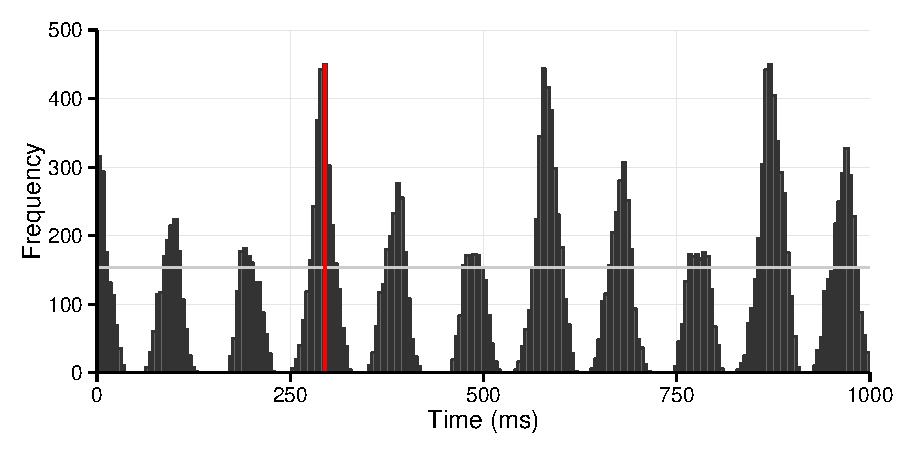
\includegraphics[width=0.8\textwidth]{figures/malawi/rttbin.pdf}
  \caption{$H(t)$ for flow displayed in Figure \ref{fig:hostlimited}. The horizontal line delimits $\overline{H}$ while the highlighted bin denotes the bidirectional RTT estimate.\label{fig:histogram}}
\end{figure}

%
% Explain why did we use FFT
%
The algorithmic recovery of $T$ from $H(t)$ presents additional challenges. 
In particular, $H(t)$ may include a large number of \ac{RTT} multiples, and a peak will be found for all of them. 
Crucially, all these peaks may be of comparable magnitude, complicating the task of selecting a single peak.
Moreover, these peaks need not be very pronounced, with histogram bins in close proximity of the peaks have very similar values as the peak itself. 
As such, taking \ac{RTT} candidates directly from $H(t)$ may result in a large set of similarly-valued bins situated around a peaks at multiples of the \ac{RTT}. 

Three recovery algorithms for $T$ are attempted.
First, as a baseline, the highest peak in $H(t)$ is selected as a candidate for $T$. 
In addition, expanding upon the work of Qian et. al. \cite{Qian:2009p429} a frequency-domain representation of $H(t)$ is used to identify $T$. 
This is done by selecting the highest peak of $|\hat{H}(\omega)|^2$, the \emph{energy spectral density} of $H(t)$ (i.e. the norm squared of the Fourier transform of $H(t)$). 
Finally, a custom utility-based technique that operates directly on $H(t)$ is proposed which achieves superior performance to both of the aforementioned methods.

%\subsubsection{FFT-Based RTT Recovery}
%We extract periodicity information from $H(t)$ by looking at $\hat{H}(\omega)$, the \emph{energy spectral density} of $H(t)$. Formally, $\hat{H}(\omega)$ is defined as the norm squared of the Fourier transform of $H(t)$, so that $\hat{H}(\omega) = |\mathcal{F}(H(t))|^2$. Using $\hat{H}(\omega)$ markedly improves the quality of our RTT estimation because the frequency peak corresponding to the RTT usually accounts for a much larger proportion of the total frequency domain energy than other peaks in $\hat{H}(\omega)$, leading to a much simpler discrimination of the true RTT. However, due to RTT changing during the lifetime of a flow, and also due to the expected noise associated with real-life data sources, $\hat{H}(\omega)$ can also occasionally include large peaks at frequencies unrelated to the RTT. In order to filter these out, we take a set of 10 frequency candidates from $\hat{H}(\omega)$, and use their associated periods as RTT candidates in our flow reconstruction algorithm (see Section \ref{
%subsection:malawi:flightAggregation}). We then select that RTT candidate which exhibits the smallest error, that is, that one which yields closest agreement with observed data.

%
% Algorithmic hacks
%
%To streamline our algorithm for streaming use, we use the following heuristics and approximations. Firstly, we define a range $[T_{\min}, T_{\max}]$ representing the range over which we find the RTT values of interest. Then, for each packet $p_j$, we build a subset $\mathcal{T}_j'$ of $\mathcal{T}_j$ by including all values of $t_j - t_k < T_{\max}$. We then generate $\mathcal{T}' = \cup_j \mathcal{T}_j'$ and approximate $H(t)$ by considering a histogram of the values in $\mathcal{T}'$. As usual, we do this by counting the frequency with which its values are observed in the ranges $[0,\tau)$, $[\tau, 2\tau)$, $[2\tau, 3\tau), \ldots$ where $\tau$ is the time resolution required. 


\subsubsection{Utility-Based RTT Recovery}
\label{sect:utilityBasedRecovery}

This method relies not on the identification of periodicities, but on explicitly matching experimentally found signatures. 
To this end, we consider the peaks of $H(t)$, which are then considered RTT candidates.  
However, trivial discriminators (such as simply selecting the highest peak) are not reliable. 
In this case, it was found experimentally that repeatable peaks and troughs also occur at multiples and sub-multiples of $T$, with the most important ones being $\frac{T}{3}$, $\frac{T}{2}$, $T$ and $2T$. 
We design this detection algorithm around the idea that a given pattern of peaks and troughs can identify $T$.

If we define $\overline{H}$ as the mean height of $H(t)$, we can define a per-peak utility function $p(t)$ so that 
\begin{equation*}
p(t) = 1.0 - \exp\left(-2.0 \left(\frac{H(t)}{\overline{H}}\right)\right) \mbox{.}
\end{equation*}
This function has several advantageous properties: it is 0 if $H(t)$ is zero, 1
if $H(t)$ is infinite, and $0.5$ if $H(t) = \overline{H}$.  In other
words it is a measure of the \emph{peakiness} of the data, with $p=1$ identifying
an infinitely high peak, $p=0$ identifying an empty histogram bin (trough), and $p=\frac{1}{2}$ 
implying that $H(t)$ is of exactly average height at that point. We can then score each candidate using the following utility function:
$$
P(t) = 1.5 p(t) + p(2t) - p\left(\frac{t}{2}\right) - p\left(\frac{t}{3}\right).
$$
That is, the candidate RTT $t$ scores highly if it is itself a peak, if it has a peak
at a multiple $2t$, and if it also manifests troughs at submultiples $\frac{T}{2}$ and $\frac{T}{3}$.
The factor of 1.5 was added after observations
showed that the peak at $T$ was the most important factor in determining
whether a candidate was the true RTT. Similarly, additional multiples and submultiples 
were excluded as they showed very limited discriminating power experimentally.

\begin{figure}
  \centering
  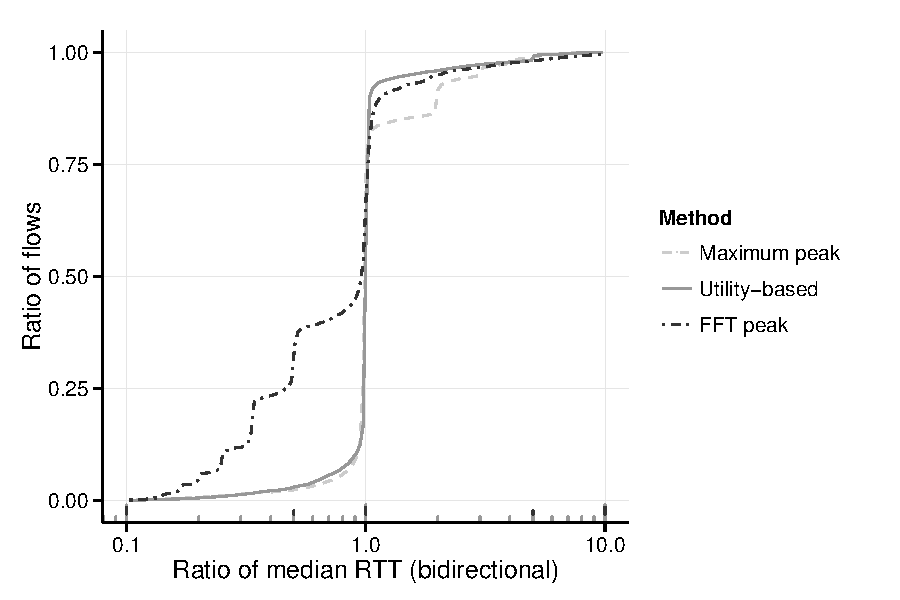
\includegraphics[width=0.8\textwidth]{figures/malawi/rttcomp.pdf}
  \caption{Accuracy of RTT estimator when compared to the median value of bidirectional estimate.}
\end{figure}

\subsubsection{Comparing RTT Recovery Algorithms}
\label{sect:comparingRecoveryAlgos}
As described in Section \ref{subsection:malawi:PeriodicEnhancement}, $H(t)$ is calculated in such a way that RTT periodicity is amplified. 
This means that FFT-based techniques could potentially perform better on $H(t)$ than on the packet stream with no pre-processing. 
However, this is complicated not only because $H(t)$ contains periodicities at multiples of $T$, but also discontinuities that generate harmonics at frequency multiples of the RTT fundamental. 
Hence, although the FFT $|\hat{H}(\omega)|$ of $H(t)$ is much cleaner than that of the packet interarrival time series on its own, its maximum peak rarely coincides exactly with the RTT clock (this corroborates reports by Qian et al \cite{Qian:2009p429}). 
Thus, applying the FFT leads to another \emph{peak detection problem} in which the RTT fundamental needs to be extricated from its harmonics and sub-harmonics. 
The trivial solution to this problem, the application of a bandpass filter around the RTT frequency, is of course unfeasible because the bandwidth and 
centring of such a filter depend on the RTT which is itself unknown.
The utility-based algorithm described in Section \ref{sect:utilityBasedRecovery} can hence be applied in either the time domain or the frequency domain; we chose to do it on the former on the interest of expediency and lower computational cost.

\newcommand{\RTTHeader}{Below & Above}
\newcommand{\SmallFlowName}{\textless 10MB}
\newcommand{\LargeFlowName}{\textgreater 10MB} 
\begin{table}
\footnotesize
\centering
\begin{tabular}{ p{1.5cm} p{1.2cm} p{0cm} p{.6cm}p{.6cm} p{0cm} p{.6cm}p{.6cm}}
& & & \multicolumn{2}{c}{Peak} & & \multicolumn{2}{c}{Utility-based} \\
\cline{4-5} \cline{7-8}
& Flow size & & \RTTHeader & & \RTTHeader \\
\cline{4-5} \cline{7-8} 
\multirow{2}{*}{Receiver side}  & \SmallFlowName && 4.31 & 9.13 && 4.58 & 6.35
\\ 
                                & \LargeFlowName && 6.72 & 6.43 & 4.97 & 5.33
\\
\multirow{2}{*}{Sender side}    & \SmallFlowName && 2.94 & 8.37 && 3.29 & 4.80
\\
                                & \LargeFlowName && 6.41 & 9.06 & 5.40 & 11.06
\\
\end{tabular}
\caption{\label{table:rttRecovery}Performance of RTT recovery algorithms}
\vspace{-3mm}
\end{table}

The performance of the analysed RTT recovery mechanisms is presented in Table \ref{table:rttRecovery}, that shows the percentage of total flows below and above the RTT range given by the bidirectional estimates.
We separate things for \emph{inbound} traffic (where we are positioned at the receiver side) and \emph{outbound} traffic (where we are positioned at the sender side). The utility-based algorithm is particularly useful to address RTT underestimation for flows over 10MB in size, which is our main objective since precisely that kind of estimation error would interfere with our ability to correctly decouple application behaviour from RTT-scale dynamics.


%For the most part, the utility based method improves on underestimation, which is our main objective since that would interfere with our flight reconstruction (i.e. generate lots of gaps).
%The exception (kind of) is traffic from the sender side, which in our training set (one week per year), had quite a lot of host limited traffic (paced out, no signal to recover).
%In this case, not a problem, since if the flow is long enough multiples of the RTT will still reveal host limitation, but will give us a smaller window..


\subsection{Flow Classification}
\label{subsection:malawi:flightAggregation}

One fundamental precondition to decouple the influence that network loss, host configuration and TCP behaviour has on the throughput experienced by a flow is the reconstruction of the congestion window behaviour of TCP flows on the basis of observed data. 
Unfortunately, the congestion window value is internal to the sender's TCP state machine and may not manifest itself in the absence of sufficient data from the application layer. 
A more easily observed quantity which serves as a reasonable proxy for the congestion window is the number of unacknowledged bytes in flight, henceforth referred to as the \textit{flight size}, which can be derived given an accurate estimate of the end-to-end delay.
The evolution of both flight size and RTT can in turn be used to ascertain to what extent throughput is regulated by limitations imposed at different layers of the networking stack.

% definitions
Given a candidate RTT, we can aggregate a stream of packets with arrival times $t_1, t_2, \ldots$ into a stream of \emph{flights}. 
Intuitively, a flight is a clustered subset of a TCP flow which exhibits its own temporal coherence; alternatively, it can be though of as a series of consecutive packets that were (roughly) generated by the sender as a response to the same protocol operation. 
A flight $f_i$ that begins
with the $j$th packet and ends with the $k$th is defined to have a \emph{total flight time} $\tau_i = t_{k+1} - t_j$. 
The algorithmic selection of initial and final packets in such a way that the resulting flights are indicative of TCP behaviour remains an open problem. 
Since we assume that the RTT provides a natural time frame for the operations of TCP, in the algorithm presented in this work, given an initial packet $\pi_j$ and an RTT estimate $T$, the $k$th (and final) packet is selected to minimise \emph{the flight time error} $e_i = |T - \tau_i|$. 
This mechanism follows closely the methodology described in \cite{Zhang:2002p85}, with the exception that we do not attempt to define flights as being both adjacent and disjoint; rather, we decompose flows into a stream of potentially overlapping flights. 
This helps the algorithm mitigate the deleterious effects of small deviations in the estimated RTT, which alters the properties of each flight. 
Furthermore, since the flight size is continuous in time, it makes little sense to restrict ourselves to a single sample per round trip time.

Having obtained flight information from each flow, we next consider what is the predominant factor that affects its throughput. 
Within the context of TCP, we classify flows as being artificially constrained by three distinct processes: \emph{application pacing}, \emph{host limited} and \emph{receiver shaping}.

\begin{figure}
\centering
  \centering
  \begin{subfigure}{1.0\linewidth}
    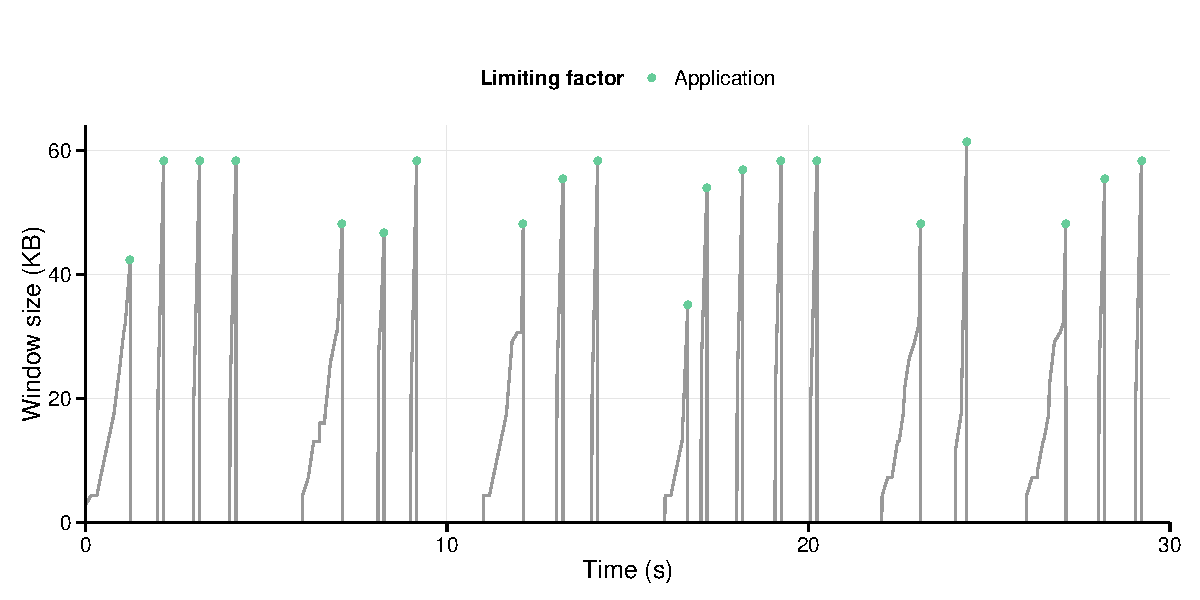
\includegraphics[width=1.0\textwidth]{figures/malawi/youtube.pdf}
    \caption{Application paced. \label{fig:youtube}}
  \end{subfigure}\\
  \begin{subfigure}{1.0\linewidth}
    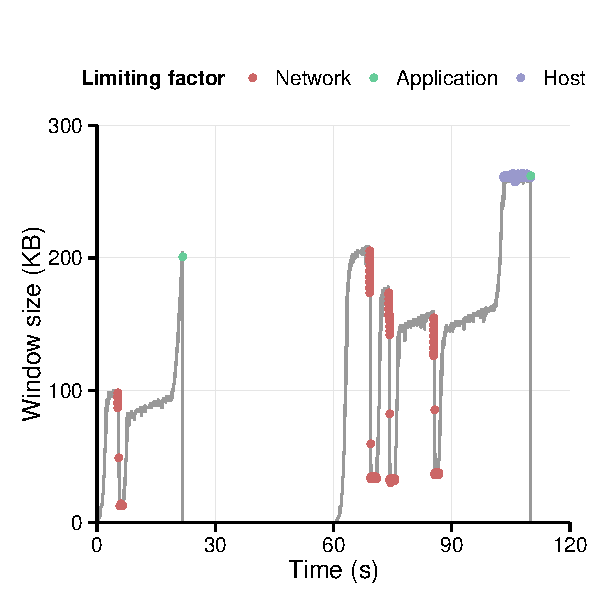
\includegraphics[width=1.0\textwidth]{figures/malawi/hostflow.pdf}
    \caption{Partially host limited. \label{fig:hostlimited}}
  \end{subfigure}\\
  \begin{subfigure}{1.0\linewidth}
    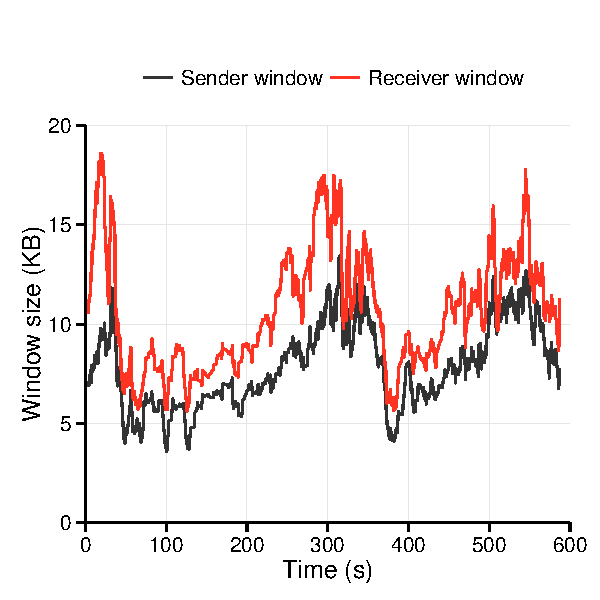
\includegraphics[width=1.0\textwidth]{figures/malawi/awnd.pdf}
    \caption{Receiver shaped. \label{fig:awnd}}
  \end{subfigure}
  \caption{Flight size over time for flows affected by different artificial constraints. \label{fig:kindsOfFlowEffect}}
\end{figure}


\subsubsection{Application Paced Flows}
\label{sssec:app}

A flow whose throughput decreases because it has no outstanding data to send is temporarily limited by the application. 
Flights can be identified as being \emph{application limited} if terminated with a packet smaller than the maximum segment size (MSS) and followed by an inter-arrival time greater than the RTT, as consistent with \cite{Zhang:2002p85}. 
The underlying reason for this defintion is that most TCP implementations will wait some time for subsequent bytes to be written to the socket if the next packet to be sent is smaller than the MSS, unless the TCP\_NODELAY option is set \cite{nagle1984rfc}.

A flow with \emph{application limited} flights however is not necessarily \emph{application paced}. In practice, all flows for which the final packet is observed contain at least one such flight.
For the purposes of our work, we are focused on identifying cases in which throughput is predominantly determined by application behaviour.
One such example is illustrated in figure \ref{fig:youtube}, in which a stream is delivered by periodically writing blocks to the sending socket.
The resulting network-level behaviour is distinct from traditional congestion control: short bursts are interspersed with protracted silence.
Application limited flights, which terminate on non-MSS packets, are highlighted at the end of each burst.

This behaviour is in stark contrast to that exhibited in figure \ref{fig:hostlimited}, where distinct transfers are multiplexed on top of a single transport association over time.
From the perspective of the network, there is little to distinguish the behaviour of such traffic from independent TCP flows.
Application paced connections such as Youtube traffic however exhibit a degree of regularity which can potentially be exploited by the network in predicting demand or smoothing bursts.

In order to identify such recurring behaviour, we identify flows as being \emph{application paced} if the period between bursts terminated by \emph{application limited flights} is consistently under 10 seconds and the standard deviation of the intermediate pauses is under one second.
This definition in particular purposely ignores flows which exhibit long silence periods due to user interaction, and follows closely the behaviour historically associated to Youtube streaming in particular.

\subsubsection{Host Limited Flows}
\label{sssec:host}

Given sufficient bandwidth and traffic to send, a flow may encounter local constraints at either end-host which cap its throughput. 
For instance, the buffer space allocated on both the sender and receiver side is often pre-configured, and it is common practice to tune these values down on popular servers and managed infrastructure in a bid to conserve memory or bandwidth.
A receiver is also limited in the window size it can announce to the remote sender; if the windowscale option \cite{jacobson1992tcp} is not negotiated during the TCP handshake, the advertised window cannot exceed 64KB.

In both cases, a local decision by either host can determine the upper bound of the flow rate.
These \emph{host limited} cases are characterised by a constant window size over time.
The methodology described for flight aggregation at the beginning of this section typically generates a large number of flights, representing many likely combinations given a base RTT estimate.
In order to identify the flat-lined behaviour of a host limited flow, we first filter the flight stream to remove some of the uncertainty derived from small fluctuations in the RTT.
We then select the maximum flight size observed for each RTT interval, and declare a sequence of flights to be host limited if the same maximum was observed over six consecutive RTTs (this is twice the period suggested in \cite{Zhang:2002p85}).
In practice, increasing the period over which the maximum window size is tracked allows us to more accurately discern between host limited behaviour and more conservative bandwidth probing, such as that performed during the convex phase of TCP CUBIC \cite{Ha:2008p471}.

A flow may be host limited for only brief periods of its lifetime, as illustrated in figure \ref{fig:hostlimited}.
To filter out such cases where host limitations are not the predominant factor in defining flow throughput, we further enforce that in addition to host-limited flights, the average window size must over a flow lifetime should be within 10\% of the inferred host limit, which is not the case in figure \ref{fig:hostlimited}.

In practice, flows can exhibit both application pacing and host limitations, with bursts being sent at a capped window size followed by application pauses.
In such cases, a flow will still be classified as being \emph{application paced} if it meets the requirements set out in the previous section, as doing so provides evidence that it controls throughput in spite of the degraded performance provided further down the stack. 
This line of reasoning applies equally to the occurrence of sporadic loss; so long as block delivery is ensured within the timeframe dictated by the application, it remains in control.

\subsubsection{Receiver Shaped Flows}
\label{sssec:rec}

A flow which is neither \emph{application paced} or \emph{host limited} can still be artificially constrained by flow control (rather than by congestion control).
Traditionally, in TCP the sender is responsible for regulating throughput. 
However, the receiver can also shape throughput by manipulating the \emph{advertised window} announced on every acknowledgement.
Such receiver-window auto-tuning has been available on Windows operating systems since Vista \cite{vistaReceiveWindow}, and can also be leveraged by middleboxes in order to throttle inbound traffic \cite{appEx}.

In order to evaluate the potential impact of such behaviour, we further propose a heuristic to identify receiver-shaped traffic.
For flows in which both directions of traffic are observed it is possible to correlate the evolution of the advertised window with the size of reconstructed flights.
Figure \ref{fig:awnd} displays an example of a receiver-shaped connection, in this case throttled by an intermediate middlebox.
Since the advertised window may be fluctuating, it is not always obvious which of the many updates were effectively applied by the sender as successive values supersede each other.
An example of a reconstructed flow which is subjected to receiver shaping is displayed in Figure \ref{fig:awnd}.

For flows in which both directions are observed, it is possible to classify flights as being receiver-shaped if there is a statistically significant correlation between the advertised window size and the maximum flight size observed.
Harnessing the stream filtering used in detecting host limited behaviour, we perform such analysis over a sliding window of 10 RTT intervals.
A flight is flagged as being receiver shaped if the correlation between receiver window and flight size is statistically significant; a flow is considered to be predominantly receiver shaped if over half of its flights are flagged as such.
We do not perform this covariance analysis on flights which contain out-of-order or retransmitted packets. 
In these cases, both the receiver and sender window sizes are correlated \emph{by definition}. 
In the former case, the receiver buffer will temporarily fill expecting the next packet in sequence, in the latter case, TCP will reduce its window.

Given that receiver shaping classification requires correlating information in both directions of a TCP connection, it will come as no surprise that the absence of the reverse path can introduce false positives into our measurements. 
This happens because any given flow might be receiver shaped in such a manner that the heuristic erroneously attributes its behaviour to host limitations. 
In the absence of additional evidence, this misclassification is difficult to detect explicitly. 
Instead, we calculate the ratio of receiver shaped flows which would have been incorrectly identified if the reverse path were not observed. 
This error rate can then be used to evaluate the accuracy of classifier results.

\section{Macroscopic traffic trends}
\label{section:malawi:macro}

\begin{figure}
  \centering
  \begin{subfigure}[b]{1.0\linewidth}
  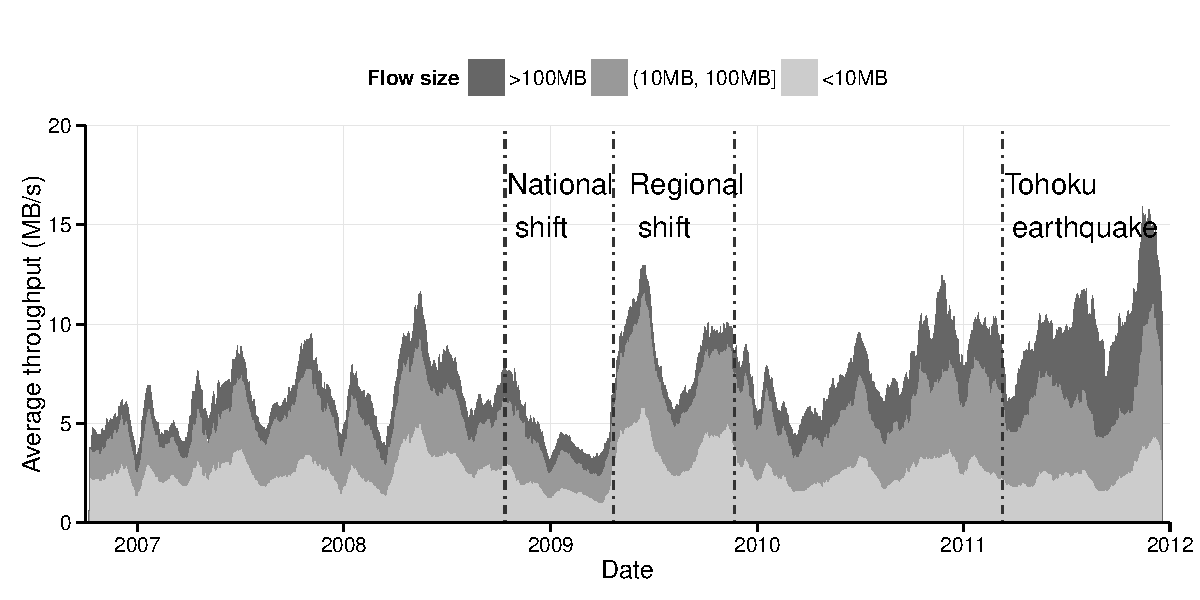
\includegraphics[width=0.9\textwidth]{figures/malawi/tput}
  \caption{Mean throughput}
  \end{subfigure}
  \begin{subfigure}[b]{1.0\linewidth}
  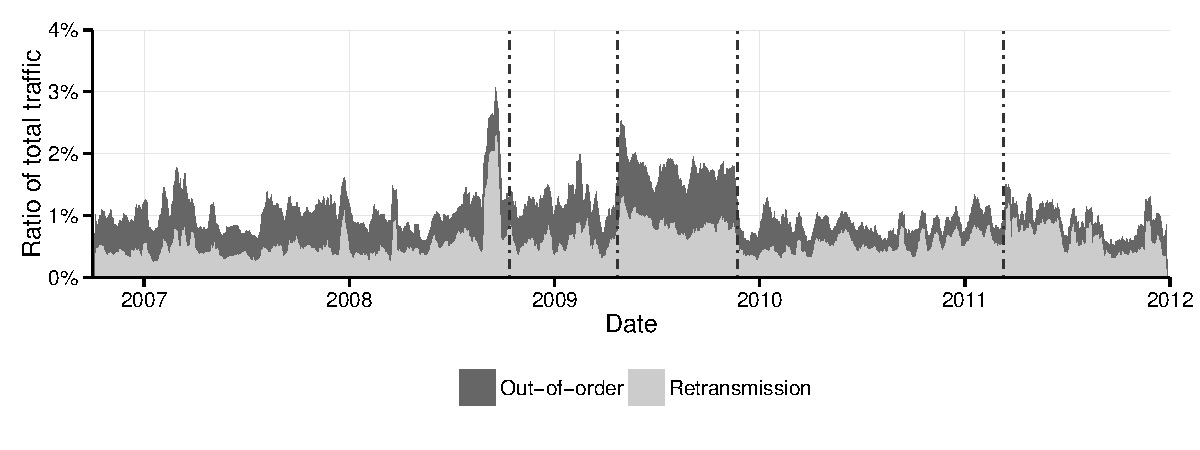
\includegraphics[width=0.9\textwidth]{figures/malawi/losses}
  \caption{Mean loss rate}
  \end{subfigure}
  \caption{Longitudinal evolution of inbound traffic.}\label{fig:MAWI}
\end{figure}

Over a five year period, changes in routing and application popularity have continually redefined the nature of traffic under observation.
This section provides a macroscopic view of these shifting trends. Figure \ref{fig:MAWI} displays the average throughput and loss ratio, calculated for TCP traffic only, smoothed on a weekly basis. 
Two routing changes internal to WIDE had significant impact on overall traffic, and are consequently highlighted.
The first, performed towards the end of 2008, diverted most of the inbound traffic from \emph{national} sources away from the monitored transit link, resulting in a reduction of traffic.
This event was preceded by increased congestion downstream from the monitoring point.
The second, in early 2009, saw a significant increase in \emph{regional} traffic from Asian neighbours, and was reverted approximately six months later. 
During this period aggregate end-to-end loss rates increased as a result.
While this is mostly due to the higher proportion of upstream congestion for traffic from Taiwan and China in particular, most traffic was adversely affected by the increased utilisation, suggesting that the transit link itself may have been a bottleneck during this period.
Finally, the impact of the Tohuku earthquake resulted in a noticeable break in demand coinciding with the start of the Japanese fiscal year in April, in which traffic traditionally ramps up.

\subsection{Geographic distribution}

\begin{table}\footnotesize
\centering
    \begin{tabular}{  
@{}
$>{\scshape}p{3.0cm}
^r
^r
^r
^r
^r@{\hskip 1.0cm}
^r
^r
^r
^r
^r
@{}
}
\toprule
\rowstyle{\scshape\bfseries}
\multirow{2}{*}{\parbox[][0.7cm][b]{3.0cm}{Country}} & 
\multicolumn{5}{c}{\scshape\bfseries{Outbound traffic (\%)\hspace*{0.45cm}}} & 
\multicolumn{5}{c}{\scshape\bfseries{Inbound traffic (\%)}} \\
\cmidrule(r{1.0cm}){2-6} \cmidrule{7-11}
\addlinespace[-0.6em] \rowstyle{\scriptsize\scshape}
 & 2007 & 2008 & 2009 & 2010 & 2011 & 2007 & 2008 & 2009 & 2010 & 2011 \\
\midrule

        United States & 27.3 & 31.3 & 29.3 & 36.4 & 35.7 & 45.7 & 41.5 & 53.3 & 65.1 & 67.1
\\
        \scriptsize{ California } & \scriptsize{ 39.0 } & \scriptsize{ 61.8 } & \scriptsize{ 63.5 } & \scriptsize{ 53.8 } & \scriptsize{ 50.6 } & \scriptsize{ 55.7 } & \scriptsize{ 47.9 } & \scriptsize{ 46.7 } & \scriptsize{ 24.9 } & \scriptsize{ 34.9 }\\\scriptsize{ Texas } & \scriptsize{  5.8 } & \scriptsize{  4.3 } & \scriptsize{  4.1 } & \scriptsize{  2.4 } & \scriptsize{ 13.9 } & \scriptsize{  7.0 } & \scriptsize{ 12.0 } & \scriptsize{  5.8 } & \scriptsize{  7.1 } & \scriptsize{  5.6 }\\\scriptsize{ Colorado } & \scriptsize{  1.9 } & \scriptsize{  1.2 } & \scriptsize{  0.6 } & \scriptsize{  8.5 } & \scriptsize{  2.8 } & \scriptsize{  4.9 } & \scriptsize{  6.0 } & \scriptsize{  5.9 } & \scriptsize{  9.7 } & \scriptsize{  5.8 }\\\scriptsize{ Virginia } & \scriptsize{  1.9 } & \scriptsize{  1.0 } & \scriptsize{  0.8 } & \scriptsize{  0.4 } & \scriptsize{  0.6 } & \scriptsize{  1.2 } & \scriptsize{  3.0 } & \scriptsize{ 14.1 } & \scriptsize{ 13.1 } & \scriptsize{  8.3 }\\\scriptsize{ Washington } & \scriptsize{  4.0 } & \scriptsize{  2.9 } & \scriptsize{  3.5 } & \scriptsize{  6.1 } & \scriptsize{  6.6 } & \scriptsize{  0.9 } & \scriptsize{  5.7 } & \scriptsize{  3.5 } & \scriptsize{  3.0 } & \scriptsize{  2.0 }\\\scriptsize{ New Jersey } & \scriptsize{  2.8 } & \scriptsize{  1.5 } & \scriptsize{  0.7 } & \scriptsize{  1.1 } & \scriptsize{  1.9 } & \scriptsize{  1.0 } & \scriptsize{  1.8 } & \scriptsize{  1.6 } & \scriptsize{  4.9 } & \scriptsize{ 13.6 }\\\scriptsize{ Massachusetts } & \scriptsize{  1.6 } & \scriptsize{  1.1 } & \scriptsize{  0.9 } & \scriptsize{  6.1 } & \scriptsize{  4.9 } & \scriptsize{  5.4 } & \scriptsize{  2.1 } & \scriptsize{  1.8 } & \scriptsize{  1.6 } & \scriptsize{  2.0 }\\\scriptsize{ Florida } & \scriptsize{  3.1 } & \scriptsize{  2.3 } & \scriptsize{  1.3 } & \scriptsize{  1.1 } & \scriptsize{  0.9 } & \scriptsize{  1.0 } & \scriptsize{  0.4 } & \scriptsize{  0.4 } & \scriptsize{  8.5 } & \scriptsize{  7.9 }
\\
        Japan & 11.6 & 15.4 & 17.7 & 16.7 & 16.1 & 33.8 & 32.2 &  7.3 & 8.1 & 11.5\\China &  7.9 & 20.5 & 17.8 & 10.3 &  5.9 &  2.5 &  5.3 &  6.3 & 4.6 &  3.1\\Korea, Republic of &  5.3 &  1.3 &  2.1 &  7.8 & 23.8 &  4.7 &  5.1 &  3.2 & 1.1 &  0.5\\Germany &  2.2 &  1.7 &  1.6 &  1.0 &  0.6 &  3.0 &  6.1 &  5.3 & 5.5 &  1.4\\Taiwan &  2.7 &  1.3 &  4.0 &  3.6 &  2.7 &  0.8 &  0.9 & 10.9 & 0.9 &  0.4\\Netherlands &  0.4 &  0.4 &  0.5 &  0.3 &  0.4 &  0.9 &  1.0 &  4.1 & 6.2 &  6.9\\India &  2.8 &  3.3 &  4.8 &  3.3 &  2.0 &  0.3 &  0.1 &  0.0 & 0.2 &  0.0\\France &  1.2 &  1.1 &  0.9 &  0.9 &  0.9 &  1.6 &  1.2 &  2.6 & 3.4 &  1.7\\United Kingdom &  1.1 &  1.0 &  1.0 &  0.9 &  0.7 &  2.5 &  2.2 &  1.6 & 1.3 &  1.3
\\
    \end{tabular}
  \caption{Percentage of inbound and outbound traffic by country\label{table:dest}. U.S. state values are relative to total national traffic.}
\end{table}



These changes are both visible in the geographic distribution of inbound traffic over time, shown in table \ref{table:dest}.
Prior to 2009, a significant proportion of transit traffic originated from within Japan. Over time, however, the ratio of traffic from Asia has been reduced. While this may foreshadow an increased concentration of traffic from the United States, it should primarily be viewed as a reflection of routing policy, with regional traffic being diverted to alternate routes as Japan became increasingly interconnected to its neighbours.


Further geographic shifts are apparent when breaking down US traffic by state.
The proportion of traffic originating from California has decreased over time, dropping from 55\% of total US traffic in 2007 to only 35\% in 2011.
In its place, a larger set of states have emerged as content providers, with New Jersey, Florida and Virginia contributing over a quarter of all traffic originating within the US by 2011.

%tip

Table \ref{table:dest} shows the geographic distribution of both inbound and outbound traffic since 2007. The majority of traffic flows to and from the United States, which has increased its share of bandwidth in either direction over the past five years. The proportion of traffic flowing from the United States is particularly high, accounting for almost 70\% of inbound traffic in 2011. While this may foreshadow an increased concentration of traffic within the United States, it should first be viewed as a reflection of routing policy, as regional traffic has been increasingly diverted to alternate routes. Inbound traffic from Japan, China, Korea and Taiwan have all been on the wane over the past five years as Japan has become increasingly interconnected to its neighbours. Of particular importance is the routing change at the end of 2008, which resulted in a sharp drop in inbound traffic from within Japan, with a net effect easily discernable in figure \ref{fig:inout}. This event had a profound influence in shaping not only the distribution of traffic, but also overall loss and delay as we shall observe in sections \ref{sec:delay} and \ref{sec:loss}.

A further point of interest is the breakdown of traffic from the U.S. by state. The overall increase in volume at a national level has broken the hegemony of California, which saw its overall share of inbound traffic fall from 60\% in 2007 to just under 40\% by 2011. In its place a larger set of states have emerged as content providers. Not listed are New Jersey, Florida and Virginia, which all saw sharp rises in 2011 to provide 35\% of all traffic from the U.S towards WIDE.
    
In the outbound direction, the geographic distrubtion of traffic is less skewed, with a greater proportion of traffic flowing towards Japan and China in particular. Due to a change in routing towards the end of 2010, traffic to Korea increases dramatically. In 2011, 12.7\% of all outbound traffic was destined to Korea Telecom alone. European destinations overall have a small proportion of outgoing traffic, which appears to be shrinking over time. The most significant factor for the discrepancy between inbound and outbound traffic for Europe as a whole is the timezone difference, as traffic is measured at 05:00GMT. This however does not account for why outbound traffic overall has been falling. Since most outbound traffic towards Europe at the time of measurement is likely to be scheduled transfers with no human intervention, a plausible explanation for this trend is the gradual shift away from file-sharing using peer-to-peer applications. This is further corroborated by the rise of hosting solutions which facilitate filesharing such as MediaFire, as shall become evident when analyzing the breakdown of traffic by AS.


\


\subsection{\acs{AS}-level distribution}
\begin{figure}
    \centering
    \begin{subfigure}[b]{0.5\linewidth}
        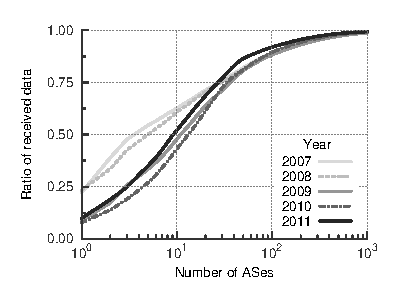
\includegraphics{figures/malawi/asn_cdf_in}
        \caption{Inbound}
    \end{subfigure}%
    \begin{subfigure}[b]{0.5\linewidth}
        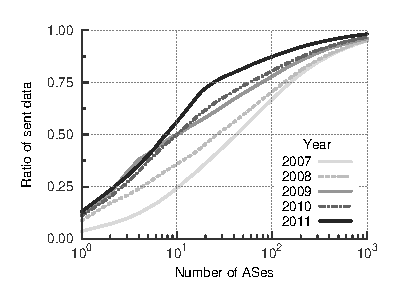
\includegraphics{figures/malawi/asn_cdf_out}
        \caption{Outbound}
    \end{subfigure}%
    \caption{CDF of inbound data by AS. \label{fig:ecdf_asn_from}}
\end{figure}


%\begin{table*}\scriptsize
%\centering
%\subfloat[2007]{
    %\begin{tabular}{
@{}
$>{\raggedleft}p{0.6cm}
^>{\scshape}p{2.25cm}
^>{\raggedleft\arraybackslash}p{0.6cm}
@{}
}
\toprule
\rowstyle{\scshape\bfseries}
\acs{ASN} & \acs{AS} name &
\% \\
\midrule

    %\input{data/malawi/asn2007.tex}
    %\end{tabular} % closes asnheader.tex tabular environment
    %}
%\subfloat[2009]{
    %\begin{tabular}{
@{}
$>{\raggedleft}p{0.6cm}
^>{\scshape}p{2.25cm}
^>{\raggedleft\arraybackslash}p{0.6cm}
@{}
}
\toprule
\rowstyle{\scshape\bfseries}
\acs{ASN} & \acs{AS} name &
\% \\
\midrule

    %\input{data/malawi/asn2009.tex}
    %\end{tabular} % closes asnheader.tex tabular environment
%}
%\subfloat[2011]{
    %\begin{tabular}{
@{}
$>{\raggedleft}p{0.6cm}
^>{\scshape}p{2.25cm}
^>{\raggedleft\arraybackslash}p{0.6cm}
@{}
}
\toprule
\rowstyle{\scshape\bfseries}
\acs{ASN} & \acs{AS} name &
\% \\
\midrule

    %\input{data/malawi/asn2011.tex}
    %\end{tabular} % closes asnheader.tex tabular environment
%}
%\caption{
    %\label{table:topASin}
    %Top 10 ASes for inbound traffic by year. Additionally listed is the ratio of aggregate end-to-end loss.}
%\vspace{-3mm}
%\end{table*}


These large-scale changes are a natural outcome of content consolidation. This is most apparent at the AS level, where a direct mapping to a commercial entity is forthcoming.
Figure \ref{fig:ecdf_asn_from} shows the cumulative distribution of inbound traffic by AS, while table \ref{table:topASin} lists the top ten AS by traffic volume for 2007, 2009 and 2011.
While in 2007 traffic was already consolidated across a small set of ASes, a significant portion of transit traffic was Asian: most traffic from NTT and Limelight originated from within Japan. Such traffic has gradually been pushed away from transit by 2011.
Large carriers such as Cogent, Level3, Hanaro, China Telecom have also seen their importance diluted by ASes known to harbour one-click hosting services such as Choopa, Webazilla, WZ Communications, Carpathia and LeaseWeb.
Many of the hosted websites facilitate the distribution of copyrighted content, and as such are not capable of growing large enough to expand beyond hosted infrastructure without risking prosecution.
% overall summary: content consolidation, delay, etc
Overall, the observed traffic patterns match the insights provided by Labovitz et al. on the changing nature of interdomain traffic in \cite{Labovitz:2010p175}.
The implications for transit traffic from an Asian perspective is less intuitive: with the increased adoption of content delivery networks and internet exchanges points, more transit traffic is being retrieved from further away as content in the US shifts east.


%tip
It has been widely noted that inter-domain traffic has significantly changed over the past decade, with an increasing proportion of traffic flowing to and from a dwindling set of both large content providers and consumer networks. 
This shift carries potentially significant ramifications for network operators. 
Content consolidation provides opportunities for network optimization as a wider set of traffic is contained within a smaller set of addresses. 
Improved transport heuristics or dynamic traffic engineering are both feasible solutions under such conditions if designing for the typical case, rather than the worst case \cite{Dukki}.

Traffic consolidation is most apparent at the AS level, where a direct mapping exists to a commercial entity. 
How this translates down to the network layer is less clear. 
We start by investigating how traffic is distributed by both AS and network prefixes for inbound traffic, as shown in figure \ref{fig:ecdf_from}. 
Over the past five years, traffic has remained consistently concentrated in the top 100 ASes, accounting for approximately 90\% of all data received. 
Between 2008 and 2009, traffic to NTT (AS2914) dropped significantly as a wide range of Japanese prefixes were rerouted through a different ingress. 
Additionally, traffic from Limelight ceased to be visible from our measurement point. 
Together, they contributed over 30\% of all inbound traffic in 2007 and 2008. 
This explains the discrepancy in distribution between 2008 and 2009.

For outbound traffic, shown in figure \ref{fig:ecdf_to}a, consolidation has been much more perceptible. 
For the top 10 ASes alone, the proportion of traffic has more than doubled between 2007 and 2011. 
By 2011, the distribution of traffic amongst ASes for inbound and outbound traffic bears a striking similarity. 
The nature of this concentration is markedly different however, as made apparent by the distribution of traffic over network prefixes. 
The one hundred most popular network prefixes contribute 75\% of inbound traffic, yet only account for 50\% of outbound traffic. 
This matches our expectations on the inherent differences between large ISPs, which reflect the heterogeneity of their customer base through addressing, and content providers and CDNs concentrating resources in fewer locations. 



To further highlight this trend we display the top 10 ASes for both inbound and outbound traffic for 2007 and 2011 in tables \ref{table:topASout} and \ref{table:topASin} respectively. For each table we list the number of observed networks - networks belonging to that AS to which traffic was routed to over the entire year - the number of network prefixes which belong to the top 10000 networks and the ratio of traffic. Additionally, we display the values of the latter two values for prefixes with mask values greater than 19.

    For inbound traffic, both large consumer networks and content providers coexist in 2007. Youtube, Limelight, Google, Akamai and AcroNOC all send traffic almost exclusively from smaller address blocks. Additionally, most observed networks are amongst the highest ranked prefixes for inbound traffic, as opposed to large providers like NTT and Cogent, who have a much larger set of address blocks, but many of which do not have significant traffic. By 2011, NTT is the only ranked AS which still exhibits such behaviour for inbound traffic.

    Outbound traffic differs in many respects. Firstly, traffic was much less concentrated in 2007, with top ranked Google receiving a mere 3.6\% of all traffic. The remainder of the list is mostly compromised of large providers receiving most traffic through less specific prefixes. Curiously, NTT displays different patterns between inbound and outbound traffic, with a tendency to send from less specific prefixes, and receive to more specific ones. 

    In 2011 Korean telecom company KIXS exhibits a similar behaviour.  %WHY ??

    In this section we have shown how traffic consolidation has occured at different paces depending on the direction of traffic. Inbound traffic already showed strong signs of concentration in 2007, whereas outbound traffic has become dominated by large consumer networks and regional providers over the past five years. For both cases, traffic has converged towards similar distributions when analyzed by autonomous system, but the impact on routing seems markedly different. We will next focus on how these trends affect end-to-end traffic.


\subsection{Delay}
 
While understanding where traffic flows to and from is of great value at an operational, commercial and often political level, it portrays a small part of a wider picture. 
For end-users it is of less concern where content is being retrieved from or routed through compared to how long it takes.

\begin{figure}
    \centering
    \begin{subfigure}[b]{0.5\linewidth}
        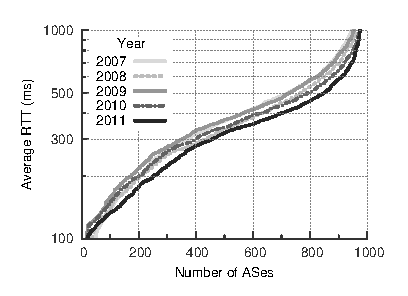
\includegraphics{figures/malawi/rtt_cdf_in}
        \caption{Inbound}
    \end{subfigure}%
    \begin{subfigure}[b]{0.5\linewidth}
        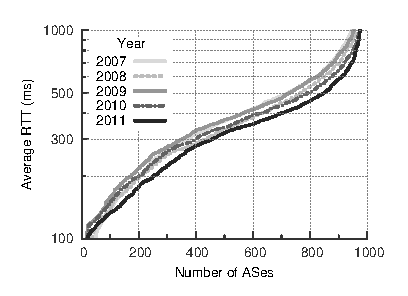
\includegraphics{figures/malawi/rtt_cdf_out}
        \caption{Outbound}
    \end{subfigure}%
    \caption{CDF of RTT by AS. \label{fig:rtt_cdf}}
\end{figure}

\begin{figure}
    \centering
    \begin{subfigure}[b]{0.5\linewidth}
        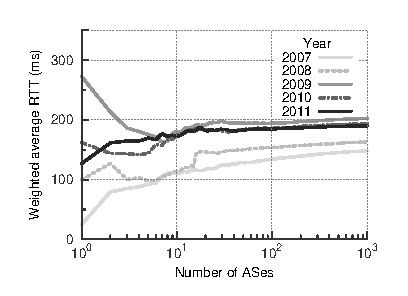
\includegraphics{figures/malawi/rtt_wcdf_in}
        \caption{Inbound}
    \end{subfigure}%
    \begin{subfigure}[b]{0.5\linewidth}
        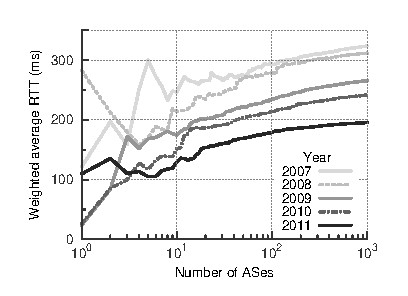
\includegraphics{figures/malawi/rtt_wcdf_out}
        \caption{Outbound}
    \end{subfigure}%
    \caption{CDF of weighted RTT by AS. \label{fig:rtt_wcdf}}
\end{figure}

The respective cumulative distribution functions of delay is display in figure \ref{fig:rtt_ecdf}. As with traffic distributions, the plots once again illustrate the same overall trend in subtly different patterns. Overall, delay has been decreasing over time, with the notable exception of a small segment of inbound traffic for network prefixes, mostly based in Japan, which were rerouted at the end of 2008. The rate at which delay has improved however seems markedly different. 

Comparing plots at the AS granularity, for the top 400 ASes delay has dropped by 20ms between 2009 and 2011 for inbound traffic, while the equivalent decrease for outbound traffic has been closer to 50ms. The absolute values in both cases are still disparate: over 90\% of ASes are reached within a round trip time of approximately 400ms when ranked by inbound traffic, whereas the equivalent value for outbound traffic is almost 200ms higher. This same trend is apparent when looking at delay by network prefix.

For inbound traffic the average RTT is low enough that geographical properties are clearly visible. A first plateau close to 100ms is apparent for traffic to the american west coast, while traffic to european destinations is clustured close to 250ms. Tellingly, this second plateau seems to be receeding in both AS and network plots. When taken in conjunction with the geographic distribution of traffic presented in table \ref{table:dest} this seems to confirm our suspicions that there has indeed been a reduction in the number of sources within Europe. 

A pertinent question at this point is in trying to understand how delay relates to traffic volumes. Given the different nature of stakeholders monopolizing traffic at either end of the spectrum, what can we say about the evolution of delay in either case? To assess this we plot the cumulative distribution of the average RTT weighted by the respective volume of traffic, as shown in \ref{fig:wrtt_ecdf}. In interpreting such plots one should keep in mind that they provide a rough indicator of the average delay to be expected if one were to sample a packet belonging to the top $N$ sources or destinations. As $N$ increases, we will approach the average RTT for all traffic in a given direction.

Inbound traffic by AS highlights and expected rise in delay between 2008 and 2009, as both NTT and Limelight are replaced by more distant sources. However, from 2009 onwards the overall delay is remarkably similar. While the cumulative distribution function of RTT shows improvement in delay at the tail, this results in very little improvement overall as traffic is dominated by a handful of entities.

Focusing on inbound traffic by network prefix not only confirms this, but actually shows that average delay has increased consistently over time.
In this case, the cumulative distribution of delay from \ref{fig:rtt_ecdf}b improved between 2009 and 2011, yet the average weighted RTT increased almost twofold for the top 10 network prefixes over the same period.

Two explanations emerge for this behaviour. The first stems from the changing nature of the traffic we are sampling. While functionally NTT represents the same entity over time, the traffic we observe is very different. As local traffic has increasingly been exchanged over peering links our view of traffic has stretched further afield. To illustrate this, one needs only notice that the average delay towards NTT, the top AS for inbound traffic in both 2007 and 2011, increased by approximately 100ms in figure \ref{fig:wrtt_ecdf}a. This does not represent a degradation in quality of service, but rather a change in where traffic is flowing from within the AS.

A further reason relates to the placement of content. As we had previously shown in \ref{table:dest}, there appears to be a migration of content away from California. Hosting sites such as Lemuria (Hotfile), based in Florida, Mediafire, based in Texas and District of Columbia and Carpathia, based in Virginia, are all contained within the top 20 ASes and have shifted traffic further from locations which had traditionally benefitted from low latency as viewed from Japan.

Analyzing the outbound traffic we seemingly get the opposite effect, with the average weighted RTT for the top 1000 ASes dropping by over 100ms. Once more, there is no single reason which accounts for the entirety of this effect. In 2007 many of the top destination ASes were in developing Asian countries, where infrastructure has improved greatly since. Improvements in routing to countries such as China and Korea have also had a positive net effect. This is visible in figure \ref{fig:rttyearcomp}, where the average RTT aggregated by country is plotted. For clarity, we filter out countries for which RTT estimates are available for less than 50 days in a year. Between 2007 and 2009 most Asian and European countries experience significant improvements in RTT. Those which don't tend to experience lower delays. Between 2009 and 2011 most countries reduce delay below 500ms. 

Finally, many of the very same companies which have had an effect of increasing RTT for inbound traffic, such as Mediafire or Ustream.tv, are also amongst the top destinations of traffic. It is interesting to note that as of 2011, data travelling from the top 1000 AS traffic sources is expected to experience the same latency as data travelling towards the 1000 most popular AS traffic destinations. In 2007, the value was two times higher for outgoing traffic.


\begin{figure}
    \centering
    \begin{subfigure}[b]{0.5\linewidth}
        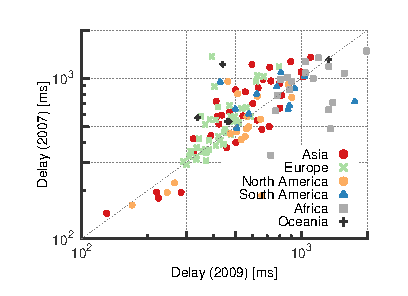
\includegraphics{figures/malawi/rtt_comp_07_09}
        \caption{Inbound}
    \end{subfigure}%
    \begin{subfigure}[b]{0.5\linewidth}
        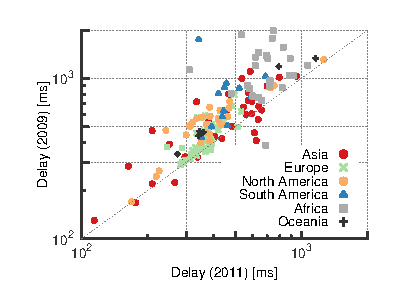
\includegraphics{figures/malawi/rtt_comp_09_11}
        \caption{Outbound}
    \end{subfigure}%
    \caption{CDF of weighted RTT by AS. \label{fig:rtt_comp}}
\end{figure}


\section{Performance Analysis}
%4.1) Balancing between two paths with high loss using fixed time unit
% using only loss-based balance in a simple regime where that works.
% Show how this converges quickly when one path suddenly gains
% background traffic (and hence loss).
%4.2) Balance between several paths with high loss and fixed time unit
% in simple regime where that works.
%4.3) Introduce experiment where equi-path is needed for probing and
% conservative is needed for low loss regime.
%4.4) Introduce experiment where time-scale tuning is needed to get
% good assessment of loss in low traffic regime.

This section evaluates \ac{PREFLEX} through simulation using ns-3 \cite{ns3}. 
Evaluating traditional traffic engineering methods typically involves abstracting traffic as flow aggregates, making large scale network performance analysis tractable.
\ac{PREFLEX} however balances traffic using loss rather than load, and focuses on improving end-user metrics as opposed to minimizing maximum link load.
As such, evaluating the proposed congestion balancer requires simulating end-to-end behaviour of traffic.

\subsection{Methodology}
\label{section:methodology}

Experimental validation is performed using the network topology displayed in figure \ref{fig:topo}. 
The topology links a client domain $C$ to a server domain $S$ through $N$ paths with equal bottlenecks $L_i$, and total bandwidth $B=\sum{L_i}$. 
While a domain is represented as a single entity in figure \ref{fig:topo}, each domain is composed by a traffic generator connected to a router. 
Client $C$ generates $G$ simultaneous \ac{HTTP}-like requests (or ``gets") from $S$ according to a specified distribution, described at the end of this section. 
As traffic flows from $S$ to $C$, the router within $S$ is responsible for balancing traffic over all available paths.

\begin{figure}
    \centering
    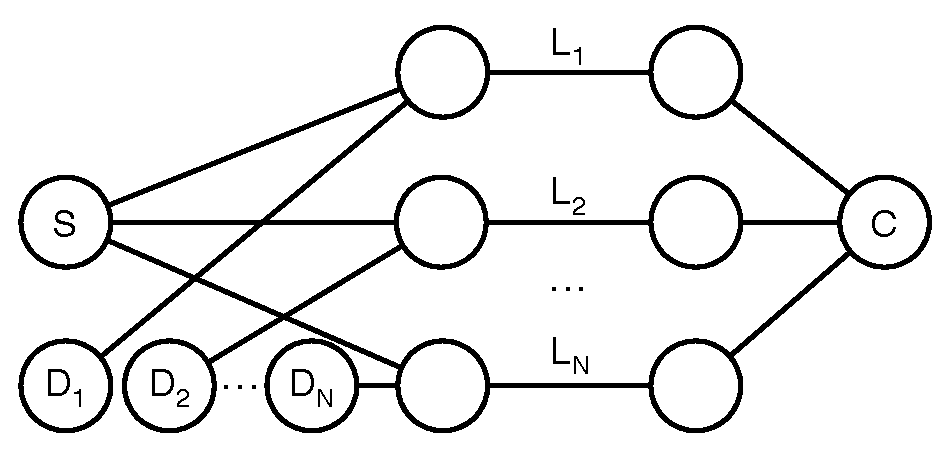
\includegraphics[width=2.5in]{figures/cate/topo}
    \caption{Simulation topology}
    \label{fig:topo}
\end{figure}

Across simulations, as the number of paths increases, total bandwidth $B$ and the number of simultaneous requests $G$ is fixed, providing insight into how efficiently \ac{PREFLEX} balances traffic as the granularity with which it can split traffic becomes coarser.

In order to evaluate how \ac{PREFLEX} shifts traffic in response to loss, additional ``dummy" servers $D_i$ are connected to $C$ through bottleneck link $L_i$.
The simulation runs for time $T$ and is partitioned into $N+2$ intervals starting on $s_i$, in which $s_0$ and $s_{N+1}$ have no traffic to $D_i$. 
Starting at time $s_i$, client $C$ generates $g_i$ requests to $D_i$ according to the same distribution as used to server $S$. 
All requests to $D_i$ end at time $s_{N+1}$. 
Equation \eqref{eq:si} sets the start time $s_i$ for requests to $D_i$ as a function of total simulation time $T$ and number of paths $N$. 
Likewise, equation \eqref{eq:gi} sets the number of simultaneous requests $g_i$ to $D_i$ as a function of $G$, the total number of requests to $S$, and $N$.
\begin{equation}
s_i = T\frac{i}{N+2}
\label{eq:si}
\end{equation}
\begin{equation}
\theta_i = \frac{\frac{1}{N+1-i}}{\sum{\frac{1}{N+1-i}}},  g_i = G\theta_i.
\label{eq:gi}
\end{equation}

Figure \ref{fig:demand} illustrates the number of simultaneous gets from $C$ to $D_i$ for $N=2$ (used in the example shown in figure \ref{fig:two}) and $N=4$. 
Generating cross-traffic in this manner serves two purposes. 
Firstly, $\sum{g_i}=G$, so independently of the number of concurrent paths, the maximum load in the system is $2G$. 
However, as the number of paths increases, the fluctuation in load for each path becomes smaller, stressing the sensitivity with which \ac{PREFLEX} must balance traffic. 
Secondly, the number of requests for each $D_i$ over time is the same. 
Over timescale $T$, equalisation appears to be an acceptable strategy but will however be shown to fail to make efficient use of available capacity. 
This is a fundamental limitation of offline traffic engineering, which is calculated over very long timescales and is unable to adapt as traffic routinely shifts.

\begin{figure}
    \begin{subfigure}[b]{.5\linewidth}
        \centering
        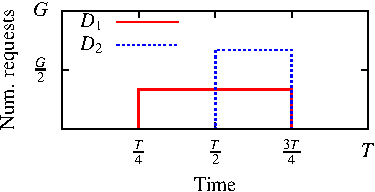
\includegraphics[width=2.25in]{figures/cate/dummy2-crop.pdf}
        \caption{$N=2$}\label{fig:1a}
    \end{subfigure}%
    \begin{subfigure}[b]{.5\linewidth}
        \centering
        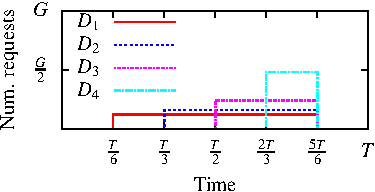
\includegraphics[width=2.25in]{figures/cate/dummy4-crop.pdf}
        \caption{$N=4$}\label{fig:1b}
    \end{subfigure}
    \caption[Number of requests to cross traffic servers.]{Number of requests from $C$ to cross traffic servers $D_i$ for different values of $N$}
    \label{fig:demand}
\end{figure}

The settings used for all simulations, including those previously shown in figure \ref{fig:two}, are as follows.
Total simulation time $T$ is set to $1200$ seconds, while total bandwidth $B$ is fixed at $240$Mbps. 
The number of requests $G$ sent from $C$ to $S$ is set to 240. 
Upon completing, a request is respawned after an idle period following an exponential distribution with a $15$s mean. 
Transfer size follows a Weibull distribution with an average value of $2$MB. 
While artificial, these values attempt to represent traffic to a single prefix with a file size that mimics the small but bursty nature of web traffic, which does not lend itself to being balanced by the end-host. 
\ac{PREFLEX} is configured with $\beta_E = 0.05$, $\mu_{min}=0.01/N$ and $\delta=0.005$.

\subsection{Varying bottleneck distribution}

For the remainder of this section, congestion balancing using \ac{PREFLEX} will be directly compared to equalisation, which mimics existing traffic engineering techniques based on hashing flow tuples for path assignment.
A useful reference point in interpreting results is to examine the case where all bottlenecks share the same bandwidth, $L_i=B/N$.
Under such conditions, figure \ref{fig:goodputeq} shows the goodput, calculated as the total data transfered to client $C$ by flows completed within $T$, as a proportion of total link bandwidth.
The bulk of goodput originates from server $S$, which is the only multi-homed domain.
If traffic is correctly balanced, servers $D_{1-N}$ should generate the same amount of goodput.
While both equalisation and congestion balancing saturate most available bandwidth, the former leads to disproportionate distribution of goodput amongst competing traffic. 
As loss is not equalised over all paths, the amount of goodput achieved by servers $D_i$ differs despite demand being similar.
\begin{figure}
    \centering
    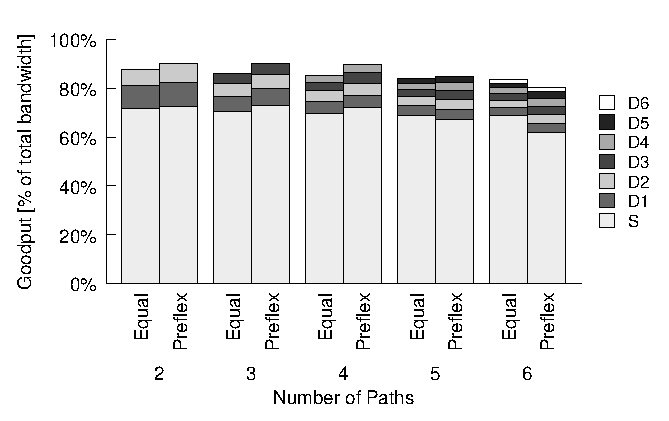
\includegraphics[width=4in]{figures/cate/eqbw}
    \caption[Goodput achieved over equal capacity links.]{Goodput relative to $B$ achieved by each server over equal capacity links.}
    \label{fig:goodputeq}
\end{figure}

In this scenario, equalisation can be seen as the optimal static TE solution, yet both approaches bear similar performance. 
With no knowledge of topology, link bandwidth or expected traffic matrices, \ac{PREFLEX} is able to adequately mimic the performance of the static TE solution for the case where such an approach is best suited.

\begin{figure}
    \centering
    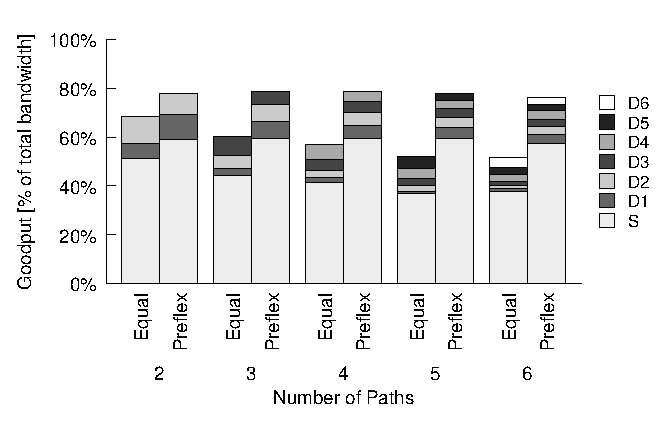
\includegraphics[width=4in]{figures/cate/diffbw}
    \caption[Goodput achieved over unequal capacity links.]{Goodput relative to $B$ achieved by each server over unequal capacity links.}
    \label{fig:goodputdiff}
\end{figure}

Where bottleneck bandwidth is unequal however equalisation is shown to be severely lacking.
The effect of differing bottlenecks is investigated by repeating previous simulations with the same total bandwidth $B$, but with $L_i$ set proportionally to $B$ in a similar manner to \eqref{eq:gi}, that is $L_i = \theta_i B$.
The ensuing results, shown in figure \ref{fig:goodputdiff}, highlight two significant shortcomings of equalisation which \ac{PREFLEX} overcomes. 
Firstly, goodput for $S$ drops as $N$ increases. 
Unable to realize it is overloading a path, equalisation is reduced to sending traffic over each link at approximately the same rate as the most congested link. 
In contrast, \ac{PREFLEX} detects congestion and adapts accordingly. 
Secondly, the incorrect distribution of traffic due to equalisation in $S$ distorts the goodput of competing traffic. 
While in \ac{PREFLEX} goodput from $D_{1-N}$ is perfectly balanced, with equalisation traffic crossing the most congested links are directly affected by another domain's inability to distribute traffic appropriately.
It may seem unfair to judge equalisation for cases where there is a mismatch in link capacity.
However, such a mismatch between link weight and path capacity arises regularly as operators adjust traffic engineering according to local conditions, with little thought spared for the impact this may have further downstream.

\begin{figure}
    \centering
    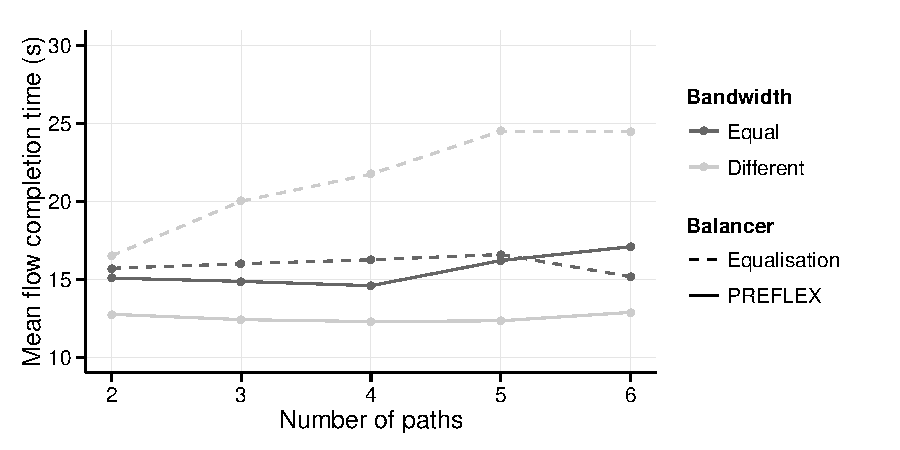
\includegraphics[width=3.2in]{figures/cate/duration}
    \caption[Mean flow completion time.]{Mean flow completion time for equal and differing bottleneck links.}
    \label{fig:duration}
\end{figure}

This impact is in turn perceived by users, who experience longer flow completion times, as shown in figure \ref{fig:duration}. 
In the equal bandwidth case the flow completion time is similar for both balancers.  
Where bandwidth differs however, balancing by congestion outperforms equalisation and maintains a stable performance even for all six paths.  
This shows that the algorithm scales well as the number of available paths increases. 

\section{Closing the loop}

This chapter broadly describes an architecture which shares the responsibility for resource pooling between end-hosts and edge networks, but does not explicitly dictate an outcome. \ac{PREFLEX} has been designed to take into account the inevitable tussle which will occur between both, and envisages use cases where control over resource pooling could feasibly shift entirely in one direction or the other. 

At its most liberal, \ac{PREFLEX} enables resource pooling to be entirely performed by end-hosts. At its most conservative, \ac{PREFLEX} affords edge network providers more fine-grained control over traffic than before. Between either extreme, the resulting mutualistic architecture offers greater transparency, control and robustness by realigning the interface between network and transport in order to accommodate the needs of both.

In order to make \ac{PREFLEX} deployable, the scope of the architecture has been restricted to stub domains.
While this necessarily reduces the amount of path diversity which can be explored, there are compelling reasons to abdicate some flexibility in favour of a more practical solution:

\begin{itemize}
\item{
    \textbf{Most benefit derives from a limited set of paths}.
    Work on source routing \cite{Gummadi:2004p131,Yang:2006p405} suggests most improvement in resilience can be extracted from a small set of deflections.
    Stub domains such as \acp{ISP} and enterprise networks are naturally multi-homed, and can provide reasonable path diversity given an adequate selection of providers.
    Expecting the establishment of cross-domain paths has been a pitfall for previous research in \ac{QoS} in particular and is marred by difficulties in providing incentives for all parties involved.
}
\item{
    \textbf{Stub domains are most aligned with user interests}. 
    For enterprise, academic and content distribution networks, end-hosts are typically managed by the same entity which operates the network.
    For \acp{ISP}, there is a binding contract between end-users and provider.
    In either case, the stub domain not only benefits from not deteriorating the quality of service provided to hosts locally, but also has an interest in making sure end-to-end traffic is unaffected by outages or degraded performance.
    The inability to reach a website is often misdiagnosed by users as a failure of the stub domain, rather than the intervening network path or the remote host.
    As a result, the burden of remote failures is often placed on local customer support.
    \ac{PREFLEX} allows resources not only to be shared more efficiently, but also potentially reduces the impact of remote network events on stub domains.
}

\item{
    \textbf{The Internet topology is flattening}. 
    In studying over 100 \acp{ISP}, transit providers and content providers for over two years, Labovitz \emph{et al.} \cite{Labovitz:2010p175} established the changing nature of the Internet topology, migrating from a hierarchy of providers to an increasingly interconnected model.
    The rise of \acp{IXP} where customer networks peer directly with content providers has had a profound impact in shaping traffic patterns and interdomain traffic in particular.
    The length of \ac{AS} paths has decreased for most \emph{content}.
    As a consequence, it has become simpler for a stub domain to ensure path disjointness as a larger portion of the end-to-end path is under its control.
}
\end{itemize}

The resulting architecture provides many benefits. 
Balancing is both transport agnostic and allows flow state to be kept to a minimum, requiring policing at the edges only if congestion accountability is required. 
Additionally, path selection is receiver driven, aligning the stakeholder who can decide when to issue \ac{FNE} packets with the stakeholder who benefits the most. 
The key to path selection is the information provided by the sender (point 7 in figure \ref{fig:preflexout} ), which allows the network to estimate path loss on the same timescale as hosts. 
By pooling loss information from multiple hosts, the network may additionally be made aware of path failures sooner than hosts using \ac{TCP} inference.

%We assume for the entirety of this section that each flow follows a single path and that a host does not override the path selected by its network, although neither is strictly necessary. 
%The implications of both assumptions being broken and the incentives involved are briefly reviewed in \cite{Araujo:2010p224}.


\chapter{A longitudinal analysis of \acs{TCP} traffic}
\label{chapter:malawi}

\renewcommand{\locfolder}{\chapfolder/malawi}
While the Internet has become evermore interconnected, exploring path diversity has been relegated to an afterthought in an architecture modeled around assumptions that no longer stand. 
Single-path forwarding as a paradigm arose not as a guiding principle, but as a natural aversion towards increasing both the complexity and cost of a resource starved network.
%engineering for scarcity worked, but cracking
Engineering for scarcity has propelled the Internet to an unprecedented scale, but problems arise when what was otherwise scarce becomes plentiful. 
Protocols designed to be bit conservative at the expense of latency have become technological anachronisms as bandwidth costs continue to plummet. 
Similarly, the notion of a router as a device merely capable of forwarding packets has long been obsolete as Moore's law continues to pave the way for greater functionality within the network. 
\ac{NAT}, \ac{DPI} or \ac{PEP} are all examples that when it comes to drawing a boundary between network and transport, the line begins to blur \cite{Ford:2008p34}.

%% paralelism increasing
Furthermore, parallelism seems to be a dominant trend at every level of the Internet architecture as a cost-effective means of increasing both performance and robustness. 
At the inter-domain level, the \ac{AS} graph is becoming flatter and more highly interconnected \cite{Haddadi:2010p129}. 
Within domains, the sheer complexity of managing paths has led to the streamlined design and deployment of \ac{MPLS} \cite{Rosen:2001p147}, implementing a fully fledged layer in its own right. 
At the edges the rise in multi-homing continues to increase the strain on an already overloaded routing architecture. 
Even within network components, parallelism is such that packet re-ordering can no longer be considered pathological \cite{Bennett:1999p120}.

Given these trends, one would expect the ability to pool traffic across such emergent path diversity to have become a network primitive. 
In reality, each stakeholder in the Internet architecture seems to balance traffic according to their needs while attempting to remain inconspicuous to others. 
At best, this interaction between stakeholders can be seen as a form of commensalism, where one entity can extract benefits while others remain unaffected. 
At worse, the competitive nature of the tussle \cite{Clark:2005p67} that ensues can spiral into a situation where few profit.

This chapter investigates the nature of this antagonism between network and endpoints and reflects on how the Internet can accommodate the needs of both through the use of \ac{PREFLEX}, a proposed architecture for balancing congestion which foments mutualism between end-hosts and edge network providers.

\section{Related work}
\label{section:malawi:related}

Despite their inherent value, longitudinal studies of Internet phenomena are rare. 
Over its short lifespan the Internet has been shaped as much by technological change as by political and commercial realities. 
This dynamic nature does not lend itself to observational studies where data must be collected and curated over long periods of time, and has resulted in a scarcity of relevant datasets. 
What few exceptions exist often stem from collaborative research efforts, such as CAIDA \cite{CAIDA} or Oregon Routeviews \cite{routeviews}. 
The usefulness of these datasets however can be severely affected by the need for data privacy. 
The dissemination of interdomain routing information, where no such requirement exists, has assisted in a wealth of research on wide ranging topics, from quantifying path diversity \cite{Oliveira:2009p203} to locating Internet bottlenecks \cite{Hu:2004p96}. 
In contrast, longitudinal datasets relating to passive measurements have nurtured a much smaller community of researchers often focusing on characterizing traffic \cite{Fontugne:2010p413}. 
Stripped of the locality contained within IP addresses however, researchers are left unable to relate these findings to a wider context.
Instead, cross-sectional studies characterizing traffic aggregated by location are frequently conducted under different contexts \cite{Ager:2011:WCC:2068816.2068870}, but lack the temporal perspective only longitudinal studies can afford. 
Efforts to characterize the spatial properties of traffic over time \cite{Dhamdhere:2011p428,Labovitz:2010:IIT:2043164.1851194,Cho:2008:OSC:1544012.1544024} have defined the changing of Internet topology and traffic alike but fall short of relating such shifts with their impact on relevant metrics such as loss or delay. 

% other work since
This chapter builds on a wealth of prior work on understanding Internet traffic and serves as a reappraisal of significant past contributions.
Flow characteristics and \ac{TCP} behaviour at large are subject to frequent reassessment \cite{Zhang:2002p85}.
Of particular relevance to the current work are passive studies which delve into the inner mechanisms of \ac{TCP}.
In \cite{Jaiswal:2004p242}, Jaiswal et al.\ infer the sender's congestion window by identifying the congestion control variant from the behaviour observed during loss recovery.
The use of separate state machines for each variant however proves unscalable given the many flavours of \ac{TCP} congestion control which have since been deployed.
In \cite{Lan:2006p566}, Lan et al.\ analyse flows according to size, duration, rate and burstiness and characterise the observed correlations for heavy-hitters specifically,
uncovering evidence of increased application influence on flow rates and burstiness and consequently suggest treating flow size and duration as independent dimensions.

One central aspect to the analysis of \ac{TCP} behaviour is the estimation of \ac{RTT} from packet capture data. 
In addition to SYN-based methods, Shakkotai et al.\ \cite{Shakkottai:2004p408} evaluate further techniques to estimate the \ac{RTT} of a unidirectional flow. 
The \textit{rate change} method establishes a relation between the \ac{RTT} and the increase in sending rate, assuming linear window increases during congestion avoidance. 
Unfortunately, this assumption no longer holds, both due to the proliferation of less conservative congestion control algorithms such as CUBIC \cite{Ha:2008p471}, and due to application-driven flow control. 
An alternative is the use of frequency-domain techniques \cite{Veal:2005p412,Lance:2005p565,Qian:2009p429}, which are a natural fit given the self-clocking nature of \ac{TCP}. 
However, a common difficulty with the application of spectral analysis is extracting the fundamental frequency which corresponds to the \ac{RTT} in the presence of noise. 
In applying the Fourier transform to inter-packet arrival times, for example, Qian et al.\ \cite{Qian:2009p429} note that less than half of all flows have distinguishable \textit{flow clocks}; likewise, the \ac{FFT}-based \ac{RTT} recovery was found to be unreliable even after pre-processing available data to enhance inherent periodicities.

% topological influence
Finally, it is important to elucidate what changes in traffic properties are intrinsic to \ac{TCP} and data transfer, and which ones arise from large-scale changes in the \ac{AS}-level topology of the Internet. 
In the decade since publication of \cite{Zhang:2002p85}, the Internet has undergone significant changes, shifting from a broadly hierarchical form to a flatter, more interconnected structure \cite{Labovitz:2010p175,Ager:2012p567}.
Given the longitudinal nature of this chapter and its focus on interdomain traffic in particular, the insights provided by these studies on the macroscopic effects of content consolidation are discernible within the studied dataset, and as such are a source of validation for many of the observations herein.

\section{Dataset}
\label{section:malawi:dataset}

This section provides an overview of the datasets used in this work and some of the data processing required before approaching the longitudinal study of Internet traffic rate limiting. 
The dataset used is composed from the original, un-anonymised traffic traces from the \ac{MAWI} dataset \cite{mawi}, a set of daily packet captures from the \acs{WIDE} backbone network which provides connectivity to universities and research institutes in Japan. 
Traffic is collected daily for 15 minutes starting at 14:00 \acs{JST}. 
Although this dataset extends back largely uninterrupted from late 2001, the present work focuses on just over five years of data following a network upgrade to the monitored link on October 2006.
The monitored link carries mostly trans-Pacific commodity traffic between \acs{WIDE} customers and non-Japanese commercial networks. 
Traffic towards \acs{WIDE} is referred to as \emph{inbound} traffic, whereas traffic originating from within \acs{WIDE} is referred to as \emph{outbound} traffic.

\begin{table}[!htp]
\footnotesize
\centering
\ra{1.2}
    \begin{tabular}{
@{}$ % cut edge, start row
>{\raggedright\arraybackslash}p{1.0cm} % year
^>{\raggedleft\arraybackslash}p{1.0cm}@{\hskip 1.0cm} % days
^>{\raggedleft\arraybackslash}p{1.7cm}@{\hskip 1.3cm} % flows
^>{\raggedleft\arraybackslash}p{1.0cm}                % traffic in
^>{\raggedleft\arraybackslash}p{1.0cm}@{\hskip 1.0cm} % traffic out
^>{\raggedleft\arraybackslash}p{1.0cm}                % AS 
^>{\raggedleft\arraybackslash}p{1.0cm}                % AS 
@{} % cut edge
}
\toprule
\rowstyle{\bfseries\scshape}
\multirow{2}{*}{ \parbox[][0.8cm][b]{0.5cm}{Year}} &
\multirow{2}{*}{ \parbox[][0.8cm][b]{0.5cm}{Days}} &
\multirow{2}{*}{ \parbox[][0.8cm][b]{2.5cm}{\centering TCP data \\ flows ($\times10^3$)}} &
\multicolumn{2}{c}{ \bfseries\scshape Traffic (TB) \hspace*{0.8cm} } & 
\multicolumn{2}{c}{ \bfseries\scshape Unique ($\times10^3$) } \\

\cmidrule(r{1.0cm}){4-5} \cmidrule{6-7}
\addlinespace[-0.6em] \rowstyle{\scshape\scriptsize}
& & & \centering In & \centering Out & \centering AS & Prefixes \\
\midrule

    2006 & 91 & 20.52 & 0.43& 0.45 & 10.90 & 56.86\\
2007 & 350 & 102.56 & 2.11 & 2.49& 17.21 & 113.79\\
2008 & 358 & 112.26& 2.43 & 2.10& 24.74 & 156.54\\
2009 & 364 & 113.97& 2.48 & 2.53& 19.71 & 143.87\\
2010 & 365 & 113.70& 2.58 & 3.43& 20.38 & 148.03\\
2011 & 358 & 114.74& 3.44 & 5.14& 19.99 & 140.56\\
\addlinespace[0.4em] \rowstyle{\bfseries}
Total & 1886 & 5777.55 & 13.50 & 16.14 & 34.12 & 341.22\\

    \bottomrule
    \end{tabular}
    \caption{\label{table:overview}Overview of traced \acs{MAWI} dataset.}
\end{table}

A preliminary overview of the dataset used is provided in table \ref{table:overview}. 
In total, 5.7 billion flows containing data are traced over five largely uninterrupted years; this represents approximately 30 terabytes of \ac{TCP} traffic. For the purposes of this work, most analysis will focus on inbound traffic, 60\% to 80\% of which originates from port 80, referring only to analysis of outbound traffic when contextualizing findings.
Given the sender side plays a critical role in shaping traffic, analysing traffic for which the source is restricted to a small set of networks within Japan is of limited use in accurately depicting traffic trends at large.
Hosts within Japan are instead fixed as traffic sinks, thus sharing a similar perspective on inbound traffic as many other similarly sized networks. 

\subsection{Tracing \acs{TCP} Metrics}

All \ac{TCP} flows are reassembled and analysed for each daily trace.
In addition to the five tuple used to define each connection, two additional restrictions are imposed: a contiguous sequence number space and a three minute timeout. 
These restrictions are helpful to deal with port reuse and unterminated flows respectively.  
Although the total number of \ac{TCP} flows increased dramatically in 2011, the number of flows for which data payload was observed has remained stable, averaging over 100 million data flows traced per year.  

There is much prior work with regards to reconstructing \ac{TCP} flow from passive measurements and using this information to understand the end-to-end properties of traffic \cite{firstRTT,Jaiswal:2007p233,Rewaskar:2007p195,Shakkottai:2004p408}. 
However, the \acs{MAWI} traces impose two constraints which require careful consideration, and ultimately led to the use of a custom \ac{TCP} tracer. 
The first is the proportion of bidirectional flows, where both forward and reverse path are seen. 
In the dataset used this fluctuates between 40\% and 60\% over five years.
Most available \ac{TCP} tracers either ignore or are inadequate at processing unidirectional flows. 
The second is the short duration of each individual trace file. 
At only 15 minutes of line-rate data capture per day, it is wasteful to ignore flows which are not complete. 
Although the number of flows for which a SYN and FIN in either direction is observed has remained consistently high until late 2011, these flows are normally \emph{mice}, i.e. flows that tend to be brief and which carry little traffic individually. 
In contrast, most \emph{elephants} (flows that carry significant traffic individually) have durations that exceed that of each trace file. 

Loss is inferred by accounting for \emph{retransmissions} in the upstream data and \emph{out-of-order packets} in downstream data; for the remainder of the paper the term \emph{end-to-end loss} will refer to the sum of out-of-order and retransmitted data bytes over the total data bytes in a given direction.
Anecdotally, this was found to be an adequate indicator of loss --- with the exception of \emph{hanging} \ac{TCP} connections. 
In such cases where connectivity is lost, a host will proceed to retransmit packets while performing an exponential back-off. 
Although this results in negligible overall traffic, it can significantly skew the inferred loss ratio for uncommon destinations for which little traffic exists. 
To account for these cases, a 3-second timeout on retransmissions was imposed, after which the congestion feedback loop is considered to be broken. 

Each daily trace in the dataset is processed from a packet level capture into a collection of flow level statistics, providing insight into the end-to-end characteristics of traffic. 
However, since a core objective of this work is to augment this time-based information with data describing the endpoints of each flow, aggregating by location is also required. 

\subsection{Aggregating by Location}

Location information is added by mapping the original source and destination \ac{IP} addresses to its geographical and topological counterpoints. 
The routeviews archives \cite{routeviews} are used to reconstruct the mapping between each \ac{IP} and both \ac{AS} and network prefix; bi-hourly dumps of \ac{BGP} \acp{RIB} are available in the \acs{WIDE} archives since mid 2003. 
A daily \ac{RIB} is reconstructed based on the views provided by contributing \acp{AS}, in particular \acs{IIJ} and \acs{APNIC}.
Since there is no record of local policy, exact routes are not disclosed and as such there is no prior knowledge of the route taken by packets; this however does not hinder the ability to consistently map \acp{IP} to \acp{AS}.
While discrepancies in \ac{AS} destinations exist between different routeviews contributors, this happens almost exclusively on prefixes for which no actual traffic is seen. 

Mapping \ac{IP} to country is done through the use of GeoLite \cite{maxmind}, a commercial geolocation database. 
While the accuracy of this solution is often disputed, locating traffic at a fine granularity is not a pressing concern.
Most geographic emphasis will be placed on capturing macroscopic shifts in time at a national level, for which Geolite proves adequate.
The archive for geolocation data only extends to 2009, before which the earliest match must be used.
Additionally, the administrative mapping up until mid 2009 for a destination or source \ac{AS} is verified to have remained the same in the relevant \ac{RIR} archives in order for a flow to be assigned a geographical location.
% bridging paragraphs to save space.
After associating flows to country, region, \ac{AS} and network prefix for both source and destination \acp{IP}, flow statistics are aggregated over each location identifier. 
This generates a daily collection of location identifiers and associated flow properties, from which the geographic and topological properties of the dataset can be sketched over time.

\section{Methodology}
\label{section:malawi:methodology}

Providing a macroscopic view on where traffic originates from, and in what quantity, can be achieved by simply binning packets into flows and accumulating byte counts over geographical or topological locations. 
Uncovering application layer characteristics (i.e. \textit{how} traffic is sent) is a more complex problem that requires additional methods to reverse engineer transport behaviour.
The aim of this section is to describe a process which distinguishes those flows which have their throughput limited by mechanisms other than the usual \ac{TCP} response to loss and delay.
Each flow can be characterized as being either application paced, in which the sending application is limiting the data provided, host limited, whereby local constraints at either end host cap throughput, or receiver shaped, in which an artificial constraint is imposed by either a middlebox or receiver.

The classification proceeds in stages. 
Before classification, if a flow is not bidirectional its RTT must be recovered.
This is achieved in section \ref{subsection:malawi:PeriodicEnhancement}. 
Because the sender's TCP state machine cannot be directly observed, the congestion window must be instead estimated by observing the number of unacknowledged bytes in flight (\textit{flight size}).
This reconstruction is described in section \ref{subsection:malawi:flightAggregation} and provides the basis for flow classification. 
Flows are then checked in turn to see if they are application paced, host limited or receiver shaped and classified as belonging to the first of these classes for which they fulfill the necessary conditions.
Flows in none of these classes are either limited only by the network (delay or loss conditions) or are insufficiently large for constraints to be reliably detected.

\subsection{\acs{RTT} Estimation}
\label{subsection:malawi:PeriodicEnhancement}

Building on prior work presented in section \ref{section:malawi:related}, this section proposes an algorithm that scalably recovers the RTT from one-directional traffic traces. 
% XXX: below implies microflights were used, but these aren't described (remove as appropriate)
Although \ac{RTT} estimation is a difficult problem, simplifying assumptions can be made.
For the \acs{MAWI} dataset most \acp{RTT} are relatively large, with the closest neighbouring country, South Korea, roughly 40ms away.
By only processing bidirectional traffic from Japan, the expected \ac{RTT} range can be reduced for all other traffic.
The recovery mechanism then enhances the natural periodicity of traces and scalably constructs flights associated with specific application and protocol behaviour.
In the following the mechanisms required by these two goals are described. 
%
% Why does this work?
%
In normal operation, many \ac{TCP} operations involve request-response cycles between two endpoints in which the \ac{RTT} $T$ provides a natural \emph{clock}.
Hence, the most natural way to estimate \ac{RTT} from \ac{TCP} traces is to correlate requests and responses exchanged in both directions. 
If only one direction of data is observed however, $T$ cannot be directly observed. 
Instead, it must be estimated from the way in which \ac{TCP} packets cluster in time due to the batching of request-response operations.

The \ac{TCP} \ac{cwnd} determines the number of unacknowledged bytes that a \ac{TCP} flow may maintain at any point in time. 
This can be referred to as \emph{bytes in flight} because they are in transit between the sender $S$ and the receiver $R$; an equivalent definition applies for the number of \emph{packets in flight}. 
Once $S$ has transmitted \ac{cwnd} data bytes, it will refrain from transmitting more until either some bytes are acknowledged by $R$ or \ac{cwnd} is increased by the sender. 
In the absence of losses, neither of these events can happen until a \ac{TCP} \ac{ACK} is received; this immediately reduces the number of unacknowledged bytes, but may also lead to a significant \ac{cwnd} increase (during e.g. \emph{slow start}). 
% XXX: number of unacknowledged bytes reduced, or CWND?
In the presence of losses, however, bytes can be re-sent if a packet is timed out and considered lost; in this case, the number of unacknowledged bytes is reduced.

%
% What is our main contribution, algorithmically speaking?
%
The main difficulty associated with one-sided TCP flow reconstruction is as follows.
Let $t_1, t_2, \ldots$ be a set of times at which packets $p_1, p_2, \ldots$ were observed at $S$ en route to $R$.
Suppose that a packet $p_j$ of size $b$ is observed at time $t_j$.
In addition, suppose that approximately one RTT $T$ later, the sender $S$ receives an ACK $a_j$ from $R$ for the $b$ bytes of $p_j$.
At this point, the TCP stack in $S$ will decrease the number of unacknowledged bytes by $b$, thus opening the possibility for sending additional traffic to $R$.
This can lead to another packet $p_k$ to be transmitted; let this packet be observed at time $t_k$ as it is sent towards $R$.
Assuming that processing delay is insignificant, the RTT experienced by $p_j$ can be approximated as $T \approx t_k - t_j$.
Now consider what happens if packets are only observed in the $S \rightarrow R$ direction.
Under such conditions, it is not possible to ascertain whether $p_k$ was sent explicitly as a result of $S$ receiving the unobserved \ac{ACK} $a_j$, or whether it was sent as a result of an \ac{ACK} $a_i$ associated with a previous packet $p_i$ rather than with $p_j$.
If, however, a packet $p_l$ is eventually observed that did result from the reception of $a_j$, the \ac{RTT} can be estimated as $T \approx t_l - t_j$ with $t_l > t_k$.
Following this same reasoning, approximately one \ac{RTT} later a packet $p_m$ will be observed for which $2T \approx t_m - t_j$; this can potentially continue for as long $S$ has data to send and $R$ continues sending \acp{ACK}.
This is the underlying reason that \ac{RTT}-related periodic regularities arise when considering the timestamps of observed packets \cite{Qian:2009p429}.

The reasoning above is at the heart of the proposed algorithm to improve \ac{RTT} recovery by enhancing packet stream periodicity. 
Assume that a packet $p_j$ is observed at time $t_j$. 
Considering the set $\mathcal{T}_j$ of all values of $\Delta t = t_k - t_j$ for every $k > j$, it is apparent that it will include estimates not only for the \ac{RTT} $T$, but also for all its multiples $2T, 3T, \ldots$ 
If $t_l-t_k \approx T$ and $t_k - t_j \approx T$ then it follows that $t_l - t_j = 2T$, and this value will also be included in $\mathcal{T}_j$. 

By maintaining a set $\mathcal{T}_j$ for every packet $p_j$ observed, at least some of its values will correspond to estimations of multiples of the \ac{RTT}. 
It then follows that by creating a set $\mathcal{T}$ that includes values calculated starting from every packet $p_j$ so that $\mathcal{T} = \cup_j \mathcal{T}_j$, numerous estimates for $2T, 3T, \ldots$ will also be included. 
Hence, the probability density function $H(t)$ of the values in $\mathcal{T}$ should show peaks around multiples of the \ac{RTT} (see Figure \ref{fig:histogram}). 

\begin{figure}
  \centering
  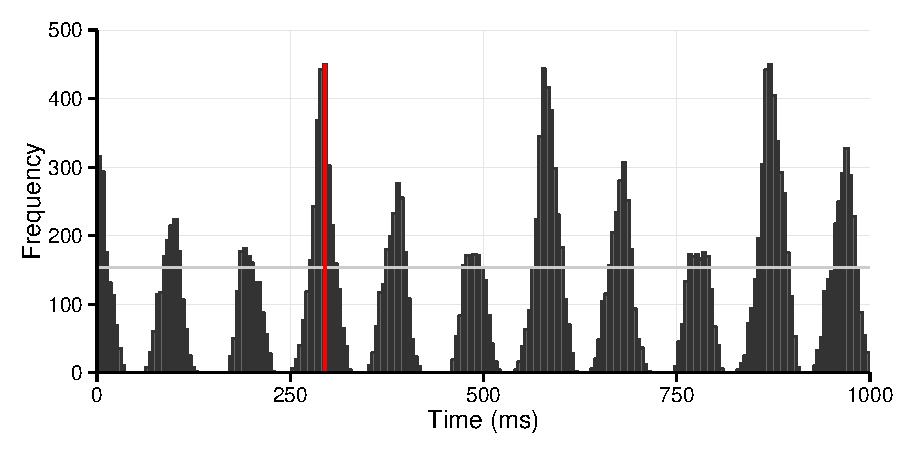
\includegraphics[width=0.8\textwidth]{figures/malawi/rttbin.pdf}
  \caption{$H(t)$ for flow displayed in Figure \ref{fig:hostlimited}. The horizontal line delimits $\overline{H}$ while the highlighted bin denotes the bidirectional RTT estimate.\label{fig:histogram}}
\end{figure}

%
% Explain why did we use FFT
%
The algorithmic recovery of $T$ from $H(t)$ presents additional challenges. 
In particular, $H(t)$ may include a large number of \ac{RTT} multiples, and a peak will be found for all of them. 
Crucially, all these peaks may be of comparable magnitude, complicating the task of selecting a single peak.
Moreover, these peaks need not be very pronounced, with histogram bins in close proximity of the peaks have very similar values as the peak itself. 
As such, taking \ac{RTT} candidates directly from $H(t)$ may result in a large set of similarly-valued bins situated around a peaks at multiples of the \ac{RTT}. 

Three recovery algorithms for $T$ are attempted.
First, as a baseline, the highest peak in $H(t)$ is selected as a candidate for $T$. 
In addition, expanding upon the work of Qian et. al. \cite{Qian:2009p429} a frequency-domain representation of $H(t)$ is used to identify $T$. 
This is done by selecting the highest peak of $|\hat{H}(\omega)|^2$, the \emph{energy spectral density} of $H(t)$ (i.e. the norm squared of the Fourier transform of $H(t)$). 
Finally, a custom utility-based technique that operates directly on $H(t)$ is proposed which achieves superior performance to both of the aforementioned methods.

%\subsubsection{FFT-Based RTT Recovery}
%We extract periodicity information from $H(t)$ by looking at $\hat{H}(\omega)$, the \emph{energy spectral density} of $H(t)$. Formally, $\hat{H}(\omega)$ is defined as the norm squared of the Fourier transform of $H(t)$, so that $\hat{H}(\omega) = |\mathcal{F}(H(t))|^2$. Using $\hat{H}(\omega)$ markedly improves the quality of our RTT estimation because the frequency peak corresponding to the RTT usually accounts for a much larger proportion of the total frequency domain energy than other peaks in $\hat{H}(\omega)$, leading to a much simpler discrimination of the true RTT. However, due to RTT changing during the lifetime of a flow, and also due to the expected noise associated with real-life data sources, $\hat{H}(\omega)$ can also occasionally include large peaks at frequencies unrelated to the RTT. In order to filter these out, we take a set of 10 frequency candidates from $\hat{H}(\omega)$, and use their associated periods as RTT candidates in our flow reconstruction algorithm (see Section \ref{
%subsection:malawi:flightAggregation}). We then select that RTT candidate which exhibits the smallest error, that is, that one which yields closest agreement with observed data.

%
% Algorithmic hacks
%
%To streamline our algorithm for streaming use, we use the following heuristics and approximations. Firstly, we define a range $[T_{\min}, T_{\max}]$ representing the range over which we find the RTT values of interest. Then, for each packet $p_j$, we build a subset $\mathcal{T}_j'$ of $\mathcal{T}_j$ by including all values of $t_j - t_k < T_{\max}$. We then generate $\mathcal{T}' = \cup_j \mathcal{T}_j'$ and approximate $H(t)$ by considering a histogram of the values in $\mathcal{T}'$. As usual, we do this by counting the frequency with which its values are observed in the ranges $[0,\tau)$, $[\tau, 2\tau)$, $[2\tau, 3\tau), \ldots$ where $\tau$ is the time resolution required. 


\subsubsection{Utility-Based RTT Recovery}
\label{sect:utilityBasedRecovery}

This method relies not on the identification of periodicities, but on explicitly matching experimentally found signatures. 
To this end, we consider the peaks of $H(t)$, which are then considered RTT candidates.  
However, trivial discriminators (such as simply selecting the highest peak) are not reliable. 
In this case, it was found experimentally that repeatable peaks and troughs also occur at multiples and sub-multiples of $T$, with the most important ones being $\frac{T}{3}$, $\frac{T}{2}$, $T$ and $2T$. 
We design this detection algorithm around the idea that a given pattern of peaks and troughs can identify $T$.

If we define $\overline{H}$ as the mean height of $H(t)$, we can define a per-peak utility function $p(t)$ so that 
\begin{equation*}
p(t) = 1.0 - \exp\left(-2.0 \left(\frac{H(t)}{\overline{H}}\right)\right) \mbox{.}
\end{equation*}
This function has several advantageous properties: it is 0 if $H(t)$ is zero, 1
if $H(t)$ is infinite, and $0.5$ if $H(t) = \overline{H}$.  In other
words it is a measure of the \emph{peakiness} of the data, with $p=1$ identifying
an infinitely high peak, $p=0$ identifying an empty histogram bin (trough), and $p=\frac{1}{2}$ 
implying that $H(t)$ is of exactly average height at that point. We can then score each candidate using the following utility function:
$$
P(t) = 1.5 p(t) + p(2t) - p\left(\frac{t}{2}\right) - p\left(\frac{t}{3}\right).
$$
That is, the candidate RTT $t$ scores highly if it is itself a peak, if it has a peak
at a multiple $2t$, and if it also manifests troughs at submultiples $\frac{T}{2}$ and $\frac{T}{3}$.
The factor of 1.5 was added after observations
showed that the peak at $T$ was the most important factor in determining
whether a candidate was the true RTT. Similarly, additional multiples and submultiples 
were excluded as they showed very limited discriminating power experimentally.

\begin{figure}
  \centering
  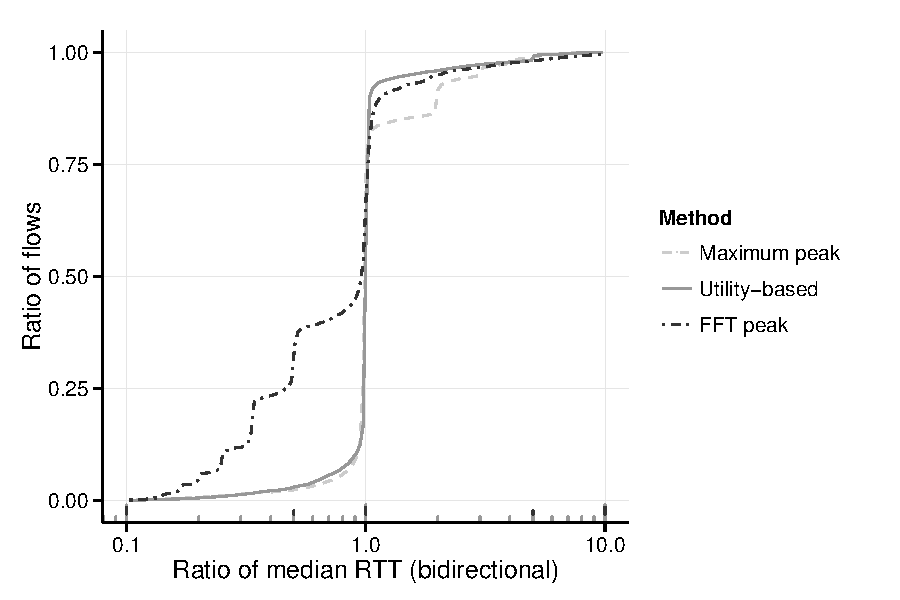
\includegraphics[width=0.8\textwidth]{figures/malawi/rttcomp.pdf}
  \caption{Accuracy of RTT estimator when compared to the median value of bidirectional estimate.}
\end{figure}

\subsubsection{Comparing RTT Recovery Algorithms}
\label{sect:comparingRecoveryAlgos}
As described in Section \ref{subsection:malawi:PeriodicEnhancement}, $H(t)$ is calculated in such a way that RTT periodicity is amplified. 
This means that FFT-based techniques could potentially perform better on $H(t)$ than on the packet stream with no pre-processing. 
However, this is complicated not only because $H(t)$ contains periodicities at multiples of $T$, but also discontinuities that generate harmonics at frequency multiples of the RTT fundamental. 
Hence, although the FFT $|\hat{H}(\omega)|$ of $H(t)$ is much cleaner than that of the packet interarrival time series on its own, its maximum peak rarely coincides exactly with the RTT clock (this corroborates reports by Qian et al \cite{Qian:2009p429}). 
Thus, applying the FFT leads to another \emph{peak detection problem} in which the RTT fundamental needs to be extricated from its harmonics and sub-harmonics. 
The trivial solution to this problem, the application of a bandpass filter around the RTT frequency, is of course unfeasible because the bandwidth and 
centring of such a filter depend on the RTT which is itself unknown.
The utility-based algorithm described in Section \ref{sect:utilityBasedRecovery} can hence be applied in either the time domain or the frequency domain; we chose to do it on the former on the interest of expediency and lower computational cost.

\newcommand{\RTTHeader}{Below & Above}
\newcommand{\SmallFlowName}{\textless 10MB}
\newcommand{\LargeFlowName}{\textgreater 10MB} 
\begin{table}
\footnotesize
\centering
\begin{tabular}{ p{1.5cm} p{1.2cm} p{0cm} p{.6cm}p{.6cm} p{0cm} p{.6cm}p{.6cm}}
& & & \multicolumn{2}{c}{Peak} & & \multicolumn{2}{c}{Utility-based} \\
\cline{4-5} \cline{7-8}
& Flow size & & \RTTHeader & & \RTTHeader \\
\cline{4-5} \cline{7-8} 
\multirow{2}{*}{Receiver side}  & \SmallFlowName && 4.31 & 9.13 && 4.58 & 6.35
\\ 
                                & \LargeFlowName && 6.72 & 6.43 & 4.97 & 5.33
\\
\multirow{2}{*}{Sender side}    & \SmallFlowName && 2.94 & 8.37 && 3.29 & 4.80
\\
                                & \LargeFlowName && 6.41 & 9.06 & 5.40 & 11.06
\\
\end{tabular}
\caption{\label{table:rttRecovery}Performance of RTT recovery algorithms}
\vspace{-3mm}
\end{table}

The performance of the analysed RTT recovery mechanisms is presented in Table \ref{table:rttRecovery}, that shows the percentage of total flows below and above the RTT range given by the bidirectional estimates.
We separate things for \emph{inbound} traffic (where we are positioned at the receiver side) and \emph{outbound} traffic (where we are positioned at the sender side). The utility-based algorithm is particularly useful to address RTT underestimation for flows over 10MB in size, which is our main objective since precisely that kind of estimation error would interfere with our ability to correctly decouple application behaviour from RTT-scale dynamics.


%For the most part, the utility based method improves on underestimation, which is our main objective since that would interfere with our flight reconstruction (i.e. generate lots of gaps).
%The exception (kind of) is traffic from the sender side, which in our training set (one week per year), had quite a lot of host limited traffic (paced out, no signal to recover).
%In this case, not a problem, since if the flow is long enough multiples of the RTT will still reveal host limitation, but will give us a smaller window..


\subsection{Flow Classification}
\label{subsection:malawi:flightAggregation}

One fundamental precondition to decouple the influence that network loss, host configuration and TCP behaviour has on the throughput experienced by a flow is the reconstruction of the congestion window behaviour of TCP flows on the basis of observed data. 
Unfortunately, the congestion window value is internal to the sender's TCP state machine and may not manifest itself in the absence of sufficient data from the application layer. 
A more easily observed quantity which serves as a reasonable proxy for the congestion window is the number of unacknowledged bytes in flight, henceforth referred to as the \textit{flight size}, which can be derived given an accurate estimate of the end-to-end delay.
The evolution of both flight size and RTT can in turn be used to ascertain to what extent throughput is regulated by limitations imposed at different layers of the networking stack.

% definitions
Given a candidate RTT, we can aggregate a stream of packets with arrival times $t_1, t_2, \ldots$ into a stream of \emph{flights}. 
Intuitively, a flight is a clustered subset of a TCP flow which exhibits its own temporal coherence; alternatively, it can be though of as a series of consecutive packets that were (roughly) generated by the sender as a response to the same protocol operation. 
A flight $f_i$ that begins
with the $j$th packet and ends with the $k$th is defined to have a \emph{total flight time} $\tau_i = t_{k+1} - t_j$. 
The algorithmic selection of initial and final packets in such a way that the resulting flights are indicative of TCP behaviour remains an open problem. 
Since we assume that the RTT provides a natural time frame for the operations of TCP, in the algorithm presented in this work, given an initial packet $\pi_j$ and an RTT estimate $T$, the $k$th (and final) packet is selected to minimise \emph{the flight time error} $e_i = |T - \tau_i|$. 
This mechanism follows closely the methodology described in \cite{Zhang:2002p85}, with the exception that we do not attempt to define flights as being both adjacent and disjoint; rather, we decompose flows into a stream of potentially overlapping flights. 
This helps the algorithm mitigate the deleterious effects of small deviations in the estimated RTT, which alters the properties of each flight. 
Furthermore, since the flight size is continuous in time, it makes little sense to restrict ourselves to a single sample per round trip time.

Having obtained flight information from each flow, we next consider what is the predominant factor that affects its throughput. 
Within the context of TCP, we classify flows as being artificially constrained by three distinct processes: \emph{application pacing}, \emph{host limited} and \emph{receiver shaping}.

\begin{figure}
\centering
  \centering
  \begin{subfigure}{1.0\linewidth}
    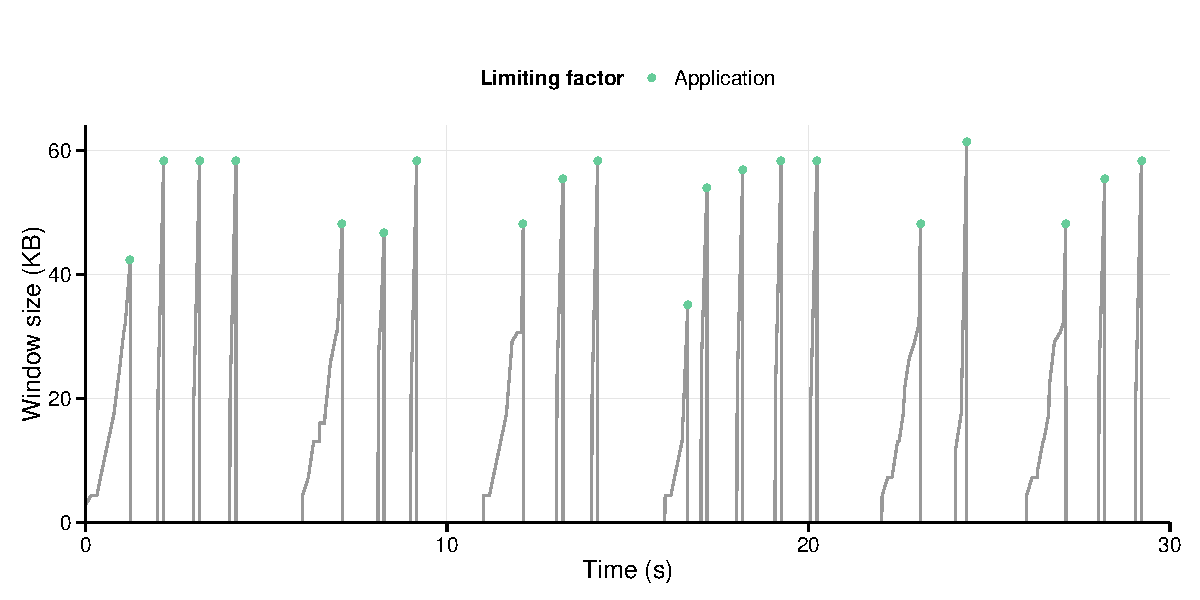
\includegraphics[width=1.0\textwidth]{figures/malawi/youtube.pdf}
    \caption{Application paced. \label{fig:youtube}}
  \end{subfigure}\\
  \begin{subfigure}{1.0\linewidth}
    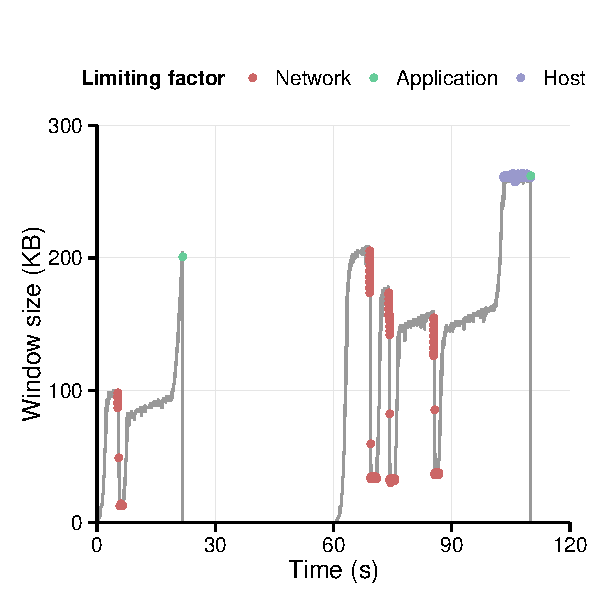
\includegraphics[width=1.0\textwidth]{figures/malawi/hostflow.pdf}
    \caption{Partially host limited. \label{fig:hostlimited}}
  \end{subfigure}\\
  \begin{subfigure}{1.0\linewidth}
    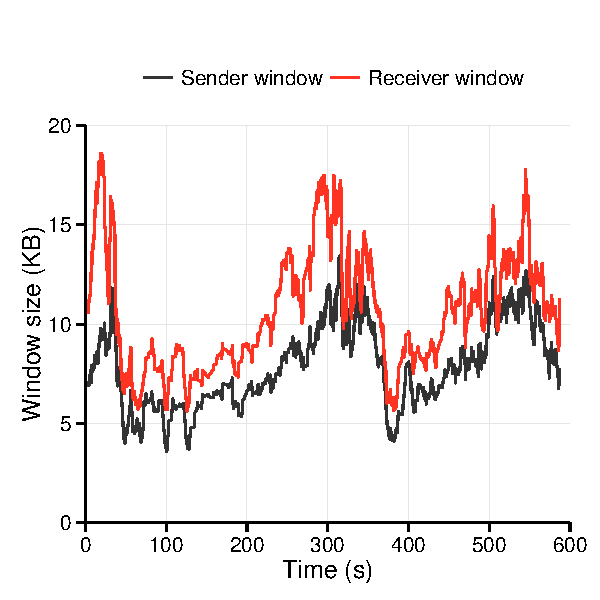
\includegraphics[width=1.0\textwidth]{figures/malawi/awnd.pdf}
    \caption{Receiver shaped. \label{fig:awnd}}
  \end{subfigure}
  \caption{Flight size over time for flows affected by different artificial constraints. \label{fig:kindsOfFlowEffect}}
\end{figure}


\subsubsection{Application Paced Flows}
\label{sssec:app}

A flow whose throughput decreases because it has no outstanding data to send is temporarily limited by the application. 
Flights can be identified as being \emph{application limited} if terminated with a packet smaller than the maximum segment size (MSS) and followed by an inter-arrival time greater than the RTT, as consistent with \cite{Zhang:2002p85}. 
The underlying reason for this defintion is that most TCP implementations will wait some time for subsequent bytes to be written to the socket if the next packet to be sent is smaller than the MSS, unless the TCP\_NODELAY option is set \cite{nagle1984rfc}.

A flow with \emph{application limited} flights however is not necessarily \emph{application paced}. In practice, all flows for which the final packet is observed contain at least one such flight.
For the purposes of our work, we are focused on identifying cases in which throughput is predominantly determined by application behaviour.
One such example is illustrated in figure \ref{fig:youtube}, in which a stream is delivered by periodically writing blocks to the sending socket.
The resulting network-level behaviour is distinct from traditional congestion control: short bursts are interspersed with protracted silence.
Application limited flights, which terminate on non-MSS packets, are highlighted at the end of each burst.

This behaviour is in stark contrast to that exhibited in figure \ref{fig:hostlimited}, where distinct transfers are multiplexed on top of a single transport association over time.
From the perspective of the network, there is little to distinguish the behaviour of such traffic from independent TCP flows.
Application paced connections such as Youtube traffic however exhibit a degree of regularity which can potentially be exploited by the network in predicting demand or smoothing bursts.

In order to identify such recurring behaviour, we identify flows as being \emph{application paced} if the period between bursts terminated by \emph{application limited flights} is consistently under 10 seconds and the standard deviation of the intermediate pauses is under one second.
This definition in particular purposely ignores flows which exhibit long silence periods due to user interaction, and follows closely the behaviour historically associated to Youtube streaming in particular.

\subsubsection{Host Limited Flows}
\label{sssec:host}

Given sufficient bandwidth and traffic to send, a flow may encounter local constraints at either end-host which cap its throughput. 
For instance, the buffer space allocated on both the sender and receiver side is often pre-configured, and it is common practice to tune these values down on popular servers and managed infrastructure in a bid to conserve memory or bandwidth.
A receiver is also limited in the window size it can announce to the remote sender; if the windowscale option \cite{jacobson1992tcp} is not negotiated during the TCP handshake, the advertised window cannot exceed 64KB.

In both cases, a local decision by either host can determine the upper bound of the flow rate.
These \emph{host limited} cases are characterised by a constant window size over time.
The methodology described for flight aggregation at the beginning of this section typically generates a large number of flights, representing many likely combinations given a base RTT estimate.
In order to identify the flat-lined behaviour of a host limited flow, we first filter the flight stream to remove some of the uncertainty derived from small fluctuations in the RTT.
We then select the maximum flight size observed for each RTT interval, and declare a sequence of flights to be host limited if the same maximum was observed over six consecutive RTTs (this is twice the period suggested in \cite{Zhang:2002p85}).
In practice, increasing the period over which the maximum window size is tracked allows us to more accurately discern between host limited behaviour and more conservative bandwidth probing, such as that performed during the convex phase of TCP CUBIC \cite{Ha:2008p471}.

A flow may be host limited for only brief periods of its lifetime, as illustrated in figure \ref{fig:hostlimited}.
To filter out such cases where host limitations are not the predominant factor in defining flow throughput, we further enforce that in addition to host-limited flights, the average window size must over a flow lifetime should be within 10\% of the inferred host limit, which is not the case in figure \ref{fig:hostlimited}.

In practice, flows can exhibit both application pacing and host limitations, with bursts being sent at a capped window size followed by application pauses.
In such cases, a flow will still be classified as being \emph{application paced} if it meets the requirements set out in the previous section, as doing so provides evidence that it controls throughput in spite of the degraded performance provided further down the stack. 
This line of reasoning applies equally to the occurrence of sporadic loss; so long as block delivery is ensured within the timeframe dictated by the application, it remains in control.

\subsubsection{Receiver Shaped Flows}
\label{sssec:rec}

A flow which is neither \emph{application paced} or \emph{host limited} can still be artificially constrained by flow control (rather than by congestion control).
Traditionally, in TCP the sender is responsible for regulating throughput. 
However, the receiver can also shape throughput by manipulating the \emph{advertised window} announced on every acknowledgement.
Such receiver-window auto-tuning has been available on Windows operating systems since Vista \cite{vistaReceiveWindow}, and can also be leveraged by middleboxes in order to throttle inbound traffic \cite{appEx}.

In order to evaluate the potential impact of such behaviour, we further propose a heuristic to identify receiver-shaped traffic.
For flows in which both directions of traffic are observed it is possible to correlate the evolution of the advertised window with the size of reconstructed flights.
Figure \ref{fig:awnd} displays an example of a receiver-shaped connection, in this case throttled by an intermediate middlebox.
Since the advertised window may be fluctuating, it is not always obvious which of the many updates were effectively applied by the sender as successive values supersede each other.
An example of a reconstructed flow which is subjected to receiver shaping is displayed in Figure \ref{fig:awnd}.

For flows in which both directions are observed, it is possible to classify flights as being receiver-shaped if there is a statistically significant correlation between the advertised window size and the maximum flight size observed.
Harnessing the stream filtering used in detecting host limited behaviour, we perform such analysis over a sliding window of 10 RTT intervals.
A flight is flagged as being receiver shaped if the correlation between receiver window and flight size is statistically significant; a flow is considered to be predominantly receiver shaped if over half of its flights are flagged as such.
We do not perform this covariance analysis on flights which contain out-of-order or retransmitted packets. 
In these cases, both the receiver and sender window sizes are correlated \emph{by definition}. 
In the former case, the receiver buffer will temporarily fill expecting the next packet in sequence, in the latter case, TCP will reduce its window.

Given that receiver shaping classification requires correlating information in both directions of a TCP connection, it will come as no surprise that the absence of the reverse path can introduce false positives into our measurements. 
This happens because any given flow might be receiver shaped in such a manner that the heuristic erroneously attributes its behaviour to host limitations. 
In the absence of additional evidence, this misclassification is difficult to detect explicitly. 
Instead, we calculate the ratio of receiver shaped flows which would have been incorrectly identified if the reverse path were not observed. 
This error rate can then be used to evaluate the accuracy of classifier results.

\section{Macroscopic traffic trends}
\label{section:malawi:macro}

\begin{figure}
  \centering
  \begin{subfigure}[b]{1.0\linewidth}
  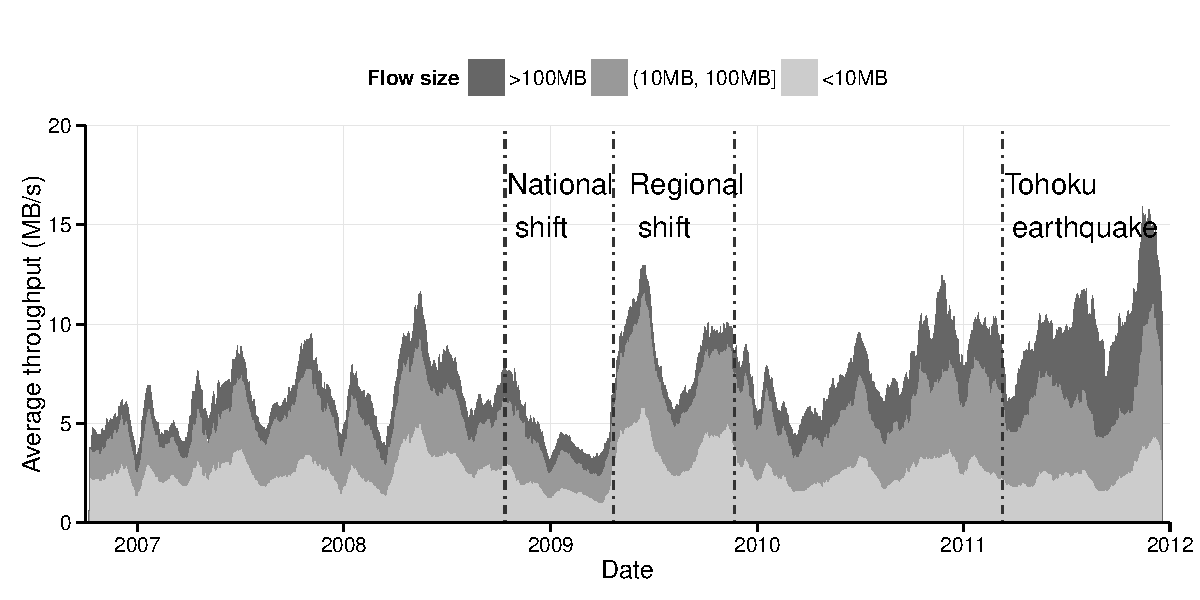
\includegraphics[width=0.9\textwidth]{figures/malawi/tput}
  \caption{Mean throughput}
  \end{subfigure}
  \begin{subfigure}[b]{1.0\linewidth}
  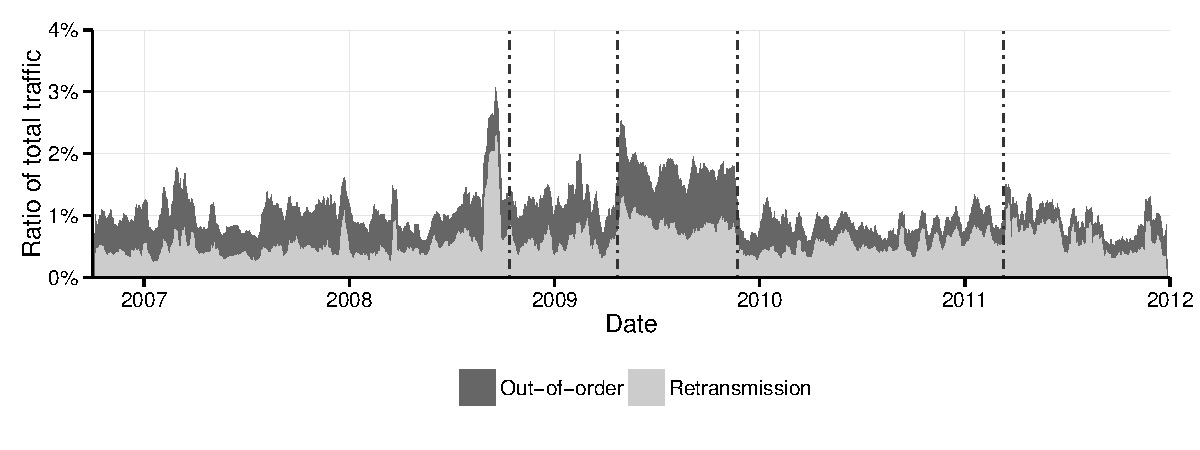
\includegraphics[width=0.9\textwidth]{figures/malawi/losses}
  \caption{Mean loss rate}
  \end{subfigure}
  \caption{Longitudinal evolution of inbound traffic.}\label{fig:MAWI}
\end{figure}

Over a five year period, changes in routing and application popularity have continually redefined the nature of traffic under observation.
This section provides a macroscopic view of these shifting trends. Figure \ref{fig:MAWI} displays the average throughput and loss ratio, calculated for TCP traffic only, smoothed on a weekly basis. 
Two routing changes internal to WIDE had significant impact on overall traffic, and are consequently highlighted.
The first, performed towards the end of 2008, diverted most of the inbound traffic from \emph{national} sources away from the monitored transit link, resulting in a reduction of traffic.
This event was preceded by increased congestion downstream from the monitoring point.
The second, in early 2009, saw a significant increase in \emph{regional} traffic from Asian neighbours, and was reverted approximately six months later. 
During this period aggregate end-to-end loss rates increased as a result.
While this is mostly due to the higher proportion of upstream congestion for traffic from Taiwan and China in particular, most traffic was adversely affected by the increased utilisation, suggesting that the transit link itself may have been a bottleneck during this period.
Finally, the impact of the Tohuku earthquake resulted in a noticeable break in demand coinciding with the start of the Japanese fiscal year in April, in which traffic traditionally ramps up.

\subsection{Geographic distribution}

\begin{table}\footnotesize
\centering
    \begin{tabular}{  
@{}
$>{\scshape}p{3.0cm}
^r
^r
^r
^r
^r@{\hskip 1.0cm}
^r
^r
^r
^r
^r
@{}
}
\toprule
\rowstyle{\scshape\bfseries}
\multirow{2}{*}{\parbox[][0.7cm][b]{3.0cm}{Country}} & 
\multicolumn{5}{c}{\scshape\bfseries{Outbound traffic (\%)\hspace*{0.45cm}}} & 
\multicolumn{5}{c}{\scshape\bfseries{Inbound traffic (\%)}} \\
\cmidrule(r{1.0cm}){2-6} \cmidrule{7-11}
\addlinespace[-0.6em] \rowstyle{\scriptsize\scshape}
 & 2007 & 2008 & 2009 & 2010 & 2011 & 2007 & 2008 & 2009 & 2010 & 2011 \\
\midrule

        United States & 27.3 & 31.3 & 29.3 & 36.4 & 35.7 & 45.7 & 41.5 & 53.3 & 65.1 & 67.1
\\
        \scriptsize{ California } & \scriptsize{ 39.0 } & \scriptsize{ 61.8 } & \scriptsize{ 63.5 } & \scriptsize{ 53.8 } & \scriptsize{ 50.6 } & \scriptsize{ 55.7 } & \scriptsize{ 47.9 } & \scriptsize{ 46.7 } & \scriptsize{ 24.9 } & \scriptsize{ 34.9 }\\\scriptsize{ Texas } & \scriptsize{  5.8 } & \scriptsize{  4.3 } & \scriptsize{  4.1 } & \scriptsize{  2.4 } & \scriptsize{ 13.9 } & \scriptsize{  7.0 } & \scriptsize{ 12.0 } & \scriptsize{  5.8 } & \scriptsize{  7.1 } & \scriptsize{  5.6 }\\\scriptsize{ Colorado } & \scriptsize{  1.9 } & \scriptsize{  1.2 } & \scriptsize{  0.6 } & \scriptsize{  8.5 } & \scriptsize{  2.8 } & \scriptsize{  4.9 } & \scriptsize{  6.0 } & \scriptsize{  5.9 } & \scriptsize{  9.7 } & \scriptsize{  5.8 }\\\scriptsize{ Virginia } & \scriptsize{  1.9 } & \scriptsize{  1.0 } & \scriptsize{  0.8 } & \scriptsize{  0.4 } & \scriptsize{  0.6 } & \scriptsize{  1.2 } & \scriptsize{  3.0 } & \scriptsize{ 14.1 } & \scriptsize{ 13.1 } & \scriptsize{  8.3 }\\\scriptsize{ Washington } & \scriptsize{  4.0 } & \scriptsize{  2.9 } & \scriptsize{  3.5 } & \scriptsize{  6.1 } & \scriptsize{  6.6 } & \scriptsize{  0.9 } & \scriptsize{  5.7 } & \scriptsize{  3.5 } & \scriptsize{  3.0 } & \scriptsize{  2.0 }\\\scriptsize{ New Jersey } & \scriptsize{  2.8 } & \scriptsize{  1.5 } & \scriptsize{  0.7 } & \scriptsize{  1.1 } & \scriptsize{  1.9 } & \scriptsize{  1.0 } & \scriptsize{  1.8 } & \scriptsize{  1.6 } & \scriptsize{  4.9 } & \scriptsize{ 13.6 }\\\scriptsize{ Massachusetts } & \scriptsize{  1.6 } & \scriptsize{  1.1 } & \scriptsize{  0.9 } & \scriptsize{  6.1 } & \scriptsize{  4.9 } & \scriptsize{  5.4 } & \scriptsize{  2.1 } & \scriptsize{  1.8 } & \scriptsize{  1.6 } & \scriptsize{  2.0 }\\\scriptsize{ Florida } & \scriptsize{  3.1 } & \scriptsize{  2.3 } & \scriptsize{  1.3 } & \scriptsize{  1.1 } & \scriptsize{  0.9 } & \scriptsize{  1.0 } & \scriptsize{  0.4 } & \scriptsize{  0.4 } & \scriptsize{  8.5 } & \scriptsize{  7.9 }
\\
        Japan & 11.6 & 15.4 & 17.7 & 16.7 & 16.1 & 33.8 & 32.2 &  7.3 & 8.1 & 11.5\\China &  7.9 & 20.5 & 17.8 & 10.3 &  5.9 &  2.5 &  5.3 &  6.3 & 4.6 &  3.1\\Korea, Republic of &  5.3 &  1.3 &  2.1 &  7.8 & 23.8 &  4.7 &  5.1 &  3.2 & 1.1 &  0.5\\Germany &  2.2 &  1.7 &  1.6 &  1.0 &  0.6 &  3.0 &  6.1 &  5.3 & 5.5 &  1.4\\Taiwan &  2.7 &  1.3 &  4.0 &  3.6 &  2.7 &  0.8 &  0.9 & 10.9 & 0.9 &  0.4\\Netherlands &  0.4 &  0.4 &  0.5 &  0.3 &  0.4 &  0.9 &  1.0 &  4.1 & 6.2 &  6.9\\India &  2.8 &  3.3 &  4.8 &  3.3 &  2.0 &  0.3 &  0.1 &  0.0 & 0.2 &  0.0\\France &  1.2 &  1.1 &  0.9 &  0.9 &  0.9 &  1.6 &  1.2 &  2.6 & 3.4 &  1.7\\United Kingdom &  1.1 &  1.0 &  1.0 &  0.9 &  0.7 &  2.5 &  2.2 &  1.6 & 1.3 &  1.3
\\
    \end{tabular}
  \caption{Percentage of inbound and outbound traffic by country\label{table:dest}. U.S. state values are relative to total national traffic.}
\end{table}



These changes are both visible in the geographic distribution of inbound traffic over time, shown in table \ref{table:dest}.
Prior to 2009, a significant proportion of transit traffic originated from within Japan. Over time, however, the ratio of traffic from Asia has been reduced. While this may foreshadow an increased concentration of traffic from the United States, it should primarily be viewed as a reflection of routing policy, with regional traffic being diverted to alternate routes as Japan became increasingly interconnected to its neighbours.


Further geographic shifts are apparent when breaking down US traffic by state.
The proportion of traffic originating from California has decreased over time, dropping from 55\% of total US traffic in 2007 to only 35\% in 2011.
In its place, a larger set of states have emerged as content providers, with New Jersey, Florida and Virginia contributing over a quarter of all traffic originating within the US by 2011.

%tip

Table \ref{table:dest} shows the geographic distribution of both inbound and outbound traffic since 2007. The majority of traffic flows to and from the United States, which has increased its share of bandwidth in either direction over the past five years. The proportion of traffic flowing from the United States is particularly high, accounting for almost 70\% of inbound traffic in 2011. While this may foreshadow an increased concentration of traffic within the United States, it should first be viewed as a reflection of routing policy, as regional traffic has been increasingly diverted to alternate routes. Inbound traffic from Japan, China, Korea and Taiwan have all been on the wane over the past five years as Japan has become increasingly interconnected to its neighbours. Of particular importance is the routing change at the end of 2008, which resulted in a sharp drop in inbound traffic from within Japan, with a net effect easily discernable in figure \ref{fig:inout}. This event had a profound influence in shaping not only the distribution of traffic, but also overall loss and delay as we shall observe in sections \ref{sec:delay} and \ref{sec:loss}.

A further point of interest is the breakdown of traffic from the U.S. by state. The overall increase in volume at a national level has broken the hegemony of California, which saw its overall share of inbound traffic fall from 60\% in 2007 to just under 40\% by 2011. In its place a larger set of states have emerged as content providers. Not listed are New Jersey, Florida and Virginia, which all saw sharp rises in 2011 to provide 35\% of all traffic from the U.S towards WIDE.
    
In the outbound direction, the geographic distrubtion of traffic is less skewed, with a greater proportion of traffic flowing towards Japan and China in particular. Due to a change in routing towards the end of 2010, traffic to Korea increases dramatically. In 2011, 12.7\% of all outbound traffic was destined to Korea Telecom alone. European destinations overall have a small proportion of outgoing traffic, which appears to be shrinking over time. The most significant factor for the discrepancy between inbound and outbound traffic for Europe as a whole is the timezone difference, as traffic is measured at 05:00GMT. This however does not account for why outbound traffic overall has been falling. Since most outbound traffic towards Europe at the time of measurement is likely to be scheduled transfers with no human intervention, a plausible explanation for this trend is the gradual shift away from file-sharing using peer-to-peer applications. This is further corroborated by the rise of hosting solutions which facilitate filesharing such as MediaFire, as shall become evident when analyzing the breakdown of traffic by AS.


\


\subsection{\acs{AS}-level distribution}
\begin{figure}
    \centering
    \begin{subfigure}[b]{0.5\linewidth}
        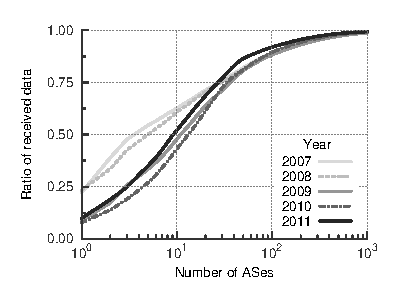
\includegraphics{figures/malawi/asn_cdf_in}
        \caption{Inbound}
    \end{subfigure}%
    \begin{subfigure}[b]{0.5\linewidth}
        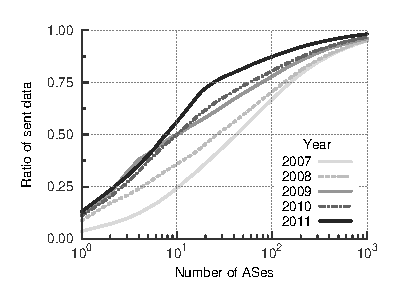
\includegraphics{figures/malawi/asn_cdf_out}
        \caption{Outbound}
    \end{subfigure}%
    \caption{CDF of inbound data by AS. \label{fig:ecdf_asn_from}}
\end{figure}


%\begin{table*}\scriptsize
%\centering
%\subfloat[2007]{
    %\begin{tabular}{
@{}
$>{\raggedleft}p{0.6cm}
^>{\scshape}p{2.25cm}
^>{\raggedleft\arraybackslash}p{0.6cm}
@{}
}
\toprule
\rowstyle{\scshape\bfseries}
\acs{ASN} & \acs{AS} name &
\% \\
\midrule

    %\input{data/malawi/asn2007.tex}
    %\end{tabular} % closes asnheader.tex tabular environment
    %}
%\subfloat[2009]{
    %\begin{tabular}{
@{}
$>{\raggedleft}p{0.6cm}
^>{\scshape}p{2.25cm}
^>{\raggedleft\arraybackslash}p{0.6cm}
@{}
}
\toprule
\rowstyle{\scshape\bfseries}
\acs{ASN} & \acs{AS} name &
\% \\
\midrule

    %\input{data/malawi/asn2009.tex}
    %\end{tabular} % closes asnheader.tex tabular environment
%}
%\subfloat[2011]{
    %\begin{tabular}{
@{}
$>{\raggedleft}p{0.6cm}
^>{\scshape}p{2.25cm}
^>{\raggedleft\arraybackslash}p{0.6cm}
@{}
}
\toprule
\rowstyle{\scshape\bfseries}
\acs{ASN} & \acs{AS} name &
\% \\
\midrule

    %\input{data/malawi/asn2011.tex}
    %\end{tabular} % closes asnheader.tex tabular environment
%}
%\caption{
    %\label{table:topASin}
    %Top 10 ASes for inbound traffic by year. Additionally listed is the ratio of aggregate end-to-end loss.}
%\vspace{-3mm}
%\end{table*}


These large-scale changes are a natural outcome of content consolidation. This is most apparent at the AS level, where a direct mapping to a commercial entity is forthcoming.
Figure \ref{fig:ecdf_asn_from} shows the cumulative distribution of inbound traffic by AS, while table \ref{table:topASin} lists the top ten AS by traffic volume for 2007, 2009 and 2011.
While in 2007 traffic was already consolidated across a small set of ASes, a significant portion of transit traffic was Asian: most traffic from NTT and Limelight originated from within Japan. Such traffic has gradually been pushed away from transit by 2011.
Large carriers such as Cogent, Level3, Hanaro, China Telecom have also seen their importance diluted by ASes known to harbour one-click hosting services such as Choopa, Webazilla, WZ Communications, Carpathia and LeaseWeb.
Many of the hosted websites facilitate the distribution of copyrighted content, and as such are not capable of growing large enough to expand beyond hosted infrastructure without risking prosecution.
% overall summary: content consolidation, delay, etc
Overall, the observed traffic patterns match the insights provided by Labovitz et al. on the changing nature of interdomain traffic in \cite{Labovitz:2010p175}.
The implications for transit traffic from an Asian perspective is less intuitive: with the increased adoption of content delivery networks and internet exchanges points, more transit traffic is being retrieved from further away as content in the US shifts east.


%tip
It has been widely noted that inter-domain traffic has significantly changed over the past decade, with an increasing proportion of traffic flowing to and from a dwindling set of both large content providers and consumer networks. 
This shift carries potentially significant ramifications for network operators. 
Content consolidation provides opportunities for network optimization as a wider set of traffic is contained within a smaller set of addresses. 
Improved transport heuristics or dynamic traffic engineering are both feasible solutions under such conditions if designing for the typical case, rather than the worst case \cite{Dukki}.

Traffic consolidation is most apparent at the AS level, where a direct mapping exists to a commercial entity. 
How this translates down to the network layer is less clear. 
We start by investigating how traffic is distributed by both AS and network prefixes for inbound traffic, as shown in figure \ref{fig:ecdf_from}. 
Over the past five years, traffic has remained consistently concentrated in the top 100 ASes, accounting for approximately 90\% of all data received. 
Between 2008 and 2009, traffic to NTT (AS2914) dropped significantly as a wide range of Japanese prefixes were rerouted through a different ingress. 
Additionally, traffic from Limelight ceased to be visible from our measurement point. 
Together, they contributed over 30\% of all inbound traffic in 2007 and 2008. 
This explains the discrepancy in distribution between 2008 and 2009.

For outbound traffic, shown in figure \ref{fig:ecdf_to}a, consolidation has been much more perceptible. 
For the top 10 ASes alone, the proportion of traffic has more than doubled between 2007 and 2011. 
By 2011, the distribution of traffic amongst ASes for inbound and outbound traffic bears a striking similarity. 
The nature of this concentration is markedly different however, as made apparent by the distribution of traffic over network prefixes. 
The one hundred most popular network prefixes contribute 75\% of inbound traffic, yet only account for 50\% of outbound traffic. 
This matches our expectations on the inherent differences between large ISPs, which reflect the heterogeneity of their customer base through addressing, and content providers and CDNs concentrating resources in fewer locations. 



To further highlight this trend we display the top 10 ASes for both inbound and outbound traffic for 2007 and 2011 in tables \ref{table:topASout} and \ref{table:topASin} respectively. For each table we list the number of observed networks - networks belonging to that AS to which traffic was routed to over the entire year - the number of network prefixes which belong to the top 10000 networks and the ratio of traffic. Additionally, we display the values of the latter two values for prefixes with mask values greater than 19.

    For inbound traffic, both large consumer networks and content providers coexist in 2007. Youtube, Limelight, Google, Akamai and AcroNOC all send traffic almost exclusively from smaller address blocks. Additionally, most observed networks are amongst the highest ranked prefixes for inbound traffic, as opposed to large providers like NTT and Cogent, who have a much larger set of address blocks, but many of which do not have significant traffic. By 2011, NTT is the only ranked AS which still exhibits such behaviour for inbound traffic.

    Outbound traffic differs in many respects. Firstly, traffic was much less concentrated in 2007, with top ranked Google receiving a mere 3.6\% of all traffic. The remainder of the list is mostly compromised of large providers receiving most traffic through less specific prefixes. Curiously, NTT displays different patterns between inbound and outbound traffic, with a tendency to send from less specific prefixes, and receive to more specific ones. 

    In 2011 Korean telecom company KIXS exhibits a similar behaviour.  %WHY ??

    In this section we have shown how traffic consolidation has occured at different paces depending on the direction of traffic. Inbound traffic already showed strong signs of concentration in 2007, whereas outbound traffic has become dominated by large consumer networks and regional providers over the past five years. For both cases, traffic has converged towards similar distributions when analyzed by autonomous system, but the impact on routing seems markedly different. We will next focus on how these trends affect end-to-end traffic.


\subsection{Delay}
 
While understanding where traffic flows to and from is of great value at an operational, commercial and often political level, it portrays a small part of a wider picture. 
For end-users it is of less concern where content is being retrieved from or routed through compared to how long it takes.

\begin{figure}
    \centering
    \begin{subfigure}[b]{0.5\linewidth}
        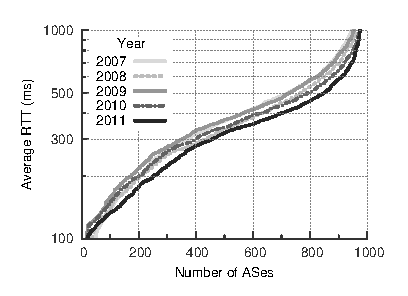
\includegraphics{figures/malawi/rtt_cdf_in}
        \caption{Inbound}
    \end{subfigure}%
    \begin{subfigure}[b]{0.5\linewidth}
        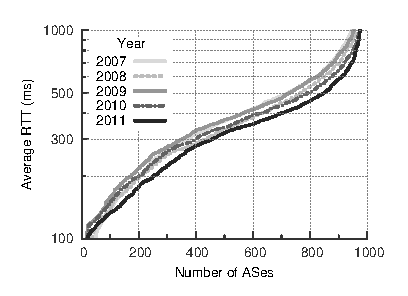
\includegraphics{figures/malawi/rtt_cdf_out}
        \caption{Outbound}
    \end{subfigure}%
    \caption{CDF of RTT by AS. \label{fig:rtt_cdf}}
\end{figure}

\begin{figure}
    \centering
    \begin{subfigure}[b]{0.5\linewidth}
        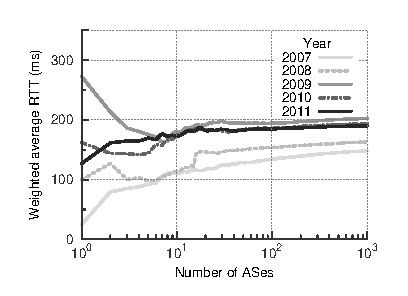
\includegraphics{figures/malawi/rtt_wcdf_in}
        \caption{Inbound}
    \end{subfigure}%
    \begin{subfigure}[b]{0.5\linewidth}
        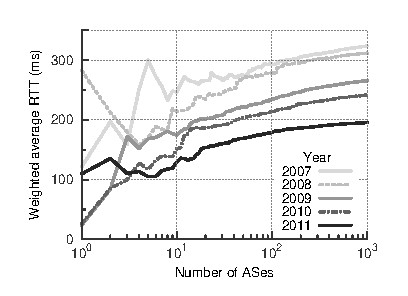
\includegraphics{figures/malawi/rtt_wcdf_out}
        \caption{Outbound}
    \end{subfigure}%
    \caption{CDF of weighted RTT by AS. \label{fig:rtt_wcdf}}
\end{figure}

The respective cumulative distribution functions of delay is display in figure \ref{fig:rtt_ecdf}. As with traffic distributions, the plots once again illustrate the same overall trend in subtly different patterns. Overall, delay has been decreasing over time, with the notable exception of a small segment of inbound traffic for network prefixes, mostly based in Japan, which were rerouted at the end of 2008. The rate at which delay has improved however seems markedly different. 

Comparing plots at the AS granularity, for the top 400 ASes delay has dropped by 20ms between 2009 and 2011 for inbound traffic, while the equivalent decrease for outbound traffic has been closer to 50ms. The absolute values in both cases are still disparate: over 90\% of ASes are reached within a round trip time of approximately 400ms when ranked by inbound traffic, whereas the equivalent value for outbound traffic is almost 200ms higher. This same trend is apparent when looking at delay by network prefix.

For inbound traffic the average RTT is low enough that geographical properties are clearly visible. A first plateau close to 100ms is apparent for traffic to the american west coast, while traffic to european destinations is clustured close to 250ms. Tellingly, this second plateau seems to be receeding in both AS and network plots. When taken in conjunction with the geographic distribution of traffic presented in table \ref{table:dest} this seems to confirm our suspicions that there has indeed been a reduction in the number of sources within Europe. 

A pertinent question at this point is in trying to understand how delay relates to traffic volumes. Given the different nature of stakeholders monopolizing traffic at either end of the spectrum, what can we say about the evolution of delay in either case? To assess this we plot the cumulative distribution of the average RTT weighted by the respective volume of traffic, as shown in \ref{fig:wrtt_ecdf}. In interpreting such plots one should keep in mind that they provide a rough indicator of the average delay to be expected if one were to sample a packet belonging to the top $N$ sources or destinations. As $N$ increases, we will approach the average RTT for all traffic in a given direction.

Inbound traffic by AS highlights and expected rise in delay between 2008 and 2009, as both NTT and Limelight are replaced by more distant sources. However, from 2009 onwards the overall delay is remarkably similar. While the cumulative distribution function of RTT shows improvement in delay at the tail, this results in very little improvement overall as traffic is dominated by a handful of entities.

Focusing on inbound traffic by network prefix not only confirms this, but actually shows that average delay has increased consistently over time.
In this case, the cumulative distribution of delay from \ref{fig:rtt_ecdf}b improved between 2009 and 2011, yet the average weighted RTT increased almost twofold for the top 10 network prefixes over the same period.

Two explanations emerge for this behaviour. The first stems from the changing nature of the traffic we are sampling. While functionally NTT represents the same entity over time, the traffic we observe is very different. As local traffic has increasingly been exchanged over peering links our view of traffic has stretched further afield. To illustrate this, one needs only notice that the average delay towards NTT, the top AS for inbound traffic in both 2007 and 2011, increased by approximately 100ms in figure \ref{fig:wrtt_ecdf}a. This does not represent a degradation in quality of service, but rather a change in where traffic is flowing from within the AS.

A further reason relates to the placement of content. As we had previously shown in \ref{table:dest}, there appears to be a migration of content away from California. Hosting sites such as Lemuria (Hotfile), based in Florida, Mediafire, based in Texas and District of Columbia and Carpathia, based in Virginia, are all contained within the top 20 ASes and have shifted traffic further from locations which had traditionally benefitted from low latency as viewed from Japan.

Analyzing the outbound traffic we seemingly get the opposite effect, with the average weighted RTT for the top 1000 ASes dropping by over 100ms. Once more, there is no single reason which accounts for the entirety of this effect. In 2007 many of the top destination ASes were in developing Asian countries, where infrastructure has improved greatly since. Improvements in routing to countries such as China and Korea have also had a positive net effect. This is visible in figure \ref{fig:rttyearcomp}, where the average RTT aggregated by country is plotted. For clarity, we filter out countries for which RTT estimates are available for less than 50 days in a year. Between 2007 and 2009 most Asian and European countries experience significant improvements in RTT. Those which don't tend to experience lower delays. Between 2009 and 2011 most countries reduce delay below 500ms. 

Finally, many of the very same companies which have had an effect of increasing RTT for inbound traffic, such as Mediafire or Ustream.tv, are also amongst the top destinations of traffic. It is interesting to note that as of 2011, data travelling from the top 1000 AS traffic sources is expected to experience the same latency as data travelling towards the 1000 most popular AS traffic destinations. In 2007, the value was two times higher for outgoing traffic.


\begin{figure}
    \centering
    \begin{subfigure}[b]{0.5\linewidth}
        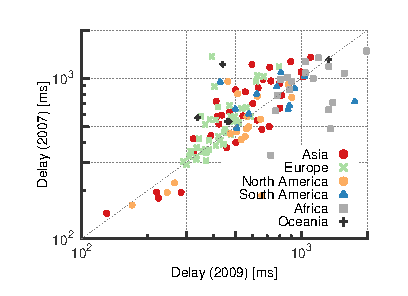
\includegraphics{figures/malawi/rtt_comp_07_09}
        \caption{Inbound}
    \end{subfigure}%
    \begin{subfigure}[b]{0.5\linewidth}
        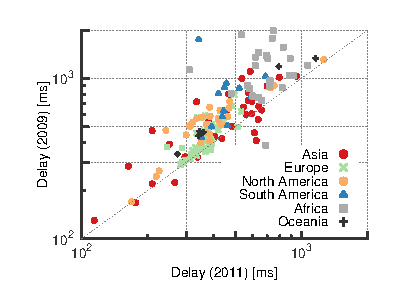
\includegraphics{figures/malawi/rtt_comp_09_11}
        \caption{Outbound}
    \end{subfigure}%
    \caption{CDF of weighted RTT by AS. \label{fig:rtt_comp}}
\end{figure}


\section{Performance Analysis}
%4.1) Balancing between two paths with high loss using fixed time unit
% using only loss-based balance in a simple regime where that works.
% Show how this converges quickly when one path suddenly gains
% background traffic (and hence loss).
%4.2) Balance between several paths with high loss and fixed time unit
% in simple regime where that works.
%4.3) Introduce experiment where equi-path is needed for probing and
% conservative is needed for low loss regime.
%4.4) Introduce experiment where time-scale tuning is needed to get
% good assessment of loss in low traffic regime.

This section evaluates \ac{PREFLEX} through simulation using ns-3 \cite{ns3}. 
Evaluating traditional traffic engineering methods typically involves abstracting traffic as flow aggregates, making large scale network performance analysis tractable.
\ac{PREFLEX} however balances traffic using loss rather than load, and focuses on improving end-user metrics as opposed to minimizing maximum link load.
As such, evaluating the proposed congestion balancer requires simulating end-to-end behaviour of traffic.

\subsection{Methodology}
\label{section:methodology}

Experimental validation is performed using the network topology displayed in figure \ref{fig:topo}. 
The topology links a client domain $C$ to a server domain $S$ through $N$ paths with equal bottlenecks $L_i$, and total bandwidth $B=\sum{L_i}$. 
While a domain is represented as a single entity in figure \ref{fig:topo}, each domain is composed by a traffic generator connected to a router. 
Client $C$ generates $G$ simultaneous \ac{HTTP}-like requests (or ``gets") from $S$ according to a specified distribution, described at the end of this section. 
As traffic flows from $S$ to $C$, the router within $S$ is responsible for balancing traffic over all available paths.

\begin{figure}
    \centering
    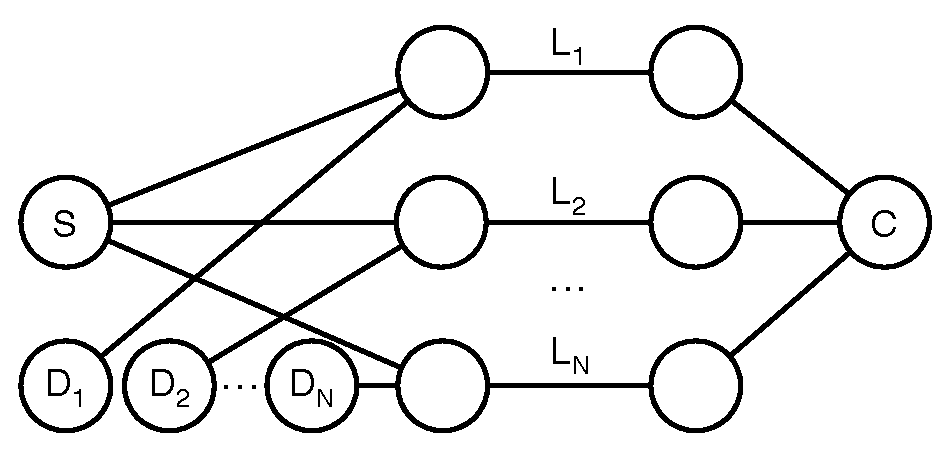
\includegraphics[width=2.5in]{figures/cate/topo}
    \caption{Simulation topology}
    \label{fig:topo}
\end{figure}

Across simulations, as the number of paths increases, total bandwidth $B$ and the number of simultaneous requests $G$ is fixed, providing insight into how efficiently \ac{PREFLEX} balances traffic as the granularity with which it can split traffic becomes coarser.

In order to evaluate how \ac{PREFLEX} shifts traffic in response to loss, additional ``dummy" servers $D_i$ are connected to $C$ through bottleneck link $L_i$.
The simulation runs for time $T$ and is partitioned into $N+2$ intervals starting on $s_i$, in which $s_0$ and $s_{N+1}$ have no traffic to $D_i$. 
Starting at time $s_i$, client $C$ generates $g_i$ requests to $D_i$ according to the same distribution as used to server $S$. 
All requests to $D_i$ end at time $s_{N+1}$. 
Equation \eqref{eq:si} sets the start time $s_i$ for requests to $D_i$ as a function of total simulation time $T$ and number of paths $N$. 
Likewise, equation \eqref{eq:gi} sets the number of simultaneous requests $g_i$ to $D_i$ as a function of $G$, the total number of requests to $S$, and $N$.
\begin{equation}
s_i = T\frac{i}{N+2}
\label{eq:si}
\end{equation}
\begin{equation}
\theta_i = \frac{\frac{1}{N+1-i}}{\sum{\frac{1}{N+1-i}}},  g_i = G\theta_i.
\label{eq:gi}
\end{equation}

Figure \ref{fig:demand} illustrates the number of simultaneous gets from $C$ to $D_i$ for $N=2$ (used in the example shown in figure \ref{fig:two}) and $N=4$. 
Generating cross-traffic in this manner serves two purposes. 
Firstly, $\sum{g_i}=G$, so independently of the number of concurrent paths, the maximum load in the system is $2G$. 
However, as the number of paths increases, the fluctuation in load for each path becomes smaller, stressing the sensitivity with which \ac{PREFLEX} must balance traffic. 
Secondly, the number of requests for each $D_i$ over time is the same. 
Over timescale $T$, equalisation appears to be an acceptable strategy but will however be shown to fail to make efficient use of available capacity. 
This is a fundamental limitation of offline traffic engineering, which is calculated over very long timescales and is unable to adapt as traffic routinely shifts.

\begin{figure}
    \begin{subfigure}[b]{.5\linewidth}
        \centering
        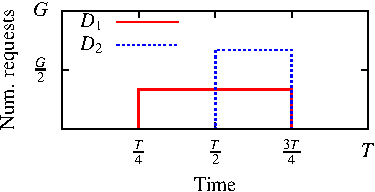
\includegraphics[width=2.25in]{figures/cate/dummy2-crop.pdf}
        \caption{$N=2$}\label{fig:1a}
    \end{subfigure}%
    \begin{subfigure}[b]{.5\linewidth}
        \centering
        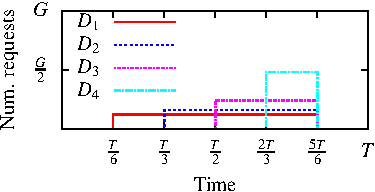
\includegraphics[width=2.25in]{figures/cate/dummy4-crop.pdf}
        \caption{$N=4$}\label{fig:1b}
    \end{subfigure}
    \caption[Number of requests to cross traffic servers.]{Number of requests from $C$ to cross traffic servers $D_i$ for different values of $N$}
    \label{fig:demand}
\end{figure}

The settings used for all simulations, including those previously shown in figure \ref{fig:two}, are as follows.
Total simulation time $T$ is set to $1200$ seconds, while total bandwidth $B$ is fixed at $240$Mbps. 
The number of requests $G$ sent from $C$ to $S$ is set to 240. 
Upon completing, a request is respawned after an idle period following an exponential distribution with a $15$s mean. 
Transfer size follows a Weibull distribution with an average value of $2$MB. 
While artificial, these values attempt to represent traffic to a single prefix with a file size that mimics the small but bursty nature of web traffic, which does not lend itself to being balanced by the end-host. 
\ac{PREFLEX} is configured with $\beta_E = 0.05$, $\mu_{min}=0.01/N$ and $\delta=0.005$.

\subsection{Varying bottleneck distribution}

For the remainder of this section, congestion balancing using \ac{PREFLEX} will be directly compared to equalisation, which mimics existing traffic engineering techniques based on hashing flow tuples for path assignment.
A useful reference point in interpreting results is to examine the case where all bottlenecks share the same bandwidth, $L_i=B/N$.
Under such conditions, figure \ref{fig:goodputeq} shows the goodput, calculated as the total data transfered to client $C$ by flows completed within $T$, as a proportion of total link bandwidth.
The bulk of goodput originates from server $S$, which is the only multi-homed domain.
If traffic is correctly balanced, servers $D_{1-N}$ should generate the same amount of goodput.
While both equalisation and congestion balancing saturate most available bandwidth, the former leads to disproportionate distribution of goodput amongst competing traffic. 
As loss is not equalised over all paths, the amount of goodput achieved by servers $D_i$ differs despite demand being similar.
\begin{figure}
    \centering
    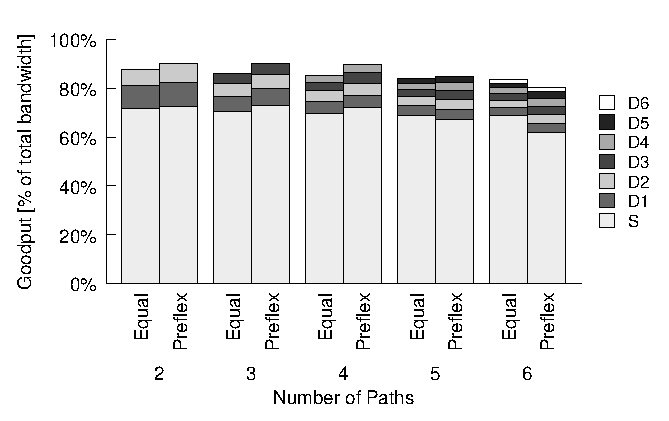
\includegraphics[width=4in]{figures/cate/eqbw}
    \caption[Goodput achieved over equal capacity links.]{Goodput relative to $B$ achieved by each server over equal capacity links.}
    \label{fig:goodputeq}
\end{figure}

In this scenario, equalisation can be seen as the optimal static TE solution, yet both approaches bear similar performance. 
With no knowledge of topology, link bandwidth or expected traffic matrices, \ac{PREFLEX} is able to adequately mimic the performance of the static TE solution for the case where such an approach is best suited.

\begin{figure}
    \centering
    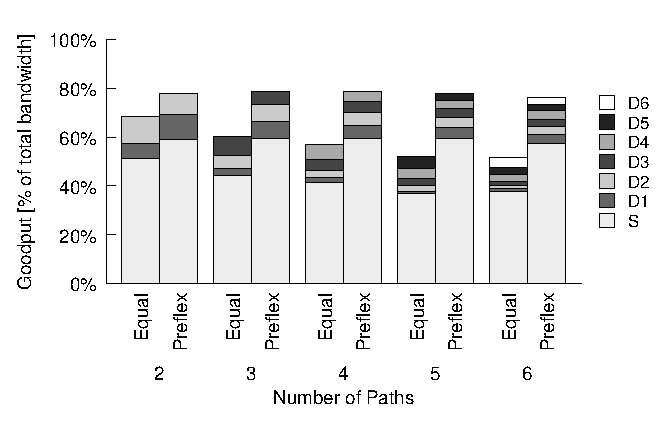
\includegraphics[width=4in]{figures/cate/diffbw}
    \caption[Goodput achieved over unequal capacity links.]{Goodput relative to $B$ achieved by each server over unequal capacity links.}
    \label{fig:goodputdiff}
\end{figure}

Where bottleneck bandwidth is unequal however equalisation is shown to be severely lacking.
The effect of differing bottlenecks is investigated by repeating previous simulations with the same total bandwidth $B$, but with $L_i$ set proportionally to $B$ in a similar manner to \eqref{eq:gi}, that is $L_i = \theta_i B$.
The ensuing results, shown in figure \ref{fig:goodputdiff}, highlight two significant shortcomings of equalisation which \ac{PREFLEX} overcomes. 
Firstly, goodput for $S$ drops as $N$ increases. 
Unable to realize it is overloading a path, equalisation is reduced to sending traffic over each link at approximately the same rate as the most congested link. 
In contrast, \ac{PREFLEX} detects congestion and adapts accordingly. 
Secondly, the incorrect distribution of traffic due to equalisation in $S$ distorts the goodput of competing traffic. 
While in \ac{PREFLEX} goodput from $D_{1-N}$ is perfectly balanced, with equalisation traffic crossing the most congested links are directly affected by another domain's inability to distribute traffic appropriately.
It may seem unfair to judge equalisation for cases where there is a mismatch in link capacity.
However, such a mismatch between link weight and path capacity arises regularly as operators adjust traffic engineering according to local conditions, with little thought spared for the impact this may have further downstream.

\begin{figure}
    \centering
    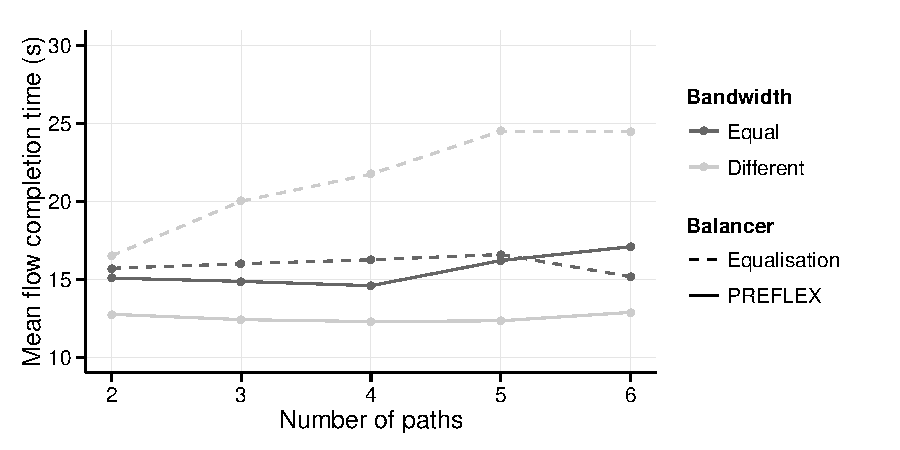
\includegraphics[width=3.2in]{figures/cate/duration}
    \caption[Mean flow completion time.]{Mean flow completion time for equal and differing bottleneck links.}
    \label{fig:duration}
\end{figure}

This impact is in turn perceived by users, who experience longer flow completion times, as shown in figure \ref{fig:duration}. 
In the equal bandwidth case the flow completion time is similar for both balancers.  
Where bandwidth differs however, balancing by congestion outperforms equalisation and maintains a stable performance even for all six paths.  
This shows that the algorithm scales well as the number of available paths increases. 

\section{Closing the loop}

This chapter broadly describes an architecture which shares the responsibility for resource pooling between end-hosts and edge networks, but does not explicitly dictate an outcome. \ac{PREFLEX} has been designed to take into account the inevitable tussle which will occur between both, and envisages use cases where control over resource pooling could feasibly shift entirely in one direction or the other. 

At its most liberal, \ac{PREFLEX} enables resource pooling to be entirely performed by end-hosts. At its most conservative, \ac{PREFLEX} affords edge network providers more fine-grained control over traffic than before. Between either extreme, the resulting mutualistic architecture offers greater transparency, control and robustness by realigning the interface between network and transport in order to accommodate the needs of both.

In order to make \ac{PREFLEX} deployable, the scope of the architecture has been restricted to stub domains.
While this necessarily reduces the amount of path diversity which can be explored, there are compelling reasons to abdicate some flexibility in favour of a more practical solution:

\begin{itemize}
\item{
    \textbf{Most benefit derives from a limited set of paths}.
    Work on source routing \cite{Gummadi:2004p131,Yang:2006p405} suggests most improvement in resilience can be extracted from a small set of deflections.
    Stub domains such as \acp{ISP} and enterprise networks are naturally multi-homed, and can provide reasonable path diversity given an adequate selection of providers.
    Expecting the establishment of cross-domain paths has been a pitfall for previous research in \ac{QoS} in particular and is marred by difficulties in providing incentives for all parties involved.
}
\item{
    \textbf{Stub domains are most aligned with user interests}. 
    For enterprise, academic and content distribution networks, end-hosts are typically managed by the same entity which operates the network.
    For \acp{ISP}, there is a binding contract between end-users and provider.
    In either case, the stub domain not only benefits from not deteriorating the quality of service provided to hosts locally, but also has an interest in making sure end-to-end traffic is unaffected by outages or degraded performance.
    The inability to reach a website is often misdiagnosed by users as a failure of the stub domain, rather than the intervening network path or the remote host.
    As a result, the burden of remote failures is often placed on local customer support.
    \ac{PREFLEX} allows resources not only to be shared more efficiently, but also potentially reduces the impact of remote network events on stub domains.
}

\item{
    \textbf{The Internet topology is flattening}. 
    In studying over 100 \acp{ISP}, transit providers and content providers for over two years, Labovitz \emph{et al.} \cite{Labovitz:2010p175} established the changing nature of the Internet topology, migrating from a hierarchy of providers to an increasingly interconnected model.
    The rise of \acp{IXP} where customer networks peer directly with content providers has had a profound impact in shaping traffic patterns and interdomain traffic in particular.
    The length of \ac{AS} paths has decreased for most \emph{content}.
    As a consequence, it has become simpler for a stub domain to ensure path disjointness as a larger portion of the end-to-end path is under its control.
}
\end{itemize}

The resulting architecture provides many benefits. 
Balancing is both transport agnostic and allows flow state to be kept to a minimum, requiring policing at the edges only if congestion accountability is required. 
Additionally, path selection is receiver driven, aligning the stakeholder who can decide when to issue \ac{FNE} packets with the stakeholder who benefits the most. 
The key to path selection is the information provided by the sender (point 7 in figure \ref{fig:preflexout} ), which allows the network to estimate path loss on the same timescale as hosts. 
By pooling loss information from multiple hosts, the network may additionally be made aware of path failures sooner than hosts using \ac{TCP} inference.

%We assume for the entirety of this section that each flow follows a single path and that a host does not override the path selected by its network, although neither is strictly necessary. 
%The implications of both assumptions being broken and the incentives involved are briefly reviewed in \cite{Araujo:2010p224}.


\chapter{A longitudinal analysis of \acs{TCP} traffic}
\label{chapter:malawi}

\renewcommand{\locfolder}{\chapfolder/malawi}
While the Internet has become evermore interconnected, exploring path diversity has been relegated to an afterthought in an architecture modeled around assumptions that no longer stand. 
Single-path forwarding as a paradigm arose not as a guiding principle, but as a natural aversion towards increasing both the complexity and cost of a resource starved network.
%engineering for scarcity worked, but cracking
Engineering for scarcity has propelled the Internet to an unprecedented scale, but problems arise when what was otherwise scarce becomes plentiful. 
Protocols designed to be bit conservative at the expense of latency have become technological anachronisms as bandwidth costs continue to plummet. 
Similarly, the notion of a router as a device merely capable of forwarding packets has long been obsolete as Moore's law continues to pave the way for greater functionality within the network. 
\ac{NAT}, \ac{DPI} or \ac{PEP} are all examples that when it comes to drawing a boundary between network and transport, the line begins to blur \cite{Ford:2008p34}.

%% paralelism increasing
Furthermore, parallelism seems to be a dominant trend at every level of the Internet architecture as a cost-effective means of increasing both performance and robustness. 
At the inter-domain level, the \ac{AS} graph is becoming flatter and more highly interconnected \cite{Haddadi:2010p129}. 
Within domains, the sheer complexity of managing paths has led to the streamlined design and deployment of \ac{MPLS} \cite{Rosen:2001p147}, implementing a fully fledged layer in its own right. 
At the edges the rise in multi-homing continues to increase the strain on an already overloaded routing architecture. 
Even within network components, parallelism is such that packet re-ordering can no longer be considered pathological \cite{Bennett:1999p120}.

Given these trends, one would expect the ability to pool traffic across such emergent path diversity to have become a network primitive. 
In reality, each stakeholder in the Internet architecture seems to balance traffic according to their needs while attempting to remain inconspicuous to others. 
At best, this interaction between stakeholders can be seen as a form of commensalism, where one entity can extract benefits while others remain unaffected. 
At worse, the competitive nature of the tussle \cite{Clark:2005p67} that ensues can spiral into a situation where few profit.

This chapter investigates the nature of this antagonism between network and endpoints and reflects on how the Internet can accommodate the needs of both through the use of \ac{PREFLEX}, a proposed architecture for balancing congestion which foments mutualism between end-hosts and edge network providers.

\section{Related work}
\label{section:malawi:related}

Despite their inherent value, longitudinal studies of Internet phenomena are rare. 
Over its short lifespan the Internet has been shaped as much by technological change as by political and commercial realities. 
This dynamic nature does not lend itself to observational studies where data must be collected and curated over long periods of time, and has resulted in a scarcity of relevant datasets. 
What few exceptions exist often stem from collaborative research efforts, such as CAIDA \cite{CAIDA} or Oregon Routeviews \cite{routeviews}. 
The usefulness of these datasets however can be severely affected by the need for data privacy. 
The dissemination of interdomain routing information, where no such requirement exists, has assisted in a wealth of research on wide ranging topics, from quantifying path diversity \cite{Oliveira:2009p203} to locating Internet bottlenecks \cite{Hu:2004p96}. 
In contrast, longitudinal datasets relating to passive measurements have nurtured a much smaller community of researchers often focusing on characterizing traffic \cite{Fontugne:2010p413}. 
Stripped of the locality contained within IP addresses however, researchers are left unable to relate these findings to a wider context.
Instead, cross-sectional studies characterizing traffic aggregated by location are frequently conducted under different contexts \cite{Ager:2011:WCC:2068816.2068870}, but lack the temporal perspective only longitudinal studies can afford. 
Efforts to characterize the spatial properties of traffic over time \cite{Dhamdhere:2011p428,Labovitz:2010:IIT:2043164.1851194,Cho:2008:OSC:1544012.1544024} have defined the changing of Internet topology and traffic alike but fall short of relating such shifts with their impact on relevant metrics such as loss or delay. 

% other work since
This chapter builds on a wealth of prior work on understanding Internet traffic and serves as a reappraisal of significant past contributions.
Flow characteristics and \ac{TCP} behaviour at large are subject to frequent reassessment \cite{Zhang:2002p85}.
Of particular relevance to the current work are passive studies which delve into the inner mechanisms of \ac{TCP}.
In \cite{Jaiswal:2004p242}, Jaiswal et al.\ infer the sender's congestion window by identifying the congestion control variant from the behaviour observed during loss recovery.
The use of separate state machines for each variant however proves unscalable given the many flavours of \ac{TCP} congestion control which have since been deployed.
In \cite{Lan:2006p566}, Lan et al.\ analyse flows according to size, duration, rate and burstiness and characterise the observed correlations for heavy-hitters specifically,
uncovering evidence of increased application influence on flow rates and burstiness and consequently suggest treating flow size and duration as independent dimensions.

One central aspect to the analysis of \ac{TCP} behaviour is the estimation of \ac{RTT} from packet capture data. 
In addition to SYN-based methods, Shakkotai et al.\ \cite{Shakkottai:2004p408} evaluate further techniques to estimate the \ac{RTT} of a unidirectional flow. 
The \textit{rate change} method establishes a relation between the \ac{RTT} and the increase in sending rate, assuming linear window increases during congestion avoidance. 
Unfortunately, this assumption no longer holds, both due to the proliferation of less conservative congestion control algorithms such as CUBIC \cite{Ha:2008p471}, and due to application-driven flow control. 
An alternative is the use of frequency-domain techniques \cite{Veal:2005p412,Lance:2005p565,Qian:2009p429}, which are a natural fit given the self-clocking nature of \ac{TCP}. 
However, a common difficulty with the application of spectral analysis is extracting the fundamental frequency which corresponds to the \ac{RTT} in the presence of noise. 
In applying the Fourier transform to inter-packet arrival times, for example, Qian et al.\ \cite{Qian:2009p429} note that less than half of all flows have distinguishable \textit{flow clocks}; likewise, the \ac{FFT}-based \ac{RTT} recovery was found to be unreliable even after pre-processing available data to enhance inherent periodicities.

% topological influence
Finally, it is important to elucidate what changes in traffic properties are intrinsic to \ac{TCP} and data transfer, and which ones arise from large-scale changes in the \ac{AS}-level topology of the Internet. 
In the decade since publication of \cite{Zhang:2002p85}, the Internet has undergone significant changes, shifting from a broadly hierarchical form to a flatter, more interconnected structure \cite{Labovitz:2010p175,Ager:2012p567}.
Given the longitudinal nature of this chapter and its focus on interdomain traffic in particular, the insights provided by these studies on the macroscopic effects of content consolidation are discernible within the studied dataset, and as such are a source of validation for many of the observations herein.

\section{Dataset}
\label{section:malawi:dataset}

This section provides an overview of the datasets used in this work and some of the data processing required before approaching the longitudinal study of Internet traffic rate limiting. 
The dataset used is composed from the original, un-anonymised traffic traces from the \ac{MAWI} dataset \cite{mawi}, a set of daily packet captures from the \acs{WIDE} backbone network which provides connectivity to universities and research institutes in Japan. 
Traffic is collected daily for 15 minutes starting at 14:00 \acs{JST}. 
Although this dataset extends back largely uninterrupted from late 2001, the present work focuses on just over five years of data following a network upgrade to the monitored link on October 2006.
The monitored link carries mostly trans-Pacific commodity traffic between \acs{WIDE} customers and non-Japanese commercial networks. 
Traffic towards \acs{WIDE} is referred to as \emph{inbound} traffic, whereas traffic originating from within \acs{WIDE} is referred to as \emph{outbound} traffic.

\begin{table}[!htp]
\footnotesize
\centering
\ra{1.2}
    \begin{tabular}{
@{}$ % cut edge, start row
>{\raggedright\arraybackslash}p{1.0cm} % year
^>{\raggedleft\arraybackslash}p{1.0cm}@{\hskip 1.0cm} % days
^>{\raggedleft\arraybackslash}p{1.7cm}@{\hskip 1.3cm} % flows
^>{\raggedleft\arraybackslash}p{1.0cm}                % traffic in
^>{\raggedleft\arraybackslash}p{1.0cm}@{\hskip 1.0cm} % traffic out
^>{\raggedleft\arraybackslash}p{1.0cm}                % AS 
^>{\raggedleft\arraybackslash}p{1.0cm}                % AS 
@{} % cut edge
}
\toprule
\rowstyle{\bfseries\scshape}
\multirow{2}{*}{ \parbox[][0.8cm][b]{0.5cm}{Year}} &
\multirow{2}{*}{ \parbox[][0.8cm][b]{0.5cm}{Days}} &
\multirow{2}{*}{ \parbox[][0.8cm][b]{2.5cm}{\centering TCP data \\ flows ($\times10^3$)}} &
\multicolumn{2}{c}{ \bfseries\scshape Traffic (TB) \hspace*{0.8cm} } & 
\multicolumn{2}{c}{ \bfseries\scshape Unique ($\times10^3$) } \\

\cmidrule(r{1.0cm}){4-5} \cmidrule{6-7}
\addlinespace[-0.6em] \rowstyle{\scshape\scriptsize}
& & & \centering In & \centering Out & \centering AS & Prefixes \\
\midrule

    2006 & 91 & 20.52 & 0.43& 0.45 & 10.90 & 56.86\\
2007 & 350 & 102.56 & 2.11 & 2.49& 17.21 & 113.79\\
2008 & 358 & 112.26& 2.43 & 2.10& 24.74 & 156.54\\
2009 & 364 & 113.97& 2.48 & 2.53& 19.71 & 143.87\\
2010 & 365 & 113.70& 2.58 & 3.43& 20.38 & 148.03\\
2011 & 358 & 114.74& 3.44 & 5.14& 19.99 & 140.56\\
\addlinespace[0.4em] \rowstyle{\bfseries}
Total & 1886 & 5777.55 & 13.50 & 16.14 & 34.12 & 341.22\\

    \bottomrule
    \end{tabular}
    \caption{\label{table:overview}Overview of traced \acs{MAWI} dataset.}
\end{table}

A preliminary overview of the dataset used is provided in table \ref{table:overview}. 
In total, 5.7 billion flows containing data are traced over five largely uninterrupted years; this represents approximately 30 terabytes of \ac{TCP} traffic. For the purposes of this work, most analysis will focus on inbound traffic, 60\% to 80\% of which originates from port 80, referring only to analysis of outbound traffic when contextualizing findings.
Given the sender side plays a critical role in shaping traffic, analysing traffic for which the source is restricted to a small set of networks within Japan is of limited use in accurately depicting traffic trends at large.
Hosts within Japan are instead fixed as traffic sinks, thus sharing a similar perspective on inbound traffic as many other similarly sized networks. 

\subsection{Tracing \acs{TCP} Metrics}

All \ac{TCP} flows are reassembled and analysed for each daily trace.
In addition to the five tuple used to define each connection, two additional restrictions are imposed: a contiguous sequence number space and a three minute timeout. 
These restrictions are helpful to deal with port reuse and unterminated flows respectively.  
Although the total number of \ac{TCP} flows increased dramatically in 2011, the number of flows for which data payload was observed has remained stable, averaging over 100 million data flows traced per year.  

There is much prior work with regards to reconstructing \ac{TCP} flow from passive measurements and using this information to understand the end-to-end properties of traffic \cite{firstRTT,Jaiswal:2007p233,Rewaskar:2007p195,Shakkottai:2004p408}. 
However, the \acs{MAWI} traces impose two constraints which require careful consideration, and ultimately led to the use of a custom \ac{TCP} tracer. 
The first is the proportion of bidirectional flows, where both forward and reverse path are seen. 
In the dataset used this fluctuates between 40\% and 60\% over five years.
Most available \ac{TCP} tracers either ignore or are inadequate at processing unidirectional flows. 
The second is the short duration of each individual trace file. 
At only 15 minutes of line-rate data capture per day, it is wasteful to ignore flows which are not complete. 
Although the number of flows for which a SYN and FIN in either direction is observed has remained consistently high until late 2011, these flows are normally \emph{mice}, i.e. flows that tend to be brief and which carry little traffic individually. 
In contrast, most \emph{elephants} (flows that carry significant traffic individually) have durations that exceed that of each trace file. 

Loss is inferred by accounting for \emph{retransmissions} in the upstream data and \emph{out-of-order packets} in downstream data; for the remainder of the paper the term \emph{end-to-end loss} will refer to the sum of out-of-order and retransmitted data bytes over the total data bytes in a given direction.
Anecdotally, this was found to be an adequate indicator of loss --- with the exception of \emph{hanging} \ac{TCP} connections. 
In such cases where connectivity is lost, a host will proceed to retransmit packets while performing an exponential back-off. 
Although this results in negligible overall traffic, it can significantly skew the inferred loss ratio for uncommon destinations for which little traffic exists. 
To account for these cases, a 3-second timeout on retransmissions was imposed, after which the congestion feedback loop is considered to be broken. 

Each daily trace in the dataset is processed from a packet level capture into a collection of flow level statistics, providing insight into the end-to-end characteristics of traffic. 
However, since a core objective of this work is to augment this time-based information with data describing the endpoints of each flow, aggregating by location is also required. 

\subsection{Aggregating by Location}

Location information is added by mapping the original source and destination \ac{IP} addresses to its geographical and topological counterpoints. 
The routeviews archives \cite{routeviews} are used to reconstruct the mapping between each \ac{IP} and both \ac{AS} and network prefix; bi-hourly dumps of \ac{BGP} \acp{RIB} are available in the \acs{WIDE} archives since mid 2003. 
A daily \ac{RIB} is reconstructed based on the views provided by contributing \acp{AS}, in particular \acs{IIJ} and \acs{APNIC}.
Since there is no record of local policy, exact routes are not disclosed and as such there is no prior knowledge of the route taken by packets; this however does not hinder the ability to consistently map \acp{IP} to \acp{AS}.
While discrepancies in \ac{AS} destinations exist between different routeviews contributors, this happens almost exclusively on prefixes for which no actual traffic is seen. 

Mapping \ac{IP} to country is done through the use of GeoLite \cite{maxmind}, a commercial geolocation database. 
While the accuracy of this solution is often disputed, locating traffic at a fine granularity is not a pressing concern.
Most geographic emphasis will be placed on capturing macroscopic shifts in time at a national level, for which Geolite proves adequate.
The archive for geolocation data only extends to 2009, before which the earliest match must be used.
Additionally, the administrative mapping up until mid 2009 for a destination or source \ac{AS} is verified to have remained the same in the relevant \ac{RIR} archives in order for a flow to be assigned a geographical location.
% bridging paragraphs to save space.
After associating flows to country, region, \ac{AS} and network prefix for both source and destination \acp{IP}, flow statistics are aggregated over each location identifier. 
This generates a daily collection of location identifiers and associated flow properties, from which the geographic and topological properties of the dataset can be sketched over time.

\section{Methodology}
\label{section:malawi:methodology}

Providing a macroscopic view on where traffic originates from, and in what quantity, can be achieved by simply binning packets into flows and accumulating byte counts over geographical or topological locations. 
Uncovering application layer characteristics (i.e. \textit{how} traffic is sent) is a more complex problem that requires additional methods to reverse engineer transport behaviour.
The aim of this section is to describe a process which distinguishes those flows which have their throughput limited by mechanisms other than the usual \ac{TCP} response to loss and delay.
Each flow can be characterized as being either application paced, in which the sending application is limiting the data provided, host limited, whereby local constraints at either end host cap throughput, or receiver shaped, in which an artificial constraint is imposed by either a middlebox or receiver.

The classification proceeds in stages. 
Before classification, if a flow is not bidirectional its RTT must be recovered.
This is achieved in section \ref{subsection:malawi:PeriodicEnhancement}. 
Because the sender's TCP state machine cannot be directly observed, the congestion window must be instead estimated by observing the number of unacknowledged bytes in flight (\textit{flight size}).
This reconstruction is described in section \ref{subsection:malawi:flightAggregation} and provides the basis for flow classification. 
Flows are then checked in turn to see if they are application paced, host limited or receiver shaped and classified as belonging to the first of these classes for which they fulfill the necessary conditions.
Flows in none of these classes are either limited only by the network (delay or loss conditions) or are insufficiently large for constraints to be reliably detected.

\subsection{\acs{RTT} Estimation}
\label{subsection:malawi:PeriodicEnhancement}

Building on prior work presented in section \ref{section:malawi:related}, this section proposes an algorithm that scalably recovers the RTT from one-directional traffic traces. 
% XXX: below implies microflights were used, but these aren't described (remove as appropriate)
Although \ac{RTT} estimation is a difficult problem, simplifying assumptions can be made.
For the \acs{MAWI} dataset most \acp{RTT} are relatively large, with the closest neighbouring country, South Korea, roughly 40ms away.
By only processing bidirectional traffic from Japan, the expected \ac{RTT} range can be reduced for all other traffic.
The recovery mechanism then enhances the natural periodicity of traces and scalably constructs flights associated with specific application and protocol behaviour.
In the following the mechanisms required by these two goals are described. 
%
% Why does this work?
%
In normal operation, many \ac{TCP} operations involve request-response cycles between two endpoints in which the \ac{RTT} $T$ provides a natural \emph{clock}.
Hence, the most natural way to estimate \ac{RTT} from \ac{TCP} traces is to correlate requests and responses exchanged in both directions. 
If only one direction of data is observed however, $T$ cannot be directly observed. 
Instead, it must be estimated from the way in which \ac{TCP} packets cluster in time due to the batching of request-response operations.

The \ac{TCP} \ac{cwnd} determines the number of unacknowledged bytes that a \ac{TCP} flow may maintain at any point in time. 
This can be referred to as \emph{bytes in flight} because they are in transit between the sender $S$ and the receiver $R$; an equivalent definition applies for the number of \emph{packets in flight}. 
Once $S$ has transmitted \ac{cwnd} data bytes, it will refrain from transmitting more until either some bytes are acknowledged by $R$ or \ac{cwnd} is increased by the sender. 
In the absence of losses, neither of these events can happen until a \ac{TCP} \ac{ACK} is received; this immediately reduces the number of unacknowledged bytes, but may also lead to a significant \ac{cwnd} increase (during e.g. \emph{slow start}). 
% XXX: number of unacknowledged bytes reduced, or CWND?
In the presence of losses, however, bytes can be re-sent if a packet is timed out and considered lost; in this case, the number of unacknowledged bytes is reduced.

%
% What is our main contribution, algorithmically speaking?
%
The main difficulty associated with one-sided TCP flow reconstruction is as follows.
Let $t_1, t_2, \ldots$ be a set of times at which packets $p_1, p_2, \ldots$ were observed at $S$ en route to $R$.
Suppose that a packet $p_j$ of size $b$ is observed at time $t_j$.
In addition, suppose that approximately one RTT $T$ later, the sender $S$ receives an ACK $a_j$ from $R$ for the $b$ bytes of $p_j$.
At this point, the TCP stack in $S$ will decrease the number of unacknowledged bytes by $b$, thus opening the possibility for sending additional traffic to $R$.
This can lead to another packet $p_k$ to be transmitted; let this packet be observed at time $t_k$ as it is sent towards $R$.
Assuming that processing delay is insignificant, the RTT experienced by $p_j$ can be approximated as $T \approx t_k - t_j$.
Now consider what happens if packets are only observed in the $S \rightarrow R$ direction.
Under such conditions, it is not possible to ascertain whether $p_k$ was sent explicitly as a result of $S$ receiving the unobserved \ac{ACK} $a_j$, or whether it was sent as a result of an \ac{ACK} $a_i$ associated with a previous packet $p_i$ rather than with $p_j$.
If, however, a packet $p_l$ is eventually observed that did result from the reception of $a_j$, the \ac{RTT} can be estimated as $T \approx t_l - t_j$ with $t_l > t_k$.
Following this same reasoning, approximately one \ac{RTT} later a packet $p_m$ will be observed for which $2T \approx t_m - t_j$; this can potentially continue for as long $S$ has data to send and $R$ continues sending \acp{ACK}.
This is the underlying reason that \ac{RTT}-related periodic regularities arise when considering the timestamps of observed packets \cite{Qian:2009p429}.

The reasoning above is at the heart of the proposed algorithm to improve \ac{RTT} recovery by enhancing packet stream periodicity. 
Assume that a packet $p_j$ is observed at time $t_j$. 
Considering the set $\mathcal{T}_j$ of all values of $\Delta t = t_k - t_j$ for every $k > j$, it is apparent that it will include estimates not only for the \ac{RTT} $T$, but also for all its multiples $2T, 3T, \ldots$ 
If $t_l-t_k \approx T$ and $t_k - t_j \approx T$ then it follows that $t_l - t_j = 2T$, and this value will also be included in $\mathcal{T}_j$. 

By maintaining a set $\mathcal{T}_j$ for every packet $p_j$ observed, at least some of its values will correspond to estimations of multiples of the \ac{RTT}. 
It then follows that by creating a set $\mathcal{T}$ that includes values calculated starting from every packet $p_j$ so that $\mathcal{T} = \cup_j \mathcal{T}_j$, numerous estimates for $2T, 3T, \ldots$ will also be included. 
Hence, the probability density function $H(t)$ of the values in $\mathcal{T}$ should show peaks around multiples of the \ac{RTT} (see Figure \ref{fig:histogram}). 

\begin{figure}
  \centering
  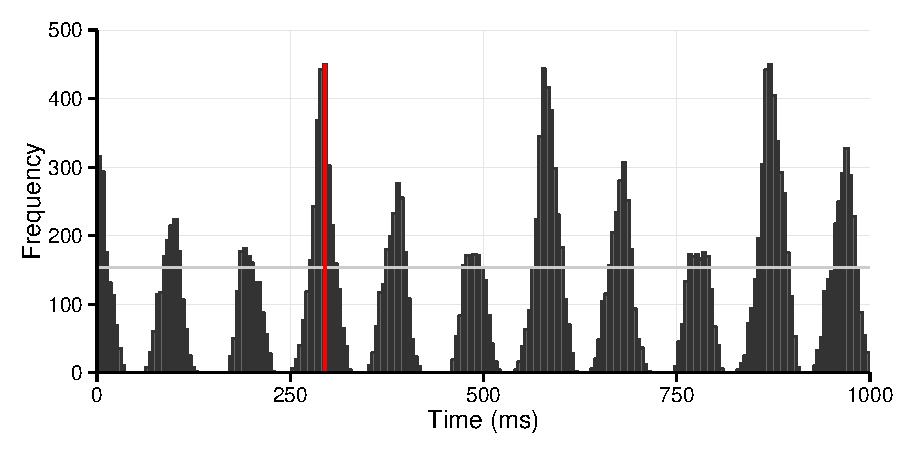
\includegraphics[width=0.8\textwidth]{figures/malawi/rttbin.pdf}
  \caption{$H(t)$ for flow displayed in Figure \ref{fig:hostlimited}. The horizontal line delimits $\overline{H}$ while the highlighted bin denotes the bidirectional RTT estimate.\label{fig:histogram}}
\end{figure}

%
% Explain why did we use FFT
%
The algorithmic recovery of $T$ from $H(t)$ presents additional challenges. 
In particular, $H(t)$ may include a large number of \ac{RTT} multiples, and a peak will be found for all of them. 
Crucially, all these peaks may be of comparable magnitude, complicating the task of selecting a single peak.
Moreover, these peaks need not be very pronounced, with histogram bins in close proximity of the peaks have very similar values as the peak itself. 
As such, taking \ac{RTT} candidates directly from $H(t)$ may result in a large set of similarly-valued bins situated around a peaks at multiples of the \ac{RTT}. 

Three recovery algorithms for $T$ are attempted.
First, as a baseline, the highest peak in $H(t)$ is selected as a candidate for $T$. 
In addition, expanding upon the work of Qian et. al. \cite{Qian:2009p429} a frequency-domain representation of $H(t)$ is used to identify $T$. 
This is done by selecting the highest peak of $|\hat{H}(\omega)|^2$, the \emph{energy spectral density} of $H(t)$ (i.e. the norm squared of the Fourier transform of $H(t)$). 
Finally, a custom utility-based technique that operates directly on $H(t)$ is proposed which achieves superior performance to both of the aforementioned methods.

%\subsubsection{FFT-Based RTT Recovery}
%We extract periodicity information from $H(t)$ by looking at $\hat{H}(\omega)$, the \emph{energy spectral density} of $H(t)$. Formally, $\hat{H}(\omega)$ is defined as the norm squared of the Fourier transform of $H(t)$, so that $\hat{H}(\omega) = |\mathcal{F}(H(t))|^2$. Using $\hat{H}(\omega)$ markedly improves the quality of our RTT estimation because the frequency peak corresponding to the RTT usually accounts for a much larger proportion of the total frequency domain energy than other peaks in $\hat{H}(\omega)$, leading to a much simpler discrimination of the true RTT. However, due to RTT changing during the lifetime of a flow, and also due to the expected noise associated with real-life data sources, $\hat{H}(\omega)$ can also occasionally include large peaks at frequencies unrelated to the RTT. In order to filter these out, we take a set of 10 frequency candidates from $\hat{H}(\omega)$, and use their associated periods as RTT candidates in our flow reconstruction algorithm (see Section \ref{
%subsection:malawi:flightAggregation}). We then select that RTT candidate which exhibits the smallest error, that is, that one which yields closest agreement with observed data.

%
% Algorithmic hacks
%
%To streamline our algorithm for streaming use, we use the following heuristics and approximations. Firstly, we define a range $[T_{\min}, T_{\max}]$ representing the range over which we find the RTT values of interest. Then, for each packet $p_j$, we build a subset $\mathcal{T}_j'$ of $\mathcal{T}_j$ by including all values of $t_j - t_k < T_{\max}$. We then generate $\mathcal{T}' = \cup_j \mathcal{T}_j'$ and approximate $H(t)$ by considering a histogram of the values in $\mathcal{T}'$. As usual, we do this by counting the frequency with which its values are observed in the ranges $[0,\tau)$, $[\tau, 2\tau)$, $[2\tau, 3\tau), \ldots$ where $\tau$ is the time resolution required. 


\subsubsection{Utility-Based RTT Recovery}
\label{sect:utilityBasedRecovery}

This method relies not on the identification of periodicities, but on explicitly matching experimentally found signatures. 
To this end, we consider the peaks of $H(t)$, which are then considered RTT candidates.  
However, trivial discriminators (such as simply selecting the highest peak) are not reliable. 
In this case, it was found experimentally that repeatable peaks and troughs also occur at multiples and sub-multiples of $T$, with the most important ones being $\frac{T}{3}$, $\frac{T}{2}$, $T$ and $2T$. 
We design this detection algorithm around the idea that a given pattern of peaks and troughs can identify $T$.

If we define $\overline{H}$ as the mean height of $H(t)$, we can define a per-peak utility function $p(t)$ so that 
\begin{equation*}
p(t) = 1.0 - \exp\left(-2.0 \left(\frac{H(t)}{\overline{H}}\right)\right) \mbox{.}
\end{equation*}
This function has several advantageous properties: it is 0 if $H(t)$ is zero, 1
if $H(t)$ is infinite, and $0.5$ if $H(t) = \overline{H}$.  In other
words it is a measure of the \emph{peakiness} of the data, with $p=1$ identifying
an infinitely high peak, $p=0$ identifying an empty histogram bin (trough), and $p=\frac{1}{2}$ 
implying that $H(t)$ is of exactly average height at that point. We can then score each candidate using the following utility function:
$$
P(t) = 1.5 p(t) + p(2t) - p\left(\frac{t}{2}\right) - p\left(\frac{t}{3}\right).
$$
That is, the candidate RTT $t$ scores highly if it is itself a peak, if it has a peak
at a multiple $2t$, and if it also manifests troughs at submultiples $\frac{T}{2}$ and $\frac{T}{3}$.
The factor of 1.5 was added after observations
showed that the peak at $T$ was the most important factor in determining
whether a candidate was the true RTT. Similarly, additional multiples and submultiples 
were excluded as they showed very limited discriminating power experimentally.

\begin{figure}
  \centering
  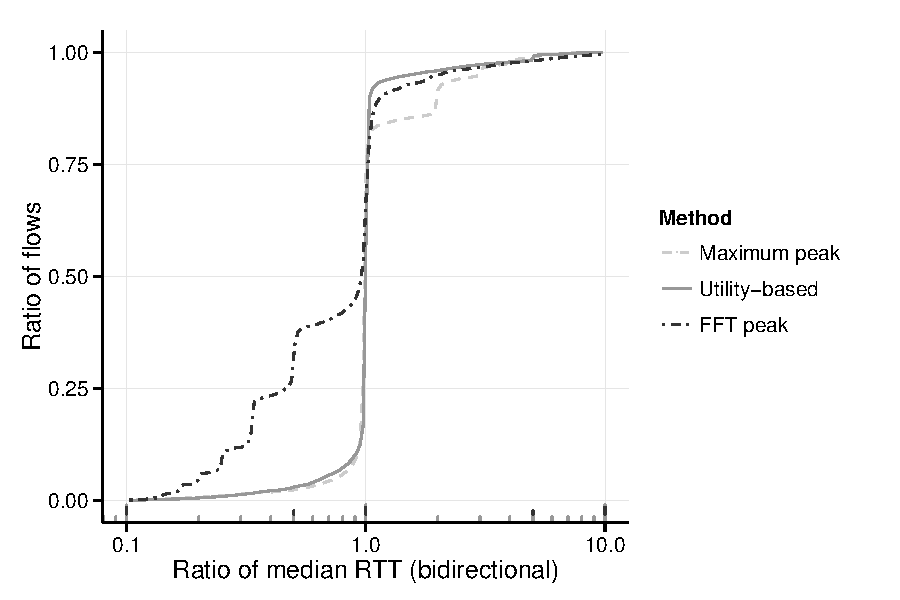
\includegraphics[width=0.8\textwidth]{figures/malawi/rttcomp.pdf}
  \caption{Accuracy of RTT estimator when compared to the median value of bidirectional estimate.}
\end{figure}

\subsubsection{Comparing RTT Recovery Algorithms}
\label{sect:comparingRecoveryAlgos}
As described in Section \ref{subsection:malawi:PeriodicEnhancement}, $H(t)$ is calculated in such a way that RTT periodicity is amplified. 
This means that FFT-based techniques could potentially perform better on $H(t)$ than on the packet stream with no pre-processing. 
However, this is complicated not only because $H(t)$ contains periodicities at multiples of $T$, but also discontinuities that generate harmonics at frequency multiples of the RTT fundamental. 
Hence, although the FFT $|\hat{H}(\omega)|$ of $H(t)$ is much cleaner than that of the packet interarrival time series on its own, its maximum peak rarely coincides exactly with the RTT clock (this corroborates reports by Qian et al \cite{Qian:2009p429}). 
Thus, applying the FFT leads to another \emph{peak detection problem} in which the RTT fundamental needs to be extricated from its harmonics and sub-harmonics. 
The trivial solution to this problem, the application of a bandpass filter around the RTT frequency, is of course unfeasible because the bandwidth and 
centring of such a filter depend on the RTT which is itself unknown.
The utility-based algorithm described in Section \ref{sect:utilityBasedRecovery} can hence be applied in either the time domain or the frequency domain; we chose to do it on the former on the interest of expediency and lower computational cost.

\newcommand{\RTTHeader}{Below & Above}
\newcommand{\SmallFlowName}{\textless 10MB}
\newcommand{\LargeFlowName}{\textgreater 10MB} 
\begin{table}
\footnotesize
\centering
\begin{tabular}{ p{1.5cm} p{1.2cm} p{0cm} p{.6cm}p{.6cm} p{0cm} p{.6cm}p{.6cm}}
& & & \multicolumn{2}{c}{Peak} & & \multicolumn{2}{c}{Utility-based} \\
\cline{4-5} \cline{7-8}
& Flow size & & \RTTHeader & & \RTTHeader \\
\cline{4-5} \cline{7-8} 
\multirow{2}{*}{Receiver side}  & \SmallFlowName && 4.31 & 9.13 && 4.58 & 6.35
\\ 
                                & \LargeFlowName && 6.72 & 6.43 & 4.97 & 5.33
\\
\multirow{2}{*}{Sender side}    & \SmallFlowName && 2.94 & 8.37 && 3.29 & 4.80
\\
                                & \LargeFlowName && 6.41 & 9.06 & 5.40 & 11.06
\\
\end{tabular}
\caption{\label{table:rttRecovery}Performance of RTT recovery algorithms}
\vspace{-3mm}
\end{table}

The performance of the analysed RTT recovery mechanisms is presented in Table \ref{table:rttRecovery}, that shows the percentage of total flows below and above the RTT range given by the bidirectional estimates.
We separate things for \emph{inbound} traffic (where we are positioned at the receiver side) and \emph{outbound} traffic (where we are positioned at the sender side). The utility-based algorithm is particularly useful to address RTT underestimation for flows over 10MB in size, which is our main objective since precisely that kind of estimation error would interfere with our ability to correctly decouple application behaviour from RTT-scale dynamics.


%For the most part, the utility based method improves on underestimation, which is our main objective since that would interfere with our flight reconstruction (i.e. generate lots of gaps).
%The exception (kind of) is traffic from the sender side, which in our training set (one week per year), had quite a lot of host limited traffic (paced out, no signal to recover).
%In this case, not a problem, since if the flow is long enough multiples of the RTT will still reveal host limitation, but will give us a smaller window..


\subsection{Flow Classification}
\label{subsection:malawi:flightAggregation}

One fundamental precondition to decouple the influence that network loss, host configuration and TCP behaviour has on the throughput experienced by a flow is the reconstruction of the congestion window behaviour of TCP flows on the basis of observed data. 
Unfortunately, the congestion window value is internal to the sender's TCP state machine and may not manifest itself in the absence of sufficient data from the application layer. 
A more easily observed quantity which serves as a reasonable proxy for the congestion window is the number of unacknowledged bytes in flight, henceforth referred to as the \textit{flight size}, which can be derived given an accurate estimate of the end-to-end delay.
The evolution of both flight size and RTT can in turn be used to ascertain to what extent throughput is regulated by limitations imposed at different layers of the networking stack.

% definitions
Given a candidate RTT, we can aggregate a stream of packets with arrival times $t_1, t_2, \ldots$ into a stream of \emph{flights}. 
Intuitively, a flight is a clustered subset of a TCP flow which exhibits its own temporal coherence; alternatively, it can be though of as a series of consecutive packets that were (roughly) generated by the sender as a response to the same protocol operation. 
A flight $f_i$ that begins
with the $j$th packet and ends with the $k$th is defined to have a \emph{total flight time} $\tau_i = t_{k+1} - t_j$. 
The algorithmic selection of initial and final packets in such a way that the resulting flights are indicative of TCP behaviour remains an open problem. 
Since we assume that the RTT provides a natural time frame for the operations of TCP, in the algorithm presented in this work, given an initial packet $\pi_j$ and an RTT estimate $T$, the $k$th (and final) packet is selected to minimise \emph{the flight time error} $e_i = |T - \tau_i|$. 
This mechanism follows closely the methodology described in \cite{Zhang:2002p85}, with the exception that we do not attempt to define flights as being both adjacent and disjoint; rather, we decompose flows into a stream of potentially overlapping flights. 
This helps the algorithm mitigate the deleterious effects of small deviations in the estimated RTT, which alters the properties of each flight. 
Furthermore, since the flight size is continuous in time, it makes little sense to restrict ourselves to a single sample per round trip time.

Having obtained flight information from each flow, we next consider what is the predominant factor that affects its throughput. 
Within the context of TCP, we classify flows as being artificially constrained by three distinct processes: \emph{application pacing}, \emph{host limited} and \emph{receiver shaping}.

\begin{figure}
\centering
  \centering
  \begin{subfigure}{1.0\linewidth}
    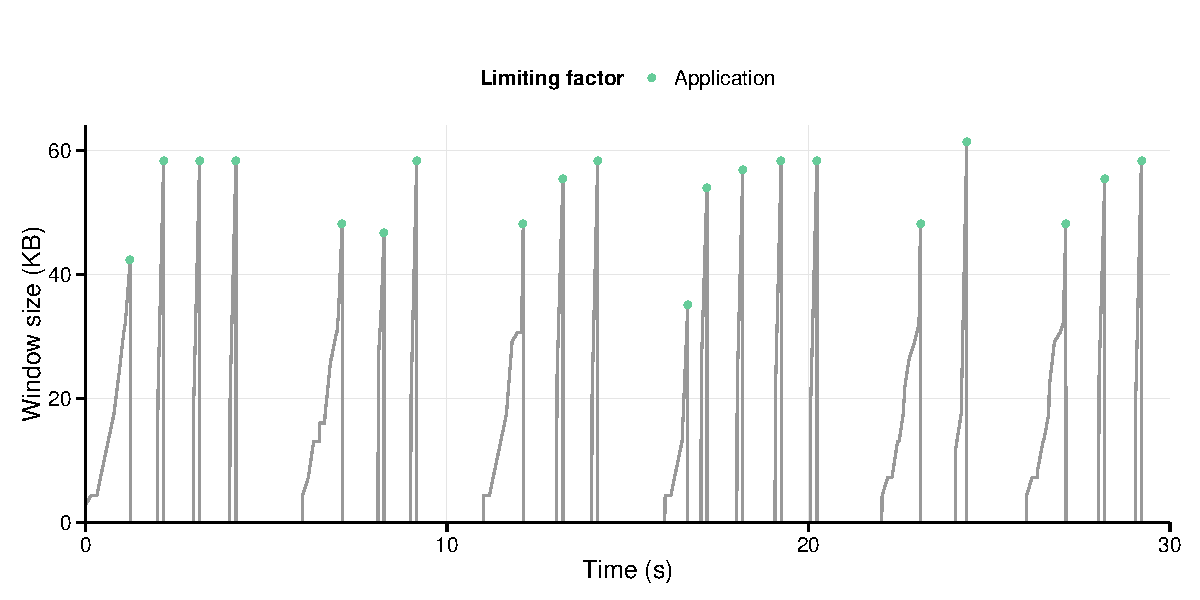
\includegraphics[width=1.0\textwidth]{figures/malawi/youtube.pdf}
    \caption{Application paced. \label{fig:youtube}}
  \end{subfigure}\\
  \begin{subfigure}{1.0\linewidth}
    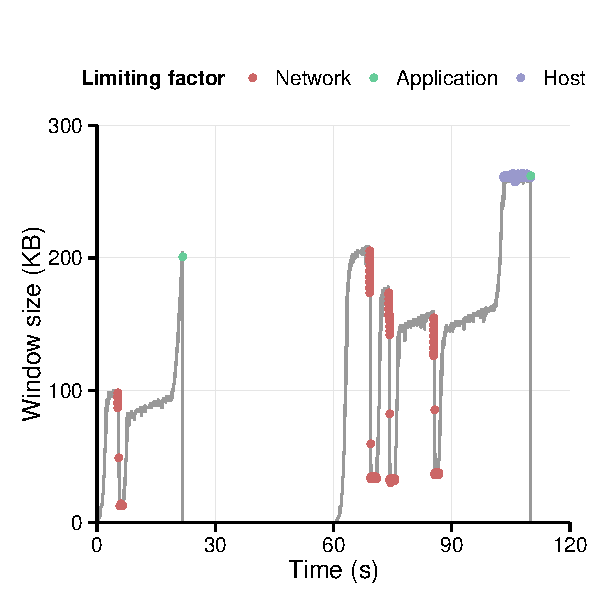
\includegraphics[width=1.0\textwidth]{figures/malawi/hostflow.pdf}
    \caption{Partially host limited. \label{fig:hostlimited}}
  \end{subfigure}\\
  \begin{subfigure}{1.0\linewidth}
    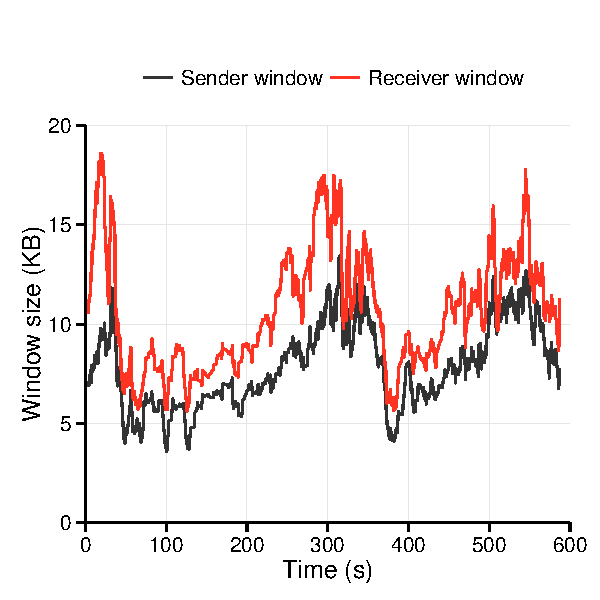
\includegraphics[width=1.0\textwidth]{figures/malawi/awnd.pdf}
    \caption{Receiver shaped. \label{fig:awnd}}
  \end{subfigure}
  \caption{Flight size over time for flows affected by different artificial constraints. \label{fig:kindsOfFlowEffect}}
\end{figure}


\subsubsection{Application Paced Flows}
\label{sssec:app}

A flow whose throughput decreases because it has no outstanding data to send is temporarily limited by the application. 
Flights can be identified as being \emph{application limited} if terminated with a packet smaller than the maximum segment size (MSS) and followed by an inter-arrival time greater than the RTT, as consistent with \cite{Zhang:2002p85}. 
The underlying reason for this defintion is that most TCP implementations will wait some time for subsequent bytes to be written to the socket if the next packet to be sent is smaller than the MSS, unless the TCP\_NODELAY option is set \cite{nagle1984rfc}.

A flow with \emph{application limited} flights however is not necessarily \emph{application paced}. In practice, all flows for which the final packet is observed contain at least one such flight.
For the purposes of our work, we are focused on identifying cases in which throughput is predominantly determined by application behaviour.
One such example is illustrated in figure \ref{fig:youtube}, in which a stream is delivered by periodically writing blocks to the sending socket.
The resulting network-level behaviour is distinct from traditional congestion control: short bursts are interspersed with protracted silence.
Application limited flights, which terminate on non-MSS packets, are highlighted at the end of each burst.

This behaviour is in stark contrast to that exhibited in figure \ref{fig:hostlimited}, where distinct transfers are multiplexed on top of a single transport association over time.
From the perspective of the network, there is little to distinguish the behaviour of such traffic from independent TCP flows.
Application paced connections such as Youtube traffic however exhibit a degree of regularity which can potentially be exploited by the network in predicting demand or smoothing bursts.

In order to identify such recurring behaviour, we identify flows as being \emph{application paced} if the period between bursts terminated by \emph{application limited flights} is consistently under 10 seconds and the standard deviation of the intermediate pauses is under one second.
This definition in particular purposely ignores flows which exhibit long silence periods due to user interaction, and follows closely the behaviour historically associated to Youtube streaming in particular.

\subsubsection{Host Limited Flows}
\label{sssec:host}

Given sufficient bandwidth and traffic to send, a flow may encounter local constraints at either end-host which cap its throughput. 
For instance, the buffer space allocated on both the sender and receiver side is often pre-configured, and it is common practice to tune these values down on popular servers and managed infrastructure in a bid to conserve memory or bandwidth.
A receiver is also limited in the window size it can announce to the remote sender; if the windowscale option \cite{jacobson1992tcp} is not negotiated during the TCP handshake, the advertised window cannot exceed 64KB.

In both cases, a local decision by either host can determine the upper bound of the flow rate.
These \emph{host limited} cases are characterised by a constant window size over time.
The methodology described for flight aggregation at the beginning of this section typically generates a large number of flights, representing many likely combinations given a base RTT estimate.
In order to identify the flat-lined behaviour of a host limited flow, we first filter the flight stream to remove some of the uncertainty derived from small fluctuations in the RTT.
We then select the maximum flight size observed for each RTT interval, and declare a sequence of flights to be host limited if the same maximum was observed over six consecutive RTTs (this is twice the period suggested in \cite{Zhang:2002p85}).
In practice, increasing the period over which the maximum window size is tracked allows us to more accurately discern between host limited behaviour and more conservative bandwidth probing, such as that performed during the convex phase of TCP CUBIC \cite{Ha:2008p471}.

A flow may be host limited for only brief periods of its lifetime, as illustrated in figure \ref{fig:hostlimited}.
To filter out such cases where host limitations are not the predominant factor in defining flow throughput, we further enforce that in addition to host-limited flights, the average window size must over a flow lifetime should be within 10\% of the inferred host limit, which is not the case in figure \ref{fig:hostlimited}.

In practice, flows can exhibit both application pacing and host limitations, with bursts being sent at a capped window size followed by application pauses.
In such cases, a flow will still be classified as being \emph{application paced} if it meets the requirements set out in the previous section, as doing so provides evidence that it controls throughput in spite of the degraded performance provided further down the stack. 
This line of reasoning applies equally to the occurrence of sporadic loss; so long as block delivery is ensured within the timeframe dictated by the application, it remains in control.

\subsubsection{Receiver Shaped Flows}
\label{sssec:rec}

A flow which is neither \emph{application paced} or \emph{host limited} can still be artificially constrained by flow control (rather than by congestion control).
Traditionally, in TCP the sender is responsible for regulating throughput. 
However, the receiver can also shape throughput by manipulating the \emph{advertised window} announced on every acknowledgement.
Such receiver-window auto-tuning has been available on Windows operating systems since Vista \cite{vistaReceiveWindow}, and can also be leveraged by middleboxes in order to throttle inbound traffic \cite{appEx}.

In order to evaluate the potential impact of such behaviour, we further propose a heuristic to identify receiver-shaped traffic.
For flows in which both directions of traffic are observed it is possible to correlate the evolution of the advertised window with the size of reconstructed flights.
Figure \ref{fig:awnd} displays an example of a receiver-shaped connection, in this case throttled by an intermediate middlebox.
Since the advertised window may be fluctuating, it is not always obvious which of the many updates were effectively applied by the sender as successive values supersede each other.
An example of a reconstructed flow which is subjected to receiver shaping is displayed in Figure \ref{fig:awnd}.

For flows in which both directions are observed, it is possible to classify flights as being receiver-shaped if there is a statistically significant correlation between the advertised window size and the maximum flight size observed.
Harnessing the stream filtering used in detecting host limited behaviour, we perform such analysis over a sliding window of 10 RTT intervals.
A flight is flagged as being receiver shaped if the correlation between receiver window and flight size is statistically significant; a flow is considered to be predominantly receiver shaped if over half of its flights are flagged as such.
We do not perform this covariance analysis on flights which contain out-of-order or retransmitted packets. 
In these cases, both the receiver and sender window sizes are correlated \emph{by definition}. 
In the former case, the receiver buffer will temporarily fill expecting the next packet in sequence, in the latter case, TCP will reduce its window.

Given that receiver shaping classification requires correlating information in both directions of a TCP connection, it will come as no surprise that the absence of the reverse path can introduce false positives into our measurements. 
This happens because any given flow might be receiver shaped in such a manner that the heuristic erroneously attributes its behaviour to host limitations. 
In the absence of additional evidence, this misclassification is difficult to detect explicitly. 
Instead, we calculate the ratio of receiver shaped flows which would have been incorrectly identified if the reverse path were not observed. 
This error rate can then be used to evaluate the accuracy of classifier results.

\section{Macroscopic traffic trends}
\label{section:malawi:macro}

\begin{figure}
  \centering
  \begin{subfigure}[b]{1.0\linewidth}
  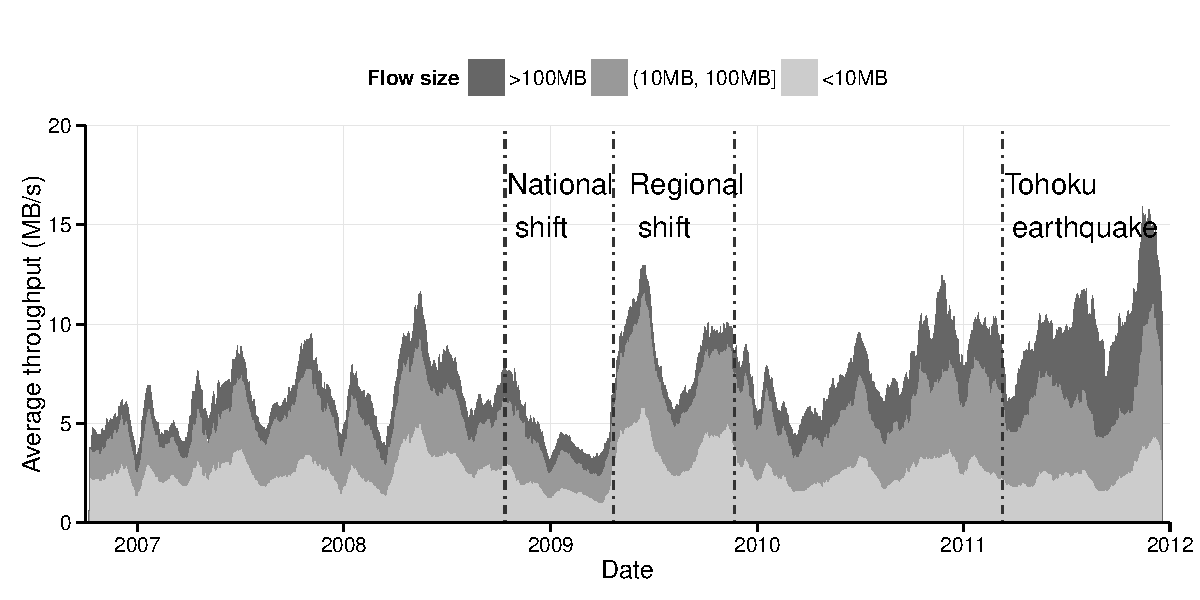
\includegraphics[width=0.9\textwidth]{figures/malawi/tput}
  \caption{Mean throughput}
  \end{subfigure}
  \begin{subfigure}[b]{1.0\linewidth}
  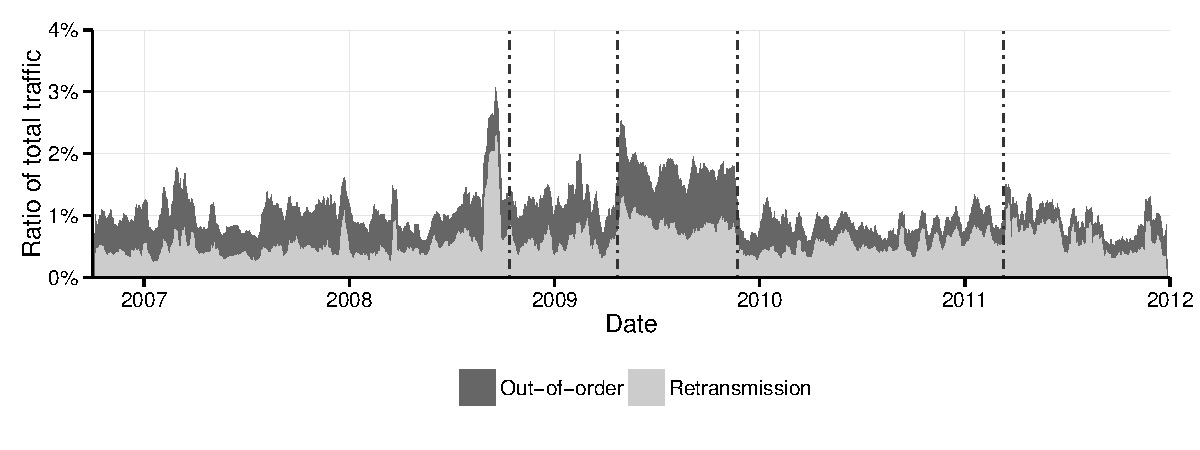
\includegraphics[width=0.9\textwidth]{figures/malawi/losses}
  \caption{Mean loss rate}
  \end{subfigure}
  \caption{Longitudinal evolution of inbound traffic.}\label{fig:MAWI}
\end{figure}

Over a five year period, changes in routing and application popularity have continually redefined the nature of traffic under observation.
This section provides a macroscopic view of these shifting trends. Figure \ref{fig:MAWI} displays the average throughput and loss ratio, calculated for TCP traffic only, smoothed on a weekly basis. 
Two routing changes internal to WIDE had significant impact on overall traffic, and are consequently highlighted.
The first, performed towards the end of 2008, diverted most of the inbound traffic from \emph{national} sources away from the monitored transit link, resulting in a reduction of traffic.
This event was preceded by increased congestion downstream from the monitoring point.
The second, in early 2009, saw a significant increase in \emph{regional} traffic from Asian neighbours, and was reverted approximately six months later. 
During this period aggregate end-to-end loss rates increased as a result.
While this is mostly due to the higher proportion of upstream congestion for traffic from Taiwan and China in particular, most traffic was adversely affected by the increased utilisation, suggesting that the transit link itself may have been a bottleneck during this period.
Finally, the impact of the Tohuku earthquake resulted in a noticeable break in demand coinciding with the start of the Japanese fiscal year in April, in which traffic traditionally ramps up.

\subsection{Geographic distribution}

\begin{table}\footnotesize
\centering
    \begin{tabular}{  
@{}
$>{\scshape}p{3.0cm}
^r
^r
^r
^r
^r@{\hskip 1.0cm}
^r
^r
^r
^r
^r
@{}
}
\toprule
\rowstyle{\scshape\bfseries}
\multirow{2}{*}{\parbox[][0.7cm][b]{3.0cm}{Country}} & 
\multicolumn{5}{c}{\scshape\bfseries{Outbound traffic (\%)\hspace*{0.45cm}}} & 
\multicolumn{5}{c}{\scshape\bfseries{Inbound traffic (\%)}} \\
\cmidrule(r{1.0cm}){2-6} \cmidrule{7-11}
\addlinespace[-0.6em] \rowstyle{\scriptsize\scshape}
 & 2007 & 2008 & 2009 & 2010 & 2011 & 2007 & 2008 & 2009 & 2010 & 2011 \\
\midrule

        United States & 27.3 & 31.3 & 29.3 & 36.4 & 35.7 & 45.7 & 41.5 & 53.3 & 65.1 & 67.1
\\
        \scriptsize{ California } & \scriptsize{ 39.0 } & \scriptsize{ 61.8 } & \scriptsize{ 63.5 } & \scriptsize{ 53.8 } & \scriptsize{ 50.6 } & \scriptsize{ 55.7 } & \scriptsize{ 47.9 } & \scriptsize{ 46.7 } & \scriptsize{ 24.9 } & \scriptsize{ 34.9 }\\\scriptsize{ Texas } & \scriptsize{  5.8 } & \scriptsize{  4.3 } & \scriptsize{  4.1 } & \scriptsize{  2.4 } & \scriptsize{ 13.9 } & \scriptsize{  7.0 } & \scriptsize{ 12.0 } & \scriptsize{  5.8 } & \scriptsize{  7.1 } & \scriptsize{  5.6 }\\\scriptsize{ Colorado } & \scriptsize{  1.9 } & \scriptsize{  1.2 } & \scriptsize{  0.6 } & \scriptsize{  8.5 } & \scriptsize{  2.8 } & \scriptsize{  4.9 } & \scriptsize{  6.0 } & \scriptsize{  5.9 } & \scriptsize{  9.7 } & \scriptsize{  5.8 }\\\scriptsize{ Virginia } & \scriptsize{  1.9 } & \scriptsize{  1.0 } & \scriptsize{  0.8 } & \scriptsize{  0.4 } & \scriptsize{  0.6 } & \scriptsize{  1.2 } & \scriptsize{  3.0 } & \scriptsize{ 14.1 } & \scriptsize{ 13.1 } & \scriptsize{  8.3 }\\\scriptsize{ Washington } & \scriptsize{  4.0 } & \scriptsize{  2.9 } & \scriptsize{  3.5 } & \scriptsize{  6.1 } & \scriptsize{  6.6 } & \scriptsize{  0.9 } & \scriptsize{  5.7 } & \scriptsize{  3.5 } & \scriptsize{  3.0 } & \scriptsize{  2.0 }\\\scriptsize{ New Jersey } & \scriptsize{  2.8 } & \scriptsize{  1.5 } & \scriptsize{  0.7 } & \scriptsize{  1.1 } & \scriptsize{  1.9 } & \scriptsize{  1.0 } & \scriptsize{  1.8 } & \scriptsize{  1.6 } & \scriptsize{  4.9 } & \scriptsize{ 13.6 }\\\scriptsize{ Massachusetts } & \scriptsize{  1.6 } & \scriptsize{  1.1 } & \scriptsize{  0.9 } & \scriptsize{  6.1 } & \scriptsize{  4.9 } & \scriptsize{  5.4 } & \scriptsize{  2.1 } & \scriptsize{  1.8 } & \scriptsize{  1.6 } & \scriptsize{  2.0 }\\\scriptsize{ Florida } & \scriptsize{  3.1 } & \scriptsize{  2.3 } & \scriptsize{  1.3 } & \scriptsize{  1.1 } & \scriptsize{  0.9 } & \scriptsize{  1.0 } & \scriptsize{  0.4 } & \scriptsize{  0.4 } & \scriptsize{  8.5 } & \scriptsize{  7.9 }
\\
        Japan & 11.6 & 15.4 & 17.7 & 16.7 & 16.1 & 33.8 & 32.2 &  7.3 & 8.1 & 11.5\\China &  7.9 & 20.5 & 17.8 & 10.3 &  5.9 &  2.5 &  5.3 &  6.3 & 4.6 &  3.1\\Korea, Republic of &  5.3 &  1.3 &  2.1 &  7.8 & 23.8 &  4.7 &  5.1 &  3.2 & 1.1 &  0.5\\Germany &  2.2 &  1.7 &  1.6 &  1.0 &  0.6 &  3.0 &  6.1 &  5.3 & 5.5 &  1.4\\Taiwan &  2.7 &  1.3 &  4.0 &  3.6 &  2.7 &  0.8 &  0.9 & 10.9 & 0.9 &  0.4\\Netherlands &  0.4 &  0.4 &  0.5 &  0.3 &  0.4 &  0.9 &  1.0 &  4.1 & 6.2 &  6.9\\India &  2.8 &  3.3 &  4.8 &  3.3 &  2.0 &  0.3 &  0.1 &  0.0 & 0.2 &  0.0\\France &  1.2 &  1.1 &  0.9 &  0.9 &  0.9 &  1.6 &  1.2 &  2.6 & 3.4 &  1.7\\United Kingdom &  1.1 &  1.0 &  1.0 &  0.9 &  0.7 &  2.5 &  2.2 &  1.6 & 1.3 &  1.3
\\
    \end{tabular}
  \caption{Percentage of inbound and outbound traffic by country\label{table:dest}. U.S. state values are relative to total national traffic.}
\end{table}



These changes are both visible in the geographic distribution of inbound traffic over time, shown in table \ref{table:dest}.
Prior to 2009, a significant proportion of transit traffic originated from within Japan. Over time, however, the ratio of traffic from Asia has been reduced. While this may foreshadow an increased concentration of traffic from the United States, it should primarily be viewed as a reflection of routing policy, with regional traffic being diverted to alternate routes as Japan became increasingly interconnected to its neighbours.


Further geographic shifts are apparent when breaking down US traffic by state.
The proportion of traffic originating from California has decreased over time, dropping from 55\% of total US traffic in 2007 to only 35\% in 2011.
In its place, a larger set of states have emerged as content providers, with New Jersey, Florida and Virginia contributing over a quarter of all traffic originating within the US by 2011.

%tip

Table \ref{table:dest} shows the geographic distribution of both inbound and outbound traffic since 2007. The majority of traffic flows to and from the United States, which has increased its share of bandwidth in either direction over the past five years. The proportion of traffic flowing from the United States is particularly high, accounting for almost 70\% of inbound traffic in 2011. While this may foreshadow an increased concentration of traffic within the United States, it should first be viewed as a reflection of routing policy, as regional traffic has been increasingly diverted to alternate routes. Inbound traffic from Japan, China, Korea and Taiwan have all been on the wane over the past five years as Japan has become increasingly interconnected to its neighbours. Of particular importance is the routing change at the end of 2008, which resulted in a sharp drop in inbound traffic from within Japan, with a net effect easily discernable in figure \ref{fig:inout}. This event had a profound influence in shaping not only the distribution of traffic, but also overall loss and delay as we shall observe in sections \ref{sec:delay} and \ref{sec:loss}.

A further point of interest is the breakdown of traffic from the U.S. by state. The overall increase in volume at a national level has broken the hegemony of California, which saw its overall share of inbound traffic fall from 60\% in 2007 to just under 40\% by 2011. In its place a larger set of states have emerged as content providers. Not listed are New Jersey, Florida and Virginia, which all saw sharp rises in 2011 to provide 35\% of all traffic from the U.S towards WIDE.
    
In the outbound direction, the geographic distrubtion of traffic is less skewed, with a greater proportion of traffic flowing towards Japan and China in particular. Due to a change in routing towards the end of 2010, traffic to Korea increases dramatically. In 2011, 12.7\% of all outbound traffic was destined to Korea Telecom alone. European destinations overall have a small proportion of outgoing traffic, which appears to be shrinking over time. The most significant factor for the discrepancy between inbound and outbound traffic for Europe as a whole is the timezone difference, as traffic is measured at 05:00GMT. This however does not account for why outbound traffic overall has been falling. Since most outbound traffic towards Europe at the time of measurement is likely to be scheduled transfers with no human intervention, a plausible explanation for this trend is the gradual shift away from file-sharing using peer-to-peer applications. This is further corroborated by the rise of hosting solutions which facilitate filesharing such as MediaFire, as shall become evident when analyzing the breakdown of traffic by AS.


\


\subsection{\acs{AS}-level distribution}
\begin{figure}
    \centering
    \begin{subfigure}[b]{0.5\linewidth}
        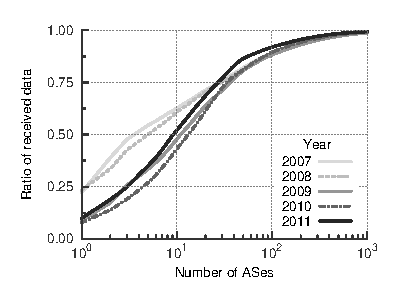
\includegraphics{figures/malawi/asn_cdf_in}
        \caption{Inbound}
    \end{subfigure}%
    \begin{subfigure}[b]{0.5\linewidth}
        \includegraphics{figures/malawi/asn_cdf_out}
        \caption{Outbound}
    \end{subfigure}%
    \caption{CDF of inbound data by AS. \label{fig:ecdf_asn_from}}
\end{figure}


%\begin{table*}\scriptsize
%\centering
%\subfloat[2007]{
    %\begin{tabular}{
@{}
$>{\raggedleft}p{0.6cm}
^>{\scshape}p{2.25cm}
^>{\raggedleft\arraybackslash}p{0.6cm}
@{}
}
\toprule
\rowstyle{\scshape\bfseries}
\acs{ASN} & \acs{AS} name &
\% \\
\midrule

    %\input{data/malawi/asn2007.tex}
    %\end{tabular} % closes asnheader.tex tabular environment
    %}
%\subfloat[2009]{
    %\begin{tabular}{
@{}
$>{\raggedleft}p{0.6cm}
^>{\scshape}p{2.25cm}
^>{\raggedleft\arraybackslash}p{0.6cm}
@{}
}
\toprule
\rowstyle{\scshape\bfseries}
\acs{ASN} & \acs{AS} name &
\% \\
\midrule

    %\input{data/malawi/asn2009.tex}
    %\end{tabular} % closes asnheader.tex tabular environment
%}
%\subfloat[2011]{
    %\begin{tabular}{
@{}
$>{\raggedleft}p{0.6cm}
^>{\scshape}p{2.25cm}
^>{\raggedleft\arraybackslash}p{0.6cm}
@{}
}
\toprule
\rowstyle{\scshape\bfseries}
\acs{ASN} & \acs{AS} name &
\% \\
\midrule

    %\input{data/malawi/asn2011.tex}
    %\end{tabular} % closes asnheader.tex tabular environment
%}
%\caption{
    %\label{table:topASin}
    %Top 10 ASes for inbound traffic by year. Additionally listed is the ratio of aggregate end-to-end loss.}
%\vspace{-3mm}
%\end{table*}


These large-scale changes are a natural outcome of content consolidation. This is most apparent at the AS level, where a direct mapping to a commercial entity is forthcoming.
Figure \ref{fig:ecdf_asn_from} shows the cumulative distribution of inbound traffic by AS, while table \ref{table:topASin} lists the top ten AS by traffic volume for 2007, 2009 and 2011.
While in 2007 traffic was already consolidated across a small set of ASes, a significant portion of transit traffic was Asian: most traffic from NTT and Limelight originated from within Japan. Such traffic has gradually been pushed away from transit by 2011.
Large carriers such as Cogent, Level3, Hanaro, China Telecom have also seen their importance diluted by ASes known to harbour one-click hosting services such as Choopa, Webazilla, WZ Communications, Carpathia and LeaseWeb.
Many of the hosted websites facilitate the distribution of copyrighted content, and as such are not capable of growing large enough to expand beyond hosted infrastructure without risking prosecution.
% overall summary: content consolidation, delay, etc
Overall, the observed traffic patterns match the insights provided by Labovitz et al. on the changing nature of interdomain traffic in \cite{Labovitz:2010p175}.
The implications for transit traffic from an Asian perspective is less intuitive: with the increased adoption of content delivery networks and internet exchanges points, more transit traffic is being retrieved from further away as content in the US shifts east.


%tip
It has been widely noted that inter-domain traffic has significantly changed over the past decade, with an increasing proportion of traffic flowing to and from a dwindling set of both large content providers and consumer networks. 
This shift carries potentially significant ramifications for network operators. 
Content consolidation provides opportunities for network optimization as a wider set of traffic is contained within a smaller set of addresses. 
Improved transport heuristics or dynamic traffic engineering are both feasible solutions under such conditions if designing for the typical case, rather than the worst case \cite{Dukki}.

Traffic consolidation is most apparent at the AS level, where a direct mapping exists to a commercial entity. 
How this translates down to the network layer is less clear. 
We start by investigating how traffic is distributed by both AS and network prefixes for inbound traffic, as shown in figure \ref{fig:ecdf_from}. 
Over the past five years, traffic has remained consistently concentrated in the top 100 ASes, accounting for approximately 90\% of all data received. 
Between 2008 and 2009, traffic to NTT (AS2914) dropped significantly as a wide range of Japanese prefixes were rerouted through a different ingress. 
Additionally, traffic from Limelight ceased to be visible from our measurement point. 
Together, they contributed over 30\% of all inbound traffic in 2007 and 2008. 
This explains the discrepancy in distribution between 2008 and 2009.

For outbound traffic, shown in figure \ref{fig:ecdf_to}a, consolidation has been much more perceptible. 
For the top 10 ASes alone, the proportion of traffic has more than doubled between 2007 and 2011. 
By 2011, the distribution of traffic amongst ASes for inbound and outbound traffic bears a striking similarity. 
The nature of this concentration is markedly different however, as made apparent by the distribution of traffic over network prefixes. 
The one hundred most popular network prefixes contribute 75\% of inbound traffic, yet only account for 50\% of outbound traffic. 
This matches our expectations on the inherent differences between large ISPs, which reflect the heterogeneity of their customer base through addressing, and content providers and CDNs concentrating resources in fewer locations. 



To further highlight this trend we display the top 10 ASes for both inbound and outbound traffic for 2007 and 2011 in tables \ref{table:topASout} and \ref{table:topASin} respectively. For each table we list the number of observed networks - networks belonging to that AS to which traffic was routed to over the entire year - the number of network prefixes which belong to the top 10000 networks and the ratio of traffic. Additionally, we display the values of the latter two values for prefixes with mask values greater than 19.

    For inbound traffic, both large consumer networks and content providers coexist in 2007. Youtube, Limelight, Google, Akamai and AcroNOC all send traffic almost exclusively from smaller address blocks. Additionally, most observed networks are amongst the highest ranked prefixes for inbound traffic, as opposed to large providers like NTT and Cogent, who have a much larger set of address blocks, but many of which do not have significant traffic. By 2011, NTT is the only ranked AS which still exhibits such behaviour for inbound traffic.

    Outbound traffic differs in many respects. Firstly, traffic was much less concentrated in 2007, with top ranked Google receiving a mere 3.6\% of all traffic. The remainder of the list is mostly compromised of large providers receiving most traffic through less specific prefixes. Curiously, NTT displays different patterns between inbound and outbound traffic, with a tendency to send from less specific prefixes, and receive to more specific ones. 

    In 2011 Korean telecom company KIXS exhibits a similar behaviour.  %WHY ??

    In this section we have shown how traffic consolidation has occured at different paces depending on the direction of traffic. Inbound traffic already showed strong signs of concentration in 2007, whereas outbound traffic has become dominated by large consumer networks and regional providers over the past five years. For both cases, traffic has converged towards similar distributions when analyzed by autonomous system, but the impact on routing seems markedly different. We will next focus on how these trends affect end-to-end traffic.


\subsection{Delay}
 
While understanding where traffic flows to and from is of great value at an operational, commercial and often political level, it portrays a small part of a wider picture. 
For end-users it is of less concern where content is being retrieved from or routed through compared to how long it takes.

\begin{figure}
    \centering
    \begin{subfigure}[b]{0.5\linewidth}
        \includegraphics{figures/malawi/rtt_cdf_in}
        \caption{Inbound}
    \end{subfigure}%
    \begin{subfigure}[b]{0.5\linewidth}
        \includegraphics{figures/malawi/rtt_cdf_out}
        \caption{Outbound}
    \end{subfigure}%
    \caption{CDF of RTT by AS. \label{fig:rtt_cdf}}
\end{figure}

\begin{figure}
    \centering
    \begin{subfigure}[b]{0.5\linewidth}
        \includegraphics{figures/malawi/rtt_wcdf_in}
        \caption{Inbound}
    \end{subfigure}%
    \begin{subfigure}[b]{0.5\linewidth}
        \includegraphics{figures/malawi/rtt_wcdf_out}
        \caption{Outbound}
    \end{subfigure}%
    \caption{CDF of weighted RTT by AS. \label{fig:rtt_wcdf}}
\end{figure}

The respective cumulative distribution functions of delay is display in figure \ref{fig:rtt_ecdf}. As with traffic distributions, the plots once again illustrate the same overall trend in subtly different patterns. Overall, delay has been decreasing over time, with the notable exception of a small segment of inbound traffic for network prefixes, mostly based in Japan, which were rerouted at the end of 2008. The rate at which delay has improved however seems markedly different. 

Comparing plots at the AS granularity, for the top 400 ASes delay has dropped by 20ms between 2009 and 2011 for inbound traffic, while the equivalent decrease for outbound traffic has been closer to 50ms. The absolute values in both cases are still disparate: over 90\% of ASes are reached within a round trip time of approximately 400ms when ranked by inbound traffic, whereas the equivalent value for outbound traffic is almost 200ms higher. This same trend is apparent when looking at delay by network prefix.

For inbound traffic the average RTT is low enough that geographical properties are clearly visible. A first plateau close to 100ms is apparent for traffic to the american west coast, while traffic to european destinations is clustured close to 250ms. Tellingly, this second plateau seems to be receeding in both AS and network plots. When taken in conjunction with the geographic distribution of traffic presented in table \ref{table:dest} this seems to confirm our suspicions that there has indeed been a reduction in the number of sources within Europe. 

A pertinent question at this point is in trying to understand how delay relates to traffic volumes. Given the different nature of stakeholders monopolizing traffic at either end of the spectrum, what can we say about the evolution of delay in either case? To assess this we plot the cumulative distribution of the average RTT weighted by the respective volume of traffic, as shown in \ref{fig:wrtt_ecdf}. In interpreting such plots one should keep in mind that they provide a rough indicator of the average delay to be expected if one were to sample a packet belonging to the top $N$ sources or destinations. As $N$ increases, we will approach the average RTT for all traffic in a given direction.

Inbound traffic by AS highlights and expected rise in delay between 2008 and 2009, as both NTT and Limelight are replaced by more distant sources. However, from 2009 onwards the overall delay is remarkably similar. While the cumulative distribution function of RTT shows improvement in delay at the tail, this results in very little improvement overall as traffic is dominated by a handful of entities.

Focusing on inbound traffic by network prefix not only confirms this, but actually shows that average delay has increased consistently over time.
In this case, the cumulative distribution of delay from \ref{fig:rtt_ecdf}b improved between 2009 and 2011, yet the average weighted RTT increased almost twofold for the top 10 network prefixes over the same period.

Two explanations emerge for this behaviour. The first stems from the changing nature of the traffic we are sampling. While functionally NTT represents the same entity over time, the traffic we observe is very different. As local traffic has increasingly been exchanged over peering links our view of traffic has stretched further afield. To illustrate this, one needs only notice that the average delay towards NTT, the top AS for inbound traffic in both 2007 and 2011, increased by approximately 100ms in figure \ref{fig:wrtt_ecdf}a. This does not represent a degradation in quality of service, but rather a change in where traffic is flowing from within the AS.

A further reason relates to the placement of content. As we had previously shown in \ref{table:dest}, there appears to be a migration of content away from California. Hosting sites such as Lemuria (Hotfile), based in Florida, Mediafire, based in Texas and District of Columbia and Carpathia, based in Virginia, are all contained within the top 20 ASes and have shifted traffic further from locations which had traditionally benefitted from low latency as viewed from Japan.

Analyzing the outbound traffic we seemingly get the opposite effect, with the average weighted RTT for the top 1000 ASes dropping by over 100ms. Once more, there is no single reason which accounts for the entirety of this effect. In 2007 many of the top destination ASes were in developing Asian countries, where infrastructure has improved greatly since. Improvements in routing to countries such as China and Korea have also had a positive net effect. This is visible in figure \ref{fig:rttyearcomp}, where the average RTT aggregated by country is plotted. For clarity, we filter out countries for which RTT estimates are available for less than 50 days in a year. Between 2007 and 2009 most Asian and European countries experience significant improvements in RTT. Those which don't tend to experience lower delays. Between 2009 and 2011 most countries reduce delay below 500ms. 

Finally, many of the very same companies which have had an effect of increasing RTT for inbound traffic, such as Mediafire or Ustream.tv, are also amongst the top destinations of traffic. It is interesting to note that as of 2011, data travelling from the top 1000 AS traffic sources is expected to experience the same latency as data travelling towards the 1000 most popular AS traffic destinations. In 2007, the value was two times higher for outgoing traffic.


\begin{figure}
    \centering
    \begin{subfigure}[b]{0.5\linewidth}
        \includegraphics{figures/malawi/rtt_comp_07_09}
        \caption{Inbound}
    \end{subfigure}%
    \begin{subfigure}[b]{0.5\linewidth}
        \includegraphics{figures/malawi/rtt_comp_09_11}
        \caption{Outbound}
    \end{subfigure}%
    \caption{CDF of weighted RTT by AS. \label{fig:rtt_comp}}
\end{figure}


\section{Performance Analysis}
%4.1) Balancing between two paths with high loss using fixed time unit
% using only loss-based balance in a simple regime where that works.
% Show how this converges quickly when one path suddenly gains
% background traffic (and hence loss).
%4.2) Balance between several paths with high loss and fixed time unit
% in simple regime where that works.
%4.3) Introduce experiment where equi-path is needed for probing and
% conservative is needed for low loss regime.
%4.4) Introduce experiment where time-scale tuning is needed to get
% good assessment of loss in low traffic regime.

This section evaluates \ac{PREFLEX} through simulation using ns-3 \cite{ns3}. 
Evaluating traditional traffic engineering methods typically involves abstracting traffic as flow aggregates, making large scale network performance analysis tractable.
\ac{PREFLEX} however balances traffic using loss rather than load, and focuses on improving end-user metrics as opposed to minimizing maximum link load.
As such, evaluating the proposed congestion balancer requires simulating end-to-end behaviour of traffic.

\subsection{Methodology}
\label{section:methodology}

Experimental validation is performed using the network topology displayed in figure \ref{fig:topo}. 
The topology links a client domain $C$ to a server domain $S$ through $N$ paths with equal bottlenecks $L_i$, and total bandwidth $B=\sum{L_i}$. 
While a domain is represented as a single entity in figure \ref{fig:topo}, each domain is composed by a traffic generator connected to a router. 
Client $C$ generates $G$ simultaneous \ac{HTTP}-like requests (or ``gets") from $S$ according to a specified distribution, described at the end of this section. 
As traffic flows from $S$ to $C$, the router within $S$ is responsible for balancing traffic over all available paths.

\begin{figure}
    \centering
    \includegraphics[width=2.5in]{figures/cate/topo}
    \caption{Simulation topology}
    \label{fig:topo}
\end{figure}

Across simulations, as the number of paths increases, total bandwidth $B$ and the number of simultaneous requests $G$ is fixed, providing insight into how efficiently \ac{PREFLEX} balances traffic as the granularity with which it can split traffic becomes coarser.

In order to evaluate how \ac{PREFLEX} shifts traffic in response to loss, additional ``dummy" servers $D_i$ are connected to $C$ through bottleneck link $L_i$.
The simulation runs for time $T$ and is partitioned into $N+2$ intervals starting on $s_i$, in which $s_0$ and $s_{N+1}$ have no traffic to $D_i$. 
Starting at time $s_i$, client $C$ generates $g_i$ requests to $D_i$ according to the same distribution as used to server $S$. 
All requests to $D_i$ end at time $s_{N+1}$. 
Equation \eqref{eq:si} sets the start time $s_i$ for requests to $D_i$ as a function of total simulation time $T$ and number of paths $N$. 
Likewise, equation \eqref{eq:gi} sets the number of simultaneous requests $g_i$ to $D_i$ as a function of $G$, the total number of requests to $S$, and $N$.
\begin{equation}
s_i = T\frac{i}{N+2}
\label{eq:si}
\end{equation}
\begin{equation}
\theta_i = \frac{\frac{1}{N+1-i}}{\sum{\frac{1}{N+1-i}}},  g_i = G\theta_i.
\label{eq:gi}
\end{equation}

Figure \ref{fig:demand} illustrates the number of simultaneous gets from $C$ to $D_i$ for $N=2$ (used in the example shown in figure \ref{fig:two}) and $N=4$. 
Generating cross-traffic in this manner serves two purposes. 
Firstly, $\sum{g_i}=G$, so independently of the number of concurrent paths, the maximum load in the system is $2G$. 
However, as the number of paths increases, the fluctuation in load for each path becomes smaller, stressing the sensitivity with which \ac{PREFLEX} must balance traffic. 
Secondly, the number of requests for each $D_i$ over time is the same. 
Over timescale $T$, equalisation appears to be an acceptable strategy but will however be shown to fail to make efficient use of available capacity. 
This is a fundamental limitation of offline traffic engineering, which is calculated over very long timescales and is unable to adapt as traffic routinely shifts.

\begin{figure}
    \begin{subfigure}[b]{.5\linewidth}
        \centering
        \includegraphics[width=2.25in]{figures/cate/dummy2-crop.pdf}
        \caption{$N=2$}\label{fig:1a}
    \end{subfigure}%
    \begin{subfigure}[b]{.5\linewidth}
        \centering
        \includegraphics[width=2.25in]{figures/cate/dummy4-crop.pdf}
        \caption{$N=4$}\label{fig:1b}
    \end{subfigure}
    \caption[Number of requests to cross traffic servers.]{Number of requests from $C$ to cross traffic servers $D_i$ for different values of $N$}
    \label{fig:demand}
\end{figure}

The settings used for all simulations, including those previously shown in figure \ref{fig:two}, are as follows.
Total simulation time $T$ is set to $1200$ seconds, while total bandwidth $B$ is fixed at $240$Mbps. 
The number of requests $G$ sent from $C$ to $S$ is set to 240. 
Upon completing, a request is respawned after an idle period following an exponential distribution with a $15$s mean. 
Transfer size follows a Weibull distribution with an average value of $2$MB. 
While artificial, these values attempt to represent traffic to a single prefix with a file size that mimics the small but bursty nature of web traffic, which does not lend itself to being balanced by the end-host. 
\ac{PREFLEX} is configured with $\beta_E = 0.05$, $\mu_{min}=0.01/N$ and $\delta=0.005$.

\subsection{Varying bottleneck distribution}

For the remainder of this section, congestion balancing using \ac{PREFLEX} will be directly compared to equalisation, which mimics existing traffic engineering techniques based on hashing flow tuples for path assignment.
A useful reference point in interpreting results is to examine the case where all bottlenecks share the same bandwidth, $L_i=B/N$.
Under such conditions, figure \ref{fig:goodputeq} shows the goodput, calculated as the total data transfered to client $C$ by flows completed within $T$, as a proportion of total link bandwidth.
The bulk of goodput originates from server $S$, which is the only multi-homed domain.
If traffic is correctly balanced, servers $D_{1-N}$ should generate the same amount of goodput.
While both equalisation and congestion balancing saturate most available bandwidth, the former leads to disproportionate distribution of goodput amongst competing traffic. 
As loss is not equalised over all paths, the amount of goodput achieved by servers $D_i$ differs despite demand being similar.
\begin{figure}
    \centering
    \includegraphics[width=4in]{figures/cate/eqbw}
    \caption[Goodput achieved over equal capacity links.]{Goodput relative to $B$ achieved by each server over equal capacity links.}
    \label{fig:goodputeq}
\end{figure}

In this scenario, equalisation can be seen as the optimal static TE solution, yet both approaches bear similar performance. 
With no knowledge of topology, link bandwidth or expected traffic matrices, \ac{PREFLEX} is able to adequately mimic the performance of the static TE solution for the case where such an approach is best suited.

\begin{figure}
    \centering
    \includegraphics[width=4in]{figures/cate/diffbw}
    \caption[Goodput achieved over unequal capacity links.]{Goodput relative to $B$ achieved by each server over unequal capacity links.}
    \label{fig:goodputdiff}
\end{figure}

Where bottleneck bandwidth is unequal however equalisation is shown to be severely lacking.
The effect of differing bottlenecks is investigated by repeating previous simulations with the same total bandwidth $B$, but with $L_i$ set proportionally to $B$ in a similar manner to \eqref{eq:gi}, that is $L_i = \theta_i B$.
The ensuing results, shown in figure \ref{fig:goodputdiff}, highlight two significant shortcomings of equalisation which \ac{PREFLEX} overcomes. 
Firstly, goodput for $S$ drops as $N$ increases. 
Unable to realize it is overloading a path, equalisation is reduced to sending traffic over each link at approximately the same rate as the most congested link. 
In contrast, \ac{PREFLEX} detects congestion and adapts accordingly. 
Secondly, the incorrect distribution of traffic due to equalisation in $S$ distorts the goodput of competing traffic. 
While in \ac{PREFLEX} goodput from $D_{1-N}$ is perfectly balanced, with equalisation traffic crossing the most congested links are directly affected by another domain's inability to distribute traffic appropriately.
It may seem unfair to judge equalisation for cases where there is a mismatch in link capacity.
However, such a mismatch between link weight and path capacity arises regularly as operators adjust traffic engineering according to local conditions, with little thought spared for the impact this may have further downstream.

\begin{figure}
    \centering
    \includegraphics[width=3.2in]{figures/cate/duration}
    \caption[Mean flow completion time.]{Mean flow completion time for equal and differing bottleneck links.}
    \label{fig:duration}
\end{figure}

This impact is in turn perceived by users, who experience longer flow completion times, as shown in figure \ref{fig:duration}. 
In the equal bandwidth case the flow completion time is similar for both balancers.  
Where bandwidth differs however, balancing by congestion outperforms equalisation and maintains a stable performance even for all six paths.  
This shows that the algorithm scales well as the number of available paths increases. 

\section{Closing the loop}

This chapter broadly describes an architecture which shares the responsibility for resource pooling between end-hosts and edge networks, but does not explicitly dictate an outcome. \ac{PREFLEX} has been designed to take into account the inevitable tussle which will occur between both, and envisages use cases where control over resource pooling could feasibly shift entirely in one direction or the other. 

At its most liberal, \ac{PREFLEX} enables resource pooling to be entirely performed by end-hosts. At its most conservative, \ac{PREFLEX} affords edge network providers more fine-grained control over traffic than before. Between either extreme, the resulting mutualistic architecture offers greater transparency, control and robustness by realigning the interface between network and transport in order to accommodate the needs of both.

In order to make \ac{PREFLEX} deployable, the scope of the architecture has been restricted to stub domains.
While this necessarily reduces the amount of path diversity which can be explored, there are compelling reasons to abdicate some flexibility in favour of a more practical solution:

\begin{itemize}
\item{
    \textbf{Most benefit derives from a limited set of paths}.
    Work on source routing \cite{Gummadi:2004p131,Yang:2006p405} suggests most improvement in resilience can be extracted from a small set of deflections.
    Stub domains such as \acp{ISP} and enterprise networks are naturally multi-homed, and can provide reasonable path diversity given an adequate selection of providers.
    Expecting the establishment of cross-domain paths has been a pitfall for previous research in \ac{QoS} in particular and is marred by difficulties in providing incentives for all parties involved.
}
\item{
    \textbf{Stub domains are most aligned with user interests}. 
    For enterprise, academic and content distribution networks, end-hosts are typically managed by the same entity which operates the network.
    For \acp{ISP}, there is a binding contract between end-users and provider.
    In either case, the stub domain not only benefits from not deteriorating the quality of service provided to hosts locally, but also has an interest in making sure end-to-end traffic is unaffected by outages or degraded performance.
    The inability to reach a website is often misdiagnosed by users as a failure of the stub domain, rather than the intervening network path or the remote host.
    As a result, the burden of remote failures is often placed on local customer support.
    \ac{PREFLEX} allows resources not only to be shared more efficiently, but also potentially reduces the impact of remote network events on stub domains.
}

\item{
    \textbf{The Internet topology is flattening}. 
    In studying over 100 \acp{ISP}, transit providers and content providers for over two years, Labovitz \emph{et al.} \cite{Labovitz:2010p175} established the changing nature of the Internet topology, migrating from a hierarchy of providers to an increasingly interconnected model.
    The rise of \acp{IXP} where customer networks peer directly with content providers has had a profound impact in shaping traffic patterns and interdomain traffic in particular.
    The length of \ac{AS} paths has decreased for most \emph{content}.
    As a consequence, it has become simpler for a stub domain to ensure path disjointness as a larger portion of the end-to-end path is under its control.
}
\end{itemize}

The resulting architecture provides many benefits. 
Balancing is both transport agnostic and allows flow state to be kept to a minimum, requiring policing at the edges only if congestion accountability is required. 
Additionally, path selection is receiver driven, aligning the stakeholder who can decide when to issue \ac{FNE} packets with the stakeholder who benefits the most. 
The key to path selection is the information provided by the sender (point 7 in figure \ref{fig:preflexout} ), which allows the network to estimate path loss on the same timescale as hosts. 
By pooling loss information from multiple hosts, the network may additionally be made aware of path failures sooner than hosts using \ac{TCP} inference.

%We assume for the entirety of this section that each flow follows a single path and that a host does not override the path selected by its network, although neither is strictly necessary. 
%The implications of both assumptions being broken and the incentives involved are briefly reviewed in \cite{Araujo:2010p224}.


\chapter{A longitudinal analysis of \acs{TCP} traffic}
\label{chapter:malawi}

\renewcommand{\locfolder}{\chapfolder/malawi}
While the Internet has become evermore interconnected, exploring path diversity has been relegated to an afterthought in an architecture modeled around assumptions that no longer stand. 
Single-path forwarding as a paradigm arose not as a guiding principle, but as a natural aversion towards increasing both the complexity and cost of a resource starved network.
%engineering for scarcity worked, but cracking
Engineering for scarcity has propelled the Internet to an unprecedented scale, but problems arise when what was otherwise scarce becomes plentiful. 
Protocols designed to be bit conservative at the expense of latency have become technological anachronisms as bandwidth costs continue to plummet. 
Similarly, the notion of a router as a device merely capable of forwarding packets has long been obsolete as Moore's law continues to pave the way for greater functionality within the network. 
\ac{NAT}, \ac{DPI} or \ac{PEP} are all examples that when it comes to drawing a boundary between network and transport, the line begins to blur \cite{Ford:2008p34}.

%% paralelism increasing
Furthermore, parallelism seems to be a dominant trend at every level of the Internet architecture as a cost-effective means of increasing both performance and robustness. 
At the inter-domain level, the \ac{AS} graph is becoming flatter and more highly interconnected \cite{Haddadi:2010p129}. 
Within domains, the sheer complexity of managing paths has led to the streamlined design and deployment of \ac{MPLS} \cite{Rosen:2001p147}, implementing a fully fledged layer in its own right. 
At the edges the rise in multi-homing continues to increase the strain on an already overloaded routing architecture. 
Even within network components, parallelism is such that packet re-ordering can no longer be considered pathological \cite{Bennett:1999p120}.

Given these trends, one would expect the ability to pool traffic across such emergent path diversity to have become a network primitive. 
In reality, each stakeholder in the Internet architecture seems to balance traffic according to their needs while attempting to remain inconspicuous to others. 
At best, this interaction between stakeholders can be seen as a form of commensalism, where one entity can extract benefits while others remain unaffected. 
At worse, the competitive nature of the tussle \cite{Clark:2005p67} that ensues can spiral into a situation where few profit.

This chapter investigates the nature of this antagonism between network and endpoints and reflects on how the Internet can accommodate the needs of both through the use of \ac{PREFLEX}, a proposed architecture for balancing congestion which foments mutualism between end-hosts and edge network providers.

\section{Related work}
\label{section:malawi:related}

Despite their inherent value, longitudinal studies of Internet phenomena are rare. 
Over its short lifespan the Internet has been shaped as much by technological change as by political and commercial realities. 
This dynamic nature does not lend itself to observational studies where data must be collected and curated over long periods of time, and has resulted in a scarcity of relevant datasets. 
What few exceptions exist often stem from collaborative research efforts, such as CAIDA \cite{CAIDA} or Oregon Routeviews \cite{routeviews}. 
The usefulness of these datasets however can be severely affected by the need for data privacy. 
The dissemination of interdomain routing information, where no such requirement exists, has assisted in a wealth of research on wide ranging topics, from quantifying path diversity \cite{Oliveira:2009p203} to locating Internet bottlenecks \cite{Hu:2004p96}. 
In contrast, longitudinal datasets relating to passive measurements have nurtured a much smaller community of researchers often focusing on characterizing traffic \cite{Fontugne:2010p413}. 
Stripped of the locality contained within IP addresses however, researchers are left unable to relate these findings to a wider context.
Instead, cross-sectional studies characterizing traffic aggregated by location are frequently conducted under different contexts \cite{Ager:2011:WCC:2068816.2068870}, but lack the temporal perspective only longitudinal studies can afford. 
Efforts to characterize the spatial properties of traffic over time \cite{Dhamdhere:2011p428,Labovitz:2010:IIT:2043164.1851194,Cho:2008:OSC:1544012.1544024} have defined the changing of Internet topology and traffic alike but fall short of relating such shifts with their impact on relevant metrics such as loss or delay. 

% other work since
This chapter builds on a wealth of prior work on understanding Internet traffic and serves as a reappraisal of significant past contributions.
Flow characteristics and \ac{TCP} behaviour at large are subject to frequent reassessment \cite{Zhang:2002p85}.
Of particular relevance to the current work are passive studies which delve into the inner mechanisms of \ac{TCP}.
In \cite{Jaiswal:2004p242}, Jaiswal et al.\ infer the sender's congestion window by identifying the congestion control variant from the behaviour observed during loss recovery.
The use of separate state machines for each variant however proves unscalable given the many flavours of \ac{TCP} congestion control which have since been deployed.
In \cite{Lan:2006p566}, Lan et al.\ analyse flows according to size, duration, rate and burstiness and characterise the observed correlations for heavy-hitters specifically,
uncovering evidence of increased application influence on flow rates and burstiness and consequently suggest treating flow size and duration as independent dimensions.

One central aspect to the analysis of \ac{TCP} behaviour is the estimation of \ac{RTT} from packet capture data. 
In addition to SYN-based methods, Shakkotai et al.\ \cite{Shakkottai:2004p408} evaluate further techniques to estimate the \ac{RTT} of a unidirectional flow. 
The \textit{rate change} method establishes a relation between the \ac{RTT} and the increase in sending rate, assuming linear window increases during congestion avoidance. 
Unfortunately, this assumption no longer holds, both due to the proliferation of less conservative congestion control algorithms such as CUBIC \cite{Ha:2008p471}, and due to application-driven flow control. 
An alternative is the use of frequency-domain techniques \cite{Veal:2005p412,Lance:2005p565,Qian:2009p429}, which are a natural fit given the self-clocking nature of \ac{TCP}. 
However, a common difficulty with the application of spectral analysis is extracting the fundamental frequency which corresponds to the \ac{RTT} in the presence of noise. 
In applying the Fourier transform to inter-packet arrival times, for example, Qian et al.\ \cite{Qian:2009p429} note that less than half of all flows have distinguishable \textit{flow clocks}; likewise, the \ac{FFT}-based \ac{RTT} recovery was found to be unreliable even after pre-processing available data to enhance inherent periodicities.

% topological influence
Finally, it is important to elucidate what changes in traffic properties are intrinsic to \ac{TCP} and data transfer, and which ones arise from large-scale changes in the \ac{AS}-level topology of the Internet. 
In the decade since publication of \cite{Zhang:2002p85}, the Internet has undergone significant changes, shifting from a broadly hierarchical form to a flatter, more interconnected structure \cite{Labovitz:2010p175,Ager:2012p567}.
Given the longitudinal nature of this chapter and its focus on interdomain traffic in particular, the insights provided by these studies on the macroscopic effects of content consolidation are discernible within the studied dataset, and as such are a source of validation for many of the observations herein.

\section{Dataset}
\label{section:malawi:dataset}

This section provides an overview of the datasets used in this work and some of the data processing required before approaching the longitudinal study of Internet traffic rate limiting. 
The dataset used is composed from the original, un-anonymised traffic traces from the \ac{MAWI} dataset \cite{mawi}, a set of daily packet captures from the \acs{WIDE} backbone network which provides connectivity to universities and research institutes in Japan. 
Traffic is collected daily for 15 minutes starting at 14:00 \acs{JST}. 
Although this dataset extends back largely uninterrupted from late 2001, the present work focuses on just over five years of data following a network upgrade to the monitored link on October 2006.
The monitored link carries mostly trans-Pacific commodity traffic between \acs{WIDE} customers and non-Japanese commercial networks. 
Traffic towards \acs{WIDE} is referred to as \emph{inbound} traffic, whereas traffic originating from within \acs{WIDE} is referred to as \emph{outbound} traffic.

\begin{table}[!htp]
\footnotesize
\centering
\ra{1.2}
    \begin{tabular}{
@{}$ % cut edge, start row
>{\raggedright\arraybackslash}p{1.0cm} % year
^>{\raggedleft\arraybackslash}p{1.0cm}@{\hskip 1.0cm} % days
^>{\raggedleft\arraybackslash}p{1.7cm}@{\hskip 1.3cm} % flows
^>{\raggedleft\arraybackslash}p{1.0cm}                % traffic in
^>{\raggedleft\arraybackslash}p{1.0cm}@{\hskip 1.0cm} % traffic out
^>{\raggedleft\arraybackslash}p{1.0cm}                % AS 
^>{\raggedleft\arraybackslash}p{1.0cm}                % AS 
@{} % cut edge
}
\toprule
\rowstyle{\bfseries\scshape}
\multirow{2}{*}{ \parbox[][0.8cm][b]{0.5cm}{Year}} &
\multirow{2}{*}{ \parbox[][0.8cm][b]{0.5cm}{Days}} &
\multirow{2}{*}{ \parbox[][0.8cm][b]{2.5cm}{\centering TCP data \\ flows ($\times10^3$)}} &
\multicolumn{2}{c}{ \bfseries\scshape Traffic (TB) \hspace*{0.8cm} } & 
\multicolumn{2}{c}{ \bfseries\scshape Unique ($\times10^3$) } \\

\cmidrule(r{1.0cm}){4-5} \cmidrule{6-7}
\addlinespace[-0.6em] \rowstyle{\scshape\scriptsize}
& & & \centering In & \centering Out & \centering AS & Prefixes \\
\midrule

    2006 & 91 & 20.52 & 0.43& 0.45 & 10.90 & 56.86\\
2007 & 350 & 102.56 & 2.11 & 2.49& 17.21 & 113.79\\
2008 & 358 & 112.26& 2.43 & 2.10& 24.74 & 156.54\\
2009 & 364 & 113.97& 2.48 & 2.53& 19.71 & 143.87\\
2010 & 365 & 113.70& 2.58 & 3.43& 20.38 & 148.03\\
2011 & 358 & 114.74& 3.44 & 5.14& 19.99 & 140.56\\
\addlinespace[0.4em] \rowstyle{\bfseries}
Total & 1886 & 5777.55 & 13.50 & 16.14 & 34.12 & 341.22\\

    \bottomrule
    \end{tabular}
    \caption{\label{table:overview}Overview of traced \acs{MAWI} dataset.}
\end{table}

A preliminary overview of the dataset used is provided in table \ref{table:overview}. 
In total, 5.7 billion flows containing data are traced over five largely uninterrupted years; this represents approximately 30 terabytes of \ac{TCP} traffic. For the purposes of this work, most analysis will focus on inbound traffic, 60\% to 80\% of which originates from port 80, referring only to analysis of outbound traffic when contextualizing findings.
Given the sender side plays a critical role in shaping traffic, analysing traffic for which the source is restricted to a small set of networks within Japan is of limited use in accurately depicting traffic trends at large.
Hosts within Japan are instead fixed as traffic sinks, thus sharing a similar perspective on inbound traffic as many other similarly sized networks. 

\subsection{Tracing \acs{TCP} Metrics}

All \ac{TCP} flows are reassembled and analysed for each daily trace.
In addition to the five tuple used to define each connection, two additional restrictions are imposed: a contiguous sequence number space and a three minute timeout. 
These restrictions are helpful to deal with port reuse and unterminated flows respectively.  
Although the total number of \ac{TCP} flows increased dramatically in 2011, the number of flows for which data payload was observed has remained stable, averaging over 100 million data flows traced per year.  

There is much prior work with regards to reconstructing \ac{TCP} flow from passive measurements and using this information to understand the end-to-end properties of traffic \cite{firstRTT,Jaiswal:2007p233,Rewaskar:2007p195,Shakkottai:2004p408}. 
However, the \acs{MAWI} traces impose two constraints which require careful consideration, and ultimately led to the use of a custom \ac{TCP} tracer. 
The first is the proportion of bidirectional flows, where both forward and reverse path are seen. 
In the dataset used this fluctuates between 40\% and 60\% over five years.
Most available \ac{TCP} tracers either ignore or are inadequate at processing unidirectional flows. 
The second is the short duration of each individual trace file. 
At only 15 minutes of line-rate data capture per day, it is wasteful to ignore flows which are not complete. 
Although the number of flows for which a SYN and FIN in either direction is observed has remained consistently high until late 2011, these flows are normally \emph{mice}, i.e. flows that tend to be brief and which carry little traffic individually. 
In contrast, most \emph{elephants} (flows that carry significant traffic individually) have durations that exceed that of each trace file. 

Loss is inferred by accounting for \emph{retransmissions} in the upstream data and \emph{out-of-order packets} in downstream data; for the remainder of the paper the term \emph{end-to-end loss} will refer to the sum of out-of-order and retransmitted data bytes over the total data bytes in a given direction.
Anecdotally, this was found to be an adequate indicator of loss --- with the exception of \emph{hanging} \ac{TCP} connections. 
In such cases where connectivity is lost, a host will proceed to retransmit packets while performing an exponential back-off. 
Although this results in negligible overall traffic, it can significantly skew the inferred loss ratio for uncommon destinations for which little traffic exists. 
To account for these cases, a 3-second timeout on retransmissions was imposed, after which the congestion feedback loop is considered to be broken. 

Each daily trace in the dataset is processed from a packet level capture into a collection of flow level statistics, providing insight into the end-to-end characteristics of traffic. 
However, since a core objective of this work is to augment this time-based information with data describing the endpoints of each flow, aggregating by location is also required. 

\subsection{Aggregating by Location}

Location information is added by mapping the original source and destination \ac{IP} addresses to its geographical and topological counterpoints. 
The routeviews archives \cite{routeviews} are used to reconstruct the mapping between each \ac{IP} and both \ac{AS} and network prefix; bi-hourly dumps of \ac{BGP} \acp{RIB} are available in the \acs{WIDE} archives since mid 2003. 
A daily \ac{RIB} is reconstructed based on the views provided by contributing \acp{AS}, in particular \acs{IIJ} and \acs{APNIC}.
Since there is no record of local policy, exact routes are not disclosed and as such there is no prior knowledge of the route taken by packets; this however does not hinder the ability to consistently map \acp{IP} to \acp{AS}.
While discrepancies in \ac{AS} destinations exist between different routeviews contributors, this happens almost exclusively on prefixes for which no actual traffic is seen. 

Mapping \ac{IP} to country is done through the use of GeoLite \cite{maxmind}, a commercial geolocation database. 
While the accuracy of this solution is often disputed, locating traffic at a fine granularity is not a pressing concern.
Most geographic emphasis will be placed on capturing macroscopic shifts in time at a national level, for which Geolite proves adequate.
The archive for geolocation data only extends to 2009, before which the earliest match must be used.
Additionally, the administrative mapping up until mid 2009 for a destination or source \ac{AS} is verified to have remained the same in the relevant \ac{RIR} archives in order for a flow to be assigned a geographical location.
% bridging paragraphs to save space.
After associating flows to country, region, \ac{AS} and network prefix for both source and destination \acp{IP}, flow statistics are aggregated over each location identifier. 
This generates a daily collection of location identifiers and associated flow properties, from which the geographic and topological properties of the dataset can be sketched over time.

\section{Methodology}
\label{section:malawi:methodology}

Providing a macroscopic view on where traffic originates from, and in what quantity, can be achieved by simply binning packets into flows and accumulating byte counts over geographical or topological locations. 
Uncovering application layer characteristics (i.e. \textit{how} traffic is sent) is a more complex problem that requires additional methods to reverse engineer transport behaviour.
The aim of this section is to describe a process which distinguishes those flows which have their throughput limited by mechanisms other than the usual \ac{TCP} response to loss and delay.
Each flow can be characterized as being either application paced, in which the sending application is limiting the data provided, host limited, whereby local constraints at either end host cap throughput, or receiver shaped, in which an artificial constraint is imposed by either a middlebox or receiver.

The classification proceeds in stages. 
Before classification, if a flow is not bidirectional its RTT must be recovered.
This is achieved in section \ref{subsection:malawi:PeriodicEnhancement}. 
Because the sender's TCP state machine cannot be directly observed, the congestion window must be instead estimated by observing the number of unacknowledged bytes in flight (\textit{flight size}).
This reconstruction is described in section \ref{subsection:malawi:flightAggregation} and provides the basis for flow classification. 
Flows are then checked in turn to see if they are application paced, host limited or receiver shaped and classified as belonging to the first of these classes for which they fulfill the necessary conditions.
Flows in none of these classes are either limited only by the network (delay or loss conditions) or are insufficiently large for constraints to be reliably detected.

\subsection{\acs{RTT} Estimation}
\label{subsection:malawi:PeriodicEnhancement}

Building on prior work presented in section \ref{section:malawi:related}, this section proposes an algorithm that scalably recovers the RTT from one-directional traffic traces. 
% XXX: below implies microflights were used, but these aren't described (remove as appropriate)
Although \ac{RTT} estimation is a difficult problem, simplifying assumptions can be made.
For the \acs{MAWI} dataset most \acp{RTT} are relatively large, with the closest neighbouring country, South Korea, roughly 40ms away.
By only processing bidirectional traffic from Japan, the expected \ac{RTT} range can be reduced for all other traffic.
The recovery mechanism then enhances the natural periodicity of traces and scalably constructs flights associated with specific application and protocol behaviour.
In the following the mechanisms required by these two goals are described. 
%
% Why does this work?
%
In normal operation, many \ac{TCP} operations involve request-response cycles between two endpoints in which the \ac{RTT} $T$ provides a natural \emph{clock}.
Hence, the most natural way to estimate \ac{RTT} from \ac{TCP} traces is to correlate requests and responses exchanged in both directions. 
If only one direction of data is observed however, $T$ cannot be directly observed. 
Instead, it must be estimated from the way in which \ac{TCP} packets cluster in time due to the batching of request-response operations.

The \ac{TCP} \ac{cwnd} determines the number of unacknowledged bytes that a \ac{TCP} flow may maintain at any point in time. 
This can be referred to as \emph{bytes in flight} because they are in transit between the sender $S$ and the receiver $R$; an equivalent definition applies for the number of \emph{packets in flight}. 
Once $S$ has transmitted \ac{cwnd} data bytes, it will refrain from transmitting more until either some bytes are acknowledged by $R$ or \ac{cwnd} is increased by the sender. 
In the absence of losses, neither of these events can happen until a \ac{TCP} \ac{ACK} is received; this immediately reduces the number of unacknowledged bytes, but may also lead to a significant \ac{cwnd} increase (during e.g. \emph{slow start}). 
% XXX: number of unacknowledged bytes reduced, or CWND?
In the presence of losses, however, bytes can be re-sent if a packet is timed out and considered lost; in this case, the number of unacknowledged bytes is reduced.

%
% What is our main contribution, algorithmically speaking?
%
The main difficulty associated with one-sided TCP flow reconstruction is as follows.
Let $t_1, t_2, \ldots$ be a set of times at which packets $p_1, p_2, \ldots$ were observed at $S$ en route to $R$.
Suppose that a packet $p_j$ of size $b$ is observed at time $t_j$.
In addition, suppose that approximately one RTT $T$ later, the sender $S$ receives an ACK $a_j$ from $R$ for the $b$ bytes of $p_j$.
At this point, the TCP stack in $S$ will decrease the number of unacknowledged bytes by $b$, thus opening the possibility for sending additional traffic to $R$.
This can lead to another packet $p_k$ to be transmitted; let this packet be observed at time $t_k$ as it is sent towards $R$.
Assuming that processing delay is insignificant, the RTT experienced by $p_j$ can be approximated as $T \approx t_k - t_j$.
Now consider what happens if packets are only observed in the $S \rightarrow R$ direction.
Under such conditions, it is not possible to ascertain whether $p_k$ was sent explicitly as a result of $S$ receiving the unobserved \ac{ACK} $a_j$, or whether it was sent as a result of an \ac{ACK} $a_i$ associated with a previous packet $p_i$ rather than with $p_j$.
If, however, a packet $p_l$ is eventually observed that did result from the reception of $a_j$, the \ac{RTT} can be estimated as $T \approx t_l - t_j$ with $t_l > t_k$.
Following this same reasoning, approximately one \ac{RTT} later a packet $p_m$ will be observed for which $2T \approx t_m - t_j$; this can potentially continue for as long $S$ has data to send and $R$ continues sending \acp{ACK}.
This is the underlying reason that \ac{RTT}-related periodic regularities arise when considering the timestamps of observed packets \cite{Qian:2009p429}.

The reasoning above is at the heart of the proposed algorithm to improve \ac{RTT} recovery by enhancing packet stream periodicity. 
Assume that a packet $p_j$ is observed at time $t_j$. 
Considering the set $\mathcal{T}_j$ of all values of $\Delta t = t_k - t_j$ for every $k > j$, it is apparent that it will include estimates not only for the \ac{RTT} $T$, but also for all its multiples $2T, 3T, \ldots$ 
If $t_l-t_k \approx T$ and $t_k - t_j \approx T$ then it follows that $t_l - t_j = 2T$, and this value will also be included in $\mathcal{T}_j$. 

By maintaining a set $\mathcal{T}_j$ for every packet $p_j$ observed, at least some of its values will correspond to estimations of multiples of the \ac{RTT}. 
It then follows that by creating a set $\mathcal{T}$ that includes values calculated starting from every packet $p_j$ so that $\mathcal{T} = \cup_j \mathcal{T}_j$, numerous estimates for $2T, 3T, \ldots$ will also be included. 
Hence, the probability density function $H(t)$ of the values in $\mathcal{T}$ should show peaks around multiples of the \ac{RTT} (see Figure \ref{fig:histogram}). 

\begin{figure}
  \centering
  \includegraphics[width=0.8\textwidth]{figures/malawi/rttbin.pdf}
  \caption{$H(t)$ for flow displayed in Figure \ref{fig:hostlimited}. The horizontal line delimits $\overline{H}$ while the highlighted bin denotes the bidirectional RTT estimate.\label{fig:histogram}}
\end{figure}

%
% Explain why did we use FFT
%
The algorithmic recovery of $T$ from $H(t)$ presents additional challenges. 
In particular, $H(t)$ may include a large number of \ac{RTT} multiples, and a peak will be found for all of them. 
Crucially, all these peaks may be of comparable magnitude, complicating the task of selecting a single peak.
Moreover, these peaks need not be very pronounced, with histogram bins in close proximity of the peaks have very similar values as the peak itself. 
As such, taking \ac{RTT} candidates directly from $H(t)$ may result in a large set of similarly-valued bins situated around a peaks at multiples of the \ac{RTT}. 

Three recovery algorithms for $T$ are attempted.
First, as a baseline, the highest peak in $H(t)$ is selected as a candidate for $T$. 
In addition, expanding upon the work of Qian et. al. \cite{Qian:2009p429} a frequency-domain representation of $H(t)$ is used to identify $T$. 
This is done by selecting the highest peak of $|\hat{H}(\omega)|^2$, the \emph{energy spectral density} of $H(t)$ (i.e. the norm squared of the Fourier transform of $H(t)$). 
Finally, a custom utility-based technique that operates directly on $H(t)$ is proposed which achieves superior performance to both of the aforementioned methods.

%\subsubsection{FFT-Based RTT Recovery}
%We extract periodicity information from $H(t)$ by looking at $\hat{H}(\omega)$, the \emph{energy spectral density} of $H(t)$. Formally, $\hat{H}(\omega)$ is defined as the norm squared of the Fourier transform of $H(t)$, so that $\hat{H}(\omega) = |\mathcal{F}(H(t))|^2$. Using $\hat{H}(\omega)$ markedly improves the quality of our RTT estimation because the frequency peak corresponding to the RTT usually accounts for a much larger proportion of the total frequency domain energy than other peaks in $\hat{H}(\omega)$, leading to a much simpler discrimination of the true RTT. However, due to RTT changing during the lifetime of a flow, and also due to the expected noise associated with real-life data sources, $\hat{H}(\omega)$ can also occasionally include large peaks at frequencies unrelated to the RTT. In order to filter these out, we take a set of 10 frequency candidates from $\hat{H}(\omega)$, and use their associated periods as RTT candidates in our flow reconstruction algorithm (see Section \ref{
%subsection:malawi:flightAggregation}). We then select that RTT candidate which exhibits the smallest error, that is, that one which yields closest agreement with observed data.

%
% Algorithmic hacks
%
%To streamline our algorithm for streaming use, we use the following heuristics and approximations. Firstly, we define a range $[T_{\min}, T_{\max}]$ representing the range over which we find the RTT values of interest. Then, for each packet $p_j$, we build a subset $\mathcal{T}_j'$ of $\mathcal{T}_j$ by including all values of $t_j - t_k < T_{\max}$. We then generate $\mathcal{T}' = \cup_j \mathcal{T}_j'$ and approximate $H(t)$ by considering a histogram of the values in $\mathcal{T}'$. As usual, we do this by counting the frequency with which its values are observed in the ranges $[0,\tau)$, $[\tau, 2\tau)$, $[2\tau, 3\tau), \ldots$ where $\tau$ is the time resolution required. 


\subsubsection{Utility-Based RTT Recovery}
\label{sect:utilityBasedRecovery}

This method relies not on the identification of periodicities, but on explicitly matching experimentally found signatures. 
To this end, we consider the peaks of $H(t)$, which are then considered RTT candidates.  
However, trivial discriminators (such as simply selecting the highest peak) are not reliable. 
In this case, it was found experimentally that repeatable peaks and troughs also occur at multiples and sub-multiples of $T$, with the most important ones being $\frac{T}{3}$, $\frac{T}{2}$, $T$ and $2T$. 
We design this detection algorithm around the idea that a given pattern of peaks and troughs can identify $T$.

If we define $\overline{H}$ as the mean height of $H(t)$, we can define a per-peak utility function $p(t)$ so that 
\begin{equation*}
p(t) = 1.0 - \exp\left(-2.0 \left(\frac{H(t)}{\overline{H}}\right)\right) \mbox{.}
\end{equation*}
This function has several advantageous properties: it is 0 if $H(t)$ is zero, 1
if $H(t)$ is infinite, and $0.5$ if $H(t) = \overline{H}$.  In other
words it is a measure of the \emph{peakiness} of the data, with $p=1$ identifying
an infinitely high peak, $p=0$ identifying an empty histogram bin (trough), and $p=\frac{1}{2}$ 
implying that $H(t)$ is of exactly average height at that point. We can then score each candidate using the following utility function:
$$
P(t) = 1.5 p(t) + p(2t) - p\left(\frac{t}{2}\right) - p\left(\frac{t}{3}\right).
$$
That is, the candidate RTT $t$ scores highly if it is itself a peak, if it has a peak
at a multiple $2t$, and if it also manifests troughs at submultiples $\frac{T}{2}$ and $\frac{T}{3}$.
The factor of 1.5 was added after observations
showed that the peak at $T$ was the most important factor in determining
whether a candidate was the true RTT. Similarly, additional multiples and submultiples 
were excluded as they showed very limited discriminating power experimentally.

\begin{figure}
  \centering
  \includegraphics[width=0.8\textwidth]{figures/malawi/rttcomp.pdf}
  \caption{Accuracy of RTT estimator when compared to the median value of bidirectional estimate.}
\end{figure}

\subsubsection{Comparing RTT Recovery Algorithms}
\label{sect:comparingRecoveryAlgos}
As described in Section \ref{subsection:malawi:PeriodicEnhancement}, $H(t)$ is calculated in such a way that RTT periodicity is amplified. 
This means that FFT-based techniques could potentially perform better on $H(t)$ than on the packet stream with no pre-processing. 
However, this is complicated not only because $H(t)$ contains periodicities at multiples of $T$, but also discontinuities that generate harmonics at frequency multiples of the RTT fundamental. 
Hence, although the FFT $|\hat{H}(\omega)|$ of $H(t)$ is much cleaner than that of the packet interarrival time series on its own, its maximum peak rarely coincides exactly with the RTT clock (this corroborates reports by Qian et al \cite{Qian:2009p429}). 
Thus, applying the FFT leads to another \emph{peak detection problem} in which the RTT fundamental needs to be extricated from its harmonics and sub-harmonics. 
The trivial solution to this problem, the application of a bandpass filter around the RTT frequency, is of course unfeasible because the bandwidth and 
centring of such a filter depend on the RTT which is itself unknown.
The utility-based algorithm described in Section \ref{sect:utilityBasedRecovery} can hence be applied in either the time domain or the frequency domain; we chose to do it on the former on the interest of expediency and lower computational cost.

\newcommand{\RTTHeader}{Below & Above}
\newcommand{\SmallFlowName}{\textless 10MB}
\newcommand{\LargeFlowName}{\textgreater 10MB} 
\begin{table}
\footnotesize
\centering
\begin{tabular}{ p{1.5cm} p{1.2cm} p{0cm} p{.6cm}p{.6cm} p{0cm} p{.6cm}p{.6cm}}
& & & \multicolumn{2}{c}{Peak} & & \multicolumn{2}{c}{Utility-based} \\
\cline{4-5} \cline{7-8}
& Flow size & & \RTTHeader & & \RTTHeader \\
\cline{4-5} \cline{7-8} 
\multirow{2}{*}{Receiver side}  & \SmallFlowName && 4.31 & 9.13 && 4.58 & 6.35
\\ 
                                & \LargeFlowName && 6.72 & 6.43 & 4.97 & 5.33
\\
\multirow{2}{*}{Sender side}    & \SmallFlowName && 2.94 & 8.37 && 3.29 & 4.80
\\
                                & \LargeFlowName && 6.41 & 9.06 & 5.40 & 11.06
\\
\end{tabular}
\caption{\label{table:rttRecovery}Performance of RTT recovery algorithms}
\vspace{-3mm}
\end{table}

The performance of the analysed RTT recovery mechanisms is presented in Table \ref{table:rttRecovery}, that shows the percentage of total flows below and above the RTT range given by the bidirectional estimates.
We separate things for \emph{inbound} traffic (where we are positioned at the receiver side) and \emph{outbound} traffic (where we are positioned at the sender side). The utility-based algorithm is particularly useful to address RTT underestimation for flows over 10MB in size, which is our main objective since precisely that kind of estimation error would interfere with our ability to correctly decouple application behaviour from RTT-scale dynamics.


%For the most part, the utility based method improves on underestimation, which is our main objective since that would interfere with our flight reconstruction (i.e. generate lots of gaps).
%The exception (kind of) is traffic from the sender side, which in our training set (one week per year), had quite a lot of host limited traffic (paced out, no signal to recover).
%In this case, not a problem, since if the flow is long enough multiples of the RTT will still reveal host limitation, but will give us a smaller window..


\subsection{Flow Classification}
\label{subsection:malawi:flightAggregation}

One fundamental precondition to decouple the influence that network loss, host configuration and TCP behaviour has on the throughput experienced by a flow is the reconstruction of the congestion window behaviour of TCP flows on the basis of observed data. 
Unfortunately, the congestion window value is internal to the sender's TCP state machine and may not manifest itself in the absence of sufficient data from the application layer. 
A more easily observed quantity which serves as a reasonable proxy for the congestion window is the number of unacknowledged bytes in flight, henceforth referred to as the \textit{flight size}, which can be derived given an accurate estimate of the end-to-end delay.
The evolution of both flight size and RTT can in turn be used to ascertain to what extent throughput is regulated by limitations imposed at different layers of the networking stack.

% definitions
Given a candidate RTT, we can aggregate a stream of packets with arrival times $t_1, t_2, \ldots$ into a stream of \emph{flights}. 
Intuitively, a flight is a clustered subset of a TCP flow which exhibits its own temporal coherence; alternatively, it can be though of as a series of consecutive packets that were (roughly) generated by the sender as a response to the same protocol operation. 
A flight $f_i$ that begins
with the $j$th packet and ends with the $k$th is defined to have a \emph{total flight time} $\tau_i = t_{k+1} - t_j$. 
The algorithmic selection of initial and final packets in such a way that the resulting flights are indicative of TCP behaviour remains an open problem. 
Since we assume that the RTT provides a natural time frame for the operations of TCP, in the algorithm presented in this work, given an initial packet $\pi_j$ and an RTT estimate $T$, the $k$th (and final) packet is selected to minimise \emph{the flight time error} $e_i = |T - \tau_i|$. 
This mechanism follows closely the methodology described in \cite{Zhang:2002p85}, with the exception that we do not attempt to define flights as being both adjacent and disjoint; rather, we decompose flows into a stream of potentially overlapping flights. 
This helps the algorithm mitigate the deleterious effects of small deviations in the estimated RTT, which alters the properties of each flight. 
Furthermore, since the flight size is continuous in time, it makes little sense to restrict ourselves to a single sample per round trip time.

Having obtained flight information from each flow, we next consider what is the predominant factor that affects its throughput. 
Within the context of TCP, we classify flows as being artificially constrained by three distinct processes: \emph{application pacing}, \emph{host limited} and \emph{receiver shaping}.

\begin{figure}
\centering
  \centering
  \begin{subfigure}{1.0\linewidth}
    \includegraphics[width=1.0\textwidth]{figures/malawi/youtube.pdf}
    \caption{Application paced. \label{fig:youtube}}
  \end{subfigure}\\
  \begin{subfigure}{1.0\linewidth}
    \includegraphics[width=1.0\textwidth]{figures/malawi/hostflow.pdf}
    \caption{Partially host limited. \label{fig:hostlimited}}
  \end{subfigure}\\
  \begin{subfigure}{1.0\linewidth}
    \includegraphics[width=1.0\textwidth]{figures/malawi/awnd.pdf}
    \caption{Receiver shaped. \label{fig:awnd}}
  \end{subfigure}
  \caption{Flight size over time for flows affected by different artificial constraints. \label{fig:kindsOfFlowEffect}}
\end{figure}


\subsubsection{Application Paced Flows}
\label{sssec:app}

A flow whose throughput decreases because it has no outstanding data to send is temporarily limited by the application. 
Flights can be identified as being \emph{application limited} if terminated with a packet smaller than the maximum segment size (MSS) and followed by an inter-arrival time greater than the RTT, as consistent with \cite{Zhang:2002p85}. 
The underlying reason for this defintion is that most TCP implementations will wait some time for subsequent bytes to be written to the socket if the next packet to be sent is smaller than the MSS, unless the TCP\_NODELAY option is set \cite{nagle1984rfc}.

A flow with \emph{application limited} flights however is not necessarily \emph{application paced}. In practice, all flows for which the final packet is observed contain at least one such flight.
For the purposes of our work, we are focused on identifying cases in which throughput is predominantly determined by application behaviour.
One such example is illustrated in figure \ref{fig:youtube}, in which a stream is delivered by periodically writing blocks to the sending socket.
The resulting network-level behaviour is distinct from traditional congestion control: short bursts are interspersed with protracted silence.
Application limited flights, which terminate on non-MSS packets, are highlighted at the end of each burst.

This behaviour is in stark contrast to that exhibited in figure \ref{fig:hostlimited}, where distinct transfers are multiplexed on top of a single transport association over time.
From the perspective of the network, there is little to distinguish the behaviour of such traffic from independent TCP flows.
Application paced connections such as Youtube traffic however exhibit a degree of regularity which can potentially be exploited by the network in predicting demand or smoothing bursts.

In order to identify such recurring behaviour, we identify flows as being \emph{application paced} if the period between bursts terminated by \emph{application limited flights} is consistently under 10 seconds and the standard deviation of the intermediate pauses is under one second.
This definition in particular purposely ignores flows which exhibit long silence periods due to user interaction, and follows closely the behaviour historically associated to Youtube streaming in particular.

\subsubsection{Host Limited Flows}
\label{sssec:host}

Given sufficient bandwidth and traffic to send, a flow may encounter local constraints at either end-host which cap its throughput. 
For instance, the buffer space allocated on both the sender and receiver side is often pre-configured, and it is common practice to tune these values down on popular servers and managed infrastructure in a bid to conserve memory or bandwidth.
A receiver is also limited in the window size it can announce to the remote sender; if the windowscale option \cite{jacobson1992tcp} is not negotiated during the TCP handshake, the advertised window cannot exceed 64KB.

In both cases, a local decision by either host can determine the upper bound of the flow rate.
These \emph{host limited} cases are characterised by a constant window size over time.
The methodology described for flight aggregation at the beginning of this section typically generates a large number of flights, representing many likely combinations given a base RTT estimate.
In order to identify the flat-lined behaviour of a host limited flow, we first filter the flight stream to remove some of the uncertainty derived from small fluctuations in the RTT.
We then select the maximum flight size observed for each RTT interval, and declare a sequence of flights to be host limited if the same maximum was observed over six consecutive RTTs (this is twice the period suggested in \cite{Zhang:2002p85}).
In practice, increasing the period over which the maximum window size is tracked allows us to more accurately discern between host limited behaviour and more conservative bandwidth probing, such as that performed during the convex phase of TCP CUBIC \cite{Ha:2008p471}.

A flow may be host limited for only brief periods of its lifetime, as illustrated in figure \ref{fig:hostlimited}.
To filter out such cases where host limitations are not the predominant factor in defining flow throughput, we further enforce that in addition to host-limited flights, the average window size must over a flow lifetime should be within 10\% of the inferred host limit, which is not the case in figure \ref{fig:hostlimited}.

In practice, flows can exhibit both application pacing and host limitations, with bursts being sent at a capped window size followed by application pauses.
In such cases, a flow will still be classified as being \emph{application paced} if it meets the requirements set out in the previous section, as doing so provides evidence that it controls throughput in spite of the degraded performance provided further down the stack. 
This line of reasoning applies equally to the occurrence of sporadic loss; so long as block delivery is ensured within the timeframe dictated by the application, it remains in control.

\subsubsection{Receiver Shaped Flows}
\label{sssec:rec}

A flow which is neither \emph{application paced} or \emph{host limited} can still be artificially constrained by flow control (rather than by congestion control).
Traditionally, in TCP the sender is responsible for regulating throughput. 
However, the receiver can also shape throughput by manipulating the \emph{advertised window} announced on every acknowledgement.
Such receiver-window auto-tuning has been available on Windows operating systems since Vista \cite{vistaReceiveWindow}, and can also be leveraged by middleboxes in order to throttle inbound traffic \cite{appEx}.

In order to evaluate the potential impact of such behaviour, we further propose a heuristic to identify receiver-shaped traffic.
For flows in which both directions of traffic are observed it is possible to correlate the evolution of the advertised window with the size of reconstructed flights.
Figure \ref{fig:awnd} displays an example of a receiver-shaped connection, in this case throttled by an intermediate middlebox.
Since the advertised window may be fluctuating, it is not always obvious which of the many updates were effectively applied by the sender as successive values supersede each other.
An example of a reconstructed flow which is subjected to receiver shaping is displayed in Figure \ref{fig:awnd}.

For flows in which both directions are observed, it is possible to classify flights as being receiver-shaped if there is a statistically significant correlation between the advertised window size and the maximum flight size observed.
Harnessing the stream filtering used in detecting host limited behaviour, we perform such analysis over a sliding window of 10 RTT intervals.
A flight is flagged as being receiver shaped if the correlation between receiver window and flight size is statistically significant; a flow is considered to be predominantly receiver shaped if over half of its flights are flagged as such.
We do not perform this covariance analysis on flights which contain out-of-order or retransmitted packets. 
In these cases, both the receiver and sender window sizes are correlated \emph{by definition}. 
In the former case, the receiver buffer will temporarily fill expecting the next packet in sequence, in the latter case, TCP will reduce its window.

Given that receiver shaping classification requires correlating information in both directions of a TCP connection, it will come as no surprise that the absence of the reverse path can introduce false positives into our measurements. 
This happens because any given flow might be receiver shaped in such a manner that the heuristic erroneously attributes its behaviour to host limitations. 
In the absence of additional evidence, this misclassification is difficult to detect explicitly. 
Instead, we calculate the ratio of receiver shaped flows which would have been incorrectly identified if the reverse path were not observed. 
This error rate can then be used to evaluate the accuracy of classifier results.

\section{Macroscopic traffic trends}
\label{section:malawi:macro}

\begin{figure}
  \centering
  \begin{subfigure}[b]{1.0\linewidth}
  \includegraphics[width=0.9\textwidth]{figures/malawi/tput}
  \caption{Mean throughput}
  \end{subfigure}
  \begin{subfigure}[b]{1.0\linewidth}
  \includegraphics[width=0.9\textwidth]{figures/malawi/losses}
  \caption{Mean loss rate}
  \end{subfigure}
  \caption{Longitudinal evolution of inbound traffic.}\label{fig:MAWI}
\end{figure}

Over a five year period, changes in routing and application popularity have continually redefined the nature of traffic under observation.
This section provides a macroscopic view of these shifting trends. Figure \ref{fig:MAWI} displays the average throughput and loss ratio, calculated for TCP traffic only, smoothed on a weekly basis. 
Two routing changes internal to WIDE had significant impact on overall traffic, and are consequently highlighted.
The first, performed towards the end of 2008, diverted most of the inbound traffic from \emph{national} sources away from the monitored transit link, resulting in a reduction of traffic.
This event was preceded by increased congestion downstream from the monitoring point.
The second, in early 2009, saw a significant increase in \emph{regional} traffic from Asian neighbours, and was reverted approximately six months later. 
During this period aggregate end-to-end loss rates increased as a result.
While this is mostly due to the higher proportion of upstream congestion for traffic from Taiwan and China in particular, most traffic was adversely affected by the increased utilisation, suggesting that the transit link itself may have been a bottleneck during this period.
Finally, the impact of the Tohuku earthquake resulted in a noticeable break in demand coinciding with the start of the Japanese fiscal year in April, in which traffic traditionally ramps up.

\subsection{Geographic distribution}

\begin{table}\footnotesize
\centering
    \begin{tabular}{  
@{}
$>{\scshape}p{3.0cm}
^r
^r
^r
^r
^r@{\hskip 1.0cm}
^r
^r
^r
^r
^r
@{}
}
\toprule
\rowstyle{\scshape\bfseries}
\multirow{2}{*}{\parbox[][0.7cm][b]{3.0cm}{Country}} & 
\multicolumn{5}{c}{\scshape\bfseries{Outbound traffic (\%)\hspace*{0.45cm}}} & 
\multicolumn{5}{c}{\scshape\bfseries{Inbound traffic (\%)}} \\
\cmidrule(r{1.0cm}){2-6} \cmidrule{7-11}
\addlinespace[-0.6em] \rowstyle{\scriptsize\scshape}
 & 2007 & 2008 & 2009 & 2010 & 2011 & 2007 & 2008 & 2009 & 2010 & 2011 \\
\midrule

        United States & 27.3 & 31.3 & 29.3 & 36.4 & 35.7 & 45.7 & 41.5 & 53.3 & 65.1 & 67.1
\\
        \scriptsize{ California } & \scriptsize{ 39.0 } & \scriptsize{ 61.8 } & \scriptsize{ 63.5 } & \scriptsize{ 53.8 } & \scriptsize{ 50.6 } & \scriptsize{ 55.7 } & \scriptsize{ 47.9 } & \scriptsize{ 46.7 } & \scriptsize{ 24.9 } & \scriptsize{ 34.9 }\\\scriptsize{ Texas } & \scriptsize{  5.8 } & \scriptsize{  4.3 } & \scriptsize{  4.1 } & \scriptsize{  2.4 } & \scriptsize{ 13.9 } & \scriptsize{  7.0 } & \scriptsize{ 12.0 } & \scriptsize{  5.8 } & \scriptsize{  7.1 } & \scriptsize{  5.6 }\\\scriptsize{ Colorado } & \scriptsize{  1.9 } & \scriptsize{  1.2 } & \scriptsize{  0.6 } & \scriptsize{  8.5 } & \scriptsize{  2.8 } & \scriptsize{  4.9 } & \scriptsize{  6.0 } & \scriptsize{  5.9 } & \scriptsize{  9.7 } & \scriptsize{  5.8 }\\\scriptsize{ Virginia } & \scriptsize{  1.9 } & \scriptsize{  1.0 } & \scriptsize{  0.8 } & \scriptsize{  0.4 } & \scriptsize{  0.6 } & \scriptsize{  1.2 } & \scriptsize{  3.0 } & \scriptsize{ 14.1 } & \scriptsize{ 13.1 } & \scriptsize{  8.3 }\\\scriptsize{ Washington } & \scriptsize{  4.0 } & \scriptsize{  2.9 } & \scriptsize{  3.5 } & \scriptsize{  6.1 } & \scriptsize{  6.6 } & \scriptsize{  0.9 } & \scriptsize{  5.7 } & \scriptsize{  3.5 } & \scriptsize{  3.0 } & \scriptsize{  2.0 }\\\scriptsize{ New Jersey } & \scriptsize{  2.8 } & \scriptsize{  1.5 } & \scriptsize{  0.7 } & \scriptsize{  1.1 } & \scriptsize{  1.9 } & \scriptsize{  1.0 } & \scriptsize{  1.8 } & \scriptsize{  1.6 } & \scriptsize{  4.9 } & \scriptsize{ 13.6 }\\\scriptsize{ Massachusetts } & \scriptsize{  1.6 } & \scriptsize{  1.1 } & \scriptsize{  0.9 } & \scriptsize{  6.1 } & \scriptsize{  4.9 } & \scriptsize{  5.4 } & \scriptsize{  2.1 } & \scriptsize{  1.8 } & \scriptsize{  1.6 } & \scriptsize{  2.0 }\\\scriptsize{ Florida } & \scriptsize{  3.1 } & \scriptsize{  2.3 } & \scriptsize{  1.3 } & \scriptsize{  1.1 } & \scriptsize{  0.9 } & \scriptsize{  1.0 } & \scriptsize{  0.4 } & \scriptsize{  0.4 } & \scriptsize{  8.5 } & \scriptsize{  7.9 }
\\
        Japan & 11.6 & 15.4 & 17.7 & 16.7 & 16.1 & 33.8 & 32.2 &  7.3 & 8.1 & 11.5\\China &  7.9 & 20.5 & 17.8 & 10.3 &  5.9 &  2.5 &  5.3 &  6.3 & 4.6 &  3.1\\Korea, Republic of &  5.3 &  1.3 &  2.1 &  7.8 & 23.8 &  4.7 &  5.1 &  3.2 & 1.1 &  0.5\\Germany &  2.2 &  1.7 &  1.6 &  1.0 &  0.6 &  3.0 &  6.1 &  5.3 & 5.5 &  1.4\\Taiwan &  2.7 &  1.3 &  4.0 &  3.6 &  2.7 &  0.8 &  0.9 & 10.9 & 0.9 &  0.4\\Netherlands &  0.4 &  0.4 &  0.5 &  0.3 &  0.4 &  0.9 &  1.0 &  4.1 & 6.2 &  6.9\\India &  2.8 &  3.3 &  4.8 &  3.3 &  2.0 &  0.3 &  0.1 &  0.0 & 0.2 &  0.0\\France &  1.2 &  1.1 &  0.9 &  0.9 &  0.9 &  1.6 &  1.2 &  2.6 & 3.4 &  1.7\\United Kingdom &  1.1 &  1.0 &  1.0 &  0.9 &  0.7 &  2.5 &  2.2 &  1.6 & 1.3 &  1.3
\\
    \end{tabular}
  \caption{Percentage of inbound and outbound traffic by country\label{table:dest}. U.S. state values are relative to total national traffic.}
\end{table}



These changes are both visible in the geographic distribution of inbound traffic over time, shown in table \ref{table:dest}.
Prior to 2009, a significant proportion of transit traffic originated from within Japan. Over time, however, the ratio of traffic from Asia has been reduced. While this may foreshadow an increased concentration of traffic from the United States, it should primarily be viewed as a reflection of routing policy, with regional traffic being diverted to alternate routes as Japan became increasingly interconnected to its neighbours.


Further geographic shifts are apparent when breaking down US traffic by state.
The proportion of traffic originating from California has decreased over time, dropping from 55\% of total US traffic in 2007 to only 35\% in 2011.
In its place, a larger set of states have emerged as content providers, with New Jersey, Florida and Virginia contributing over a quarter of all traffic originating within the US by 2011.

%tip

Table \ref{table:dest} shows the geographic distribution of both inbound and outbound traffic since 2007. The majority of traffic flows to and from the United States, which has increased its share of bandwidth in either direction over the past five years. The proportion of traffic flowing from the United States is particularly high, accounting for almost 70\% of inbound traffic in 2011. While this may foreshadow an increased concentration of traffic within the United States, it should first be viewed as a reflection of routing policy, as regional traffic has been increasingly diverted to alternate routes. Inbound traffic from Japan, China, Korea and Taiwan have all been on the wane over the past five years as Japan has become increasingly interconnected to its neighbours. Of particular importance is the routing change at the end of 2008, which resulted in a sharp drop in inbound traffic from within Japan, with a net effect easily discernable in figure \ref{fig:inout}. This event had a profound influence in shaping not only the distribution of traffic, but also overall loss and delay as we shall observe in sections \ref{sec:delay} and \ref{sec:loss}.

A further point of interest is the breakdown of traffic from the U.S. by state. The overall increase in volume at a national level has broken the hegemony of California, which saw its overall share of inbound traffic fall from 60\% in 2007 to just under 40\% by 2011. In its place a larger set of states have emerged as content providers. Not listed are New Jersey, Florida and Virginia, which all saw sharp rises in 2011 to provide 35\% of all traffic from the U.S towards WIDE.
    
In the outbound direction, the geographic distrubtion of traffic is less skewed, with a greater proportion of traffic flowing towards Japan and China in particular. Due to a change in routing towards the end of 2010, traffic to Korea increases dramatically. In 2011, 12.7\% of all outbound traffic was destined to Korea Telecom alone. European destinations overall have a small proportion of outgoing traffic, which appears to be shrinking over time. The most significant factor for the discrepancy between inbound and outbound traffic for Europe as a whole is the timezone difference, as traffic is measured at 05:00GMT. This however does not account for why outbound traffic overall has been falling. Since most outbound traffic towards Europe at the time of measurement is likely to be scheduled transfers with no human intervention, a plausible explanation for this trend is the gradual shift away from file-sharing using peer-to-peer applications. This is further corroborated by the rise of hosting solutions which facilitate filesharing such as MediaFire, as shall become evident when analyzing the breakdown of traffic by AS.


\


\subsection{\acs{AS}-level distribution}
\begin{figure}
    \centering
    \begin{subfigure}[b]{0.5\linewidth}
        \includegraphics{figures/malawi/asn_cdf_in}
        \caption{Inbound}
    \end{subfigure}%
    \begin{subfigure}[b]{0.5\linewidth}
        \includegraphics{figures/malawi/asn_cdf_out}
        \caption{Outbound}
    \end{subfigure}%
    \caption{CDF of inbound data by AS. \label{fig:ecdf_asn_from}}
\end{figure}


%\begin{table*}\scriptsize
%\centering
%\subfloat[2007]{
    %\begin{tabular}{
@{}
$>{\raggedleft}p{0.6cm}
^>{\scshape}p{2.25cm}
^>{\raggedleft\arraybackslash}p{0.6cm}
@{}
}
\toprule
\rowstyle{\scshape\bfseries}
\acs{ASN} & \acs{AS} name &
\% \\
\midrule

    %\input{data/malawi/asn2007.tex}
    %\end{tabular} % closes asnheader.tex tabular environment
    %}
%\subfloat[2009]{
    %\begin{tabular}{
@{}
$>{\raggedleft}p{0.6cm}
^>{\scshape}p{2.25cm}
^>{\raggedleft\arraybackslash}p{0.6cm}
@{}
}
\toprule
\rowstyle{\scshape\bfseries}
\acs{ASN} & \acs{AS} name &
\% \\
\midrule

    %\input{data/malawi/asn2009.tex}
    %\end{tabular} % closes asnheader.tex tabular environment
%}
%\subfloat[2011]{
    %\begin{tabular}{
@{}
$>{\raggedleft}p{0.6cm}
^>{\scshape}p{2.25cm}
^>{\raggedleft\arraybackslash}p{0.6cm}
@{}
}
\toprule
\rowstyle{\scshape\bfseries}
\acs{ASN} & \acs{AS} name &
\% \\
\midrule

    %\input{data/malawi/asn2011.tex}
    %\end{tabular} % closes asnheader.tex tabular environment
%}
%\caption{
    %\label{table:topASin}
    %Top 10 ASes for inbound traffic by year. Additionally listed is the ratio of aggregate end-to-end loss.}
%\vspace{-3mm}
%\end{table*}


These large-scale changes are a natural outcome of content consolidation. This is most apparent at the AS level, where a direct mapping to a commercial entity is forthcoming.
Figure \ref{fig:ecdf_asn_from} shows the cumulative distribution of inbound traffic by AS, while table \ref{table:topASin} lists the top ten AS by traffic volume for 2007, 2009 and 2011.
While in 2007 traffic was already consolidated across a small set of ASes, a significant portion of transit traffic was Asian: most traffic from NTT and Limelight originated from within Japan. Such traffic has gradually been pushed away from transit by 2011.
Large carriers such as Cogent, Level3, Hanaro, China Telecom have also seen their importance diluted by ASes known to harbour one-click hosting services such as Choopa, Webazilla, WZ Communications, Carpathia and LeaseWeb.
Many of the hosted websites facilitate the distribution of copyrighted content, and as such are not capable of growing large enough to expand beyond hosted infrastructure without risking prosecution.
% overall summary: content consolidation, delay, etc
Overall, the observed traffic patterns match the insights provided by Labovitz et al. on the changing nature of interdomain traffic in \cite{Labovitz:2010p175}.
The implications for transit traffic from an Asian perspective is less intuitive: with the increased adoption of content delivery networks and internet exchanges points, more transit traffic is being retrieved from further away as content in the US shifts east.


%tip
It has been widely noted that inter-domain traffic has significantly changed over the past decade, with an increasing proportion of traffic flowing to and from a dwindling set of both large content providers and consumer networks. 
This shift carries potentially significant ramifications for network operators. 
Content consolidation provides opportunities for network optimization as a wider set of traffic is contained within a smaller set of addresses. 
Improved transport heuristics or dynamic traffic engineering are both feasible solutions under such conditions if designing for the typical case, rather than the worst case \cite{Dukki}.

Traffic consolidation is most apparent at the AS level, where a direct mapping exists to a commercial entity. 
How this translates down to the network layer is less clear. 
We start by investigating how traffic is distributed by both AS and network prefixes for inbound traffic, as shown in figure \ref{fig:ecdf_from}. 
Over the past five years, traffic has remained consistently concentrated in the top 100 ASes, accounting for approximately 90\% of all data received. 
Between 2008 and 2009, traffic to NTT (AS2914) dropped significantly as a wide range of Japanese prefixes were rerouted through a different ingress. 
Additionally, traffic from Limelight ceased to be visible from our measurement point. 
Together, they contributed over 30\% of all inbound traffic in 2007 and 2008. 
This explains the discrepancy in distribution between 2008 and 2009.

For outbound traffic, shown in figure \ref{fig:ecdf_to}a, consolidation has been much more perceptible. 
For the top 10 ASes alone, the proportion of traffic has more than doubled between 2007 and 2011. 
By 2011, the distribution of traffic amongst ASes for inbound and outbound traffic bears a striking similarity. 
The nature of this concentration is markedly different however, as made apparent by the distribution of traffic over network prefixes. 
The one hundred most popular network prefixes contribute 75\% of inbound traffic, yet only account for 50\% of outbound traffic. 
This matches our expectations on the inherent differences between large ISPs, which reflect the heterogeneity of their customer base through addressing, and content providers and CDNs concentrating resources in fewer locations. 



To further highlight this trend we display the top 10 ASes for both inbound and outbound traffic for 2007 and 2011 in tables \ref{table:topASout} and \ref{table:topASin} respectively. For each table we list the number of observed networks - networks belonging to that AS to which traffic was routed to over the entire year - the number of network prefixes which belong to the top 10000 networks and the ratio of traffic. Additionally, we display the values of the latter two values for prefixes with mask values greater than 19.

    For inbound traffic, both large consumer networks and content providers coexist in 2007. Youtube, Limelight, Google, Akamai and AcroNOC all send traffic almost exclusively from smaller address blocks. Additionally, most observed networks are amongst the highest ranked prefixes for inbound traffic, as opposed to large providers like NTT and Cogent, who have a much larger set of address blocks, but many of which do not have significant traffic. By 2011, NTT is the only ranked AS which still exhibits such behaviour for inbound traffic.

    Outbound traffic differs in many respects. Firstly, traffic was much less concentrated in 2007, with top ranked Google receiving a mere 3.6\% of all traffic. The remainder of the list is mostly compromised of large providers receiving most traffic through less specific prefixes. Curiously, NTT displays different patterns between inbound and outbound traffic, with a tendency to send from less specific prefixes, and receive to more specific ones. 

    In 2011 Korean telecom company KIXS exhibits a similar behaviour.  %WHY ??

    In this section we have shown how traffic consolidation has occured at different paces depending on the direction of traffic. Inbound traffic already showed strong signs of concentration in 2007, whereas outbound traffic has become dominated by large consumer networks and regional providers over the past five years. For both cases, traffic has converged towards similar distributions when analyzed by autonomous system, but the impact on routing seems markedly different. We will next focus on how these trends affect end-to-end traffic.


\subsection{Delay}
 
While understanding where traffic flows to and from is of great value at an operational, commercial and often political level, it portrays a small part of a wider picture. 
For end-users it is of less concern where content is being retrieved from or routed through compared to how long it takes.

\begin{figure}
    \centering
    \begin{subfigure}[b]{0.5\linewidth}
        \includegraphics{figures/malawi/rtt_cdf_in}
        \caption{Inbound}
    \end{subfigure}%
    \begin{subfigure}[b]{0.5\linewidth}
        \includegraphics{figures/malawi/rtt_cdf_out}
        \caption{Outbound}
    \end{subfigure}%
    \caption{CDF of RTT by AS. \label{fig:rtt_cdf}}
\end{figure}

\begin{figure}
    \centering
    \begin{subfigure}[b]{0.5\linewidth}
        \includegraphics{figures/malawi/rtt_wcdf_in}
        \caption{Inbound}
    \end{subfigure}%
    \begin{subfigure}[b]{0.5\linewidth}
        \includegraphics{figures/malawi/rtt_wcdf_out}
        \caption{Outbound}
    \end{subfigure}%
    \caption{CDF of weighted RTT by AS. \label{fig:rtt_wcdf}}
\end{figure}

The respective cumulative distribution functions of delay is display in figure \ref{fig:rtt_ecdf}. As with traffic distributions, the plots once again illustrate the same overall trend in subtly different patterns. Overall, delay has been decreasing over time, with the notable exception of a small segment of inbound traffic for network prefixes, mostly based in Japan, which were rerouted at the end of 2008. The rate at which delay has improved however seems markedly different. 

Comparing plots at the AS granularity, for the top 400 ASes delay has dropped by 20ms between 2009 and 2011 for inbound traffic, while the equivalent decrease for outbound traffic has been closer to 50ms. The absolute values in both cases are still disparate: over 90\% of ASes are reached within a round trip time of approximately 400ms when ranked by inbound traffic, whereas the equivalent value for outbound traffic is almost 200ms higher. This same trend is apparent when looking at delay by network prefix.

For inbound traffic the average RTT is low enough that geographical properties are clearly visible. A first plateau close to 100ms is apparent for traffic to the american west coast, while traffic to european destinations is clustured close to 250ms. Tellingly, this second plateau seems to be receeding in both AS and network plots. When taken in conjunction with the geographic distribution of traffic presented in table \ref{table:dest} this seems to confirm our suspicions that there has indeed been a reduction in the number of sources within Europe. 

A pertinent question at this point is in trying to understand how delay relates to traffic volumes. Given the different nature of stakeholders monopolizing traffic at either end of the spectrum, what can we say about the evolution of delay in either case? To assess this we plot the cumulative distribution of the average RTT weighted by the respective volume of traffic, as shown in \ref{fig:wrtt_ecdf}. In interpreting such plots one should keep in mind that they provide a rough indicator of the average delay to be expected if one were to sample a packet belonging to the top $N$ sources or destinations. As $N$ increases, we will approach the average RTT for all traffic in a given direction.

Inbound traffic by AS highlights and expected rise in delay between 2008 and 2009, as both NTT and Limelight are replaced by more distant sources. However, from 2009 onwards the overall delay is remarkably similar. While the cumulative distribution function of RTT shows improvement in delay at the tail, this results in very little improvement overall as traffic is dominated by a handful of entities.

Focusing on inbound traffic by network prefix not only confirms this, but actually shows that average delay has increased consistently over time.
In this case, the cumulative distribution of delay from \ref{fig:rtt_ecdf}b improved between 2009 and 2011, yet the average weighted RTT increased almost twofold for the top 10 network prefixes over the same period.

Two explanations emerge for this behaviour. The first stems from the changing nature of the traffic we are sampling. While functionally NTT represents the same entity over time, the traffic we observe is very different. As local traffic has increasingly been exchanged over peering links our view of traffic has stretched further afield. To illustrate this, one needs only notice that the average delay towards NTT, the top AS for inbound traffic in both 2007 and 2011, increased by approximately 100ms in figure \ref{fig:wrtt_ecdf}a. This does not represent a degradation in quality of service, but rather a change in where traffic is flowing from within the AS.

A further reason relates to the placement of content. As we had previously shown in \ref{table:dest}, there appears to be a migration of content away from California. Hosting sites such as Lemuria (Hotfile), based in Florida, Mediafire, based in Texas and District of Columbia and Carpathia, based in Virginia, are all contained within the top 20 ASes and have shifted traffic further from locations which had traditionally benefitted from low latency as viewed from Japan.

Analyzing the outbound traffic we seemingly get the opposite effect, with the average weighted RTT for the top 1000 ASes dropping by over 100ms. Once more, there is no single reason which accounts for the entirety of this effect. In 2007 many of the top destination ASes were in developing Asian countries, where infrastructure has improved greatly since. Improvements in routing to countries such as China and Korea have also had a positive net effect. This is visible in figure \ref{fig:rttyearcomp}, where the average RTT aggregated by country is plotted. For clarity, we filter out countries for which RTT estimates are available for less than 50 days in a year. Between 2007 and 2009 most Asian and European countries experience significant improvements in RTT. Those which don't tend to experience lower delays. Between 2009 and 2011 most countries reduce delay below 500ms. 

Finally, many of the very same companies which have had an effect of increasing RTT for inbound traffic, such as Mediafire or Ustream.tv, are also amongst the top destinations of traffic. It is interesting to note that as of 2011, data travelling from the top 1000 AS traffic sources is expected to experience the same latency as data travelling towards the 1000 most popular AS traffic destinations. In 2007, the value was two times higher for outgoing traffic.


\begin{figure}
    \centering
    \begin{subfigure}[b]{0.5\linewidth}
        \includegraphics{figures/malawi/rtt_comp_07_09}
        \caption{Inbound}
    \end{subfigure}%
    \begin{subfigure}[b]{0.5\linewidth}
        \includegraphics{figures/malawi/rtt_comp_09_11}
        \caption{Outbound}
    \end{subfigure}%
    \caption{CDF of weighted RTT by AS. \label{fig:rtt_comp}}
\end{figure}


\section{Performance Analysis}
%4.1) Balancing between two paths with high loss using fixed time unit
% using only loss-based balance in a simple regime where that works.
% Show how this converges quickly when one path suddenly gains
% background traffic (and hence loss).
%4.2) Balance between several paths with high loss and fixed time unit
% in simple regime where that works.
%4.3) Introduce experiment where equi-path is needed for probing and
% conservative is needed for low loss regime.
%4.4) Introduce experiment where time-scale tuning is needed to get
% good assessment of loss in low traffic regime.

This section evaluates \ac{PREFLEX} through simulation using ns-3 \cite{ns3}. 
Evaluating traditional traffic engineering methods typically involves abstracting traffic as flow aggregates, making large scale network performance analysis tractable.
\ac{PREFLEX} however balances traffic using loss rather than load, and focuses on improving end-user metrics as opposed to minimizing maximum link load.
As such, evaluating the proposed congestion balancer requires simulating end-to-end behaviour of traffic.

\subsection{Methodology}
\label{section:methodology}

Experimental validation is performed using the network topology displayed in figure \ref{fig:topo}. 
The topology links a client domain $C$ to a server domain $S$ through $N$ paths with equal bottlenecks $L_i$, and total bandwidth $B=\sum{L_i}$. 
While a domain is represented as a single entity in figure \ref{fig:topo}, each domain is composed by a traffic generator connected to a router. 
Client $C$ generates $G$ simultaneous \ac{HTTP}-like requests (or ``gets") from $S$ according to a specified distribution, described at the end of this section. 
As traffic flows from $S$ to $C$, the router within $S$ is responsible for balancing traffic over all available paths.

\begin{figure}
    \centering
    \includegraphics[width=2.5in]{figures/cate/topo}
    \caption{Simulation topology}
    \label{fig:topo}
\end{figure}

Across simulations, as the number of paths increases, total bandwidth $B$ and the number of simultaneous requests $G$ is fixed, providing insight into how efficiently \ac{PREFLEX} balances traffic as the granularity with which it can split traffic becomes coarser.

In order to evaluate how \ac{PREFLEX} shifts traffic in response to loss, additional ``dummy" servers $D_i$ are connected to $C$ through bottleneck link $L_i$.
The simulation runs for time $T$ and is partitioned into $N+2$ intervals starting on $s_i$, in which $s_0$ and $s_{N+1}$ have no traffic to $D_i$. 
Starting at time $s_i$, client $C$ generates $g_i$ requests to $D_i$ according to the same distribution as used to server $S$. 
All requests to $D_i$ end at time $s_{N+1}$. 
Equation \eqref{eq:si} sets the start time $s_i$ for requests to $D_i$ as a function of total simulation time $T$ and number of paths $N$. 
Likewise, equation \eqref{eq:gi} sets the number of simultaneous requests $g_i$ to $D_i$ as a function of $G$, the total number of requests to $S$, and $N$.
\begin{equation}
s_i = T\frac{i}{N+2}
\label{eq:si}
\end{equation}
\begin{equation}
\theta_i = \frac{\frac{1}{N+1-i}}{\sum{\frac{1}{N+1-i}}},  g_i = G\theta_i.
\label{eq:gi}
\end{equation}

Figure \ref{fig:demand} illustrates the number of simultaneous gets from $C$ to $D_i$ for $N=2$ (used in the example shown in figure \ref{fig:two}) and $N=4$. 
Generating cross-traffic in this manner serves two purposes. 
Firstly, $\sum{g_i}=G$, so independently of the number of concurrent paths, the maximum load in the system is $2G$. 
However, as the number of paths increases, the fluctuation in load for each path becomes smaller, stressing the sensitivity with which \ac{PREFLEX} must balance traffic. 
Secondly, the number of requests for each $D_i$ over time is the same. 
Over timescale $T$, equalisation appears to be an acceptable strategy but will however be shown to fail to make efficient use of available capacity. 
This is a fundamental limitation of offline traffic engineering, which is calculated over very long timescales and is unable to adapt as traffic routinely shifts.

\begin{figure}
    \begin{subfigure}[b]{.5\linewidth}
        \centering
        \includegraphics[width=2.25in]{figures/cate/dummy2-crop.pdf}
        \caption{$N=2$}\label{fig:1a}
    \end{subfigure}%
    \begin{subfigure}[b]{.5\linewidth}
        \centering
        \includegraphics[width=2.25in]{figures/cate/dummy4-crop.pdf}
        \caption{$N=4$}\label{fig:1b}
    \end{subfigure}
    \caption[Number of requests to cross traffic servers.]{Number of requests from $C$ to cross traffic servers $D_i$ for different values of $N$}
    \label{fig:demand}
\end{figure}

The settings used for all simulations, including those previously shown in figure \ref{fig:two}, are as follows.
Total simulation time $T$ is set to $1200$ seconds, while total bandwidth $B$ is fixed at $240$Mbps. 
The number of requests $G$ sent from $C$ to $S$ is set to 240. 
Upon completing, a request is respawned after an idle period following an exponential distribution with a $15$s mean. 
Transfer size follows a Weibull distribution with an average value of $2$MB. 
While artificial, these values attempt to represent traffic to a single prefix with a file size that mimics the small but bursty nature of web traffic, which does not lend itself to being balanced by the end-host. 
\ac{PREFLEX} is configured with $\beta_E = 0.05$, $\mu_{min}=0.01/N$ and $\delta=0.005$.

\subsection{Varying bottleneck distribution}

For the remainder of this section, congestion balancing using \ac{PREFLEX} will be directly compared to equalisation, which mimics existing traffic engineering techniques based on hashing flow tuples for path assignment.
A useful reference point in interpreting results is to examine the case where all bottlenecks share the same bandwidth, $L_i=B/N$.
Under such conditions, figure \ref{fig:goodputeq} shows the goodput, calculated as the total data transfered to client $C$ by flows completed within $T$, as a proportion of total link bandwidth.
The bulk of goodput originates from server $S$, which is the only multi-homed domain.
If traffic is correctly balanced, servers $D_{1-N}$ should generate the same amount of goodput.
While both equalisation and congestion balancing saturate most available bandwidth, the former leads to disproportionate distribution of goodput amongst competing traffic. 
As loss is not equalised over all paths, the amount of goodput achieved by servers $D_i$ differs despite demand being similar.
\begin{figure}
    \centering
    \includegraphics[width=4in]{figures/cate/eqbw}
    \caption[Goodput achieved over equal capacity links.]{Goodput relative to $B$ achieved by each server over equal capacity links.}
    \label{fig:goodputeq}
\end{figure}

In this scenario, equalisation can be seen as the optimal static TE solution, yet both approaches bear similar performance. 
With no knowledge of topology, link bandwidth or expected traffic matrices, \ac{PREFLEX} is able to adequately mimic the performance of the static TE solution for the case where such an approach is best suited.

\begin{figure}
    \centering
    \includegraphics[width=4in]{figures/cate/diffbw}
    \caption[Goodput achieved over unequal capacity links.]{Goodput relative to $B$ achieved by each server over unequal capacity links.}
    \label{fig:goodputdiff}
\end{figure}

Where bottleneck bandwidth is unequal however equalisation is shown to be severely lacking.
The effect of differing bottlenecks is investigated by repeating previous simulations with the same total bandwidth $B$, but with $L_i$ set proportionally to $B$ in a similar manner to \eqref{eq:gi}, that is $L_i = \theta_i B$.
The ensuing results, shown in figure \ref{fig:goodputdiff}, highlight two significant shortcomings of equalisation which \ac{PREFLEX} overcomes. 
Firstly, goodput for $S$ drops as $N$ increases. 
Unable to realize it is overloading a path, equalisation is reduced to sending traffic over each link at approximately the same rate as the most congested link. 
In contrast, \ac{PREFLEX} detects congestion and adapts accordingly. 
Secondly, the incorrect distribution of traffic due to equalisation in $S$ distorts the goodput of competing traffic. 
While in \ac{PREFLEX} goodput from $D_{1-N}$ is perfectly balanced, with equalisation traffic crossing the most congested links are directly affected by another domain's inability to distribute traffic appropriately.
It may seem unfair to judge equalisation for cases where there is a mismatch in link capacity.
However, such a mismatch between link weight and path capacity arises regularly as operators adjust traffic engineering according to local conditions, with little thought spared for the impact this may have further downstream.

\begin{figure}
    \centering
    \includegraphics[width=3.2in]{figures/cate/duration}
    \caption[Mean flow completion time.]{Mean flow completion time for equal and differing bottleneck links.}
    \label{fig:duration}
\end{figure}

This impact is in turn perceived by users, who experience longer flow completion times, as shown in figure \ref{fig:duration}. 
In the equal bandwidth case the flow completion time is similar for both balancers.  
Where bandwidth differs however, balancing by congestion outperforms equalisation and maintains a stable performance even for all six paths.  
This shows that the algorithm scales well as the number of available paths increases. 

\section{Closing the loop}

This chapter broadly describes an architecture which shares the responsibility for resource pooling between end-hosts and edge networks, but does not explicitly dictate an outcome. \ac{PREFLEX} has been designed to take into account the inevitable tussle which will occur between both, and envisages use cases where control over resource pooling could feasibly shift entirely in one direction or the other. 

At its most liberal, \ac{PREFLEX} enables resource pooling to be entirely performed by end-hosts. At its most conservative, \ac{PREFLEX} affords edge network providers more fine-grained control over traffic than before. Between either extreme, the resulting mutualistic architecture offers greater transparency, control and robustness by realigning the interface between network and transport in order to accommodate the needs of both.

In order to make \ac{PREFLEX} deployable, the scope of the architecture has been restricted to stub domains.
While this necessarily reduces the amount of path diversity which can be explored, there are compelling reasons to abdicate some flexibility in favour of a more practical solution:

\begin{itemize}
\item{
    \textbf{Most benefit derives from a limited set of paths}.
    Work on source routing \cite{Gummadi:2004p131,Yang:2006p405} suggests most improvement in resilience can be extracted from a small set of deflections.
    Stub domains such as \acp{ISP} and enterprise networks are naturally multi-homed, and can provide reasonable path diversity given an adequate selection of providers.
    Expecting the establishment of cross-domain paths has been a pitfall for previous research in \ac{QoS} in particular and is marred by difficulties in providing incentives for all parties involved.
}
\item{
    \textbf{Stub domains are most aligned with user interests}. 
    For enterprise, academic and content distribution networks, end-hosts are typically managed by the same entity which operates the network.
    For \acp{ISP}, there is a binding contract between end-users and provider.
    In either case, the stub domain not only benefits from not deteriorating the quality of service provided to hosts locally, but also has an interest in making sure end-to-end traffic is unaffected by outages or degraded performance.
    The inability to reach a website is often misdiagnosed by users as a failure of the stub domain, rather than the intervening network path or the remote host.
    As a result, the burden of remote failures is often placed on local customer support.
    \ac{PREFLEX} allows resources not only to be shared more efficiently, but also potentially reduces the impact of remote network events on stub domains.
}

\item{
    \textbf{The Internet topology is flattening}. 
    In studying over 100 \acp{ISP}, transit providers and content providers for over two years, Labovitz \emph{et al.} \cite{Labovitz:2010p175} established the changing nature of the Internet topology, migrating from a hierarchy of providers to an increasingly interconnected model.
    The rise of \acp{IXP} where customer networks peer directly with content providers has had a profound impact in shaping traffic patterns and interdomain traffic in particular.
    The length of \ac{AS} paths has decreased for most \emph{content}.
    As a consequence, it has become simpler for a stub domain to ensure path disjointness as a larger portion of the end-to-end path is under its control.
}
\end{itemize}

The resulting architecture provides many benefits. 
Balancing is both transport agnostic and allows flow state to be kept to a minimum, requiring policing at the edges only if congestion accountability is required. 
Additionally, path selection is receiver driven, aligning the stakeholder who can decide when to issue \ac{FNE} packets with the stakeholder who benefits the most. 
The key to path selection is the information provided by the sender (point 7 in figure \ref{fig:preflexout} ), which allows the network to estimate path loss on the same timescale as hosts. 
By pooling loss information from multiple hosts, the network may additionally be made aware of path failures sooner than hosts using \ac{TCP} inference.

%We assume for the entirety of this section that each flow follows a single path and that a host does not override the path selected by its network, although neither is strictly necessary. 
%The implications of both assumptions being broken and the incentives involved are briefly reviewed in \cite{Araujo:2010p224}.


\chapter{A longitudinal analysis of \acs{TCP} traffic}
\label{chapter:malawi}

\renewcommand{\locfolder}{\chapfolder/malawi}
While the Internet has become evermore interconnected, exploring path diversity has been relegated to an afterthought in an architecture modeled around assumptions that no longer stand. 
Single-path forwarding as a paradigm arose not as a guiding principle, but as a natural aversion towards increasing both the complexity and cost of a resource starved network.
%engineering for scarcity worked, but cracking
Engineering for scarcity has propelled the Internet to an unprecedented scale, but problems arise when what was otherwise scarce becomes plentiful. 
Protocols designed to be bit conservative at the expense of latency have become technological anachronisms as bandwidth costs continue to plummet. 
Similarly, the notion of a router as a device merely capable of forwarding packets has long been obsolete as Moore's law continues to pave the way for greater functionality within the network. 
\ac{NAT}, \ac{DPI} or \ac{PEP} are all examples that when it comes to drawing a boundary between network and transport, the line begins to blur \cite{Ford:2008p34}.

%% paralelism increasing
Furthermore, parallelism seems to be a dominant trend at every level of the Internet architecture as a cost-effective means of increasing both performance and robustness. 
At the inter-domain level, the \ac{AS} graph is becoming flatter and more highly interconnected \cite{Haddadi:2010p129}. 
Within domains, the sheer complexity of managing paths has led to the streamlined design and deployment of \ac{MPLS} \cite{Rosen:2001p147}, implementing a fully fledged layer in its own right. 
At the edges the rise in multi-homing continues to increase the strain on an already overloaded routing architecture. 
Even within network components, parallelism is such that packet re-ordering can no longer be considered pathological \cite{Bennett:1999p120}.

Given these trends, one would expect the ability to pool traffic across such emergent path diversity to have become a network primitive. 
In reality, each stakeholder in the Internet architecture seems to balance traffic according to their needs while attempting to remain inconspicuous to others. 
At best, this interaction between stakeholders can be seen as a form of commensalism, where one entity can extract benefits while others remain unaffected. 
At worse, the competitive nature of the tussle \cite{Clark:2005p67} that ensues can spiral into a situation where few profit.

This chapter investigates the nature of this antagonism between network and endpoints and reflects on how the Internet can accommodate the needs of both through the use of \ac{PREFLEX}, a proposed architecture for balancing congestion which foments mutualism between end-hosts and edge network providers.

\section{Related work}
\label{section:malawi:related}

Despite their inherent value, longitudinal studies of Internet phenomena are rare. 
Over its short lifespan the Internet has been shaped as much by technological change as by political and commercial realities. 
This dynamic nature does not lend itself to observational studies where data must be collected and curated over long periods of time, and has resulted in a scarcity of relevant datasets. 
What few exceptions exist often stem from collaborative research efforts, such as CAIDA \cite{CAIDA} or Oregon Routeviews \cite{routeviews}. 
The usefulness of these datasets however can be severely affected by the need for data privacy. 
The dissemination of interdomain routing information, where no such requirement exists, has assisted in a wealth of research on wide ranging topics, from quantifying path diversity \cite{Oliveira:2009p203} to locating Internet bottlenecks \cite{Hu:2004p96}. 
In contrast, longitudinal datasets relating to passive measurements have nurtured a much smaller community of researchers often focusing on characterizing traffic \cite{Fontugne:2010p413}. 
Stripped of the locality contained within IP addresses however, researchers are left unable to relate these findings to a wider context.
Instead, cross-sectional studies characterizing traffic aggregated by location are frequently conducted under different contexts \cite{Ager:2011:WCC:2068816.2068870}, but lack the temporal perspective only longitudinal studies can afford. 
Efforts to characterize the spatial properties of traffic over time \cite{Dhamdhere:2011p428,Labovitz:2010:IIT:2043164.1851194,Cho:2008:OSC:1544012.1544024} have defined the changing of Internet topology and traffic alike but fall short of relating such shifts with their impact on relevant metrics such as loss or delay. 

% other work since
This chapter builds on a wealth of prior work on understanding Internet traffic and serves as a reappraisal of significant past contributions.
Flow characteristics and \ac{TCP} behaviour at large are subject to frequent reassessment \cite{Zhang:2002p85}.
Of particular relevance to the current work are passive studies which delve into the inner mechanisms of \ac{TCP}.
In \cite{Jaiswal:2004p242}, Jaiswal et al.\ infer the sender's congestion window by identifying the congestion control variant from the behaviour observed during loss recovery.
The use of separate state machines for each variant however proves unscalable given the many flavours of \ac{TCP} congestion control which have since been deployed.
In \cite{Lan:2006p566}, Lan et al.\ analyse flows according to size, duration, rate and burstiness and characterise the observed correlations for heavy-hitters specifically,
uncovering evidence of increased application influence on flow rates and burstiness and consequently suggest treating flow size and duration as independent dimensions.

One central aspect to the analysis of \ac{TCP} behaviour is the estimation of \ac{RTT} from packet capture data. 
In addition to SYN-based methods, Shakkotai et al.\ \cite{Shakkottai:2004p408} evaluate further techniques to estimate the \ac{RTT} of a unidirectional flow. 
The \textit{rate change} method establishes a relation between the \ac{RTT} and the increase in sending rate, assuming linear window increases during congestion avoidance. 
Unfortunately, this assumption no longer holds, both due to the proliferation of less conservative congestion control algorithms such as CUBIC \cite{Ha:2008p471}, and due to application-driven flow control. 
An alternative is the use of frequency-domain techniques \cite{Veal:2005p412,Lance:2005p565,Qian:2009p429}, which are a natural fit given the self-clocking nature of \ac{TCP}. 
However, a common difficulty with the application of spectral analysis is extracting the fundamental frequency which corresponds to the \ac{RTT} in the presence of noise. 
In applying the Fourier transform to inter-packet arrival times, for example, Qian et al.\ \cite{Qian:2009p429} note that less than half of all flows have distinguishable \textit{flow clocks}; likewise, the \ac{FFT}-based \ac{RTT} recovery was found to be unreliable even after pre-processing available data to enhance inherent periodicities.

% topological influence
Finally, it is important to elucidate what changes in traffic properties are intrinsic to \ac{TCP} and data transfer, and which ones arise from large-scale changes in the \ac{AS}-level topology of the Internet. 
In the decade since publication of \cite{Zhang:2002p85}, the Internet has undergone significant changes, shifting from a broadly hierarchical form to a flatter, more interconnected structure \cite{Labovitz:2010p175,Ager:2012p567}.
Given the longitudinal nature of this chapter and its focus on interdomain traffic in particular, the insights provided by these studies on the macroscopic effects of content consolidation are discernible within the studied dataset, and as such are a source of validation for many of the observations herein.

\section{Dataset}
\label{section:malawi:dataset}

This section provides an overview of the datasets used in this work and some of the data processing required before approaching the longitudinal study of Internet traffic rate limiting. 
The dataset used is composed from the original, un-anonymised traffic traces from the \ac{MAWI} dataset \cite{mawi}, a set of daily packet captures from the \acs{WIDE} backbone network which provides connectivity to universities and research institutes in Japan. 
Traffic is collected daily for 15 minutes starting at 14:00 \acs{JST}. 
Although this dataset extends back largely uninterrupted from late 2001, the present work focuses on just over five years of data following a network upgrade to the monitored link on October 2006.
The monitored link carries mostly trans-Pacific commodity traffic between \acs{WIDE} customers and non-Japanese commercial networks. 
Traffic towards \acs{WIDE} is referred to as \emph{inbound} traffic, whereas traffic originating from within \acs{WIDE} is referred to as \emph{outbound} traffic.

\begin{table}[!htp]
\footnotesize
\centering
\ra{1.2}
    \begin{tabular}{
@{}$ % cut edge, start row
>{\raggedright\arraybackslash}p{1.0cm} % year
^>{\raggedleft\arraybackslash}p{1.0cm}@{\hskip 1.0cm} % days
^>{\raggedleft\arraybackslash}p{1.7cm}@{\hskip 1.3cm} % flows
^>{\raggedleft\arraybackslash}p{1.0cm}                % traffic in
^>{\raggedleft\arraybackslash}p{1.0cm}@{\hskip 1.0cm} % traffic out
^>{\raggedleft\arraybackslash}p{1.0cm}                % AS 
^>{\raggedleft\arraybackslash}p{1.0cm}                % AS 
@{} % cut edge
}
\toprule
\rowstyle{\bfseries\scshape}
\multirow{2}{*}{ \parbox[][0.8cm][b]{0.5cm}{Year}} &
\multirow{2}{*}{ \parbox[][0.8cm][b]{0.5cm}{Days}} &
\multirow{2}{*}{ \parbox[][0.8cm][b]{2.5cm}{\centering TCP data \\ flows ($\times10^3$)}} &
\multicolumn{2}{c}{ \bfseries\scshape Traffic (TB) \hspace*{0.8cm} } & 
\multicolumn{2}{c}{ \bfseries\scshape Unique ($\times10^3$) } \\

\cmidrule(r{1.0cm}){4-5} \cmidrule{6-7}
\addlinespace[-0.6em] \rowstyle{\scshape\scriptsize}
& & & \centering In & \centering Out & \centering AS & Prefixes \\
\midrule

    2006 & 91 & 20.52 & 0.43& 0.45 & 10.90 & 56.86\\
2007 & 350 & 102.56 & 2.11 & 2.49& 17.21 & 113.79\\
2008 & 358 & 112.26& 2.43 & 2.10& 24.74 & 156.54\\
2009 & 364 & 113.97& 2.48 & 2.53& 19.71 & 143.87\\
2010 & 365 & 113.70& 2.58 & 3.43& 20.38 & 148.03\\
2011 & 358 & 114.74& 3.44 & 5.14& 19.99 & 140.56\\
\addlinespace[0.4em] \rowstyle{\bfseries}
Total & 1886 & 5777.55 & 13.50 & 16.14 & 34.12 & 341.22\\

    \bottomrule
    \end{tabular}
    \caption{\label{table:overview}Overview of traced \acs{MAWI} dataset.}
\end{table}

A preliminary overview of the dataset used is provided in table \ref{table:overview}. 
In total, 5.7 billion flows containing data are traced over five largely uninterrupted years; this represents approximately 30 terabytes of \ac{TCP} traffic. For the purposes of this work, most analysis will focus on inbound traffic, 60\% to 80\% of which originates from port 80, referring only to analysis of outbound traffic when contextualizing findings.
Given the sender side plays a critical role in shaping traffic, analysing traffic for which the source is restricted to a small set of networks within Japan is of limited use in accurately depicting traffic trends at large.
Hosts within Japan are instead fixed as traffic sinks, thus sharing a similar perspective on inbound traffic as many other similarly sized networks. 

\subsection{Tracing \acs{TCP} Metrics}

All \ac{TCP} flows are reassembled and analysed for each daily trace.
In addition to the five tuple used to define each connection, two additional restrictions are imposed: a contiguous sequence number space and a three minute timeout. 
These restrictions are helpful to deal with port reuse and unterminated flows respectively.  
Although the total number of \ac{TCP} flows increased dramatically in 2011, the number of flows for which data payload was observed has remained stable, averaging over 100 million data flows traced per year.  

There is much prior work with regards to reconstructing \ac{TCP} flow from passive measurements and using this information to understand the end-to-end properties of traffic \cite{firstRTT,Jaiswal:2007p233,Rewaskar:2007p195,Shakkottai:2004p408}. 
However, the \acs{MAWI} traces impose two constraints which require careful consideration, and ultimately led to the use of a custom \ac{TCP} tracer. 
The first is the proportion of bidirectional flows, where both forward and reverse path are seen. 
In the dataset used this fluctuates between 40\% and 60\% over five years.
Most available \ac{TCP} tracers either ignore or are inadequate at processing unidirectional flows. 
The second is the short duration of each individual trace file. 
At only 15 minutes of line-rate data capture per day, it is wasteful to ignore flows which are not complete. 
Although the number of flows for which a SYN and FIN in either direction is observed has remained consistently high until late 2011, these flows are normally \emph{mice}, i.e. flows that tend to be brief and which carry little traffic individually. 
In contrast, most \emph{elephants} (flows that carry significant traffic individually) have durations that exceed that of each trace file. 

Loss is inferred by accounting for \emph{retransmissions} in the upstream data and \emph{out-of-order packets} in downstream data; for the remainder of the paper the term \emph{end-to-end loss} will refer to the sum of out-of-order and retransmitted data bytes over the total data bytes in a given direction.
Anecdotally, this was found to be an adequate indicator of loss --- with the exception of \emph{hanging} \ac{TCP} connections. 
In such cases where connectivity is lost, a host will proceed to retransmit packets while performing an exponential back-off. 
Although this results in negligible overall traffic, it can significantly skew the inferred loss ratio for uncommon destinations for which little traffic exists. 
To account for these cases, a 3-second timeout on retransmissions was imposed, after which the congestion feedback loop is considered to be broken. 

Each daily trace in the dataset is processed from a packet level capture into a collection of flow level statistics, providing insight into the end-to-end characteristics of traffic. 
However, since a core objective of this work is to augment this time-based information with data describing the endpoints of each flow, aggregating by location is also required. 

\subsection{Aggregating by Location}

Location information is added by mapping the original source and destination \ac{IP} addresses to its geographical and topological counterpoints. 
The routeviews archives \cite{routeviews} are used to reconstruct the mapping between each \ac{IP} and both \ac{AS} and network prefix; bi-hourly dumps of \ac{BGP} \acp{RIB} are available in the \acs{WIDE} archives since mid 2003. 
A daily \ac{RIB} is reconstructed based on the views provided by contributing \acp{AS}, in particular \acs{IIJ} and \acs{APNIC}.
Since there is no record of local policy, exact routes are not disclosed and as such there is no prior knowledge of the route taken by packets; this however does not hinder the ability to consistently map \acp{IP} to \acp{AS}.
While discrepancies in \ac{AS} destinations exist between different routeviews contributors, this happens almost exclusively on prefixes for which no actual traffic is seen. 

Mapping \ac{IP} to country is done through the use of GeoLite \cite{maxmind}, a commercial geolocation database. 
While the accuracy of this solution is often disputed, locating traffic at a fine granularity is not a pressing concern.
Most geographic emphasis will be placed on capturing macroscopic shifts in time at a national level, for which Geolite proves adequate.
The archive for geolocation data only extends to 2009, before which the earliest match must be used.
Additionally, the administrative mapping up until mid 2009 for a destination or source \ac{AS} is verified to have remained the same in the relevant \ac{RIR} archives in order for a flow to be assigned a geographical location.
% bridging paragraphs to save space.
After associating flows to country, region, \ac{AS} and network prefix for both source and destination \acp{IP}, flow statistics are aggregated over each location identifier. 
This generates a daily collection of location identifiers and associated flow properties, from which the geographic and topological properties of the dataset can be sketched over time.

\section{Methodology}
\label{section:malawi:methodology}

Providing a macroscopic view on where traffic originates from, and in what quantity, can be achieved by simply binning packets into flows and accumulating byte counts over geographical or topological locations. 
Uncovering application layer characteristics (i.e. \textit{how} traffic is sent) is a more complex problem that requires additional methods to reverse engineer transport behaviour.
The aim of this section is to describe a process which distinguishes those flows which have their throughput limited by mechanisms other than the usual \ac{TCP} response to loss and delay.
Each flow can be characterized as being either application paced, in which the sending application is limiting the data provided, host limited, whereby local constraints at either end host cap throughput, or receiver shaped, in which an artificial constraint is imposed by either a middlebox or receiver.

The classification proceeds in stages. 
Before classification, if a flow is not bidirectional its RTT must be recovered.
This is achieved in section \ref{subsection:malawi:PeriodicEnhancement}. 
Because the sender's TCP state machine cannot be directly observed, the congestion window must be instead estimated by observing the number of unacknowledged bytes in flight (\textit{flight size}).
This reconstruction is described in section \ref{subsection:malawi:flightAggregation} and provides the basis for flow classification. 
Flows are then checked in turn to see if they are application paced, host limited or receiver shaped and classified as belonging to the first of these classes for which they fulfill the necessary conditions.
Flows in none of these classes are either limited only by the network (delay or loss conditions) or are insufficiently large for constraints to be reliably detected.

\subsection{\acs{RTT} Estimation}
\label{subsection:malawi:PeriodicEnhancement}

Building on prior work presented in section \ref{section:malawi:related}, this section proposes an algorithm that scalably recovers the RTT from one-directional traffic traces. 
% XXX: below implies microflights were used, but these aren't described (remove as appropriate)
Although \ac{RTT} estimation is a difficult problem, simplifying assumptions can be made.
For the \acs{MAWI} dataset most \acp{RTT} are relatively large, with the closest neighbouring country, South Korea, roughly 40ms away.
By only processing bidirectional traffic from Japan, the expected \ac{RTT} range can be reduced for all other traffic.
The recovery mechanism then enhances the natural periodicity of traces and scalably constructs flights associated with specific application and protocol behaviour.
In the following the mechanisms required by these two goals are described. 
%
% Why does this work?
%
In normal operation, many \ac{TCP} operations involve request-response cycles between two endpoints in which the \ac{RTT} $T$ provides a natural \emph{clock}.
Hence, the most natural way to estimate \ac{RTT} from \ac{TCP} traces is to correlate requests and responses exchanged in both directions. 
If only one direction of data is observed however, $T$ cannot be directly observed. 
Instead, it must be estimated from the way in which \ac{TCP} packets cluster in time due to the batching of request-response operations.

The \ac{TCP} \ac{cwnd} determines the number of unacknowledged bytes that a \ac{TCP} flow may maintain at any point in time. 
This can be referred to as \emph{bytes in flight} because they are in transit between the sender $S$ and the receiver $R$; an equivalent definition applies for the number of \emph{packets in flight}. 
Once $S$ has transmitted \ac{cwnd} data bytes, it will refrain from transmitting more until either some bytes are acknowledged by $R$ or \ac{cwnd} is increased by the sender. 
In the absence of losses, neither of these events can happen until a \ac{TCP} \ac{ACK} is received; this immediately reduces the number of unacknowledged bytes, but may also lead to a significant \ac{cwnd} increase (during e.g. \emph{slow start}). 
% XXX: number of unacknowledged bytes reduced, or CWND?
In the presence of losses, however, bytes can be re-sent if a packet is timed out and considered lost; in this case, the number of unacknowledged bytes is reduced.

%
% What is our main contribution, algorithmically speaking?
%
The main difficulty associated with one-sided TCP flow reconstruction is as follows.
Let $t_1, t_2, \ldots$ be a set of times at which packets $p_1, p_2, \ldots$ were observed at $S$ en route to $R$.
Suppose that a packet $p_j$ of size $b$ is observed at time $t_j$.
In addition, suppose that approximately one RTT $T$ later, the sender $S$ receives an ACK $a_j$ from $R$ for the $b$ bytes of $p_j$.
At this point, the TCP stack in $S$ will decrease the number of unacknowledged bytes by $b$, thus opening the possibility for sending additional traffic to $R$.
This can lead to another packet $p_k$ to be transmitted; let this packet be observed at time $t_k$ as it is sent towards $R$.
Assuming that processing delay is insignificant, the RTT experienced by $p_j$ can be approximated as $T \approx t_k - t_j$.
Now consider what happens if packets are only observed in the $S \rightarrow R$ direction.
Under such conditions, it is not possible to ascertain whether $p_k$ was sent explicitly as a result of $S$ receiving the unobserved \ac{ACK} $a_j$, or whether it was sent as a result of an \ac{ACK} $a_i$ associated with a previous packet $p_i$ rather than with $p_j$.
If, however, a packet $p_l$ is eventually observed that did result from the reception of $a_j$, the \ac{RTT} can be estimated as $T \approx t_l - t_j$ with $t_l > t_k$.
Following this same reasoning, approximately one \ac{RTT} later a packet $p_m$ will be observed for which $2T \approx t_m - t_j$; this can potentially continue for as long $S$ has data to send and $R$ continues sending \acp{ACK}.
This is the underlying reason that \ac{RTT}-related periodic regularities arise when considering the timestamps of observed packets \cite{Qian:2009p429}.

The reasoning above is at the heart of the proposed algorithm to improve \ac{RTT} recovery by enhancing packet stream periodicity. 
Assume that a packet $p_j$ is observed at time $t_j$. 
Considering the set $\mathcal{T}_j$ of all values of $\Delta t = t_k - t_j$ for every $k > j$, it is apparent that it will include estimates not only for the \ac{RTT} $T$, but also for all its multiples $2T, 3T, \ldots$ 
If $t_l-t_k \approx T$ and $t_k - t_j \approx T$ then it follows that $t_l - t_j = 2T$, and this value will also be included in $\mathcal{T}_j$. 

By maintaining a set $\mathcal{T}_j$ for every packet $p_j$ observed, at least some of its values will correspond to estimations of multiples of the \ac{RTT}. 
It then follows that by creating a set $\mathcal{T}$ that includes values calculated starting from every packet $p_j$ so that $\mathcal{T} = \cup_j \mathcal{T}_j$, numerous estimates for $2T, 3T, \ldots$ will also be included. 
Hence, the probability density function $H(t)$ of the values in $\mathcal{T}$ should show peaks around multiples of the \ac{RTT} (see Figure \ref{fig:histogram}). 

\begin{figure}
  \centering
  \includegraphics[width=0.8\textwidth]{figures/malawi/rttbin.pdf}
  \caption{$H(t)$ for flow displayed in Figure \ref{fig:hostlimited}. The horizontal line delimits $\overline{H}$ while the highlighted bin denotes the bidirectional RTT estimate.\label{fig:histogram}}
\end{figure}

%
% Explain why did we use FFT
%
The algorithmic recovery of $T$ from $H(t)$ presents additional challenges. 
In particular, $H(t)$ may include a large number of \ac{RTT} multiples, and a peak will be found for all of them. 
Crucially, all these peaks may be of comparable magnitude, complicating the task of selecting a single peak.
Moreover, these peaks need not be very pronounced, with histogram bins in close proximity of the peaks have very similar values as the peak itself. 
As such, taking \ac{RTT} candidates directly from $H(t)$ may result in a large set of similarly-valued bins situated around a peaks at multiples of the \ac{RTT}. 

Three recovery algorithms for $T$ are attempted.
First, as a baseline, the highest peak in $H(t)$ is selected as a candidate for $T$. 
In addition, expanding upon the work of Qian et. al. \cite{Qian:2009p429} a frequency-domain representation of $H(t)$ is used to identify $T$. 
This is done by selecting the highest peak of $|\hat{H}(\omega)|^2$, the \emph{energy spectral density} of $H(t)$ (i.e. the norm squared of the Fourier transform of $H(t)$). 
Finally, a custom utility-based technique that operates directly on $H(t)$ is proposed which achieves superior performance to both of the aforementioned methods.

%\subsubsection{FFT-Based RTT Recovery}
%We extract periodicity information from $H(t)$ by looking at $\hat{H}(\omega)$, the \emph{energy spectral density} of $H(t)$. Formally, $\hat{H}(\omega)$ is defined as the norm squared of the Fourier transform of $H(t)$, so that $\hat{H}(\omega) = |\mathcal{F}(H(t))|^2$. Using $\hat{H}(\omega)$ markedly improves the quality of our RTT estimation because the frequency peak corresponding to the RTT usually accounts for a much larger proportion of the total frequency domain energy than other peaks in $\hat{H}(\omega)$, leading to a much simpler discrimination of the true RTT. However, due to RTT changing during the lifetime of a flow, and also due to the expected noise associated with real-life data sources, $\hat{H}(\omega)$ can also occasionally include large peaks at frequencies unrelated to the RTT. In order to filter these out, we take a set of 10 frequency candidates from $\hat{H}(\omega)$, and use their associated periods as RTT candidates in our flow reconstruction algorithm (see Section \ref{
%subsection:malawi:flightAggregation}). We then select that RTT candidate which exhibits the smallest error, that is, that one which yields closest agreement with observed data.

%
% Algorithmic hacks
%
%To streamline our algorithm for streaming use, we use the following heuristics and approximations. Firstly, we define a range $[T_{\min}, T_{\max}]$ representing the range over which we find the RTT values of interest. Then, for each packet $p_j$, we build a subset $\mathcal{T}_j'$ of $\mathcal{T}_j$ by including all values of $t_j - t_k < T_{\max}$. We then generate $\mathcal{T}' = \cup_j \mathcal{T}_j'$ and approximate $H(t)$ by considering a histogram of the values in $\mathcal{T}'$. As usual, we do this by counting the frequency with which its values are observed in the ranges $[0,\tau)$, $[\tau, 2\tau)$, $[2\tau, 3\tau), \ldots$ where $\tau$ is the time resolution required. 


\subsubsection{Utility-Based RTT Recovery}
\label{sect:utilityBasedRecovery}

This method relies not on the identification of periodicities, but on explicitly matching experimentally found signatures. 
To this end, we consider the peaks of $H(t)$, which are then considered RTT candidates.  
However, trivial discriminators (such as simply selecting the highest peak) are not reliable. 
In this case, it was found experimentally that repeatable peaks and troughs also occur at multiples and sub-multiples of $T$, with the most important ones being $\frac{T}{3}$, $\frac{T}{2}$, $T$ and $2T$. 
We design this detection algorithm around the idea that a given pattern of peaks and troughs can identify $T$.

If we define $\overline{H}$ as the mean height of $H(t)$, we can define a per-peak utility function $p(t)$ so that 
\begin{equation*}
p(t) = 1.0 - \exp\left(-2.0 \left(\frac{H(t)}{\overline{H}}\right)\right) \mbox{.}
\end{equation*}
This function has several advantageous properties: it is 0 if $H(t)$ is zero, 1
if $H(t)$ is infinite, and $0.5$ if $H(t) = \overline{H}$.  In other
words it is a measure of the \emph{peakiness} of the data, with $p=1$ identifying
an infinitely high peak, $p=0$ identifying an empty histogram bin (trough), and $p=\frac{1}{2}$ 
implying that $H(t)$ is of exactly average height at that point. We can then score each candidate using the following utility function:
$$
P(t) = 1.5 p(t) + p(2t) - p\left(\frac{t}{2}\right) - p\left(\frac{t}{3}\right).
$$
That is, the candidate RTT $t$ scores highly if it is itself a peak, if it has a peak
at a multiple $2t$, and if it also manifests troughs at submultiples $\frac{T}{2}$ and $\frac{T}{3}$.
The factor of 1.5 was added after observations
showed that the peak at $T$ was the most important factor in determining
whether a candidate was the true RTT. Similarly, additional multiples and submultiples 
were excluded as they showed very limited discriminating power experimentally.

\begin{figure}
  \centering
  \includegraphics[width=0.8\textwidth]{figures/malawi/rttcomp.pdf}
  \caption{Accuracy of RTT estimator when compared to the median value of bidirectional estimate.}
\end{figure}

\subsubsection{Comparing RTT Recovery Algorithms}
\label{sect:comparingRecoveryAlgos}
As described in Section \ref{subsection:malawi:PeriodicEnhancement}, $H(t)$ is calculated in such a way that RTT periodicity is amplified. 
This means that FFT-based techniques could potentially perform better on $H(t)$ than on the packet stream with no pre-processing. 
However, this is complicated not only because $H(t)$ contains periodicities at multiples of $T$, but also discontinuities that generate harmonics at frequency multiples of the RTT fundamental. 
Hence, although the FFT $|\hat{H}(\omega)|$ of $H(t)$ is much cleaner than that of the packet interarrival time series on its own, its maximum peak rarely coincides exactly with the RTT clock (this corroborates reports by Qian et al \cite{Qian:2009p429}). 
Thus, applying the FFT leads to another \emph{peak detection problem} in which the RTT fundamental needs to be extricated from its harmonics and sub-harmonics. 
The trivial solution to this problem, the application of a bandpass filter around the RTT frequency, is of course unfeasible because the bandwidth and 
centring of such a filter depend on the RTT which is itself unknown.
The utility-based algorithm described in Section \ref{sect:utilityBasedRecovery} can hence be applied in either the time domain or the frequency domain; we chose to do it on the former on the interest of expediency and lower computational cost.

\newcommand{\RTTHeader}{Below & Above}
\newcommand{\SmallFlowName}{\textless 10MB}
\newcommand{\LargeFlowName}{\textgreater 10MB} 
\begin{table}
\footnotesize
\centering
\begin{tabular}{ p{1.5cm} p{1.2cm} p{0cm} p{.6cm}p{.6cm} p{0cm} p{.6cm}p{.6cm}}
& & & \multicolumn{2}{c}{Peak} & & \multicolumn{2}{c}{Utility-based} \\
\cline{4-5} \cline{7-8}
& Flow size & & \RTTHeader & & \RTTHeader \\
\cline{4-5} \cline{7-8} 
\multirow{2}{*}{Receiver side}  & \SmallFlowName && 4.31 & 9.13 && 4.58 & 6.35
\\ 
                                & \LargeFlowName && 6.72 & 6.43 & 4.97 & 5.33
\\
\multirow{2}{*}{Sender side}    & \SmallFlowName && 2.94 & 8.37 && 3.29 & 4.80
\\
                                & \LargeFlowName && 6.41 & 9.06 & 5.40 & 11.06
\\
\end{tabular}
\caption{\label{table:rttRecovery}Performance of RTT recovery algorithms}
\vspace{-3mm}
\end{table}

The performance of the analysed RTT recovery mechanisms is presented in Table \ref{table:rttRecovery}, that shows the percentage of total flows below and above the RTT range given by the bidirectional estimates.
We separate things for \emph{inbound} traffic (where we are positioned at the receiver side) and \emph{outbound} traffic (where we are positioned at the sender side). The utility-based algorithm is particularly useful to address RTT underestimation for flows over 10MB in size, which is our main objective since precisely that kind of estimation error would interfere with our ability to correctly decouple application behaviour from RTT-scale dynamics.


%For the most part, the utility based method improves on underestimation, which is our main objective since that would interfere with our flight reconstruction (i.e. generate lots of gaps).
%The exception (kind of) is traffic from the sender side, which in our training set (one week per year), had quite a lot of host limited traffic (paced out, no signal to recover).
%In this case, not a problem, since if the flow is long enough multiples of the RTT will still reveal host limitation, but will give us a smaller window..


\subsection{Flow Classification}
\label{subsection:malawi:flightAggregation}

One fundamental precondition to decouple the influence that network loss, host configuration and TCP behaviour has on the throughput experienced by a flow is the reconstruction of the congestion window behaviour of TCP flows on the basis of observed data. 
Unfortunately, the congestion window value is internal to the sender's TCP state machine and may not manifest itself in the absence of sufficient data from the application layer. 
A more easily observed quantity which serves as a reasonable proxy for the congestion window is the number of unacknowledged bytes in flight, henceforth referred to as the \textit{flight size}, which can be derived given an accurate estimate of the end-to-end delay.
The evolution of both flight size and RTT can in turn be used to ascertain to what extent throughput is regulated by limitations imposed at different layers of the networking stack.

% definitions
Given a candidate RTT, we can aggregate a stream of packets with arrival times $t_1, t_2, \ldots$ into a stream of \emph{flights}. 
Intuitively, a flight is a clustered subset of a TCP flow which exhibits its own temporal coherence; alternatively, it can be though of as a series of consecutive packets that were (roughly) generated by the sender as a response to the same protocol operation. 
A flight $f_i$ that begins
with the $j$th packet and ends with the $k$th is defined to have a \emph{total flight time} $\tau_i = t_{k+1} - t_j$. 
The algorithmic selection of initial and final packets in such a way that the resulting flights are indicative of TCP behaviour remains an open problem. 
Since we assume that the RTT provides a natural time frame for the operations of TCP, in the algorithm presented in this work, given an initial packet $\pi_j$ and an RTT estimate $T$, the $k$th (and final) packet is selected to minimise \emph{the flight time error} $e_i = |T - \tau_i|$. 
This mechanism follows closely the methodology described in \cite{Zhang:2002p85}, with the exception that we do not attempt to define flights as being both adjacent and disjoint; rather, we decompose flows into a stream of potentially overlapping flights. 
This helps the algorithm mitigate the deleterious effects of small deviations in the estimated RTT, which alters the properties of each flight. 
Furthermore, since the flight size is continuous in time, it makes little sense to restrict ourselves to a single sample per round trip time.

Having obtained flight information from each flow, we next consider what is the predominant factor that affects its throughput. 
Within the context of TCP, we classify flows as being artificially constrained by three distinct processes: \emph{application pacing}, \emph{host limited} and \emph{receiver shaping}.

\begin{figure}
\centering
  \centering
  \begin{subfigure}{1.0\linewidth}
    \includegraphics[width=1.0\textwidth]{figures/malawi/youtube.pdf}
    \caption{Application paced. \label{fig:youtube}}
  \end{subfigure}\\
  \begin{subfigure}{1.0\linewidth}
    \includegraphics[width=1.0\textwidth]{figures/malawi/hostflow.pdf}
    \caption{Partially host limited. \label{fig:hostlimited}}
  \end{subfigure}\\
  \begin{subfigure}{1.0\linewidth}
    \includegraphics[width=1.0\textwidth]{figures/malawi/awnd.pdf}
    \caption{Receiver shaped. \label{fig:awnd}}
  \end{subfigure}
  \caption{Flight size over time for flows affected by different artificial constraints. \label{fig:kindsOfFlowEffect}}
\end{figure}


\subsubsection{Application Paced Flows}
\label{sssec:app}

A flow whose throughput decreases because it has no outstanding data to send is temporarily limited by the application. 
Flights can be identified as being \emph{application limited} if terminated with a packet smaller than the maximum segment size (MSS) and followed by an inter-arrival time greater than the RTT, as consistent with \cite{Zhang:2002p85}. 
The underlying reason for this defintion is that most TCP implementations will wait some time for subsequent bytes to be written to the socket if the next packet to be sent is smaller than the MSS, unless the TCP\_NODELAY option is set \cite{nagle1984rfc}.

A flow with \emph{application limited} flights however is not necessarily \emph{application paced}. In practice, all flows for which the final packet is observed contain at least one such flight.
For the purposes of our work, we are focused on identifying cases in which throughput is predominantly determined by application behaviour.
One such example is illustrated in figure \ref{fig:youtube}, in which a stream is delivered by periodically writing blocks to the sending socket.
The resulting network-level behaviour is distinct from traditional congestion control: short bursts are interspersed with protracted silence.
Application limited flights, which terminate on non-MSS packets, are highlighted at the end of each burst.

This behaviour is in stark contrast to that exhibited in figure \ref{fig:hostlimited}, where distinct transfers are multiplexed on top of a single transport association over time.
From the perspective of the network, there is little to distinguish the behaviour of such traffic from independent TCP flows.
Application paced connections such as Youtube traffic however exhibit a degree of regularity which can potentially be exploited by the network in predicting demand or smoothing bursts.

In order to identify such recurring behaviour, we identify flows as being \emph{application paced} if the period between bursts terminated by \emph{application limited flights} is consistently under 10 seconds and the standard deviation of the intermediate pauses is under one second.
This definition in particular purposely ignores flows which exhibit long silence periods due to user interaction, and follows closely the behaviour historically associated to Youtube streaming in particular.

\subsubsection{Host Limited Flows}
\label{sssec:host}

Given sufficient bandwidth and traffic to send, a flow may encounter local constraints at either end-host which cap its throughput. 
For instance, the buffer space allocated on both the sender and receiver side is often pre-configured, and it is common practice to tune these values down on popular servers and managed infrastructure in a bid to conserve memory or bandwidth.
A receiver is also limited in the window size it can announce to the remote sender; if the windowscale option \cite{jacobson1992tcp} is not negotiated during the TCP handshake, the advertised window cannot exceed 64KB.

In both cases, a local decision by either host can determine the upper bound of the flow rate.
These \emph{host limited} cases are characterised by a constant window size over time.
The methodology described for flight aggregation at the beginning of this section typically generates a large number of flights, representing many likely combinations given a base RTT estimate.
In order to identify the flat-lined behaviour of a host limited flow, we first filter the flight stream to remove some of the uncertainty derived from small fluctuations in the RTT.
We then select the maximum flight size observed for each RTT interval, and declare a sequence of flights to be host limited if the same maximum was observed over six consecutive RTTs (this is twice the period suggested in \cite{Zhang:2002p85}).
In practice, increasing the period over which the maximum window size is tracked allows us to more accurately discern between host limited behaviour and more conservative bandwidth probing, such as that performed during the convex phase of TCP CUBIC \cite{Ha:2008p471}.

A flow may be host limited for only brief periods of its lifetime, as illustrated in figure \ref{fig:hostlimited}.
To filter out such cases where host limitations are not the predominant factor in defining flow throughput, we further enforce that in addition to host-limited flights, the average window size must over a flow lifetime should be within 10\% of the inferred host limit, which is not the case in figure \ref{fig:hostlimited}.

In practice, flows can exhibit both application pacing and host limitations, with bursts being sent at a capped window size followed by application pauses.
In such cases, a flow will still be classified as being \emph{application paced} if it meets the requirements set out in the previous section, as doing so provides evidence that it controls throughput in spite of the degraded performance provided further down the stack. 
This line of reasoning applies equally to the occurrence of sporadic loss; so long as block delivery is ensured within the timeframe dictated by the application, it remains in control.

\subsubsection{Receiver Shaped Flows}
\label{sssec:rec}

A flow which is neither \emph{application paced} or \emph{host limited} can still be artificially constrained by flow control (rather than by congestion control).
Traditionally, in TCP the sender is responsible for regulating throughput. 
However, the receiver can also shape throughput by manipulating the \emph{advertised window} announced on every acknowledgement.
Such receiver-window auto-tuning has been available on Windows operating systems since Vista \cite{vistaReceiveWindow}, and can also be leveraged by middleboxes in order to throttle inbound traffic \cite{appEx}.

In order to evaluate the potential impact of such behaviour, we further propose a heuristic to identify receiver-shaped traffic.
For flows in which both directions of traffic are observed it is possible to correlate the evolution of the advertised window with the size of reconstructed flights.
Figure \ref{fig:awnd} displays an example of a receiver-shaped connection, in this case throttled by an intermediate middlebox.
Since the advertised window may be fluctuating, it is not always obvious which of the many updates were effectively applied by the sender as successive values supersede each other.
An example of a reconstructed flow which is subjected to receiver shaping is displayed in Figure \ref{fig:awnd}.

For flows in which both directions are observed, it is possible to classify flights as being receiver-shaped if there is a statistically significant correlation between the advertised window size and the maximum flight size observed.
Harnessing the stream filtering used in detecting host limited behaviour, we perform such analysis over a sliding window of 10 RTT intervals.
A flight is flagged as being receiver shaped if the correlation between receiver window and flight size is statistically significant; a flow is considered to be predominantly receiver shaped if over half of its flights are flagged as such.
We do not perform this covariance analysis on flights which contain out-of-order or retransmitted packets. 
In these cases, both the receiver and sender window sizes are correlated \emph{by definition}. 
In the former case, the receiver buffer will temporarily fill expecting the next packet in sequence, in the latter case, TCP will reduce its window.

Given that receiver shaping classification requires correlating information in both directions of a TCP connection, it will come as no surprise that the absence of the reverse path can introduce false positives into our measurements. 
This happens because any given flow might be receiver shaped in such a manner that the heuristic erroneously attributes its behaviour to host limitations. 
In the absence of additional evidence, this misclassification is difficult to detect explicitly. 
Instead, we calculate the ratio of receiver shaped flows which would have been incorrectly identified if the reverse path were not observed. 
This error rate can then be used to evaluate the accuracy of classifier results.

\section{Macroscopic traffic trends}
\label{section:malawi:macro}

\begin{figure}
  \centering
  \begin{subfigure}[b]{1.0\linewidth}
  \includegraphics[width=0.9\textwidth]{figures/malawi/tput}
  \caption{Mean throughput}
  \end{subfigure}
  \begin{subfigure}[b]{1.0\linewidth}
  \includegraphics[width=0.9\textwidth]{figures/malawi/losses}
  \caption{Mean loss rate}
  \end{subfigure}
  \caption{Longitudinal evolution of inbound traffic.}\label{fig:MAWI}
\end{figure}

Over a five year period, changes in routing and application popularity have continually redefined the nature of traffic under observation.
This section provides a macroscopic view of these shifting trends. Figure \ref{fig:MAWI} displays the average throughput and loss ratio, calculated for TCP traffic only, smoothed on a weekly basis. 
Two routing changes internal to WIDE had significant impact on overall traffic, and are consequently highlighted.
The first, performed towards the end of 2008, diverted most of the inbound traffic from \emph{national} sources away from the monitored transit link, resulting in a reduction of traffic.
This event was preceded by increased congestion downstream from the monitoring point.
The second, in early 2009, saw a significant increase in \emph{regional} traffic from Asian neighbours, and was reverted approximately six months later. 
During this period aggregate end-to-end loss rates increased as a result.
While this is mostly due to the higher proportion of upstream congestion for traffic from Taiwan and China in particular, most traffic was adversely affected by the increased utilisation, suggesting that the transit link itself may have been a bottleneck during this period.
Finally, the impact of the Tohuku earthquake resulted in a noticeable break in demand coinciding with the start of the Japanese fiscal year in April, in which traffic traditionally ramps up.

\subsection{Geographic distribution}

\begin{table}\footnotesize
\centering
    \begin{tabular}{  
@{}
$>{\scshape}p{3.0cm}
^r
^r
^r
^r
^r@{\hskip 1.0cm}
^r
^r
^r
^r
^r
@{}
}
\toprule
\rowstyle{\scshape\bfseries}
\multirow{2}{*}{\parbox[][0.7cm][b]{3.0cm}{Country}} & 
\multicolumn{5}{c}{\scshape\bfseries{Outbound traffic (\%)\hspace*{0.45cm}}} & 
\multicolumn{5}{c}{\scshape\bfseries{Inbound traffic (\%)}} \\
\cmidrule(r{1.0cm}){2-6} \cmidrule{7-11}
\addlinespace[-0.6em] \rowstyle{\scriptsize\scshape}
 & 2007 & 2008 & 2009 & 2010 & 2011 & 2007 & 2008 & 2009 & 2010 & 2011 \\
\midrule

        United States & 27.3 & 31.3 & 29.3 & 36.4 & 35.7 & 45.7 & 41.5 & 53.3 & 65.1 & 67.1
\\
        \scriptsize{ California } & \scriptsize{ 39.0 } & \scriptsize{ 61.8 } & \scriptsize{ 63.5 } & \scriptsize{ 53.8 } & \scriptsize{ 50.6 } & \scriptsize{ 55.7 } & \scriptsize{ 47.9 } & \scriptsize{ 46.7 } & \scriptsize{ 24.9 } & \scriptsize{ 34.9 }\\\scriptsize{ Texas } & \scriptsize{  5.8 } & \scriptsize{  4.3 } & \scriptsize{  4.1 } & \scriptsize{  2.4 } & \scriptsize{ 13.9 } & \scriptsize{  7.0 } & \scriptsize{ 12.0 } & \scriptsize{  5.8 } & \scriptsize{  7.1 } & \scriptsize{  5.6 }\\\scriptsize{ Colorado } & \scriptsize{  1.9 } & \scriptsize{  1.2 } & \scriptsize{  0.6 } & \scriptsize{  8.5 } & \scriptsize{  2.8 } & \scriptsize{  4.9 } & \scriptsize{  6.0 } & \scriptsize{  5.9 } & \scriptsize{  9.7 } & \scriptsize{  5.8 }\\\scriptsize{ Virginia } & \scriptsize{  1.9 } & \scriptsize{  1.0 } & \scriptsize{  0.8 } & \scriptsize{  0.4 } & \scriptsize{  0.6 } & \scriptsize{  1.2 } & \scriptsize{  3.0 } & \scriptsize{ 14.1 } & \scriptsize{ 13.1 } & \scriptsize{  8.3 }\\\scriptsize{ Washington } & \scriptsize{  4.0 } & \scriptsize{  2.9 } & \scriptsize{  3.5 } & \scriptsize{  6.1 } & \scriptsize{  6.6 } & \scriptsize{  0.9 } & \scriptsize{  5.7 } & \scriptsize{  3.5 } & \scriptsize{  3.0 } & \scriptsize{  2.0 }\\\scriptsize{ New Jersey } & \scriptsize{  2.8 } & \scriptsize{  1.5 } & \scriptsize{  0.7 } & \scriptsize{  1.1 } & \scriptsize{  1.9 } & \scriptsize{  1.0 } & \scriptsize{  1.8 } & \scriptsize{  1.6 } & \scriptsize{  4.9 } & \scriptsize{ 13.6 }\\\scriptsize{ Massachusetts } & \scriptsize{  1.6 } & \scriptsize{  1.1 } & \scriptsize{  0.9 } & \scriptsize{  6.1 } & \scriptsize{  4.9 } & \scriptsize{  5.4 } & \scriptsize{  2.1 } & \scriptsize{  1.8 } & \scriptsize{  1.6 } & \scriptsize{  2.0 }\\\scriptsize{ Florida } & \scriptsize{  3.1 } & \scriptsize{  2.3 } & \scriptsize{  1.3 } & \scriptsize{  1.1 } & \scriptsize{  0.9 } & \scriptsize{  1.0 } & \scriptsize{  0.4 } & \scriptsize{  0.4 } & \scriptsize{  8.5 } & \scriptsize{  7.9 }
\\
        Japan & 11.6 & 15.4 & 17.7 & 16.7 & 16.1 & 33.8 & 32.2 &  7.3 & 8.1 & 11.5\\China &  7.9 & 20.5 & 17.8 & 10.3 &  5.9 &  2.5 &  5.3 &  6.3 & 4.6 &  3.1\\Korea, Republic of &  5.3 &  1.3 &  2.1 &  7.8 & 23.8 &  4.7 &  5.1 &  3.2 & 1.1 &  0.5\\Germany &  2.2 &  1.7 &  1.6 &  1.0 &  0.6 &  3.0 &  6.1 &  5.3 & 5.5 &  1.4\\Taiwan &  2.7 &  1.3 &  4.0 &  3.6 &  2.7 &  0.8 &  0.9 & 10.9 & 0.9 &  0.4\\Netherlands &  0.4 &  0.4 &  0.5 &  0.3 &  0.4 &  0.9 &  1.0 &  4.1 & 6.2 &  6.9\\India &  2.8 &  3.3 &  4.8 &  3.3 &  2.0 &  0.3 &  0.1 &  0.0 & 0.2 &  0.0\\France &  1.2 &  1.1 &  0.9 &  0.9 &  0.9 &  1.6 &  1.2 &  2.6 & 3.4 &  1.7\\United Kingdom &  1.1 &  1.0 &  1.0 &  0.9 &  0.7 &  2.5 &  2.2 &  1.6 & 1.3 &  1.3
\\
    \end{tabular}
  \caption{Percentage of inbound and outbound traffic by country\label{table:dest}. U.S. state values are relative to total national traffic.}
\end{table}



These changes are both visible in the geographic distribution of inbound traffic over time, shown in table \ref{table:dest}.
Prior to 2009, a significant proportion of transit traffic originated from within Japan. Over time, however, the ratio of traffic from Asia has been reduced. While this may foreshadow an increased concentration of traffic from the United States, it should primarily be viewed as a reflection of routing policy, with regional traffic being diverted to alternate routes as Japan became increasingly interconnected to its neighbours.


Further geographic shifts are apparent when breaking down US traffic by state.
The proportion of traffic originating from California has decreased over time, dropping from 55\% of total US traffic in 2007 to only 35\% in 2011.
In its place, a larger set of states have emerged as content providers, with New Jersey, Florida and Virginia contributing over a quarter of all traffic originating within the US by 2011.

%tip

Table \ref{table:dest} shows the geographic distribution of both inbound and outbound traffic since 2007. The majority of traffic flows to and from the United States, which has increased its share of bandwidth in either direction over the past five years. The proportion of traffic flowing from the United States is particularly high, accounting for almost 70\% of inbound traffic in 2011. While this may foreshadow an increased concentration of traffic within the United States, it should first be viewed as a reflection of routing policy, as regional traffic has been increasingly diverted to alternate routes. Inbound traffic from Japan, China, Korea and Taiwan have all been on the wane over the past five years as Japan has become increasingly interconnected to its neighbours. Of particular importance is the routing change at the end of 2008, which resulted in a sharp drop in inbound traffic from within Japan, with a net effect easily discernable in figure \ref{fig:inout}. This event had a profound influence in shaping not only the distribution of traffic, but also overall loss and delay as we shall observe in sections \ref{sec:delay} and \ref{sec:loss}.

A further point of interest is the breakdown of traffic from the U.S. by state. The overall increase in volume at a national level has broken the hegemony of California, which saw its overall share of inbound traffic fall from 60\% in 2007 to just under 40\% by 2011. In its place a larger set of states have emerged as content providers. Not listed are New Jersey, Florida and Virginia, which all saw sharp rises in 2011 to provide 35\% of all traffic from the U.S towards WIDE.
    
In the outbound direction, the geographic distrubtion of traffic is less skewed, with a greater proportion of traffic flowing towards Japan and China in particular. Due to a change in routing towards the end of 2010, traffic to Korea increases dramatically. In 2011, 12.7\% of all outbound traffic was destined to Korea Telecom alone. European destinations overall have a small proportion of outgoing traffic, which appears to be shrinking over time. The most significant factor for the discrepancy between inbound and outbound traffic for Europe as a whole is the timezone difference, as traffic is measured at 05:00GMT. This however does not account for why outbound traffic overall has been falling. Since most outbound traffic towards Europe at the time of measurement is likely to be scheduled transfers with no human intervention, a plausible explanation for this trend is the gradual shift away from file-sharing using peer-to-peer applications. This is further corroborated by the rise of hosting solutions which facilitate filesharing such as MediaFire, as shall become evident when analyzing the breakdown of traffic by AS.


\


\subsection{\acs{AS}-level distribution}
\begin{figure}
    \centering
    \begin{subfigure}[b]{0.5\linewidth}
        \includegraphics{figures/malawi/asn_cdf_in}
        \caption{Inbound}
    \end{subfigure}%
    \begin{subfigure}[b]{0.5\linewidth}
        \includegraphics{figures/malawi/asn_cdf_out}
        \caption{Outbound}
    \end{subfigure}%
    \caption{CDF of inbound data by AS. \label{fig:ecdf_asn_from}}
\end{figure}


%\begin{table*}\scriptsize
%\centering
%\subfloat[2007]{
    %\begin{tabular}{
@{}
$>{\raggedleft}p{0.6cm}
^>{\scshape}p{2.25cm}
^>{\raggedleft\arraybackslash}p{0.6cm}
@{}
}
\toprule
\rowstyle{\scshape\bfseries}
\acs{ASN} & \acs{AS} name &
\% \\
\midrule

    %\input{data/malawi/asn2007.tex}
    %\end{tabular} % closes asnheader.tex tabular environment
    %}
%\subfloat[2009]{
    %\begin{tabular}{
@{}
$>{\raggedleft}p{0.6cm}
^>{\scshape}p{2.25cm}
^>{\raggedleft\arraybackslash}p{0.6cm}
@{}
}
\toprule
\rowstyle{\scshape\bfseries}
\acs{ASN} & \acs{AS} name &
\% \\
\midrule

    %\input{data/malawi/asn2009.tex}
    %\end{tabular} % closes asnheader.tex tabular environment
%}
%\subfloat[2011]{
    %\begin{tabular}{
@{}
$>{\raggedleft}p{0.6cm}
^>{\scshape}p{2.25cm}
^>{\raggedleft\arraybackslash}p{0.6cm}
@{}
}
\toprule
\rowstyle{\scshape\bfseries}
\acs{ASN} & \acs{AS} name &
\% \\
\midrule

    %\input{data/malawi/asn2011.tex}
    %\end{tabular} % closes asnheader.tex tabular environment
%}
%\caption{
    %\label{table:topASin}
    %Top 10 ASes for inbound traffic by year. Additionally listed is the ratio of aggregate end-to-end loss.}
%\vspace{-3mm}
%\end{table*}


These large-scale changes are a natural outcome of content consolidation. This is most apparent at the AS level, where a direct mapping to a commercial entity is forthcoming.
Figure \ref{fig:ecdf_asn_from} shows the cumulative distribution of inbound traffic by AS, while table \ref{table:topASin} lists the top ten AS by traffic volume for 2007, 2009 and 2011.
While in 2007 traffic was already consolidated across a small set of ASes, a significant portion of transit traffic was Asian: most traffic from NTT and Limelight originated from within Japan. Such traffic has gradually been pushed away from transit by 2011.
Large carriers such as Cogent, Level3, Hanaro, China Telecom have also seen their importance diluted by ASes known to harbour one-click hosting services such as Choopa, Webazilla, WZ Communications, Carpathia and LeaseWeb.
Many of the hosted websites facilitate the distribution of copyrighted content, and as such are not capable of growing large enough to expand beyond hosted infrastructure without risking prosecution.
% overall summary: content consolidation, delay, etc
Overall, the observed traffic patterns match the insights provided by Labovitz et al. on the changing nature of interdomain traffic in \cite{Labovitz:2010p175}.
The implications for transit traffic from an Asian perspective is less intuitive: with the increased adoption of content delivery networks and internet exchanges points, more transit traffic is being retrieved from further away as content in the US shifts east.


%tip
It has been widely noted that inter-domain traffic has significantly changed over the past decade, with an increasing proportion of traffic flowing to and from a dwindling set of both large content providers and consumer networks. 
This shift carries potentially significant ramifications for network operators. 
Content consolidation provides opportunities for network optimization as a wider set of traffic is contained within a smaller set of addresses. 
Improved transport heuristics or dynamic traffic engineering are both feasible solutions under such conditions if designing for the typical case, rather than the worst case \cite{Dukki}.

Traffic consolidation is most apparent at the AS level, where a direct mapping exists to a commercial entity. 
How this translates down to the network layer is less clear. 
We start by investigating how traffic is distributed by both AS and network prefixes for inbound traffic, as shown in figure \ref{fig:ecdf_from}. 
Over the past five years, traffic has remained consistently concentrated in the top 100 ASes, accounting for approximately 90\% of all data received. 
Between 2008 and 2009, traffic to NTT (AS2914) dropped significantly as a wide range of Japanese prefixes were rerouted through a different ingress. 
Additionally, traffic from Limelight ceased to be visible from our measurement point. 
Together, they contributed over 30\% of all inbound traffic in 2007 and 2008. 
This explains the discrepancy in distribution between 2008 and 2009.

For outbound traffic, shown in figure \ref{fig:ecdf_to}a, consolidation has been much more perceptible. 
For the top 10 ASes alone, the proportion of traffic has more than doubled between 2007 and 2011. 
By 2011, the distribution of traffic amongst ASes for inbound and outbound traffic bears a striking similarity. 
The nature of this concentration is markedly different however, as made apparent by the distribution of traffic over network prefixes. 
The one hundred most popular network prefixes contribute 75\% of inbound traffic, yet only account for 50\% of outbound traffic. 
This matches our expectations on the inherent differences between large ISPs, which reflect the heterogeneity of their customer base through addressing, and content providers and CDNs concentrating resources in fewer locations. 



To further highlight this trend we display the top 10 ASes for both inbound and outbound traffic for 2007 and 2011 in tables \ref{table:topASout} and \ref{table:topASin} respectively. For each table we list the number of observed networks - networks belonging to that AS to which traffic was routed to over the entire year - the number of network prefixes which belong to the top 10000 networks and the ratio of traffic. Additionally, we display the values of the latter two values for prefixes with mask values greater than 19.

    For inbound traffic, both large consumer networks and content providers coexist in 2007. Youtube, Limelight, Google, Akamai and AcroNOC all send traffic almost exclusively from smaller address blocks. Additionally, most observed networks are amongst the highest ranked prefixes for inbound traffic, as opposed to large providers like NTT and Cogent, who have a much larger set of address blocks, but many of which do not have significant traffic. By 2011, NTT is the only ranked AS which still exhibits such behaviour for inbound traffic.

    Outbound traffic differs in many respects. Firstly, traffic was much less concentrated in 2007, with top ranked Google receiving a mere 3.6\% of all traffic. The remainder of the list is mostly compromised of large providers receiving most traffic through less specific prefixes. Curiously, NTT displays different patterns between inbound and outbound traffic, with a tendency to send from less specific prefixes, and receive to more specific ones. 

    In 2011 Korean telecom company KIXS exhibits a similar behaviour.  %WHY ??

    In this section we have shown how traffic consolidation has occured at different paces depending on the direction of traffic. Inbound traffic already showed strong signs of concentration in 2007, whereas outbound traffic has become dominated by large consumer networks and regional providers over the past five years. For both cases, traffic has converged towards similar distributions when analyzed by autonomous system, but the impact on routing seems markedly different. We will next focus on how these trends affect end-to-end traffic.


\subsection{Delay}
 
While understanding where traffic flows to and from is of great value at an operational, commercial and often political level, it portrays a small part of a wider picture. 
For end-users it is of less concern where content is being retrieved from or routed through compared to how long it takes.

\begin{figure}
    \centering
    \begin{subfigure}[b]{0.5\linewidth}
        \includegraphics{figures/malawi/rtt_cdf_in}
        \caption{Inbound}
    \end{subfigure}%
    \begin{subfigure}[b]{0.5\linewidth}
        \includegraphics{figures/malawi/rtt_cdf_out}
        \caption{Outbound}
    \end{subfigure}%
    \caption{CDF of RTT by AS. \label{fig:rtt_cdf}}
\end{figure}

\begin{figure}
    \centering
    \begin{subfigure}[b]{0.5\linewidth}
        \includegraphics{figures/malawi/rtt_wcdf_in}
        \caption{Inbound}
    \end{subfigure}%
    \begin{subfigure}[b]{0.5\linewidth}
        \includegraphics{figures/malawi/rtt_wcdf_out}
        \caption{Outbound}
    \end{subfigure}%
    \caption{CDF of weighted RTT by AS. \label{fig:rtt_wcdf}}
\end{figure}

The respective cumulative distribution functions of delay is display in figure \ref{fig:rtt_ecdf}. As with traffic distributions, the plots once again illustrate the same overall trend in subtly different patterns. Overall, delay has been decreasing over time, with the notable exception of a small segment of inbound traffic for network prefixes, mostly based in Japan, which were rerouted at the end of 2008. The rate at which delay has improved however seems markedly different. 

Comparing plots at the AS granularity, for the top 400 ASes delay has dropped by 20ms between 2009 and 2011 for inbound traffic, while the equivalent decrease for outbound traffic has been closer to 50ms. The absolute values in both cases are still disparate: over 90\% of ASes are reached within a round trip time of approximately 400ms when ranked by inbound traffic, whereas the equivalent value for outbound traffic is almost 200ms higher. This same trend is apparent when looking at delay by network prefix.

For inbound traffic the average RTT is low enough that geographical properties are clearly visible. A first plateau close to 100ms is apparent for traffic to the american west coast, while traffic to european destinations is clustured close to 250ms. Tellingly, this second plateau seems to be receeding in both AS and network plots. When taken in conjunction with the geographic distribution of traffic presented in table \ref{table:dest} this seems to confirm our suspicions that there has indeed been a reduction in the number of sources within Europe. 

A pertinent question at this point is in trying to understand how delay relates to traffic volumes. Given the different nature of stakeholders monopolizing traffic at either end of the spectrum, what can we say about the evolution of delay in either case? To assess this we plot the cumulative distribution of the average RTT weighted by the respective volume of traffic, as shown in \ref{fig:wrtt_ecdf}. In interpreting such plots one should keep in mind that they provide a rough indicator of the average delay to be expected if one were to sample a packet belonging to the top $N$ sources or destinations. As $N$ increases, we will approach the average RTT for all traffic in a given direction.

Inbound traffic by AS highlights and expected rise in delay between 2008 and 2009, as both NTT and Limelight are replaced by more distant sources. However, from 2009 onwards the overall delay is remarkably similar. While the cumulative distribution function of RTT shows improvement in delay at the tail, this results in very little improvement overall as traffic is dominated by a handful of entities.

Focusing on inbound traffic by network prefix not only confirms this, but actually shows that average delay has increased consistently over time.
In this case, the cumulative distribution of delay from \ref{fig:rtt_ecdf}b improved between 2009 and 2011, yet the average weighted RTT increased almost twofold for the top 10 network prefixes over the same period.

Two explanations emerge for this behaviour. The first stems from the changing nature of the traffic we are sampling. While functionally NTT represents the same entity over time, the traffic we observe is very different. As local traffic has increasingly been exchanged over peering links our view of traffic has stretched further afield. To illustrate this, one needs only notice that the average delay towards NTT, the top AS for inbound traffic in both 2007 and 2011, increased by approximately 100ms in figure \ref{fig:wrtt_ecdf}a. This does not represent a degradation in quality of service, but rather a change in where traffic is flowing from within the AS.

A further reason relates to the placement of content. As we had previously shown in \ref{table:dest}, there appears to be a migration of content away from California. Hosting sites such as Lemuria (Hotfile), based in Florida, Mediafire, based in Texas and District of Columbia and Carpathia, based in Virginia, are all contained within the top 20 ASes and have shifted traffic further from locations which had traditionally benefitted from low latency as viewed from Japan.

Analyzing the outbound traffic we seemingly get the opposite effect, with the average weighted RTT for the top 1000 ASes dropping by over 100ms. Once more, there is no single reason which accounts for the entirety of this effect. In 2007 many of the top destination ASes were in developing Asian countries, where infrastructure has improved greatly since. Improvements in routing to countries such as China and Korea have also had a positive net effect. This is visible in figure \ref{fig:rttyearcomp}, where the average RTT aggregated by country is plotted. For clarity, we filter out countries for which RTT estimates are available for less than 50 days in a year. Between 2007 and 2009 most Asian and European countries experience significant improvements in RTT. Those which don't tend to experience lower delays. Between 2009 and 2011 most countries reduce delay below 500ms. 

Finally, many of the very same companies which have had an effect of increasing RTT for inbound traffic, such as Mediafire or Ustream.tv, are also amongst the top destinations of traffic. It is interesting to note that as of 2011, data travelling from the top 1000 AS traffic sources is expected to experience the same latency as data travelling towards the 1000 most popular AS traffic destinations. In 2007, the value was two times higher for outgoing traffic.


\begin{figure}
    \centering
    \begin{subfigure}[b]{0.5\linewidth}
        \includegraphics{figures/malawi/rtt_comp_07_09}
        \caption{Inbound}
    \end{subfigure}%
    \begin{subfigure}[b]{0.5\linewidth}
        \includegraphics{figures/malawi/rtt_comp_09_11}
        \caption{Outbound}
    \end{subfigure}%
    \caption{CDF of weighted RTT by AS. \label{fig:rtt_comp}}
\end{figure}


\section{Performance Analysis}
%4.1) Balancing between two paths with high loss using fixed time unit
% using only loss-based balance in a simple regime where that works.
% Show how this converges quickly when one path suddenly gains
% background traffic (and hence loss).
%4.2) Balance between several paths with high loss and fixed time unit
% in simple regime where that works.
%4.3) Introduce experiment where equi-path is needed for probing and
% conservative is needed for low loss regime.
%4.4) Introduce experiment where time-scale tuning is needed to get
% good assessment of loss in low traffic regime.

This section evaluates \ac{PREFLEX} through simulation using ns-3 \cite{ns3}. 
Evaluating traditional traffic engineering methods typically involves abstracting traffic as flow aggregates, making large scale network performance analysis tractable.
\ac{PREFLEX} however balances traffic using loss rather than load, and focuses on improving end-user metrics as opposed to minimizing maximum link load.
As such, evaluating the proposed congestion balancer requires simulating end-to-end behaviour of traffic.

\subsection{Methodology}
\label{section:methodology}

Experimental validation is performed using the network topology displayed in figure \ref{fig:topo}. 
The topology links a client domain $C$ to a server domain $S$ through $N$ paths with equal bottlenecks $L_i$, and total bandwidth $B=\sum{L_i}$. 
While a domain is represented as a single entity in figure \ref{fig:topo}, each domain is composed by a traffic generator connected to a router. 
Client $C$ generates $G$ simultaneous \ac{HTTP}-like requests (or ``gets") from $S$ according to a specified distribution, described at the end of this section. 
As traffic flows from $S$ to $C$, the router within $S$ is responsible for balancing traffic over all available paths.

\begin{figure}
    \centering
    \includegraphics[width=2.5in]{figures/cate/topo}
    \caption{Simulation topology}
    \label{fig:topo}
\end{figure}

Across simulations, as the number of paths increases, total bandwidth $B$ and the number of simultaneous requests $G$ is fixed, providing insight into how efficiently \ac{PREFLEX} balances traffic as the granularity with which it can split traffic becomes coarser.

In order to evaluate how \ac{PREFLEX} shifts traffic in response to loss, additional ``dummy" servers $D_i$ are connected to $C$ through bottleneck link $L_i$.
The simulation runs for time $T$ and is partitioned into $N+2$ intervals starting on $s_i$, in which $s_0$ and $s_{N+1}$ have no traffic to $D_i$. 
Starting at time $s_i$, client $C$ generates $g_i$ requests to $D_i$ according to the same distribution as used to server $S$. 
All requests to $D_i$ end at time $s_{N+1}$. 
Equation \eqref{eq:si} sets the start time $s_i$ for requests to $D_i$ as a function of total simulation time $T$ and number of paths $N$. 
Likewise, equation \eqref{eq:gi} sets the number of simultaneous requests $g_i$ to $D_i$ as a function of $G$, the total number of requests to $S$, and $N$.
\begin{equation}
s_i = T\frac{i}{N+2}
\label{eq:si}
\end{equation}
\begin{equation}
\theta_i = \frac{\frac{1}{N+1-i}}{\sum{\frac{1}{N+1-i}}},  g_i = G\theta_i.
\label{eq:gi}
\end{equation}

Figure \ref{fig:demand} illustrates the number of simultaneous gets from $C$ to $D_i$ for $N=2$ (used in the example shown in figure \ref{fig:two}) and $N=4$. 
Generating cross-traffic in this manner serves two purposes. 
Firstly, $\sum{g_i}=G$, so independently of the number of concurrent paths, the maximum load in the system is $2G$. 
However, as the number of paths increases, the fluctuation in load for each path becomes smaller, stressing the sensitivity with which \ac{PREFLEX} must balance traffic. 
Secondly, the number of requests for each $D_i$ over time is the same. 
Over timescale $T$, equalisation appears to be an acceptable strategy but will however be shown to fail to make efficient use of available capacity. 
This is a fundamental limitation of offline traffic engineering, which is calculated over very long timescales and is unable to adapt as traffic routinely shifts.

\begin{figure}
    \begin{subfigure}[b]{.5\linewidth}
        \centering
        \includegraphics[width=2.25in]{figures/cate/dummy2-crop.pdf}
        \caption{$N=2$}\label{fig:1a}
    \end{subfigure}%
    \begin{subfigure}[b]{.5\linewidth}
        \centering
        \includegraphics[width=2.25in]{figures/cate/dummy4-crop.pdf}
        \caption{$N=4$}\label{fig:1b}
    \end{subfigure}
    \caption[Number of requests to cross traffic servers.]{Number of requests from $C$ to cross traffic servers $D_i$ for different values of $N$}
    \label{fig:demand}
\end{figure}

The settings used for all simulations, including those previously shown in figure \ref{fig:two}, are as follows.
Total simulation time $T$ is set to $1200$ seconds, while total bandwidth $B$ is fixed at $240$Mbps. 
The number of requests $G$ sent from $C$ to $S$ is set to 240. 
Upon completing, a request is respawned after an idle period following an exponential distribution with a $15$s mean. 
Transfer size follows a Weibull distribution with an average value of $2$MB. 
While artificial, these values attempt to represent traffic to a single prefix with a file size that mimics the small but bursty nature of web traffic, which does not lend itself to being balanced by the end-host. 
\ac{PREFLEX} is configured with $\beta_E = 0.05$, $\mu_{min}=0.01/N$ and $\delta=0.005$.

\subsection{Varying bottleneck distribution}

For the remainder of this section, congestion balancing using \ac{PREFLEX} will be directly compared to equalisation, which mimics existing traffic engineering techniques based on hashing flow tuples for path assignment.
A useful reference point in interpreting results is to examine the case where all bottlenecks share the same bandwidth, $L_i=B/N$.
Under such conditions, figure \ref{fig:goodputeq} shows the goodput, calculated as the total data transfered to client $C$ by flows completed within $T$, as a proportion of total link bandwidth.
The bulk of goodput originates from server $S$, which is the only multi-homed domain.
If traffic is correctly balanced, servers $D_{1-N}$ should generate the same amount of goodput.
While both equalisation and congestion balancing saturate most available bandwidth, the former leads to disproportionate distribution of goodput amongst competing traffic. 
As loss is not equalised over all paths, the amount of goodput achieved by servers $D_i$ differs despite demand being similar.
\begin{figure}
    \centering
    \includegraphics[width=4in]{figures/cate/eqbw}
    \caption[Goodput achieved over equal capacity links.]{Goodput relative to $B$ achieved by each server over equal capacity links.}
    \label{fig:goodputeq}
\end{figure}

In this scenario, equalisation can be seen as the optimal static TE solution, yet both approaches bear similar performance. 
With no knowledge of topology, link bandwidth or expected traffic matrices, \ac{PREFLEX} is able to adequately mimic the performance of the static TE solution for the case where such an approach is best suited.

\begin{figure}
    \centering
    \includegraphics[width=4in]{figures/cate/diffbw}
    \caption[Goodput achieved over unequal capacity links.]{Goodput relative to $B$ achieved by each server over unequal capacity links.}
    \label{fig:goodputdiff}
\end{figure}

Where bottleneck bandwidth is unequal however equalisation is shown to be severely lacking.
The effect of differing bottlenecks is investigated by repeating previous simulations with the same total bandwidth $B$, but with $L_i$ set proportionally to $B$ in a similar manner to \eqref{eq:gi}, that is $L_i = \theta_i B$.
The ensuing results, shown in figure \ref{fig:goodputdiff}, highlight two significant shortcomings of equalisation which \ac{PREFLEX} overcomes. 
Firstly, goodput for $S$ drops as $N$ increases. 
Unable to realize it is overloading a path, equalisation is reduced to sending traffic over each link at approximately the same rate as the most congested link. 
In contrast, \ac{PREFLEX} detects congestion and adapts accordingly. 
Secondly, the incorrect distribution of traffic due to equalisation in $S$ distorts the goodput of competing traffic. 
While in \ac{PREFLEX} goodput from $D_{1-N}$ is perfectly balanced, with equalisation traffic crossing the most congested links are directly affected by another domain's inability to distribute traffic appropriately.
It may seem unfair to judge equalisation for cases where there is a mismatch in link capacity.
However, such a mismatch between link weight and path capacity arises regularly as operators adjust traffic engineering according to local conditions, with little thought spared for the impact this may have further downstream.

\begin{figure}
    \centering
    \includegraphics[width=3.2in]{figures/cate/duration}
    \caption[Mean flow completion time.]{Mean flow completion time for equal and differing bottleneck links.}
    \label{fig:duration}
\end{figure}

This impact is in turn perceived by users, who experience longer flow completion times, as shown in figure \ref{fig:duration}. 
In the equal bandwidth case the flow completion time is similar for both balancers.  
Where bandwidth differs however, balancing by congestion outperforms equalisation and maintains a stable performance even for all six paths.  
This shows that the algorithm scales well as the number of available paths increases. 

\section{Closing the loop}

This chapter broadly describes an architecture which shares the responsibility for resource pooling between end-hosts and edge networks, but does not explicitly dictate an outcome. \ac{PREFLEX} has been designed to take into account the inevitable tussle which will occur between both, and envisages use cases where control over resource pooling could feasibly shift entirely in one direction or the other. 

At its most liberal, \ac{PREFLEX} enables resource pooling to be entirely performed by end-hosts. At its most conservative, \ac{PREFLEX} affords edge network providers more fine-grained control over traffic than before. Between either extreme, the resulting mutualistic architecture offers greater transparency, control and robustness by realigning the interface between network and transport in order to accommodate the needs of both.

In order to make \ac{PREFLEX} deployable, the scope of the architecture has been restricted to stub domains.
While this necessarily reduces the amount of path diversity which can be explored, there are compelling reasons to abdicate some flexibility in favour of a more practical solution:

\begin{itemize}
\item{
    \textbf{Most benefit derives from a limited set of paths}.
    Work on source routing \cite{Gummadi:2004p131,Yang:2006p405} suggests most improvement in resilience can be extracted from a small set of deflections.
    Stub domains such as \acp{ISP} and enterprise networks are naturally multi-homed, and can provide reasonable path diversity given an adequate selection of providers.
    Expecting the establishment of cross-domain paths has been a pitfall for previous research in \ac{QoS} in particular and is marred by difficulties in providing incentives for all parties involved.
}
\item{
    \textbf{Stub domains are most aligned with user interests}. 
    For enterprise, academic and content distribution networks, end-hosts are typically managed by the same entity which operates the network.
    For \acp{ISP}, there is a binding contract between end-users and provider.
    In either case, the stub domain not only benefits from not deteriorating the quality of service provided to hosts locally, but also has an interest in making sure end-to-end traffic is unaffected by outages or degraded performance.
    The inability to reach a website is often misdiagnosed by users as a failure of the stub domain, rather than the intervening network path or the remote host.
    As a result, the burden of remote failures is often placed on local customer support.
    \ac{PREFLEX} allows resources not only to be shared more efficiently, but also potentially reduces the impact of remote network events on stub domains.
}

\item{
    \textbf{The Internet topology is flattening}. 
    In studying over 100 \acp{ISP}, transit providers and content providers for over two years, Labovitz \emph{et al.} \cite{Labovitz:2010p175} established the changing nature of the Internet topology, migrating from a hierarchy of providers to an increasingly interconnected model.
    The rise of \acp{IXP} where customer networks peer directly with content providers has had a profound impact in shaping traffic patterns and interdomain traffic in particular.
    The length of \ac{AS} paths has decreased for most \emph{content}.
    As a consequence, it has become simpler for a stub domain to ensure path disjointness as a larger portion of the end-to-end path is under its control.
}
\end{itemize}

The resulting architecture provides many benefits. 
Balancing is both transport agnostic and allows flow state to be kept to a minimum, requiring policing at the edges only if congestion accountability is required. 
Additionally, path selection is receiver driven, aligning the stakeholder who can decide when to issue \ac{FNE} packets with the stakeholder who benefits the most. 
The key to path selection is the information provided by the sender (point 7 in figure \ref{fig:preflexout} ), which allows the network to estimate path loss on the same timescale as hosts. 
By pooling loss information from multiple hosts, the network may additionally be made aware of path failures sooner than hosts using \ac{TCP} inference.

%We assume for the entirety of this section that each flow follows a single path and that a host does not override the path selected by its network, although neither is strictly necessary. 
%The implications of both assumptions being broken and the incentives involved are briefly reviewed in \cite{Araujo:2010p224}.


\section{Conclusions}
\label{section:conc}

This chapter presented INFLEX, a scalable and easily deployable end-to-end resilience framework based on the cross-layer control of an \ac{SDN}-enabled network layer.
The proposed architecture is shown to perform end-to-end path fail-over on much shorter time scales than existing solutions and is inherently modular, providing failure recovery through cooperation between end-hosts and the \ac{IP} network. 
In comparison to reliability mechanisms operating purely at the transport layer, such as \ac{MPTCP} or \ac{SCTP}, INFLEX enables transport resilience when communicating with legacy endpoints and does not require host multi-homing. 
Conversely, when compared to mechanisms operating purely at the network layer, INFLEX provides end-to-end visibility into path failures, allowing both fast detection and the implementation of remedial actions requiring fine-grained network control. 
The architecture  design presented is based on network measurements and implemented as a set of extensions to the Linux kernel and a popular Openflow controller. 
This implementation is then evaluated experimentally, demonstrating that high availability over multiple routing planes can be achieved without compromising network control scalability.




%\clearpage
%\clearpage
%\phantomsection
\addcontentsline{toc}{chapter}{Appendices}
\appendix
\chapter{Acronyms and Abbreviations}
\label{appendixa}
% Appendix A Acronyms and Abbreviations

\begin{acronym}[PREFLEX]
\acro{ABR}{Available Bit Rate}
\acro{ACK}{acknowledgement}
\acro{AFCT}{Average Flow Completion Time}
\acro{AIMD}{Additive Increase Multiplicative decrease}
\acro{AIR}{Additive increase to rate}
\acro{ALTO}{Application Layer Traffic Optimization}
\acro{API}{Application Programming Interface}
\acro{APNIC}{Asia-Pacific Network Information Centre}
\acro{AQM}{Active Queue Management}
\acro{ARPANET}{Advanced Research Projects Agency Network}
\acro{AS}{Autonomous System}
\acro{ASN}{Autonomous System Number}
\acroplural{AS}[ASes]{Autonomous Systems}
\acro{ATM}{Asynchronous Transfer Mode}
\acro{BIC}{Binary Increase Congestion Control}
\acro{BGP}{Border Gateway Protocol}
\acro{CAM}{Content-addressable Memory}
\acro{CaTE}{Content-aware Traffic Engineering}
\acro{CBR}{Constant Bit Rate}
\acro{CDF}{Cumulative Distribution Function}
\acro{CDN}{Content Distribution Network}
\acro{CE}{Congestion Experienced}
\acro{CONEX}{Congestion Exposure}
\acro{CTCP}{Compound TCP}
\acro{cwnd}{congestion window}
\acro{CV}{coefficient of variation}
\acro{DCTCP}{Data Center TCP}
\acro{DARPA}{Defense Advanced Research Projects Agency}
\acro{DCCP}{Datagram Congestion Control Protocol}
\acro{DEC}{Digital Equipment Corporation}
\acro{DNS}{Domain Name System}
\acro{DOS}{denial-of-service}
\acro{DPI}{Deep Packet Inspection}
\acro{DS}{Differentiated Services}
\acro{EC}{Efficiency Controller}
\acro{ECN}{Explicit Congestion Notification}
\acro{ECT}{ECN Capable Transport}
\acro{ECMP}{Equal Cost Multipath}
\acro{EFCI}{Explicit Forward Congestion Indication}
\acro{FAST}{Fast AQM Scalable TCP}
\acro{FC}{Fairness Controller}
\acro{FEC}{Forwarding Equivalence Class}
\acro{FFT}{Fast Fourier Transform}
\acro{FNE}{Feedback Not Established}
\acro{FRR}{Fast Re-Route}
\acro{HTTP}{Hyper Text Transfer Protocol}
\acro{ICMP}{Internet Control Message Protocol}
\acro{IIJ}{Internet Initiative Japan}
\acro{IS-IS}{Intermediate System to Intermediate System}
\acro{IETF}{Internet Engineering Task Force}
\acro{IGP}{Interior Gateway Protocol}
\acro{ILNP}{Identifier Locator Naming Protocol}
\acro{IMP}{Interface Message Processor}
\acro{IP}{Internet Protocol}
\acro{IPv4}{\acs{IP} Version 4}
\acro{ISP}{Internet Service Provider}
\acro{IXP}{Internet Exchange Point}
\acro{JST}{Japan Standard Time}
\acro{LAN}{Local Area Network}
\acro{LECT}{Loss Exposure Capable Transport}
\acro{LEx}{Loss Experienced}
\acro{LEX}{Loss Exposure}
\acro{LFA}{Loop-Free Alternate}
\acro{LISP}{Locator/Identifier Separation Protocol}
\acro{LSP}{Label Switched Path}
\acro{LSR}{Label Switching Router}
\acro{LSRR}{Loose Source and Record Route}
\acro{MALAWI}{Measurement and Longitudinal Analysis of the WIDE Internet}
\acro{MAWI}{Measurement and Analysis of the WIDE Internet}
\acro{MCR}{Minimum Cell Rate}
\acro{MED}{Multi-Exit Discriminator}
\acro{MPLS}{Multi Protocol Label Switching}
\acro{MPTCP}{Multipath \acs{TCP}}
\acro{MRC}{Multiple Routing Configurations}
\acro{MSS}{Maximum Segment Size}
\acro{NAT}{Network Address Translator}
\acro{NCP}{Network Control Program}
\acro{NPL}{National Physical Laboratory, UK}
\acro{NTT}{Nippon Telegraph \& Telephone Corporation}
\acro{OCH}{One-click Hosting}
\acro{OSPF}{Open Shortest Path First}
\acro{OS}{operating system}
\acro{P2P}{Peer-to-peer}
\acro{P4P}{Provider portal for applications}
\acro{PCR}{Peak Cell Rate}
\acro{PEP}{Performance Enhancing Proxy}
\acro{PREF}{Path Re-Feedback}
\acro{PREFLEX}{Path Re-Feedback and Loss Exposure}
\acro{QoS}{Quality of Service}
\acro{RAND}{Research And Development Corporation}
\acro{RECT}{Re-ECN Capable Transport}
\acro{RIB}{Routing Information Base}
\acro{RCP}{Rate Control Protocol}
\acro{RDF}{Rate decrease factor}
\acro{RED}{Random Early Detection}
\acro{RIR}{Routing Information Registrar}
\acro{RM}{Resource Management}
\acro{RON}{Resilient Overlay Routing}
\acro{RTO}{retransmission timeout}
\acro{RTT}{round trip time}
\acro{SCTP}{Stream control transport protocol}
\acro{SDN}{Software-defined networking}
\acro{ssthresh}{slow-start threshold}
\acro{SOSR}{Scalable One-hop Source Routing}
\acro{TCAM}{Ternary Content-addressable Memory}
\acro{TE}{Traffic Engineering}
\acro{TM}{Traffic Matrix}
\acro{ToS}{Type of Service}
\acro{TCP}{Transmission Control Protocol}
\acro{VBR}{Variable Bit Rate}
\acro{VCP}{Variable-structure congestion Control Protocol}
\acro{VoIP}{Voice-over-IP}
\acro{WIDE}{Widely Integrated Distributed Environment}
\acro{WFQ}{Weighted Fair Queuing}
\acro{XCP}{eXplicit Congestion Protocol}
\end{acronym}


\clearpage
\phantomsection
\addcontentsline{toc}{chapter}{Bibliography}
%\bibliographystyle{annotate}
\bibliographystyle{plain}
\bibliography{thesis}
\end{document}
